\documentclass[11pt, letterpaper, twoside, openany]{book}

\usepackage{TEG-ADPS}
\usepackage{adpsgraphene}
\latticevec{1cm}

% Para eliminar los comentarios del documento, de-comentar la siguiente línea
% \renewcommand{\comentario}[2]{}

% \includeonly{./tex/Portada}

\begin{document}
	\frontmatter
	
	\begin{titlepage}
	%\vspace*{\drop}
	\centering
	
\includegraphics[height=2.3cm]{./img/logo-uc}\\[0.5ex]
	{\FuturaRenner UNIVERSIDAD DE CARABOBO}\\[.5ex]
	\rule{8cm}{0.1pt}
	\begin{flushright}
		\noindent\FuturaRenner
		\parbox[b][2.08cm][t]{\dimexpr\linewidth-2.11825cm\relax}{%\centering
			\flushleft FACULTAD EXPERIMENTAL DE CIENCIA Y TECNOLOGÍA\\\vfil
			DEPARTAMENTO DE FÍSICA}
		
\includegraphics[width=2cm]{./img/facyt}
	\end{flushright}
	\vspace*{3ex}
	\rule{\textwidth}{1pt}\par
	\vspace{0.5\baselineskip}
	{\huge\bfseries Análisis numérico de la relajación de valles de Dirac en el
		grafeno\par}\vspace{0.5\baselineskip}
	%{\large --- en \pageref{LastPage} páginas ---}\\[0.5\baselineskip]
	\rule{\textwidth}{1pt}\\[3ex]
	{\Large Trabajo Especial de Grado presentado ante la ilustre Universidad de
		Carabobo por el \textsc{\bfseries Br. Prieto S. Ángel D.} para optar al
		título de Licenciado en Física}\\[3ex]
	{\large Tutores:}\\[3ex]
	\begin{minipage}{0.49\linewidth}
		\centering\noindent
		{\large José Hugo García}
		\rule{0.85\linewidth}{1pt}\\
		{\FuturaRenner \uppercase{Catalan Institute of Nanoscience and Nanotechnology}}
	\end{minipage}\hfill
	\begin{minipage}{0.49\linewidth}
		\centering\noindent
		{\large Nelson Bolívar}
		\rule{0.85\linewidth}{1pt}\\
		{\FuturaRenner UNIVERSIDAD CENTRAL DE VENEZUELA\\FACULTAD DE CIENCIAS}
	\end{minipage}\\[3ex]
	\begin{minipage}{0.49\linewidth}
		\centering\noindent
		{\large Damarys Serrano}
		\rule{0.85\linewidth}{1pt}\\
		{\FuturaRenner UNIVERSIDAD DE CARABOBO\\FACULTAD DE CIENCIA Y TECNOLOGÍA}
	\end{minipage}
	\vfill
	{\large Valencia, Venezuela}
	\hfill
	{\large \today}
\end{titlepage}

\tableofcontents
\listoffigures
	
	\chapter{Abstract}
\markboth{Abstract}{}

We investigate the application of numerical approximations via Chebyshev expansions and the KPM to study valley dynamics present in graphene subject to external magnetic fields. The use of linear scaling quantum transport (LSQT) techniques allows the realistic approximation of the time evolution and the quantum projection operators; we validate the resulting alogrithms by comparison of a linear chain system with periodic boundary conditions, which due to its simplicity allows us to approximate its properties using exact terms. Of specific interest is the study of the valley relaxation time in graphene, which is of importance in the characterization of valleytronics, an emerging area similar to spintronics, that centers on valley information transfer as well as the manipulation of its degrees of freedom.

%\vspace*{\baselineskip}\hrule\vspace*{\baselineskip}
	
	\chapter{Resumen}
\markboth{RESUMEN}{}

Investigamos la aplicación de aproximaciones numéricas mediante expansiones de Chebyshev y el KPM para estudiar las dinámicas de valle presentes en grafeno sometido a campos magnéticos externos. El uso de técnicas de Transporte Cuántico de Escalamiento Lineal (LSQT por sus siglas en inglés) permite la aproximación realista de los operadores de evolución temporal y de proyección cuántica; validamos los algoritmos resultantes por comparación con un sistema de cadena lineal bajo condiciones de borde periódicas, el cual debido a su simplicidad nos permite aproximar sus propiedades con términos exactos. De interés específico es el estudio del tiempo de relajación en el grafeno, el cuál es de importancia en la caracterización de la valletrónica, un área emergente, similar a la espintrónica, que se centra en la transferencia de información mediante valles de Dirac así como la manipulación de sus grados de libertad.

%\vspace*{\baselineskip}\hrule\vspace*{\baselineskip}
	
	\chapter{Introducción}
\markboth{INTRODUCCIÓN}{}

% Debido a que el grafeno solo presenta 3 electrones apareados de forma fija, queda un orbital $ p_z $ semilleno el cuál forma enlaces resonantes por toda la estructura, sin embargo estos orbitales se encuentran lo suficientemente localizados como para ser descritos por un modelo de enlace fuerte. Además estos orbitales son los principales responsables de las propiedades electrónicas del material, lo cuál lleva a la proposición de modelo con un orbital por átomo de carbono para el grafeno \autocite{Wallace1947}, que ha tenido éxito tremendo en simular las propiedades del grafeno.

Las características electrónicas del grafeno han causado fascinación desde sus 
primeros estudios debido a que al rededor de un par inequivalente de puntos mínimos en la banda de conducción, la energía presenta un cambio lineal respecto al vector de onda de los portadores de carga del material, formando una especie de valle en el cual los portadores de carga se comportan como Fermiones de Dirac no-masivos lo que le da a la región el nombre de \emph{Valles de Dirac} 
\autocite{DiVincenzo1984, Gorbar2002, Kopelevich2003}.

Asociado a los valles de Dirac se encuentran entonces un grado de libertad denominados como `\emph{iso-espín de valle}' o `\emph{índices de valle}', los cuales han sido considerados como portadores de información cuántica. 
Esta área se le conoce en la actualidad como `\emph{valletrónica}' \autocite{Schaibley2016}, y se desarrolla en paralelo a la \emph{espintrónica}.
Ambas corrientes de investigación buscan alcanzar una electrónica de ultra-baja potencia, ya que la información pudiera ser transportada y procesada sin la necesidad de movilizar cargas, lo cual es la causa principal de disipación en la electrónica clásica. 
El interés por la valletrónica sobre la espintrónica radica en la robustez de los grados de libertad frente a perturbaciones electromagnéticas, ya que los valles no se acoplan con campos magnéticos externos como los espines.

Debido a la sencillez que presentan sus bandas energéticas, el interés asociado a sus peculiares portadores de carga, así como su fabricación cada vez más extendida hacen del grafeno un candidato excepcional para los estudios referentes a la valletrónica. 

La aplicación de la valletrónica a tecnologías del mundo real depende del tiempo, que a su vez implica la distancia, en el cuál la información codificada mediante los índices de valle se pierde debido a la evolución del sistema a un estado de equilibrio termodinámico, correspondiente al \emph{tiempo de relajación de valle}.

Para simular transporte electrónico existen distintos enfoques comunes, como la ecuación de transporte de Boltzmann y el formalismo de Landau-Büttiker. 
En este trabajo utilizaremos cálculos numéricos eficientes de formulación de Kubo y Kubo-Bastin, que en su expresión más general describen la respuesta lineal de un sistema sujeto a perturbaciones dependientes del tiempo \autocite{Garcia2018a}. 
Las formulas se pueden desarrollar en base a funciones con el Hamiltoniano del sistema como argumento; es por esto que para estudiar sistemas grandes, de escalas experimentales ($ N > 10^6 $ donde $ N $ es el número de átomos), es necesario que el costo computacional escale linealmente con $ N $, estos algoritmos se conocen como de orden-$ N $ o $ \mathcal{O}(N) $ y forman la base de los métodos de Transporte Cuántico de Escalamiento Lineal (LSQT por sus siglas en inglés).

La aproximación de funciones matriciales mediante polinomios ortogonales clásicos, así como el \emph{Kernel Polynomial Method} (KPM) con polinomios de Chebyshev, en el que se atenúan las oscilaciones de Gibbs, corresponden a métodos numéricos sobre los cuales se pueden desarrollar algoritmos $ \mathcal O(N) $. 
Si se trabaja el Hamiltoniano con una base de enlace fuerte (TB por sus siglas en inglés) en el espacio real, lo que permite representar el operador como una matriz altamente dispersa y evita la necesidad de diagonalizar para trabajar en su auto-espacio, entonces el método resultante puede ser de alta eficiencia incluso para sistemas de gran tamaño o que no presenta simetrías de traslación.

De modo que el presente trabajo busca desarrollar un programa capaz de analizar la evolución temporal de la dinámica de valles de Dirac en el grafeno con el fin de estimar el tiempo de relajación de los índices de valle. Para el algoritmo se utilizará la formulación de Kubo aproximado mediante el KPM, con un modelo TB en espacio real. el algoritmo será validado por comparación directa con un modelo teórico de cadena lineal mono-atómica, antes de ser aplicado a un sistema de grafeno. 

	
	\mainmatter
	\renewcommand{\chaptermark}[1]{\markboth{\thechapter\ #1}{}}
	\renewcommand{\sectionmark}[1]{\markright{\thesection.\ #1}}
	
	%\chapter{Planteamiento del Problema}

El grafeno es un material bidimensional con una estructura electrónica única que, durante los últimos diez años, ha sido la base de muchos fenómenos nuevos diversos. Muchos de estos fenómenos se basan en la naturaleza especial de los portadores de grafeno, que se comportan como fermiones de Dirac sin masa con dos quiralidades diferentes, cada una de ellas relacionada con dos regiones especiales de la zona de Brillouin, definidas como valles de Dirac o conos de Dirac porque están ubicados en el mínimo de la banda de conducción \autocite{CastroNeto2009}. 

El uso de valles para codificar y procesar información se remonta al silicio, que también presenta valles, pero se intensificó en el grafeno debido a la naturaleza relativista de los portadores de carga \autocite{Tsuneya2015}. Recientemente, con los avances del proceso de fabricación de grafeno, la valletrónica ha ganado mucha atención \autocite{CastroNeto2011, Cresti2016, MarmolejoTejada2018}. La posibilidad de manipular los valles usando super-redes o la capacidad de su impacto en las propiedades de transporte de espín han intensificado la necesidad de caracterizar la dispersión intervalle \autocite{Cummings2017, Benitez2017}. 
	
	%\chapter{Antecedentes}

% \blockquote[\fullcite{Makarovsky2017}]{(\dots) Este modelo de correlación de carga 
% es compatible con las simulaciones de Monte Carlo de transporte de electrones y es 
% utilizado para explicar el inesperado aumento de la movilidad en tres veces al 
% aumentar la densidad electrónica. La mayor concentración de portadores y movilidad 
% dan lugar a oscilaciones de Shubnikov-de Haas en la magnetorresistencia, que 
% proporcionan una estimación de la masa ciclotrón del electrón en el grafeno a 
% altas densidades y energías de Fermi de hasta 
% $  \unit{1,2\times10^{13}}{\centi\meter\rpsquared} $ 
% y \unit{400}{\milli\electronvolt}, respectivamente.}
	
% \blockquote[\fullcite{Benitez2017}]{Se ha pronosticado una gran mejora en el 
% acoplamiento espín-órbita del grafeno al interconectarlo con de metales de 
% transición semiconductores dicalcogenuros. Se han informado las marcas de dicha 
% mejora, pero la naturaleza de la relajación del espín en estos sistemas sigue 
% siendo desconocida (\dots) Estos hallazgos proporcionan una plataforma rica para 
% explorar fenómenos acoplados valle-espín y ofrecen estrategias novedosas de 
% manipulación del espín basadas en la anisotropía de relajación del espín en 
% materiales bidimensionales.}

\blockquote[\fullcite{Rocha2018}]{``Los cálculos de estructura electrónica moderna 
	se implementan predominantemente dentro de la representación de super celda en 
	la que las celdas unitarias se organizan periódicamente en el espacio. Incluso 
	en el caso de materiales no cristalinos, las celdas unitarias con defectos 
	incrustados se utilizan comúnmente para describir estructuras dopadas. Sin 
	embargo, este tipo de computo se vuelve prohibitivamente exigente cuando las 
	tasas de convergencia son lo suficientemente lentas y pueden requerir cálculos 
	con celdas unitarias muy grandes. Aquí mostramos que una característica hasta 
	ahora inexplorada mostrada por varios materiales 2D puede usarse para lograr la 
	convergencia en los cálculos de energía de formación y adsorción con tamaños de 
	celda unitaria relativamente pequeños. La generalidad de nuestro método se 
	ilustra con los cálculos de Teoría Funcional de la Densidad para diferentes 
	hospedadores 2D dopados con diferentes impurezas, todos los cuales proporcionan 
	niveles de precisión que de otro modo requerirían celdas unitarias enormemente 
	grandes. Este enfoque proporciona una ruta eficiente para calcular las 
	propiedades físicas de los sistemas 2D en general, pero es particularmente 
	adecuado para los materiales de punto de Dirac dopados con impurezas que rompen 
	su simetría de subred.''}

\blockquote[\fullcite{Garcia2018}]{``Desde su descubrimiento, el grafeno ha sido un 
	material prometedor para la espintrónica: su bajo acoplamiento espín-órbita, su 
	interacción hiperfina despreciable y su alta movilidad de electrones son 
	ventajas obvias para el transporte de información de espín a largas distancias. 
	Sin embargo, tales propiedades de transporte excepcionales también limitan la 
	capacidad de diseñar ingeniería espintrónica activa, donde un fuerte 
	acoplamiento de espín-órbita es crucial para crear y manipular corrientes de 
	espín.
	% Para este fin, los dicalcogenuros de metales de transición, que tienen un 
	% acoplamiento de espín-órbita más grande y una buena correspondencia de 
	% interfaz, parecen ser materiales altamente complementarios para mejorar las 
	% características del grafeno dependientes del espín, al tiempo que mantienen 
	% sus propiedades superiores de transporte de carga.
	(\dots) En esta revisión, presentamos el marco teórico y los experimentos 
	realizados para detectar y caracterizar el acoplamiento espín-órbita y las 
	corrientes de espín en las heteroestructuras de grafeno/dicalcogenuro de metales 
	de transición. Específicamente, nos concentraremos en las mediciones recientes 
	de la precesión de Hanle, la antilocalización débil y el efecto Hall de espín, y 
	proporcionaremos una descripción teórica completa de la interconexión entre 
	estos fenómenos.}
	
% \blckquote[\fullcite{Cummings2017}]{Informamos sobre aspectos fundamentales de la 
% 	dinámica de espín en heteroestructuras de grafeno y metales de transición 
% 	dicalcogenuros (TMDC). Mediante el uso de modelos realistas derivados de los 
% 	primeros principios, calculamos la anisotropía de la vida útil de los espines 
% 	(\dots) Encontramos que la anisotropía puede alcanzar valores de decenas a 
% 	cientos, lo que no tiene precedentes en los sistemas 2D típicos con acoplamiento 
% 	de órbita de espín e indica un régimen cualitativamente nuevo de relajación de 
% 	espín (\dots) los materiales con gigantes anisotropías de tiempo de vida de 
% 	espín pueden proporcionar una plataforma emocionante para manipular los grados 
% 	de libertad de los valles y espín, y para diseñar nuevos dispositivos 
% 	espintrónicos.}

\blockquote[\fullcite{Ziglmann2018}]{``(\dots) Las mediciones dependientes del 
	dopaje muestran que la relajación de espín de los espines en el plano está 
	dominada en gran medida por un acoplamiento valle-Zeeman de espín-órbita y que 
	el acoplamiento intrínseco espín-órbita juega un papel menor en la relajación 
	del espín. El fuerte acoplamiento espín-valle abre nuevas posibilidades para 
	explorar el grado de libertad de espín y valle en grafeno con la realización de 
	nuevos conceptos en la manipulación de espín.''}

\blockquote[\fullcite{Boross2015}]{``El grafeno mono-capa es un ejemplo de material 
	con estructura electrónica multi-valle. En tales materiales, el índice de valle 
	está siendo considerado como un portador de información. En consecuencia, los 
	mecanismos de relajación que conducen a la pérdida de información del valle son 
	de interés. Aquí, calculamos la tasa de relajación del valle inducida por 
	impurezas cargadas en el grafeno (\dots) Obtenemos la tasa de relajación de 
	valle resolviendo la ecuación de Boltzmann, para el caso de electrones no 
	interactuantes, así como para el caso en el que se analiza el potencial de 
	impureza debido a la interacción electrón-electrón (\dots) Nuestros principales 
	hallazgos son los siguientes: (i) La tasa de relajación del valle es 
	proporcional a la densidad electrónica de los estados en la energía de Fermi. 
	(ii) Las impurezas cargadas ubicadas en las proximidades del plano del grafeno, 
	a una distancia $ d \leq \unit{0,3}{\angstrom} $, son mucho más eficientes para 
	inducir la relajación de valle que las más alejadas, el efecto de este último se 
	suprime exponencialmente al aumentar la distancia grafeno-impureza $ d $. (iii) 
	Tanto en ausencia como en presencia de interacción electrón-electrón, la tasa de 
	relajación de valle muestra una pronunciada dependencia del radio de Bohr 
	efectivo $ a_{eB} $. Las tendencias son diferentes en los dos casos: en ausencia 
	(presencia) de apantallamiento, la tasa de relajación del valle disminuye 
	(aumenta) para aumentos de radio efectivo de Bohr. Este último resultado destaca 
	que un cálculo cuantitativo de la tasa de relajación de valle debe incorporar 
	interacciones electrón-electrón, así como un conocimiento preciso de las 
	funciones de onda electrónica en la escala de longitud atómica.''}
	
% \blockquote[\fullcite{DasSarma2011}]{Se proporciona una amplia revisión de las 
% 	propiedades electrónicas fundamentales del grafeno bidimensional con énfasis en 
% 	el transporte de portadores dependiente de la densidad y la temperatura en 
% 	estructuras de grafeno dopadas o cerradas. Una característica destacada de esta 
% 	revisión es una comparación crítica entre el transporte de portadores en el 
% 	grafeno y en los sistemas semiconductores bidimensionales (p. Ej., 
% 	Heteroestructuras, pozos cuánticos, capas de inversión), de modo que las 
% 	características únicas de las propiedades electrónicas del grafeno que surgen de 
% 	su espectro de Dirac sin brecha, sin masa, quiral (\dots)}
	
	%\chapter{Formalismo de Kubo}
	
	\chapter[Polinomios de Chebyshev]{Aproximación mediante series de Chebyshev}

\section{Polinomios de Chebyshev}
Llamados así en honor al matemático ruso {Pafnuty Chebyshev} que los desarrolló
con la intención de ser utilizados en la teoría de aproximaciones, son un conjunto de 
\emph{Polinomios Ortogonales Clásicos}, que son solución de la equación diferencial de Chebyshev 
\begin{equation*}
	(1-x^2) \frac{d^2 y}{d x^2} - x \frac{d y}{d x} + p^2 y = 0.
\end{equation*}

Dentro de la clasificación como polinomios ortogonales clásicos, con primeros elementos generados por la 
fórmula de Rodríguez generalizada
\begin{equation*}
	F_n(x) = \frac{1}{K_nw(x)} \frac{d^n}{dx^n} \big(w(x)s^n(x)\big) \quad \forall n \in \mathbb N,
\end{equation*}
donde $K_n$ es un factor de normalización, $s(x)$ es un polinomio de segundo o menor grado con raíces
reales, $w(x)$ es una función estrictamente positiva, integrable en el intervalo $(a, b)$ con las
condiciones de borde $w(a) s(a)=0=w(b) s(b)$, se encuentra la sub-clasificación de los polinomios de
Jacobi, dados por la elección de $s$ como un polinomio de grado 2, lo cuál implica que $s(x) = x^2 + 1$, 
$w(x) = (x+1)^\mu (x-1)^\nu$ donde $\mu, \nu > -1$, $a=-1$ y $b=+1$.

Finalmente los polinomios de Chebyshev son una sub-clasificación de los polinomios de Jacobi, existiendo
primera ($\mu = \nu = -\frac12$) y segunda especie ($\mu = \nu = \frac12$). Es de interés particular para
lo aquí desarrollado únicamente los de primera especie. Para estos, se tiene que el factor de
normalización de la fórmula de Rodríguez tiene un valor de 
\begin{equation*}K_{n}=(-1)^{n} \frac{(2 n) !}{2^{n} n !}\end{equation*}
lo que implica una expresión trigonométrica para definir los polinomios de Chebyshev mediante funciones trigonométricas
\begin{equation}\label{eq:ChebyshevPol}
 T_n(x) = \cos(n\arccos x) \quad \abs{x} \leq 1,
\end{equation} 
y la relación de recurrencia de la forma 
\begin{equation*}\label{eq:chebyshevRecurrence}
	T_{n+1} = 2xT_n - T_{n-1},
\end{equation*} donde
$\{T_n\}_{n=0}^\infty$ son los polinomios de Chebyshev de primera especie.

	
\section[Aproximación polinomial]{Funciones aproximables mediante series de Chebyshev}
Utilizando un conjunto de polinomios ortogonales (no necesariamente clásicos) como base, se pueden
expandir funciones arbitrarias $f$ pertenecientes al espacio de 
funciones integrables cuadradas ponderado en el intervalo $[a, b]$, es decir 
\begin{equation*}f \in \mathcal{L}^2_w(a, b),\end{equation*}
o lo que es lo mismo, las funciones cuya integral 
\begin{equation*}\int_{a}^{b} w(x) |f(x)|^2 dx < \infty \end{equation*} esté definida.

Para el caso particular de los polinomios de Chebyshev de primera especie se tiene entonces que 
se pueden expandir funciones 
\begin{equation*}f \in \mathcal{L}^2_{(1-x^2)^{-\frac12}} (-1, 1) .\end{equation*}

La expansión se da mediante la expresión 
\begin{equation*}\label{eq:chebyshevSeries}
	\ket{f} = \sum_{n=0}^\infty \bar{f}_n \ket{T_n},
\end{equation*}
donde $\bar{f}_n$ son los coeficientes de expansión, cuya expresión se obtiene mediante manipulaciones
de la expansión de $\ket f$, inicialmente se multiplica por $\bra{T_m}$ por la izquierda
\begin{equation*}
	\bra{T_m}\ket{f} = \sum_{n=0}^\infty \bar{f}_n \bra{T_m}\ket{T_n},
\end{equation*}
el producto de los polinomios de Chebyshev cumplen la relación de ortogonalidad
\begin{equation*}
	\bra{T_m}\ket{T_n} = \delta^m_n\frac{\pi}{2 - \delta^m_0},
\end{equation*}
donde $\delta^i_j$ es la delta de Kronecker; de modo que
\begin{equation*}
	\bra{T_m}\ket{f} = \frac{\pi}{2 - \delta^m_0}\bar{f}_m,
\end{equation*}
reordenando
%\begin{subequations}
\begin{align}
	\bar{f}_m &= \frac{2 - \delta^m_0}{\pi} \bra{T_m}\ket{f} \nonumber\\
	\bar{f}_m &= \frac{2 - \delta^m_0}{\pi} \int_{-1}^{1} \frac{T_m^*(x)f(x)}{\sqrt{1-x^2}} dx
	 \label{eq:chebyshevCoeff}
\end{align}
%\end{subequations}

Finalmente, para aproximar dichas funciones solo basta con truncar la serie de Chebyshev
hasta un orden finito $N$, es decir
\begin{equation*}\label{eq:truncChebyshev}
	\ket{f} \sim \sum_{n=0}^N \bar{f}_n \ket{T_n},
\end{equation*}
Sin embargo esta presenta oscilaciones de Gibbs alrededor de los puntos donde $f(x)$ 
no es continuamente diferenciable.
Estas pueden ser amortiguadas mediante la convolución de la función con un núcleo 
$K(x)$ \autocite{Weise2006}, a esto se le conoce como el \emph{kernel polynomial method} (KPM). 
La serie de Chebyshev presenta la ventaja de que esta convolución 
se puede incluir mediante la multiplicación de los coeficientes de expansión por un factor de
amortiguamiento $g_n$ dependiente del núcleo a utilizar,
\begin{equation}\label{eq:kpm}
	\ket{f} \sim \sum_{n=0}^N \bar{f}_n g_n \ket{T_n}.
\end{equation}

\section[Aproximación de funciones matriciales]{Aproximación de funciones matriciales}
Dada una matriz \emph{normal} $\mathbf A$, siguiendo el teorema de descomposición espectral compleja, se tiene que 
\begin{equation*}\mathbf A = \sum_{i=1}^r \lambda_i \mathbf P_i, \end{equation*}
donde $\{\lambda_i\}_{i=1}^r$ son los autovalores de $\mathbf A$ con operadores de proyección $\mathbf P_i$ hacia cada autoespacio $\mathcal M_i$. Esto implica que para cualquier función $f$ expandible en series de potencias

\begin{align*} 
	f(\mathbf A) &= \sum_{i=1}^r f(\lambda_i) \mathbf P_i,\\
	\intertext{ahora se puede aproximar $f$ mediante una expansión en polinomios de Chebyshev de primera especie}
	f(\mathbf A) &\sim \sum_{i=1}^r \sum_{n=0}^\infty \bar{f}_n g_n T_n(\lambda_i) \mathbf P_i
	&&\iff f \in \mathcal{L}^2_{(1-x^2)^{-\frac12}} (-1, 1) \land \{\lambda_i\}_{i=1}^r \in [-1, 1],\\
	\intertext{conmutando las sumatorias y reduciendo, se tiene que}
	f(\mathbf A) &\sim \sum_{n=0}^\infty \bar{f}_n g_n T_n(\mathbf A) 
	&&\iff f \in \mathcal{L}^2_{(1-x^2)^{-\frac12}} (-1, 1) \land \{\lambda_i\}_{i=1}^r \in [-1, 1].
\end{align*}
	
\emph{Para este capítulo, la principal referencia utilizada fue \textcite{Hassani2013}.}
	
	\chapter[Evolución Temporal]{Operador de evolución temporal cuántico}

\section[Aproximación de la función exponencial]{Aproximación de la función exponencial mediante el KPM.}

Para la función exponencial 
\begin{equation*}
	f(x) = e^{izx} \qquad \abs{x} \leq 1,
\end{equation*}
aplicando la aproximación \eqref{eq:kpm} se tiene que
\begin{equation}\label{eq:expChebSeries}
	e^{izx} \sim \sum_{n=0}^{N} \overline{e^{iz}}_n g_n T_n(x).
\end{equation}
Como la función exponencial es infinitamente diferenciable, no presentará oscilaciones de Gibbs, por lo que puede aproximarse con precisión arbitraria aumentando el número de polinomios. Esto significa que podemos escoger $g_n=1$, el cual es conocido como kernel de Dirichlet. Para ganar intuición sobre la aproximación exponencial, consideraremos en primera instancia su aproximación lineal:
\begin{equation*}
	e^{ix} \approx 1 + ix \quad \forall \abs{x} \ll 1,
\end{equation*}
y tomando en cuenta que los polinomios de Chebyshev para órdenes 0 y 1 corresponden a 
\begin{gather*}
	T_0(x) = 1,\\
	T_1(x) = x,
\end{gather*}
entonces la expansión \eqref{eq:expChebSeries} se puede escribir como
\begin{equation}
	e^{ix} \approx 1 + ix \sim 
	[\overline{e^{iz}}]_0\,T_0(x) + [\overline{e^{iz}}]_1\,T_1(x) + \sum_{n=2}^{N}  [\overline{e^{iz}}]_n  T_n(x), \\
\end{equation}
de donde se obtiene por comparación directa:
\begin{equation}
	[\overline{e^{iz}}]_0 =1,\quad [\overline{e^{iz}}]_1 = i\quad [\overline{e^{iz}}]_n =0.
\end{equation}

Como esperado, solo se necesitan los dos primeros polinomios aproximar la exponencial para argumentos pequeños. Vamos ahora a proceder a expandir la exponencial para argumento arbitrario, y verifiquemos entonces que los polinomios de Chebyshev permiten expandir de forma muy eficiente de esta función.

Para aplicar formalmente la expansión \eqref{eq:expChebSeries} es necesario entonces desarrollar los 
coeficientes Chebyshev, previo a ello se procede a desarrollar la expansión de Jacobi-Anger.

Esta identidad se relaciona con una forma integral de las funciones de Bessel de primera 
especie $\{J_n(z)\}_{n=0}^\infty$ que surgen como solución de la EDO de Bessel \autocite{Hassani2013}
\begin{equation*}
	x^2J_n'' + xJ_n' + (x^2 - n^2)J_n = 0.
\end{equation*}

Mediante su función generadora
\begin{equation*}
	e^{\frac{z}{2} \left(t - \frac{1}{t}\right)} = \sum_{n=-\infty}^{\infty} J_n(z)t^n
\end{equation*}
se puede obtener su representación integral para órdenes enteros
\begin{align*}
	J_n(z) &= \frac{1}{2\pi} \int_{-\pi}^{\pi} e^{in\vartheta - iz\sin\vartheta} d\vartheta\\
	\intertext{mediante un cambio de variable $\vartheta = \frac{\pi}{2} - \theta$}
	J_n(z) &= \frac{i^{-n}}{2\pi} \int_{-\frac{\pi}{2}}^{\frac{3\pi}{2}} e^{in\theta - iz\cos\theta} d\theta,
\end{align*}
de aquí es fácil apreciar que $i^n J_n(z)$ corresponden a los coeficientes de expansión para la expansión en 
serie de Fourier de la función periódica
\begin{equation*}
	e^{iz\cos\theta} = \sum_{n=-\infty}^{\infty} i^n J_n(z) e^{in\theta}.
\end{equation*}
Esta es la expansión de Jacobi-Anger, la cuál, aplicando la propiedad $J_{-n}(z) = (-1)^nJ_n(z)$ se puede reescribir como
\begin{equation}\label{eq:jacobi-Anger}
	e^{iz\cos\theta} = J_0(z) + 2\sum_{n=1}^{\infty} i^n J_n(z) \cos(n\theta).
\end{equation}

De modo que, los coeficientes de $\overline{e^{iz}}_n$, según \eqref{eq:chebyshevCoeff}, se definen como
\begin{align*}
	\overline{e^{iz}}_n &= \frac{2 - \delta^n_0}{\pi} \int_{-1}^{1} \frac{e^{izx}T_n(x)}{\sqrt{1-x^2}} dx, \\ 
	\intertext{aplicando el cambio de variable $x = \cos\theta$ y expandiendo $T_n(x)$ según \eqref{eq:ChebyshevPol}}
	\overline{e^{iz}}_n &= \frac{2 - \delta^n_0}{\pi} \int_{0}^{\pi} e^{iz\cos\theta}\cos(n\theta) d\theta, \\
	\intertext{aplicando la expansión de Jacobi-Anger \eqref{eq:jacobi-Anger}}
	\overline{e^{iz}}_n &= \frac{2 - \delta^n_0}{\pi} \left[ J_0(z) \int_{0}^{\pi} \cos(n\theta) d\theta + \sum_{m=1}^{\infty} i^m J_m(z) \int_{-\pi}^{\pi} \cos(m\theta)\cos(n\theta) d\theta \right]  \\ 
 	\overline{e^{iz}}_n &= i^n (2 - \delta^n_0) J_n(z). \\ 
\end{align*}

Sustituyendo los coeficientes en la aproximación de $e^{izx}$ \eqref{eq:expChebSeries}
\begin{equation}\label{eq:iexpChebExpan}
	e^{izx} \sim \sum_{n=0}^{N} i^n (2 - \delta^n_0) g_n J_n(z) T_n(x),
\end{equation}

	
\section[Sobre la convergencia de la aproximación]{Sobre la convergencia numérica de la exponencial imaginaria con dominio restringido.}

Para estudiar la velocidad de convergencia de la serie truncada \eqref{eq:iexpChebExpan} en el dominio $ x \in (-1, 1) $, primero es útil analizar 
individualmente cada uno de los factores de los términos de la sumatoria, principalmente los polinomios de Chebyshev y las
funciones de Bessel de primera especie.

Para los polinomios de Chebyshev se tiene que 
\begin{equation*}
	\abs{T_n(x)} \leq 1 \quad \forall x \in [-1, 1] \land n \geq 0,
\end{equation*}
de modo que no aportan nada concreto al estudio de la velocidad a la que converge la serie y se puede descartar.

Para las funciones de Bessel de primera especie, se tiene que para valores de orden $n$ enteros positivos mucho mayores
al argumento $z$, las funciones de Bessel se aproximan como
\begin{align*}
	J_n(z) &\sim \frac1{n!}\left( \frac{z}{2} \right)^n,\\
	\intertext{donde para gran $n$ el factorial se puede aproximar mediante la aproximación de Stirling $n! \sim \sqrt{2\pi n}\left( \frac{n}{e}\right)^n$}
	J_n(z) &\sim (2\pi n)^{-\frac12}\left( \frac{ez}{2n} \right)^n,
\end{align*}
la cuál converge rápidamente para $2n > ez$.

Debido a que la velocidad de convergencia está ligada al parámetro $z$, es útil analizar específicamente para qué casos
se aproximará la exponencial. Para la investigación corriente la exponencial se desea aproximar para el operador de
evolución temporal cuántico
\begin{equation}\label{eq:timeEvOp}
	\hat{U}(t) = \exp({\frac{i\hat{H}t}\hbar}),
\end{equation}
para aproximarlo (mediante polinomios de Chebyshev) en función del hamiltoniano, hace falta reescalarlo para que sus 
autovalores se encuentren entre -1 y 1, es decir
\begin{equation}\label{eq:reescaledHam}
	\tilde{H} = \frac{\hat{H} - \bar{E}}{\Delta E},
\end{equation}
donde $\bar E = \frac{E_\mathrm{max} + E_\mathrm{min}}2$ es el centro de banda y 
$\Delta E = \frac{E_\mathrm{max} - E_\mathrm{min}}2$ es el ancho de banda.

Sustituyendo el hamiltoniano reescalado \eqref{eq:reescaledHam} en el operador de evolución temporal \eqref{eq:timeEvOp}
\begin{align*}
	\hat{U}(t) &= \exp({\frac{i\Delta E\tilde{H}t}\hbar}) \exp(\frac{i\bar E t}\hbar) \\
	\hat{U}(t) &= \exp({\frac{i\tilde{H}t}\tau}) \exp(\frac{i\bar E t}\hbar)\\
	\hat{U}(t) &= \exp(i\tilde{H}\tilde t) \exp(\frac{i\bar E t}\hbar),
\end{align*}
donde $\tau = \frac\hbar{\Delta E}$ tiene unidades en el order de 
$\tau \sim \frac{0.6 \electronvolt\femto\second}{\electronvolt} = 0.6\femto\second$ 
por lo cuál la escala de $t$ está en el orden de los \femto\second. El fenómeno a estudiar 
(el tiempo de relajación en transporte eléctrico) está en el orden de los 
\femto\second{} a los \pico\second{} \autocite{Fan2018}, de modo que el cociente 
$\frac{t}{\tau} = \tilde{t} \in [10^0, 10^4)$.

\iffalse
\begin{figure}[bth]
	\centering
	%% Creator: Matplotlib, PGF backend
%%
%% To include the figure in your LaTeX document, write
%%   \input{<filename>.pgf}
%%
%% Make sure the required packages are loaded in your preamble
%%   \usepackage{pgf}
%%
%% Figures using additional raster images can only be included by \input if
%% they are in the same directory as the main LaTeX file. For loading figures
%% from other directories you can use the `import` package
%%   \usepackage{import}
%% and then include the figures with
%%   \import{<path to file>}{<filename>.pgf}
%%
%% Matplotlib used the following preamble
%%   \usepackage[utf8x]{inputenc}
%%   \usepackage[T1]{fontenc}
%%   \usepackage{fontspec}
%%
\begingroup%
\makeatletter%
\begin{pgfpicture}%
\pgfpathrectangle{\pgfpointorigin}{\pgfqpoint{5.500000in}{3.399187in}}%
\pgfusepath{use as bounding box, clip}%
\begin{pgfscope}%
\pgfsetbuttcap%
\pgfsetmiterjoin%
\definecolor{currentfill}{rgb}{1.000000,1.000000,1.000000}%
\pgfsetfillcolor{currentfill}%
\pgfsetlinewidth{0.000000pt}%
\definecolor{currentstroke}{rgb}{1.000000,1.000000,1.000000}%
\pgfsetstrokecolor{currentstroke}%
\pgfsetdash{}{0pt}%
\pgfpathmoveto{\pgfqpoint{0.000000in}{0.000000in}}%
\pgfpathlineto{\pgfqpoint{5.500000in}{0.000000in}}%
\pgfpathlineto{\pgfqpoint{5.500000in}{3.399187in}}%
\pgfpathlineto{\pgfqpoint{0.000000in}{3.399187in}}%
\pgfpathclose%
\pgfusepath{fill}%
\end{pgfscope}%
\begin{pgfscope}%
\pgfsetbuttcap%
\pgfsetmiterjoin%
\definecolor{currentfill}{rgb}{1.000000,1.000000,1.000000}%
\pgfsetfillcolor{currentfill}%
\pgfsetlinewidth{0.000000pt}%
\definecolor{currentstroke}{rgb}{0.000000,0.000000,0.000000}%
\pgfsetstrokecolor{currentstroke}%
\pgfsetstrokeopacity{0.000000}%
\pgfsetdash{}{0pt}%
\pgfpathmoveto{\pgfqpoint{0.687500in}{0.373911in}}%
\pgfpathlineto{\pgfqpoint{4.950000in}{0.373911in}}%
\pgfpathlineto{\pgfqpoint{4.950000in}{2.991285in}}%
\pgfpathlineto{\pgfqpoint{0.687500in}{2.991285in}}%
\pgfpathclose%
\pgfusepath{fill}%
\end{pgfscope}%
\begin{pgfscope}%
\pgfsetbuttcap%
\pgfsetroundjoin%
\definecolor{currentfill}{rgb}{0.000000,0.000000,0.000000}%
\pgfsetfillcolor{currentfill}%
\pgfsetlinewidth{0.803000pt}%
\definecolor{currentstroke}{rgb}{0.000000,0.000000,0.000000}%
\pgfsetstrokecolor{currentstroke}%
\pgfsetdash{}{0pt}%
\pgfsys@defobject{currentmarker}{\pgfqpoint{0.000000in}{-0.048611in}}{\pgfqpoint{0.000000in}{0.000000in}}{%
\pgfpathmoveto{\pgfqpoint{0.000000in}{0.000000in}}%
\pgfpathlineto{\pgfqpoint{0.000000in}{-0.048611in}}%
\pgfusepath{stroke,fill}%
}%
\begin{pgfscope}%
\pgfsys@transformshift{0.881250in}{0.373911in}%
\pgfsys@useobject{currentmarker}{}%
\end{pgfscope}%
\end{pgfscope}%
\begin{pgfscope}%
\definecolor{textcolor}{rgb}{0.000000,0.000000,0.000000}%
\pgfsetstrokecolor{textcolor}%
\pgfsetfillcolor{textcolor}%
\pgftext[x=0.881250in,y=0.276688in,,top]{\color{textcolor}\rmfamily\fontsize{10.000000}{12.000000}\selectfont \(\displaystyle 0\)}%
\end{pgfscope}%
\begin{pgfscope}%
\pgfsetbuttcap%
\pgfsetroundjoin%
\definecolor{currentfill}{rgb}{0.000000,0.000000,0.000000}%
\pgfsetfillcolor{currentfill}%
\pgfsetlinewidth{0.803000pt}%
\definecolor{currentstroke}{rgb}{0.000000,0.000000,0.000000}%
\pgfsetstrokecolor{currentstroke}%
\pgfsetdash{}{0pt}%
\pgfsys@defobject{currentmarker}{\pgfqpoint{0.000000in}{-0.048611in}}{\pgfqpoint{0.000000in}{0.000000in}}{%
\pgfpathmoveto{\pgfqpoint{0.000000in}{0.000000in}}%
\pgfpathlineto{\pgfqpoint{0.000000in}{-0.048611in}}%
\pgfusepath{stroke,fill}%
}%
\begin{pgfscope}%
\pgfsys@transformshift{1.443207in}{0.373911in}%
\pgfsys@useobject{currentmarker}{}%
\end{pgfscope}%
\end{pgfscope}%
\begin{pgfscope}%
\definecolor{textcolor}{rgb}{0.000000,0.000000,0.000000}%
\pgfsetstrokecolor{textcolor}%
\pgfsetfillcolor{textcolor}%
\pgftext[x=1.443207in,y=0.276688in,,top]{\color{textcolor}\rmfamily\fontsize{10.000000}{12.000000}\selectfont \(\displaystyle 10^{0}\)}%
\end{pgfscope}%
\begin{pgfscope}%
\pgfsetbuttcap%
\pgfsetroundjoin%
\definecolor{currentfill}{rgb}{0.000000,0.000000,0.000000}%
\pgfsetfillcolor{currentfill}%
\pgfsetlinewidth{0.803000pt}%
\definecolor{currentstroke}{rgb}{0.000000,0.000000,0.000000}%
\pgfsetstrokecolor{currentstroke}%
\pgfsetdash{}{0pt}%
\pgfsys@defobject{currentmarker}{\pgfqpoint{0.000000in}{-0.048611in}}{\pgfqpoint{0.000000in}{0.000000in}}{%
\pgfpathmoveto{\pgfqpoint{0.000000in}{0.000000in}}%
\pgfpathlineto{\pgfqpoint{0.000000in}{-0.048611in}}%
\pgfusepath{stroke,fill}%
}%
\begin{pgfscope}%
\pgfsys@transformshift{2.712189in}{0.373911in}%
\pgfsys@useobject{currentmarker}{}%
\end{pgfscope}%
\end{pgfscope}%
\begin{pgfscope}%
\definecolor{textcolor}{rgb}{0.000000,0.000000,0.000000}%
\pgfsetstrokecolor{textcolor}%
\pgfsetfillcolor{textcolor}%
\pgftext[x=2.712189in,y=0.276688in,,top]{\color{textcolor}\rmfamily\fontsize{10.000000}{12.000000}\selectfont \(\displaystyle 10^{1}\)}%
\end{pgfscope}%
\begin{pgfscope}%
\pgfsetbuttcap%
\pgfsetroundjoin%
\definecolor{currentfill}{rgb}{0.000000,0.000000,0.000000}%
\pgfsetfillcolor{currentfill}%
\pgfsetlinewidth{0.803000pt}%
\definecolor{currentstroke}{rgb}{0.000000,0.000000,0.000000}%
\pgfsetstrokecolor{currentstroke}%
\pgfsetdash{}{0pt}%
\pgfsys@defobject{currentmarker}{\pgfqpoint{0.000000in}{-0.048611in}}{\pgfqpoint{0.000000in}{0.000000in}}{%
\pgfpathmoveto{\pgfqpoint{0.000000in}{0.000000in}}%
\pgfpathlineto{\pgfqpoint{0.000000in}{-0.048611in}}%
\pgfusepath{stroke,fill}%
}%
\begin{pgfscope}%
\pgfsys@transformshift{3.723712in}{0.373911in}%
\pgfsys@useobject{currentmarker}{}%
\end{pgfscope}%
\end{pgfscope}%
\begin{pgfscope}%
\definecolor{textcolor}{rgb}{0.000000,0.000000,0.000000}%
\pgfsetstrokecolor{textcolor}%
\pgfsetfillcolor{textcolor}%
\pgftext[x=3.723712in,y=0.276688in,,top]{\color{textcolor}\rmfamily\fontsize{10.000000}{12.000000}\selectfont \(\displaystyle 10^{2}\)}%
\end{pgfscope}%
\begin{pgfscope}%
\pgfsetbuttcap%
\pgfsetroundjoin%
\definecolor{currentfill}{rgb}{0.000000,0.000000,0.000000}%
\pgfsetfillcolor{currentfill}%
\pgfsetlinewidth{0.803000pt}%
\definecolor{currentstroke}{rgb}{0.000000,0.000000,0.000000}%
\pgfsetstrokecolor{currentstroke}%
\pgfsetdash{}{0pt}%
\pgfsys@defobject{currentmarker}{\pgfqpoint{0.000000in}{-0.048611in}}{\pgfqpoint{0.000000in}{0.000000in}}{%
\pgfpathmoveto{\pgfqpoint{0.000000in}{0.000000in}}%
\pgfpathlineto{\pgfqpoint{0.000000in}{-0.048611in}}%
\pgfusepath{stroke,fill}%
}%
\begin{pgfscope}%
\pgfsys@transformshift{4.735235in}{0.373911in}%
\pgfsys@useobject{currentmarker}{}%
\end{pgfscope}%
\end{pgfscope}%
\begin{pgfscope}%
\definecolor{textcolor}{rgb}{0.000000,0.000000,0.000000}%
\pgfsetstrokecolor{textcolor}%
\pgfsetfillcolor{textcolor}%
\pgftext[x=4.735235in,y=0.276688in,,top]{\color{textcolor}\rmfamily\fontsize{10.000000}{12.000000}\selectfont \(\displaystyle 10^{3}\)}%
\end{pgfscope}%
\begin{pgfscope}%
\pgfsetbuttcap%
\pgfsetroundjoin%
\definecolor{currentfill}{rgb}{0.000000,0.000000,0.000000}%
\pgfsetfillcolor{currentfill}%
\pgfsetlinewidth{0.602250pt}%
\definecolor{currentstroke}{rgb}{0.000000,0.000000,0.000000}%
\pgfsetstrokecolor{currentstroke}%
\pgfsetdash{}{0pt}%
\pgfsys@defobject{currentmarker}{\pgfqpoint{0.000000in}{-0.027778in}}{\pgfqpoint{0.000000in}{0.000000in}}{%
\pgfpathmoveto{\pgfqpoint{0.000000in}{0.000000in}}%
\pgfpathlineto{\pgfqpoint{0.000000in}{-0.027778in}}%
\pgfusepath{stroke,fill}%
}%
\begin{pgfscope}%
\pgfsys@transformshift{0.881250in}{0.373911in}%
\pgfsys@useobject{currentmarker}{}%
\end{pgfscope}%
\end{pgfscope}%
\begin{pgfscope}%
\pgfsetbuttcap%
\pgfsetroundjoin%
\definecolor{currentfill}{rgb}{0.000000,0.000000,0.000000}%
\pgfsetfillcolor{currentfill}%
\pgfsetlinewidth{0.602250pt}%
\definecolor{currentstroke}{rgb}{0.000000,0.000000,0.000000}%
\pgfsetstrokecolor{currentstroke}%
\pgfsetdash{}{0pt}%
\pgfsys@defobject{currentmarker}{\pgfqpoint{0.000000in}{-0.027778in}}{\pgfqpoint{0.000000in}{0.000000in}}{%
\pgfpathmoveto{\pgfqpoint{0.000000in}{0.000000in}}%
\pgfpathlineto{\pgfqpoint{0.000000in}{-0.027778in}}%
\pgfusepath{stroke,fill}%
}%
\begin{pgfscope}%
\pgfsys@transformshift{1.443207in}{0.373911in}%
\pgfsys@useobject{currentmarker}{}%
\end{pgfscope}%
\end{pgfscope}%
\begin{pgfscope}%
\pgfsetbuttcap%
\pgfsetroundjoin%
\definecolor{currentfill}{rgb}{0.000000,0.000000,0.000000}%
\pgfsetfillcolor{currentfill}%
\pgfsetlinewidth{0.602250pt}%
\definecolor{currentstroke}{rgb}{0.000000,0.000000,0.000000}%
\pgfsetstrokecolor{currentstroke}%
\pgfsetdash{}{0pt}%
\pgfsys@defobject{currentmarker}{\pgfqpoint{0.000000in}{-0.027778in}}{\pgfqpoint{0.000000in}{0.000000in}}{%
\pgfpathmoveto{\pgfqpoint{0.000000in}{0.000000in}}%
\pgfpathlineto{\pgfqpoint{0.000000in}{-0.027778in}}%
\pgfusepath{stroke,fill}%
}%
\begin{pgfscope}%
\pgfsys@transformshift{2.712189in}{0.373911in}%
\pgfsys@useobject{currentmarker}{}%
\end{pgfscope}%
\end{pgfscope}%
\begin{pgfscope}%
\pgfsetbuttcap%
\pgfsetroundjoin%
\definecolor{currentfill}{rgb}{0.000000,0.000000,0.000000}%
\pgfsetfillcolor{currentfill}%
\pgfsetlinewidth{0.602250pt}%
\definecolor{currentstroke}{rgb}{0.000000,0.000000,0.000000}%
\pgfsetstrokecolor{currentstroke}%
\pgfsetdash{}{0pt}%
\pgfsys@defobject{currentmarker}{\pgfqpoint{0.000000in}{-0.027778in}}{\pgfqpoint{0.000000in}{0.000000in}}{%
\pgfpathmoveto{\pgfqpoint{0.000000in}{0.000000in}}%
\pgfpathlineto{\pgfqpoint{0.000000in}{-0.027778in}}%
\pgfusepath{stroke,fill}%
}%
\begin{pgfscope}%
\pgfsys@transformshift{3.723712in}{0.373911in}%
\pgfsys@useobject{currentmarker}{}%
\end{pgfscope}%
\end{pgfscope}%
\begin{pgfscope}%
\pgfsetbuttcap%
\pgfsetroundjoin%
\definecolor{currentfill}{rgb}{0.000000,0.000000,0.000000}%
\pgfsetfillcolor{currentfill}%
\pgfsetlinewidth{0.602250pt}%
\definecolor{currentstroke}{rgb}{0.000000,0.000000,0.000000}%
\pgfsetstrokecolor{currentstroke}%
\pgfsetdash{}{0pt}%
\pgfsys@defobject{currentmarker}{\pgfqpoint{0.000000in}{-0.027778in}}{\pgfqpoint{0.000000in}{0.000000in}}{%
\pgfpathmoveto{\pgfqpoint{0.000000in}{0.000000in}}%
\pgfpathlineto{\pgfqpoint{0.000000in}{-0.027778in}}%
\pgfusepath{stroke,fill}%
}%
\begin{pgfscope}%
\pgfsys@transformshift{4.735235in}{0.373911in}%
\pgfsys@useobject{currentmarker}{}%
\end{pgfscope}%
\end{pgfscope}%
\begin{pgfscope}%
\definecolor{textcolor}{rgb}{0.000000,0.000000,0.000000}%
\pgfsetstrokecolor{textcolor}%
\pgfsetfillcolor{textcolor}%
\pgftext[x=2.818750in,y=0.097800in,,top]{\color{textcolor}\rmfamily\fontsize{10.000000}{12.000000}\selectfont \(\displaystyle n\)}%
\end{pgfscope}%
\begin{pgfscope}%
\pgfsetbuttcap%
\pgfsetroundjoin%
\definecolor{currentfill}{rgb}{0.000000,0.000000,0.000000}%
\pgfsetfillcolor{currentfill}%
\pgfsetlinewidth{0.803000pt}%
\definecolor{currentstroke}{rgb}{0.000000,0.000000,0.000000}%
\pgfsetstrokecolor{currentstroke}%
\pgfsetdash{}{0pt}%
\pgfsys@defobject{currentmarker}{\pgfqpoint{-0.048611in}{0.000000in}}{\pgfqpoint{0.000000in}{0.000000in}}{%
\pgfpathmoveto{\pgfqpoint{0.000000in}{0.000000in}}%
\pgfpathlineto{\pgfqpoint{-0.048611in}{0.000000in}}%
\pgfusepath{stroke,fill}%
}%
\begin{pgfscope}%
\pgfsys@transformshift{0.687500in}{0.600980in}%
\pgfsys@useobject{currentmarker}{}%
\end{pgfscope}%
\end{pgfscope}%
\begin{pgfscope}%
\definecolor{textcolor}{rgb}{0.000000,0.000000,0.000000}%
\pgfsetstrokecolor{textcolor}%
\pgfsetfillcolor{textcolor}%
\pgftext[x=0.304783in,y=0.552785in,left,base]{\color{textcolor}\rmfamily\fontsize{10.000000}{12.000000}\selectfont \(\displaystyle -0.2\)}%
\end{pgfscope}%
\begin{pgfscope}%
\pgfsetbuttcap%
\pgfsetroundjoin%
\definecolor{currentfill}{rgb}{0.000000,0.000000,0.000000}%
\pgfsetfillcolor{currentfill}%
\pgfsetlinewidth{0.803000pt}%
\definecolor{currentstroke}{rgb}{0.000000,0.000000,0.000000}%
\pgfsetstrokecolor{currentstroke}%
\pgfsetdash{}{0pt}%
\pgfsys@defobject{currentmarker}{\pgfqpoint{-0.048611in}{0.000000in}}{\pgfqpoint{0.000000in}{0.000000in}}{%
\pgfpathmoveto{\pgfqpoint{0.000000in}{0.000000in}}%
\pgfpathlineto{\pgfqpoint{-0.048611in}{0.000000in}}%
\pgfusepath{stroke,fill}%
}%
\begin{pgfscope}%
\pgfsys@transformshift{0.687500in}{1.071626in}%
\pgfsys@useobject{currentmarker}{}%
\end{pgfscope}%
\end{pgfscope}%
\begin{pgfscope}%
\definecolor{textcolor}{rgb}{0.000000,0.000000,0.000000}%
\pgfsetstrokecolor{textcolor}%
\pgfsetfillcolor{textcolor}%
\pgftext[x=0.412808in,y=1.023431in,left,base]{\color{textcolor}\rmfamily\fontsize{10.000000}{12.000000}\selectfont \(\displaystyle 0.0\)}%
\end{pgfscope}%
\begin{pgfscope}%
\pgfsetbuttcap%
\pgfsetroundjoin%
\definecolor{currentfill}{rgb}{0.000000,0.000000,0.000000}%
\pgfsetfillcolor{currentfill}%
\pgfsetlinewidth{0.803000pt}%
\definecolor{currentstroke}{rgb}{0.000000,0.000000,0.000000}%
\pgfsetstrokecolor{currentstroke}%
\pgfsetdash{}{0pt}%
\pgfsys@defobject{currentmarker}{\pgfqpoint{-0.048611in}{0.000000in}}{\pgfqpoint{0.000000in}{0.000000in}}{%
\pgfpathmoveto{\pgfqpoint{0.000000in}{0.000000in}}%
\pgfpathlineto{\pgfqpoint{-0.048611in}{0.000000in}}%
\pgfusepath{stroke,fill}%
}%
\begin{pgfscope}%
\pgfsys@transformshift{0.687500in}{1.542272in}%
\pgfsys@useobject{currentmarker}{}%
\end{pgfscope}%
\end{pgfscope}%
\begin{pgfscope}%
\definecolor{textcolor}{rgb}{0.000000,0.000000,0.000000}%
\pgfsetstrokecolor{textcolor}%
\pgfsetfillcolor{textcolor}%
\pgftext[x=0.412808in,y=1.494078in,left,base]{\color{textcolor}\rmfamily\fontsize{10.000000}{12.000000}\selectfont \(\displaystyle 0.2\)}%
\end{pgfscope}%
\begin{pgfscope}%
\pgfsetbuttcap%
\pgfsetroundjoin%
\definecolor{currentfill}{rgb}{0.000000,0.000000,0.000000}%
\pgfsetfillcolor{currentfill}%
\pgfsetlinewidth{0.803000pt}%
\definecolor{currentstroke}{rgb}{0.000000,0.000000,0.000000}%
\pgfsetstrokecolor{currentstroke}%
\pgfsetdash{}{0pt}%
\pgfsys@defobject{currentmarker}{\pgfqpoint{-0.048611in}{0.000000in}}{\pgfqpoint{0.000000in}{0.000000in}}{%
\pgfpathmoveto{\pgfqpoint{0.000000in}{0.000000in}}%
\pgfpathlineto{\pgfqpoint{-0.048611in}{0.000000in}}%
\pgfusepath{stroke,fill}%
}%
\begin{pgfscope}%
\pgfsys@transformshift{0.687500in}{2.012918in}%
\pgfsys@useobject{currentmarker}{}%
\end{pgfscope}%
\end{pgfscope}%
\begin{pgfscope}%
\definecolor{textcolor}{rgb}{0.000000,0.000000,0.000000}%
\pgfsetstrokecolor{textcolor}%
\pgfsetfillcolor{textcolor}%
\pgftext[x=0.412808in,y=1.964724in,left,base]{\color{textcolor}\rmfamily\fontsize{10.000000}{12.000000}\selectfont \(\displaystyle 0.4\)}%
\end{pgfscope}%
\begin{pgfscope}%
\pgfsetbuttcap%
\pgfsetroundjoin%
\definecolor{currentfill}{rgb}{0.000000,0.000000,0.000000}%
\pgfsetfillcolor{currentfill}%
\pgfsetlinewidth{0.803000pt}%
\definecolor{currentstroke}{rgb}{0.000000,0.000000,0.000000}%
\pgfsetstrokecolor{currentstroke}%
\pgfsetdash{}{0pt}%
\pgfsys@defobject{currentmarker}{\pgfqpoint{-0.048611in}{0.000000in}}{\pgfqpoint{0.000000in}{0.000000in}}{%
\pgfpathmoveto{\pgfqpoint{0.000000in}{0.000000in}}%
\pgfpathlineto{\pgfqpoint{-0.048611in}{0.000000in}}%
\pgfusepath{stroke,fill}%
}%
\begin{pgfscope}%
\pgfsys@transformshift{0.687500in}{2.483565in}%
\pgfsys@useobject{currentmarker}{}%
\end{pgfscope}%
\end{pgfscope}%
\begin{pgfscope}%
\definecolor{textcolor}{rgb}{0.000000,0.000000,0.000000}%
\pgfsetstrokecolor{textcolor}%
\pgfsetfillcolor{textcolor}%
\pgftext[x=0.412808in,y=2.435370in,left,base]{\color{textcolor}\rmfamily\fontsize{10.000000}{12.000000}\selectfont \(\displaystyle 0.6\)}%
\end{pgfscope}%
\begin{pgfscope}%
\pgfsetbuttcap%
\pgfsetroundjoin%
\definecolor{currentfill}{rgb}{0.000000,0.000000,0.000000}%
\pgfsetfillcolor{currentfill}%
\pgfsetlinewidth{0.803000pt}%
\definecolor{currentstroke}{rgb}{0.000000,0.000000,0.000000}%
\pgfsetstrokecolor{currentstroke}%
\pgfsetdash{}{0pt}%
\pgfsys@defobject{currentmarker}{\pgfqpoint{-0.048611in}{0.000000in}}{\pgfqpoint{0.000000in}{0.000000in}}{%
\pgfpathmoveto{\pgfqpoint{0.000000in}{0.000000in}}%
\pgfpathlineto{\pgfqpoint{-0.048611in}{0.000000in}}%
\pgfusepath{stroke,fill}%
}%
\begin{pgfscope}%
\pgfsys@transformshift{0.687500in}{2.954211in}%
\pgfsys@useobject{currentmarker}{}%
\end{pgfscope}%
\end{pgfscope}%
\begin{pgfscope}%
\definecolor{textcolor}{rgb}{0.000000,0.000000,0.000000}%
\pgfsetstrokecolor{textcolor}%
\pgfsetfillcolor{textcolor}%
\pgftext[x=0.412808in,y=2.906016in,left,base]{\color{textcolor}\rmfamily\fontsize{10.000000}{12.000000}\selectfont \(\displaystyle 0.8\)}%
\end{pgfscope}%
\begin{pgfscope}%
\definecolor{textcolor}{rgb}{0.000000,0.000000,0.000000}%
\pgfsetstrokecolor{textcolor}%
\pgfsetfillcolor{textcolor}%
\pgftext[x=0.249228in,y=1.682598in,,bottom,rotate=90.000000]{\color{textcolor}\rmfamily\fontsize{10.000000}{12.000000}\selectfont \(\displaystyle J_{n}(\tilde{t})\)}%
\end{pgfscope}%
\begin{pgfscope}%
\pgfpathrectangle{\pgfqpoint{0.687500in}{0.373911in}}{\pgfqpoint{4.262500in}{2.617374in}}%
\pgfusepath{clip}%
\pgfsetrectcap%
\pgfsetroundjoin%
\pgfsetlinewidth{1.505625pt}%
\definecolor{currentstroke}{rgb}{0.121569,0.466667,0.705882}%
\pgfsetstrokecolor{currentstroke}%
\pgfsetdash{}{0pt}%
\pgfpathmoveto{\pgfqpoint{0.881250in}{2.872313in}}%
\pgfpathlineto{\pgfqpoint{2.005165in}{1.342020in}}%
\pgfpathlineto{\pgfqpoint{2.183285in}{1.117663in}}%
\pgfpathlineto{\pgfqpoint{2.309663in}{1.077454in}}%
\pgfpathlineto{\pgfqpoint{2.407690in}{1.072214in}}%
\pgfpathlineto{\pgfqpoint{2.614162in}{1.071626in}}%
\pgfpathlineto{\pgfqpoint{4.756250in}{1.071626in}}%
\pgfpathlineto{\pgfqpoint{4.756250in}{1.071626in}}%
\pgfusepath{stroke}%
\end{pgfscope}%
\begin{pgfscope}%
\pgfpathrectangle{\pgfqpoint{0.687500in}{0.373911in}}{\pgfqpoint{4.262500in}{2.617374in}}%
\pgfusepath{clip}%
\pgfsetbuttcap%
\pgfsetroundjoin%
\pgfsetlinewidth{1.505625pt}%
\definecolor{currentstroke}{rgb}{1.000000,0.498039,0.054902}%
\pgfsetstrokecolor{currentstroke}%
\pgfsetdash{{5.550000pt}{2.400000pt}}{0.000000pt}%
\pgfpathmoveto{\pgfqpoint{0.881250in}{0.492882in}}%
\pgfpathlineto{\pgfqpoint{1.443207in}{1.173927in}}%
\pgfpathlineto{\pgfqpoint{2.005165in}{1.670830in}}%
\pgfpathlineto{\pgfqpoint{2.183285in}{1.209006in}}%
\pgfpathlineto{\pgfqpoint{2.309663in}{0.554850in}}%
\pgfpathlineto{\pgfqpoint{2.407690in}{0.520825in}}%
\pgfpathlineto{\pgfqpoint{2.487784in}{1.037601in}}%
\pgfpathlineto{\pgfqpoint{2.555502in}{1.581597in}}%
\pgfpathlineto{\pgfqpoint{2.614162in}{1.819610in}}%
\pgfpathlineto{\pgfqpoint{2.665904in}{1.758430in}}%
\pgfpathlineto{\pgfqpoint{2.712189in}{1.559889in}}%
\pgfpathlineto{\pgfqpoint{2.754059in}{1.361348in}}%
\pgfpathlineto{\pgfqpoint{2.792283in}{1.220751in}}%
\pgfpathlineto{\pgfqpoint{2.827445in}{1.139804in}}%
\pgfpathlineto{\pgfqpoint{2.860001in}{1.099764in}}%
\pgfpathlineto{\pgfqpoint{2.890309in}{1.082234in}}%
\pgfpathlineto{\pgfqpoint{2.918661in}{1.075313in}}%
\pgfpathlineto{\pgfqpoint{2.945293in}{1.072816in}}%
\pgfpathlineto{\pgfqpoint{2.994155in}{1.071727in}}%
\pgfpathlineto{\pgfqpoint{3.352957in}{1.071626in}}%
\pgfpathlineto{\pgfqpoint{4.756250in}{1.071626in}}%
\pgfpathlineto{\pgfqpoint{4.756250in}{1.071626in}}%
\pgfusepath{stroke}%
\end{pgfscope}%
\begin{pgfscope}%
\pgfpathrectangle{\pgfqpoint{0.687500in}{0.373911in}}{\pgfqpoint{4.262500in}{2.617374in}}%
\pgfusepath{clip}%
\pgfsetbuttcap%
\pgfsetroundjoin%
\pgfsetlinewidth{1.505625pt}%
\definecolor{currentstroke}{rgb}{0.172549,0.627451,0.172549}%
\pgfsetstrokecolor{currentstroke}%
\pgfsetdash{{1.500000pt}{2.475000pt}}{0.000000pt}%
\pgfpathmoveto{\pgfqpoint{0.881250in}{1.118657in}}%
\pgfpathlineto{\pgfqpoint{1.443207in}{0.890085in}}%
\pgfpathlineto{\pgfqpoint{2.005165in}{1.020964in}}%
\pgfpathlineto{\pgfqpoint{2.183285in}{1.251140in}}%
\pgfpathlineto{\pgfqpoint{2.309663in}{1.133059in}}%
\pgfpathlineto{\pgfqpoint{2.407690in}{0.897026in}}%
\pgfpathlineto{\pgfqpoint{2.487784in}{0.992733in}}%
\pgfpathlineto{\pgfqpoint{2.555502in}{1.236758in}}%
\pgfpathlineto{\pgfqpoint{2.614162in}{1.173637in}}%
\pgfpathlineto{\pgfqpoint{2.665904in}{0.922815in}}%
\pgfpathlineto{\pgfqpoint{2.712189in}{0.942828in}}%
\pgfpathlineto{\pgfqpoint{2.754059in}{1.194677in}}%
\pgfpathlineto{\pgfqpoint{2.792283in}{1.227495in}}%
\pgfpathlineto{\pgfqpoint{2.827445in}{0.985983in}}%
\pgfpathlineto{\pgfqpoint{2.860001in}{0.893490in}}%
\pgfpathlineto{\pgfqpoint{2.890309in}{1.107391in}}%
\pgfpathlineto{\pgfqpoint{2.918661in}{1.260491in}}%
\pgfpathlineto{\pgfqpoint{2.945293in}{1.096298in}}%
\pgfpathlineto{\pgfqpoint{2.970403in}{0.891149in}}%
\pgfpathlineto{\pgfqpoint{2.994155in}{0.981982in}}%
\pgfpathlineto{\pgfqpoint{3.016688in}{1.218038in}}%
\pgfpathlineto{\pgfqpoint{3.038121in}{1.219834in}}%
\pgfpathlineto{\pgfqpoint{3.058557in}{0.987461in}}%
\pgfpathlineto{\pgfqpoint{3.078085in}{0.886385in}}%
\pgfpathlineto{\pgfqpoint{3.114714in}{1.256365in}}%
\pgfpathlineto{\pgfqpoint{3.131944in}{1.165042in}}%
\pgfpathlineto{\pgfqpoint{3.148523in}{0.935463in}}%
\pgfpathlineto{\pgfqpoint{3.164500in}{0.904682in}}%
\pgfpathlineto{\pgfqpoint{3.179915in}{1.114300in}}%
\pgfpathlineto{\pgfqpoint{3.194808in}{1.263320in}}%
\pgfpathlineto{\pgfqpoint{3.209213in}{1.143968in}}%
\pgfpathlineto{\pgfqpoint{3.223160in}{0.924784in}}%
\pgfpathlineto{\pgfqpoint{3.236678in}{0.905304in}}%
\pgfpathlineto{\pgfqpoint{3.249792in}{1.108696in}}%
\pgfpathlineto{\pgfqpoint{3.262526in}{1.263155in}}%
\pgfpathlineto{\pgfqpoint{3.274902in}{1.168626in}}%
\pgfpathlineto{\pgfqpoint{3.286938in}{0.949937in}}%
\pgfpathlineto{\pgfqpoint{3.298653in}{0.884576in}}%
\pgfpathlineto{\pgfqpoint{3.310064in}{1.051157in}}%
\pgfpathlineto{\pgfqpoint{3.321186in}{1.242710in}}%
\pgfpathlineto{\pgfqpoint{3.332034in}{1.228962in}}%
\pgfpathlineto{\pgfqpoint{3.342620in}{1.029558in}}%
\pgfpathlineto{\pgfqpoint{3.352957in}{0.878952in}}%
\pgfpathlineto{\pgfqpoint{3.363056in}{0.947994in}}%
\pgfpathlineto{\pgfqpoint{3.372928in}{1.155504in}}%
\pgfpathlineto{\pgfqpoint{3.382584in}{1.270748in}}%
\pgfpathlineto{\pgfqpoint{3.392031in}{1.170940in}}%
\pgfpathlineto{\pgfqpoint{3.401280in}{0.965859in}}%
\pgfpathlineto{\pgfqpoint{3.410338in}{0.870776in}}%
\pgfpathlineto{\pgfqpoint{3.419213in}{0.980560in}}%
\pgfpathlineto{\pgfqpoint{3.427912in}{1.181410in}}%
\pgfpathlineto{\pgfqpoint{3.436443in}{1.274671in}}%
\pgfpathlineto{\pgfqpoint{3.444811in}{1.173009in}}%
\pgfpathlineto{\pgfqpoint{3.453022in}{0.976047in}}%
\pgfpathlineto{\pgfqpoint{3.461083in}{0.867017in}}%
\pgfpathlineto{\pgfqpoint{3.468998in}{0.942135in}}%
\pgfpathlineto{\pgfqpoint{3.476774in}{1.131205in}}%
\pgfpathlineto{\pgfqpoint{3.484414in}{1.269037in}}%
\pgfpathlineto{\pgfqpoint{3.491924in}{1.241043in}}%
\pgfpathlineto{\pgfqpoint{3.506568in}{0.905210in}}%
\pgfpathlineto{\pgfqpoint{3.513711in}{0.866097in}}%
\pgfpathlineto{\pgfqpoint{3.520740in}{0.983186in}}%
\pgfpathlineto{\pgfqpoint{3.527659in}{1.165720in}}%
\pgfpathlineto{\pgfqpoint{3.534470in}{1.280506in}}%
\pgfpathlineto{\pgfqpoint{3.541177in}{1.249077in}}%
\pgfpathlineto{\pgfqpoint{3.554291in}{0.928150in}}%
\pgfpathlineto{\pgfqpoint{3.560704in}{0.851144in}}%
\pgfpathlineto{\pgfqpoint{3.567025in}{0.910837in}}%
\pgfpathlineto{\pgfqpoint{3.579401in}{1.225850in}}%
\pgfpathlineto{\pgfqpoint{3.585460in}{1.298332in}}%
\pgfpathlineto{\pgfqpoint{3.591437in}{1.248392in}}%
\pgfpathlineto{\pgfqpoint{3.608895in}{0.847623in}}%
\pgfpathlineto{\pgfqpoint{3.614563in}{0.851066in}}%
\pgfpathlineto{\pgfqpoint{3.620159in}{0.951556in}}%
\pgfpathlineto{\pgfqpoint{3.631142in}{1.241054in}}%
\pgfpathlineto{\pgfqpoint{3.636533in}{1.315250in}}%
\pgfpathlineto{\pgfqpoint{3.641858in}{1.301742in}}%
\pgfpathlineto{\pgfqpoint{3.647119in}{1.209995in}}%
\pgfpathlineto{\pgfqpoint{3.657456in}{0.937240in}}%
\pgfpathlineto{\pgfqpoint{3.662534in}{0.838140in}}%
\pgfpathlineto{\pgfqpoint{3.667555in}{0.799745in}}%
\pgfpathlineto{\pgfqpoint{3.672519in}{0.826602in}}%
\pgfpathlineto{\pgfqpoint{3.677427in}{0.907365in}}%
\pgfpathlineto{\pgfqpoint{3.696530in}{1.340445in}}%
\pgfpathlineto{\pgfqpoint{3.701179in}{1.393725in}}%
\pgfpathlineto{\pgfqpoint{3.705779in}{1.414795in}}%
\pgfpathlineto{\pgfqpoint{3.710331in}{1.408411in}}%
\pgfpathlineto{\pgfqpoint{3.714837in}{1.381820in}}%
\pgfpathlineto{\pgfqpoint{3.723712in}{1.298399in}}%
\pgfpathlineto{\pgfqpoint{3.732411in}{1.213201in}}%
\pgfpathlineto{\pgfqpoint{3.740942in}{1.149364in}}%
\pgfpathlineto{\pgfqpoint{3.749309in}{1.109875in}}%
\pgfpathlineto{\pgfqpoint{3.757521in}{1.088710in}}%
\pgfpathlineto{\pgfqpoint{3.765582in}{1.078619in}}%
\pgfpathlineto{\pgfqpoint{3.773497in}{1.074269in}}%
\pgfpathlineto{\pgfqpoint{3.785109in}{1.072162in}}%
\pgfpathlineto{\pgfqpoint{3.811067in}{1.071633in}}%
\pgfpathlineto{\pgfqpoint{4.756250in}{1.071626in}}%
\pgfpathlineto{\pgfqpoint{4.756250in}{1.071626in}}%
\pgfusepath{stroke}%
\end{pgfscope}%
\begin{pgfscope}%
\pgfpathrectangle{\pgfqpoint{0.687500in}{0.373911in}}{\pgfqpoint{4.262500in}{2.617374in}}%
\pgfusepath{clip}%
\pgfsetbuttcap%
\pgfsetroundjoin%
\pgfsetlinewidth{1.505625pt}%
\definecolor{currentstroke}{rgb}{0.839216,0.152941,0.156863}%
\pgfsetstrokecolor{currentstroke}%
\pgfsetdash{{9.600000pt}{2.400000pt}{1.500000pt}{2.400000pt}}{0.000000pt}%
\pgfpathmoveto{\pgfqpoint{0.881250in}{1.129955in}}%
\pgfpathlineto{\pgfqpoint{1.443207in}{1.082753in}}%
\pgfpathlineto{\pgfqpoint{2.005165in}{1.013319in}}%
\pgfpathlineto{\pgfqpoint{2.183285in}{1.060266in}}%
\pgfpathlineto{\pgfqpoint{2.309663in}{1.129864in}}%
\pgfpathlineto{\pgfqpoint{2.407690in}{1.083452in}}%
\pgfpathlineto{\pgfqpoint{2.487784in}{1.013506in}}%
\pgfpathlineto{\pgfqpoint{2.555502in}{1.059102in}}%
\pgfpathlineto{\pgfqpoint{2.614162in}{1.129571in}}%
\pgfpathlineto{\pgfqpoint{2.665904in}{1.085076in}}%
\pgfpathlineto{\pgfqpoint{2.712189in}{1.013923in}}%
\pgfpathlineto{\pgfqpoint{2.754059in}{1.057021in}}%
\pgfpathlineto{\pgfqpoint{2.792283in}{1.129007in}}%
\pgfpathlineto{\pgfqpoint{2.827445in}{1.087608in}}%
\pgfpathlineto{\pgfqpoint{2.860001in}{1.014660in}}%
\pgfpathlineto{\pgfqpoint{2.890309in}{1.054049in}}%
\pgfpathlineto{\pgfqpoint{2.918661in}{1.128064in}}%
\pgfpathlineto{\pgfqpoint{2.945293in}{1.091009in}}%
\pgfpathlineto{\pgfqpoint{2.970403in}{1.015846in}}%
\pgfpathlineto{\pgfqpoint{2.994155in}{1.050235in}}%
\pgfpathlineto{\pgfqpoint{3.016688in}{1.126593in}}%
\pgfpathlineto{\pgfqpoint{3.038121in}{1.095215in}}%
\pgfpathlineto{\pgfqpoint{3.058557in}{1.017650in}}%
\pgfpathlineto{\pgfqpoint{3.078085in}{1.045661in}}%
\pgfpathlineto{\pgfqpoint{3.096781in}{1.124407in}}%
\pgfpathlineto{\pgfqpoint{3.114714in}{1.100124in}}%
\pgfpathlineto{\pgfqpoint{3.131944in}{1.020269in}}%
\pgfpathlineto{\pgfqpoint{3.148523in}{1.040457in}}%
\pgfpathlineto{\pgfqpoint{3.164500in}{1.121299in}}%
\pgfpathlineto{\pgfqpoint{3.179915in}{1.105576in}}%
\pgfpathlineto{\pgfqpoint{3.194808in}{1.023921in}}%
\pgfpathlineto{\pgfqpoint{3.209213in}{1.034813in}}%
\pgfpathlineto{\pgfqpoint{3.223160in}{1.117048in}}%
\pgfpathlineto{\pgfqpoint{3.236678in}{1.111345in}}%
\pgfpathlineto{\pgfqpoint{3.249792in}{1.028825in}}%
\pgfpathlineto{\pgfqpoint{3.262526in}{1.028996in}}%
\pgfpathlineto{\pgfqpoint{3.274902in}{1.111442in}}%
\pgfpathlineto{\pgfqpoint{3.286938in}{1.117123in}}%
\pgfpathlineto{\pgfqpoint{3.298653in}{1.035176in}}%
\pgfpathlineto{\pgfqpoint{3.310064in}{1.023359in}}%
\pgfpathlineto{\pgfqpoint{3.321186in}{1.104311in}}%
\pgfpathlineto{\pgfqpoint{3.332034in}{1.122508in}}%
\pgfpathlineto{\pgfqpoint{3.342620in}{1.043113in}}%
\pgfpathlineto{\pgfqpoint{3.352957in}{1.018349in}}%
\pgfpathlineto{\pgfqpoint{3.363056in}{1.095557in}}%
\pgfpathlineto{\pgfqpoint{3.372928in}{1.127009in}}%
\pgfpathlineto{\pgfqpoint{3.382584in}{1.052679in}}%
\pgfpathlineto{\pgfqpoint{3.392031in}{1.014500in}}%
\pgfpathlineto{\pgfqpoint{3.401280in}{1.085202in}}%
\pgfpathlineto{\pgfqpoint{3.410338in}{1.130055in}}%
\pgfpathlineto{\pgfqpoint{3.419213in}{1.063775in}}%
\pgfpathlineto{\pgfqpoint{3.427912in}{1.012412in}}%
\pgfpathlineto{\pgfqpoint{3.444811in}{1.131028in}}%
\pgfpathlineto{\pgfqpoint{3.453022in}{1.076112in}}%
\pgfpathlineto{\pgfqpoint{3.461083in}{1.012708in}}%
\pgfpathlineto{\pgfqpoint{3.468998in}{1.060659in}}%
\pgfpathlineto{\pgfqpoint{3.476774in}{1.129316in}}%
\pgfpathlineto{\pgfqpoint{3.484414in}{1.089169in}}%
\pgfpathlineto{\pgfqpoint{3.491924in}{1.015971in}}%
\pgfpathlineto{\pgfqpoint{3.499307in}{1.047515in}}%
\pgfpathlineto{\pgfqpoint{3.506568in}{1.124387in}}%
\pgfpathlineto{\pgfqpoint{3.513711in}{1.102174in}}%
\pgfpathlineto{\pgfqpoint{3.520740in}{1.022652in}}%
\pgfpathlineto{\pgfqpoint{3.527659in}{1.034907in}}%
\pgfpathlineto{\pgfqpoint{3.534470in}{1.115899in}}%
\pgfpathlineto{\pgfqpoint{3.541177in}{1.114100in}}%
\pgfpathlineto{\pgfqpoint{3.547783in}{1.032959in}}%
\pgfpathlineto{\pgfqpoint{3.554291in}{1.023971in}}%
\pgfpathlineto{\pgfqpoint{3.560704in}{1.103812in}}%
\pgfpathlineto{\pgfqpoint{3.567025in}{1.123723in}}%
\pgfpathlineto{\pgfqpoint{3.573256in}{1.046734in}}%
\pgfpathlineto{\pgfqpoint{3.579401in}{1.015994in}}%
\pgfpathlineto{\pgfqpoint{3.585460in}{1.088507in}}%
\pgfpathlineto{\pgfqpoint{3.591437in}{1.129722in}}%
\pgfpathlineto{\pgfqpoint{3.597334in}{1.063343in}}%
\pgfpathlineto{\pgfqpoint{3.603152in}{1.012287in}}%
\pgfpathlineto{\pgfqpoint{3.614563in}{1.130851in}}%
\pgfpathlineto{\pgfqpoint{3.620159in}{1.081601in}}%
\pgfpathlineto{\pgfqpoint{3.625685in}{1.013977in}}%
\pgfpathlineto{\pgfqpoint{3.631142in}{1.052426in}}%
\pgfpathlineto{\pgfqpoint{3.636533in}{1.126165in}}%
\pgfpathlineto{\pgfqpoint{3.641858in}{1.099770in}}%
\pgfpathlineto{\pgfqpoint{3.647119in}{1.021759in}}%
\pgfpathlineto{\pgfqpoint{3.652318in}{1.035104in}}%
\pgfpathlineto{\pgfqpoint{3.657456in}{1.115284in}}%
\pgfpathlineto{\pgfqpoint{3.662534in}{1.115657in}}%
\pgfpathlineto{\pgfqpoint{3.667555in}{1.035629in}}%
\pgfpathlineto{\pgfqpoint{3.672519in}{1.021260in}}%
\pgfpathlineto{\pgfqpoint{3.677427in}{1.098658in}}%
\pgfpathlineto{\pgfqpoint{3.682281in}{1.126858in}}%
\pgfpathlineto{\pgfqpoint{3.687083in}{1.054646in}}%
\pgfpathlineto{\pgfqpoint{3.691832in}{1.013270in}}%
\pgfpathlineto{\pgfqpoint{3.701179in}{1.131134in}}%
\pgfpathlineto{\pgfqpoint{3.710331in}{1.013113in}}%
\pgfpathlineto{\pgfqpoint{3.714837in}{1.055093in}}%
\pgfpathlineto{\pgfqpoint{3.719297in}{1.126898in}}%
\pgfpathlineto{\pgfqpoint{3.723712in}{1.099102in}}%
\pgfpathlineto{\pgfqpoint{3.728083in}{1.021849in}}%
\pgfpathlineto{\pgfqpoint{3.732411in}{1.034094in}}%
\pgfpathlineto{\pgfqpoint{3.736697in}{1.113747in}}%
\pgfpathlineto{\pgfqpoint{3.740942in}{1.117834in}}%
\pgfpathlineto{\pgfqpoint{3.745145in}{1.039116in}}%
\pgfpathlineto{\pgfqpoint{3.749309in}{1.018590in}}%
\pgfpathlineto{\pgfqpoint{3.753434in}{1.092892in}}%
\pgfpathlineto{\pgfqpoint{3.757521in}{1.129212in}}%
\pgfpathlineto{\pgfqpoint{3.765582in}{1.012115in}}%
\pgfpathlineto{\pgfqpoint{3.773497in}{1.130190in}}%
\pgfpathlineto{\pgfqpoint{3.777402in}{1.089009in}}%
\pgfpathlineto{\pgfqpoint{3.781273in}{1.016991in}}%
\pgfpathlineto{\pgfqpoint{3.785109in}{1.041786in}}%
\pgfpathlineto{\pgfqpoint{3.788913in}{1.119398in}}%
\pgfpathlineto{\pgfqpoint{3.792684in}{1.112549in}}%
\pgfpathlineto{\pgfqpoint{3.796422in}{1.033430in}}%
\pgfpathlineto{\pgfqpoint{3.800129in}{1.021688in}}%
\pgfpathlineto{\pgfqpoint{3.803806in}{1.097937in}}%
\pgfpathlineto{\pgfqpoint{3.807451in}{1.127878in}}%
\pgfpathlineto{\pgfqpoint{3.811067in}{1.058928in}}%
\pgfpathlineto{\pgfqpoint{3.814653in}{1.012275in}}%
\pgfpathlineto{\pgfqpoint{3.821739in}{1.130504in}}%
\pgfpathlineto{\pgfqpoint{3.825239in}{1.088248in}}%
\pgfpathlineto{\pgfqpoint{3.828712in}{1.016936in}}%
\pgfpathlineto{\pgfqpoint{3.832157in}{1.041112in}}%
\pgfpathlineto{\pgfqpoint{3.835576in}{1.118504in}}%
\pgfpathlineto{\pgfqpoint{3.838968in}{1.114234in}}%
\pgfpathlineto{\pgfqpoint{3.842335in}{1.035826in}}%
\pgfpathlineto{\pgfqpoint{3.845675in}{1.019638in}}%
\pgfpathlineto{\pgfqpoint{3.848991in}{1.093701in}}%
\pgfpathlineto{\pgfqpoint{3.852281in}{1.129486in}}%
\pgfpathlineto{\pgfqpoint{3.858790in}{1.011992in}}%
\pgfpathlineto{\pgfqpoint{3.865203in}{1.128615in}}%
\pgfpathlineto{\pgfqpoint{3.868375in}{1.097006in}}%
\pgfpathlineto{\pgfqpoint{3.871524in}{1.021693in}}%
\pgfpathlineto{\pgfqpoint{3.874651in}{1.032264in}}%
\pgfpathlineto{\pgfqpoint{3.877755in}{1.110459in}}%
\pgfpathlineto{\pgfqpoint{3.880838in}{1.122016in}}%
\pgfpathlineto{\pgfqpoint{3.883899in}{1.047204in}}%
\pgfpathlineto{\pgfqpoint{3.886939in}{1.014202in}}%
\pgfpathlineto{\pgfqpoint{3.892957in}{1.131318in}}%
\pgfpathlineto{\pgfqpoint{3.898894in}{1.014829in}}%
\pgfpathlineto{\pgfqpoint{3.901832in}{1.044920in}}%
\pgfpathlineto{\pgfqpoint{3.904751in}{1.120411in}}%
\pgfpathlineto{\pgfqpoint{3.907651in}{1.113065in}}%
\pgfpathlineto{\pgfqpoint{3.910532in}{1.035438in}}%
\pgfpathlineto{\pgfqpoint{3.913394in}{1.019113in}}%
\pgfpathlineto{\pgfqpoint{3.916237in}{1.091640in}}%
\pgfpathlineto{\pgfqpoint{3.919062in}{1.130343in}}%
\pgfpathlineto{\pgfqpoint{3.924658in}{1.012377in}}%
\pgfpathlineto{\pgfqpoint{3.927430in}{1.054597in}}%
\pgfpathlineto{\pgfqpoint{3.930184in}{1.125460in}}%
\pgfpathlineto{\pgfqpoint{3.932921in}{1.105881in}}%
\pgfpathlineto{\pgfqpoint{3.935641in}{1.028822in}}%
\pgfpathlineto{\pgfqpoint{3.938345in}{1.023502in}}%
\pgfpathlineto{\pgfqpoint{3.941032in}{1.098741in}}%
\pgfpathlineto{\pgfqpoint{3.943702in}{1.128643in}}%
\pgfpathlineto{\pgfqpoint{3.948995in}{1.011853in}}%
\pgfpathlineto{\pgfqpoint{3.954225in}{1.127480in}}%
\pgfpathlineto{\pgfqpoint{3.956816in}{1.102169in}}%
\pgfpathlineto{\pgfqpoint{3.959393in}{1.026157in}}%
\pgfpathlineto{\pgfqpoint{3.961954in}{1.025532in}}%
\pgfpathlineto{\pgfqpoint{3.964501in}{1.101239in}}%
\pgfpathlineto{\pgfqpoint{3.967033in}{1.127965in}}%
\pgfpathlineto{\pgfqpoint{3.972054in}{1.011784in}}%
\pgfpathlineto{\pgfqpoint{3.977018in}{1.127553in}}%
\pgfpathlineto{\pgfqpoint{3.979479in}{1.102594in}}%
\pgfpathlineto{\pgfqpoint{3.981926in}{1.026785in}}%
\pgfpathlineto{\pgfqpoint{3.984360in}{1.024515in}}%
\pgfpathlineto{\pgfqpoint{3.986780in}{1.099413in}}%
\pgfpathlineto{\pgfqpoint{3.989187in}{1.128851in}}%
\pgfpathlineto{\pgfqpoint{3.993962in}{1.011883in}}%
\pgfpathlineto{\pgfqpoint{3.996331in}{1.056363in}}%
\pgfpathlineto{\pgfqpoint{3.998686in}{1.125691in}}%
\pgfpathlineto{\pgfqpoint{4.001029in}{1.107109in}}%
\pgfpathlineto{\pgfqpoint{4.003360in}{1.030902in}}%
\pgfpathlineto{\pgfqpoint{4.005678in}{1.020749in}}%
\pgfpathlineto{\pgfqpoint{4.010278in}{1.130674in}}%
\pgfpathlineto{\pgfqpoint{4.014830in}{1.013073in}}%
\pgfpathlineto{\pgfqpoint{4.017089in}{1.047624in}}%
\pgfpathlineto{\pgfqpoint{4.019336in}{1.120818in}}%
\pgfpathlineto{\pgfqpoint{4.021571in}{1.114911in}}%
\pgfpathlineto{\pgfqpoint{4.023796in}{1.039488in}}%
\pgfpathlineto{\pgfqpoint{4.026009in}{1.015614in}}%
\pgfpathlineto{\pgfqpoint{4.030402in}{1.131575in}}%
\pgfpathlineto{\pgfqpoint{4.034751in}{1.017435in}}%
\pgfpathlineto{\pgfqpoint{4.036910in}{1.035370in}}%
\pgfpathlineto{\pgfqpoint{4.039058in}{1.111024in}}%
\pgfpathlineto{\pgfqpoint{4.041196in}{1.124035in}}%
\pgfpathlineto{\pgfqpoint{4.045440in}{1.011845in}}%
\pgfpathlineto{\pgfqpoint{4.049644in}{1.128454in}}%
\pgfpathlineto{\pgfqpoint{4.051731in}{1.102557in}}%
\pgfpathlineto{\pgfqpoint{4.053808in}{1.027851in}}%
\pgfpathlineto{\pgfqpoint{4.055876in}{1.022134in}}%
\pgfpathlineto{\pgfqpoint{4.059981in}{1.130830in}}%
\pgfpathlineto{\pgfqpoint{4.064049in}{1.013617in}}%
\pgfpathlineto{\pgfqpoint{4.066069in}{1.043684in}}%
\pgfpathlineto{\pgfqpoint{4.068079in}{1.117452in}}%
\pgfpathlineto{\pgfqpoint{4.070080in}{1.119640in}}%
\pgfpathlineto{\pgfqpoint{4.074056in}{1.012694in}}%
\pgfpathlineto{\pgfqpoint{4.077996in}{1.129904in}}%
\pgfpathlineto{\pgfqpoint{4.079953in}{1.099200in}}%
\pgfpathlineto{\pgfqpoint{4.081901in}{1.025756in}}%
\pgfpathlineto{\pgfqpoint{4.083840in}{1.023319in}}%
\pgfpathlineto{\pgfqpoint{4.087694in}{1.130849in}}%
\pgfpathlineto{\pgfqpoint{4.091514in}{1.013869in}}%
\pgfpathlineto{\pgfqpoint{4.093412in}{1.041756in}}%
\pgfpathlineto{\pgfqpoint{4.095301in}{1.115524in}}%
\pgfpathlineto{\pgfqpoint{4.097182in}{1.121952in}}%
\pgfpathlineto{\pgfqpoint{4.100921in}{1.011738in}}%
\pgfpathlineto{\pgfqpoint{4.104628in}{1.127759in}}%
\pgfpathlineto{\pgfqpoint{4.106470in}{1.106267in}}%
\pgfpathlineto{\pgfqpoint{4.108304in}{1.032051in}}%
\pgfpathlineto{\pgfqpoint{4.110131in}{1.017989in}}%
\pgfpathlineto{\pgfqpoint{4.113762in}{1.131904in}}%
\pgfpathlineto{\pgfqpoint{4.117362in}{1.018947in}}%
\pgfpathlineto{\pgfqpoint{4.119152in}{1.030240in}}%
\pgfpathlineto{\pgfqpoint{4.120934in}{1.103942in}}%
\pgfpathlineto{\pgfqpoint{4.122709in}{1.128976in}}%
\pgfpathlineto{\pgfqpoint{4.126238in}{1.012348in}}%
\pgfpathlineto{\pgfqpoint{4.127991in}{1.045857in}}%
\pgfpathlineto{\pgfqpoint{4.129738in}{1.117968in}}%
\pgfpathlineto{\pgfqpoint{4.131478in}{1.120751in}}%
\pgfpathlineto{\pgfqpoint{4.134937in}{1.011586in}}%
\pgfpathlineto{\pgfqpoint{4.138369in}{1.126988in}}%
\pgfpathlineto{\pgfqpoint{4.140075in}{1.109217in}}%
\pgfpathlineto{\pgfqpoint{4.141774in}{1.035661in}}%
\pgfpathlineto{\pgfqpoint{4.143467in}{1.015405in}}%
\pgfpathlineto{\pgfqpoint{4.146833in}{1.131360in}}%
\pgfpathlineto{\pgfqpoint{4.148507in}{1.096197in}}%
\pgfpathlineto{\pgfqpoint{4.150174in}{1.024816in}}%
\pgfpathlineto{\pgfqpoint{4.151835in}{1.022339in}}%
\pgfpathlineto{\pgfqpoint{4.155138in}{1.131918in}}%
\pgfpathlineto{\pgfqpoint{4.158416in}{1.017501in}}%
\pgfpathlineto{\pgfqpoint{4.160046in}{1.030999in}}%
\pgfpathlineto{\pgfqpoint{4.163288in}{1.129697in}}%
\pgfpathlineto{\pgfqpoint{4.166507in}{1.013229in}}%
\pgfpathlineto{\pgfqpoint{4.168107in}{1.040219in}}%
\pgfpathlineto{\pgfqpoint{4.169702in}{1.112749in}}%
\pgfpathlineto{\pgfqpoint{4.171291in}{1.125732in}}%
\pgfpathlineto{\pgfqpoint{4.174451in}{1.011321in}}%
\pgfpathlineto{\pgfqpoint{4.176023in}{1.049124in}}%
\pgfpathlineto{\pgfqpoint{4.177589in}{1.119329in}}%
\pgfpathlineto{\pgfqpoint{4.179149in}{1.120937in}}%
\pgfpathlineto{\pgfqpoint{4.182254in}{1.011056in}}%
\pgfpathlineto{\pgfqpoint{4.185337in}{1.123924in}}%
\pgfpathlineto{\pgfqpoint{4.186870in}{1.116052in}}%
\pgfpathlineto{\pgfqpoint{4.189921in}{1.011764in}}%
\pgfpathlineto{\pgfqpoint{4.192950in}{1.126962in}}%
\pgfpathlineto{\pgfqpoint{4.194458in}{1.111634in}}%
\pgfpathlineto{\pgfqpoint{4.197456in}{1.012882in}}%
\pgfpathlineto{\pgfqpoint{4.200434in}{1.128853in}}%
\pgfpathlineto{\pgfqpoint{4.201916in}{1.108074in}}%
\pgfpathlineto{\pgfqpoint{4.204864in}{1.013973in}}%
\pgfpathlineto{\pgfqpoint{4.207793in}{1.129939in}}%
\pgfpathlineto{\pgfqpoint{4.209250in}{1.105629in}}%
\pgfpathlineto{\pgfqpoint{4.212150in}{1.014731in}}%
\pgfpathlineto{\pgfqpoint{4.215030in}{1.130462in}}%
\pgfpathlineto{\pgfqpoint{4.216464in}{1.104451in}}%
\pgfpathlineto{\pgfqpoint{4.219316in}{1.014973in}}%
\pgfpathlineto{\pgfqpoint{4.222151in}{1.130555in}}%
\pgfpathlineto{\pgfqpoint{4.223561in}{1.104609in}}%
\pgfpathlineto{\pgfqpoint{4.226368in}{1.014637in}}%
\pgfpathlineto{\pgfqpoint{4.229157in}{1.130226in}}%
\pgfpathlineto{\pgfqpoint{4.230545in}{1.106103in}}%
\pgfpathlineto{\pgfqpoint{4.233308in}{1.013781in}}%
\pgfpathlineto{\pgfqpoint{4.236054in}{1.129366in}}%
\pgfpathlineto{\pgfqpoint{4.237420in}{1.108859in}}%
\pgfpathlineto{\pgfqpoint{4.240140in}{1.012582in}}%
\pgfpathlineto{\pgfqpoint{4.242843in}{1.127746in}}%
\pgfpathlineto{\pgfqpoint{4.244189in}{1.112714in}}%
\pgfpathlineto{\pgfqpoint{4.246868in}{1.011351in}}%
\pgfpathlineto{\pgfqpoint{4.249530in}{1.125028in}}%
\pgfpathlineto{\pgfqpoint{4.250855in}{1.117391in}}%
\pgfpathlineto{\pgfqpoint{4.253494in}{1.010533in}}%
\pgfpathlineto{\pgfqpoint{4.257422in}{1.122463in}}%
\pgfpathlineto{\pgfqpoint{4.260021in}{1.010712in}}%
\pgfpathlineto{\pgfqpoint{4.261315in}{1.045232in}}%
\pgfpathlineto{\pgfqpoint{4.263892in}{1.127322in}}%
\pgfpathlineto{\pgfqpoint{4.266453in}{1.012589in}}%
\pgfpathlineto{\pgfqpoint{4.267728in}{1.035878in}}%
\pgfpathlineto{\pgfqpoint{4.270268in}{1.131158in}}%
\pgfpathlineto{\pgfqpoint{4.272792in}{1.016927in}}%
\pgfpathlineto{\pgfqpoint{4.274049in}{1.026501in}}%
\pgfpathlineto{\pgfqpoint{4.276553in}{1.132975in}}%
\pgfpathlineto{\pgfqpoint{4.280281in}{1.018149in}}%
\pgfpathlineto{\pgfqpoint{4.282749in}{1.131657in}}%
\pgfpathlineto{\pgfqpoint{4.283977in}{1.105283in}}%
\pgfpathlineto{\pgfqpoint{4.286425in}{1.012169in}}%
\pgfpathlineto{\pgfqpoint{4.288859in}{1.126118in}}%
\pgfpathlineto{\pgfqpoint{4.290070in}{1.117955in}}%
\pgfpathlineto{\pgfqpoint{4.292484in}{1.010113in}}%
\pgfpathlineto{\pgfqpoint{4.296080in}{1.127903in}}%
\pgfpathlineto{\pgfqpoint{4.298461in}{1.013510in}}%
\pgfpathlineto{\pgfqpoint{4.299647in}{1.031111in}}%
\pgfpathlineto{\pgfqpoint{4.302009in}{1.133012in}}%
\pgfpathlineto{\pgfqpoint{4.305528in}{1.017798in}}%
\pgfpathlineto{\pgfqpoint{4.307858in}{1.131213in}}%
\pgfpathlineto{\pgfqpoint{4.309019in}{1.109036in}}%
\pgfpathlineto{\pgfqpoint{4.311331in}{1.010481in}}%
\pgfpathlineto{\pgfqpoint{4.314777in}{1.124835in}}%
\pgfpathlineto{\pgfqpoint{4.317059in}{1.011838in}}%
\pgfpathlineto{\pgfqpoint{4.318195in}{1.034013in}}%
\pgfpathlineto{\pgfqpoint{4.320460in}{1.133042in}}%
\pgfpathlineto{\pgfqpoint{4.323835in}{1.016926in}}%
\pgfpathlineto{\pgfqpoint{4.326070in}{1.130404in}}%
\pgfpathlineto{\pgfqpoint{4.327184in}{1.112755in}}%
\pgfpathlineto{\pgfqpoint{4.329402in}{1.009678in}}%
\pgfpathlineto{\pgfqpoint{4.332710in}{1.129414in}}%
\pgfpathlineto{\pgfqpoint{4.334901in}{1.015852in}}%
\pgfpathlineto{\pgfqpoint{4.335992in}{1.024272in}}%
\pgfpathlineto{\pgfqpoint{4.338167in}{1.133206in}}%
\pgfpathlineto{\pgfqpoint{4.339250in}{1.103898in}}%
\pgfpathlineto{\pgfqpoint{4.341409in}{1.010558in}}%
\pgfpathlineto{\pgfqpoint{4.344627in}{1.126461in}}%
\pgfpathlineto{\pgfqpoint{4.346760in}{1.013356in}}%
\pgfpathlineto{\pgfqpoint{4.347822in}{1.027663in}}%
\pgfpathlineto{\pgfqpoint{4.349939in}{1.133739in}}%
\pgfpathlineto{\pgfqpoint{4.350994in}{1.101436in}}%
\pgfpathlineto{\pgfqpoint{4.353096in}{1.010673in}}%
\pgfpathlineto{\pgfqpoint{4.356230in}{1.126995in}}%
\pgfpathlineto{\pgfqpoint{4.358307in}{1.014051in}}%
\pgfpathlineto{\pgfqpoint{4.359342in}{1.025409in}}%
\pgfpathlineto{\pgfqpoint{4.361404in}{1.133426in}}%
\pgfpathlineto{\pgfqpoint{4.362432in}{1.106113in}}%
\pgfpathlineto{\pgfqpoint{4.364480in}{1.009443in}}%
\pgfpathlineto{\pgfqpoint{4.367534in}{1.130762in}}%
\pgfpathlineto{\pgfqpoint{4.370567in}{1.018390in}}%
\pgfpathlineto{\pgfqpoint{4.372578in}{1.130435in}}%
\pgfpathlineto{\pgfqpoint{4.373580in}{1.116766in}}%
\pgfpathlineto{\pgfqpoint{4.375577in}{1.009611in}}%
\pgfpathlineto{\pgfqpoint{4.376572in}{1.036104in}}%
\pgfpathlineto{\pgfqpoint{4.378555in}{1.134271in}}%
\pgfpathlineto{\pgfqpoint{4.381513in}{1.010590in}}%
\pgfpathlineto{\pgfqpoint{4.384452in}{1.129207in}}%
\pgfpathlineto{\pgfqpoint{4.386400in}{1.017198in}}%
\pgfpathlineto{\pgfqpoint{4.387370in}{1.018927in}}%
\pgfpathlineto{\pgfqpoint{4.389306in}{1.130393in}}%
\pgfpathlineto{\pgfqpoint{4.390270in}{1.118421in}}%
\pgfpathlineto{\pgfqpoint{4.392193in}{1.010125in}}%
\pgfpathlineto{\pgfqpoint{4.393151in}{1.031380in}}%
\pgfpathlineto{\pgfqpoint{4.395061in}{1.134463in}}%
\pgfpathlineto{\pgfqpoint{4.396013in}{1.105006in}}%
\pgfpathlineto{\pgfqpoint{4.397910in}{1.008620in}}%
\pgfpathlineto{\pgfqpoint{4.400741in}{1.133875in}}%
\pgfpathlineto{\pgfqpoint{4.403555in}{1.010825in}}%
\pgfpathlineto{\pgfqpoint{4.406350in}{1.130506in}}%
\pgfpathlineto{\pgfqpoint{4.409127in}{1.014943in}}%
\pgfpathlineto{\pgfqpoint{4.410969in}{1.126200in}}%
\pgfpathlineto{\pgfqpoint{4.411887in}{1.126009in}}%
\pgfpathlineto{\pgfqpoint{4.413718in}{1.014866in}}%
\pgfpathlineto{\pgfqpoint{4.414630in}{1.019498in}}%
\pgfpathlineto{\pgfqpoint{4.416449in}{1.130041in}}%
\pgfpathlineto{\pgfqpoint{4.417356in}{1.121663in}}%
\pgfpathlineto{\pgfqpoint{4.419163in}{1.011987in}}%
\pgfpathlineto{\pgfqpoint{4.420065in}{1.023416in}}%
\pgfpathlineto{\pgfqpoint{4.421861in}{1.132145in}}%
\pgfpathlineto{\pgfqpoint{4.422757in}{1.118349in}}%
\pgfpathlineto{\pgfqpoint{4.424543in}{1.010500in}}%
\pgfpathlineto{\pgfqpoint{4.425433in}{1.025993in}}%
\pgfpathlineto{\pgfqpoint{4.427208in}{1.133139in}}%
\pgfpathlineto{\pgfqpoint{4.428093in}{1.116606in}}%
\pgfpathlineto{\pgfqpoint{4.429857in}{1.009910in}}%
\pgfpathlineto{\pgfqpoint{4.430736in}{1.026836in}}%
\pgfpathlineto{\pgfqpoint{4.432490in}{1.133376in}}%
\pgfpathlineto{\pgfqpoint{4.433364in}{1.116696in}}%
\pgfpathlineto{\pgfqpoint{4.435107in}{1.010015in}}%
\pgfpathlineto{\pgfqpoint{4.435977in}{1.025808in}}%
\pgfpathlineto{\pgfqpoint{4.437709in}{1.132900in}}%
\pgfpathlineto{\pgfqpoint{4.438573in}{1.118637in}}%
\pgfpathlineto{\pgfqpoint{4.440296in}{1.010929in}}%
\pgfpathlineto{\pgfqpoint{4.441155in}{1.023011in}}%
\pgfpathlineto{\pgfqpoint{4.442868in}{1.131439in}}%
\pgfpathlineto{\pgfqpoint{4.443721in}{1.122200in}}%
\pgfpathlineto{\pgfqpoint{4.445424in}{1.013082in}}%
\pgfpathlineto{\pgfqpoint{4.446273in}{1.018814in}}%
\pgfpathlineto{\pgfqpoint{4.447966in}{1.128414in}}%
\pgfpathlineto{\pgfqpoint{4.448810in}{1.126854in}}%
\pgfpathlineto{\pgfqpoint{4.451332in}{1.013927in}}%
\pgfpathlineto{\pgfqpoint{4.453840in}{1.131694in}}%
\pgfpathlineto{\pgfqpoint{4.456334in}{1.009475in}}%
\pgfpathlineto{\pgfqpoint{4.458813in}{1.135360in}}%
\pgfpathlineto{\pgfqpoint{4.461279in}{1.007051in}}%
\pgfpathlineto{\pgfqpoint{4.463731in}{1.136038in}}%
\pgfpathlineto{\pgfqpoint{4.464545in}{1.111475in}}%
\pgfpathlineto{\pgfqpoint{4.466169in}{1.008648in}}%
\pgfpathlineto{\pgfqpoint{4.466979in}{1.024734in}}%
\pgfpathlineto{\pgfqpoint{4.468594in}{1.131631in}}%
\pgfpathlineto{\pgfqpoint{4.469399in}{1.124979in}}%
\pgfpathlineto{\pgfqpoint{4.471807in}{1.012804in}}%
\pgfpathlineto{\pgfqpoint{4.474201in}{1.134469in}}%
\pgfpathlineto{\pgfqpoint{4.476582in}{1.006689in}}%
\pgfpathlineto{\pgfqpoint{4.478950in}{1.136264in}}%
\pgfpathlineto{\pgfqpoint{4.479736in}{1.114696in}}%
\pgfpathlineto{\pgfqpoint{4.481305in}{1.010092in}}%
\pgfpathlineto{\pgfqpoint{4.482088in}{1.019071in}}%
\pgfpathlineto{\pgfqpoint{4.484426in}{1.131573in}}%
\pgfpathlineto{\pgfqpoint{4.486753in}{1.007167in}}%
\pgfpathlineto{\pgfqpoint{4.489067in}{1.136983in}}%
\pgfpathlineto{\pgfqpoint{4.489836in}{1.112906in}}%
\pgfpathlineto{\pgfqpoint{4.491369in}{1.009566in}}%
\pgfpathlineto{\pgfqpoint{4.492134in}{1.018513in}}%
\pgfpathlineto{\pgfqpoint{4.494420in}{1.133241in}}%
\pgfpathlineto{\pgfqpoint{4.496694in}{1.005983in}}%
\pgfpathlineto{\pgfqpoint{4.498956in}{1.135902in}}%
\pgfpathlineto{\pgfqpoint{4.499708in}{1.121018in}}%
\pgfpathlineto{\pgfqpoint{4.501955in}{1.011201in}}%
\pgfpathlineto{\pgfqpoint{4.504191in}{1.137442in}}%
\pgfpathlineto{\pgfqpoint{4.506415in}{1.007286in}}%
\pgfpathlineto{\pgfqpoint{4.507154in}{1.020825in}}%
\pgfpathlineto{\pgfqpoint{4.509363in}{1.133927in}}%
\pgfpathlineto{\pgfqpoint{4.511562in}{1.005213in}}%
\pgfpathlineto{\pgfqpoint{4.513021in}{1.089417in}}%
\pgfpathlineto{\pgfqpoint{4.513749in}{1.133465in}}%
\pgfpathlineto{\pgfqpoint{4.514476in}{1.128537in}}%
\pgfpathlineto{\pgfqpoint{4.516649in}{1.005846in}}%
\pgfpathlineto{\pgfqpoint{4.518811in}{1.136526in}}%
\pgfpathlineto{\pgfqpoint{4.519529in}{1.123629in}}%
\pgfpathlineto{\pgfqpoint{4.521677in}{1.007135in}}%
\pgfpathlineto{\pgfqpoint{4.523815in}{1.137789in}}%
\pgfpathlineto{\pgfqpoint{4.524525in}{1.120687in}}%
\pgfpathlineto{\pgfqpoint{4.526649in}{1.007762in}}%
\pgfpathlineto{\pgfqpoint{4.528763in}{1.138198in}}%
\pgfpathlineto{\pgfqpoint{4.529465in}{1.120455in}}%
\pgfpathlineto{\pgfqpoint{4.531566in}{1.007170in}}%
\pgfpathlineto{\pgfqpoint{4.533656in}{1.137959in}}%
\pgfpathlineto{\pgfqpoint{4.534350in}{1.123065in}}%
\pgfpathlineto{\pgfqpoint{4.536427in}{1.005559in}}%
\pgfpathlineto{\pgfqpoint{4.538495in}{1.136494in}}%
\pgfpathlineto{\pgfqpoint{4.539182in}{1.128034in}}%
\pgfpathlineto{\pgfqpoint{4.541236in}{1.003937in}}%
\pgfpathlineto{\pgfqpoint{4.542600in}{1.087740in}}%
\pgfpathlineto{\pgfqpoint{4.543960in}{1.134104in}}%
\pgfpathlineto{\pgfqpoint{4.545993in}{1.004185in}}%
\pgfpathlineto{\pgfqpoint{4.546668in}{1.020489in}}%
\pgfpathlineto{\pgfqpoint{4.548688in}{1.139016in}}%
\pgfpathlineto{\pgfqpoint{4.550698in}{1.009003in}}%
\pgfpathlineto{\pgfqpoint{4.551366in}{1.009717in}}%
\pgfpathlineto{\pgfqpoint{4.553365in}{1.139402in}}%
\pgfpathlineto{\pgfqpoint{4.554029in}{1.124159in}}%
\pgfpathlineto{\pgfqpoint{4.556015in}{1.003215in}}%
\pgfpathlineto{\pgfqpoint{4.558650in}{1.137140in}}%
\pgfpathlineto{\pgfqpoint{4.559306in}{1.099730in}}%
\pgfpathlineto{\pgfqpoint{4.560615in}{1.006140in}}%
\pgfpathlineto{\pgfqpoint{4.561268in}{1.011468in}}%
\pgfpathlineto{\pgfqpoint{4.563222in}{1.140143in}}%
\pgfpathlineto{\pgfqpoint{4.563872in}{1.124979in}}%
\pgfpathlineto{\pgfqpoint{4.565814in}{1.002305in}}%
\pgfpathlineto{\pgfqpoint{4.567104in}{1.078333in}}%
\pgfpathlineto{\pgfqpoint{4.568391in}{1.140213in}}%
\pgfpathlineto{\pgfqpoint{4.570952in}{1.004671in}}%
\pgfpathlineto{\pgfqpoint{4.571590in}{1.039549in}}%
\pgfpathlineto{\pgfqpoint{4.573499in}{1.136596in}}%
\pgfpathlineto{\pgfqpoint{4.575399in}{1.005874in}}%
\pgfpathlineto{\pgfqpoint{4.576031in}{1.008551in}}%
\pgfpathlineto{\pgfqpoint{4.577920in}{1.138820in}}%
\pgfpathlineto{\pgfqpoint{4.578548in}{1.133224in}}%
\pgfpathlineto{\pgfqpoint{4.580427in}{1.003584in}}%
\pgfpathlineto{\pgfqpoint{4.581051in}{1.010858in}}%
\pgfpathlineto{\pgfqpoint{4.582919in}{1.140070in}}%
\pgfpathlineto{\pgfqpoint{4.583540in}{1.132340in}}%
\pgfpathlineto{\pgfqpoint{4.585398in}{1.003176in}}%
\pgfpathlineto{\pgfqpoint{4.586015in}{1.010152in}}%
\pgfpathlineto{\pgfqpoint{4.587862in}{1.139628in}}%
\pgfpathlineto{\pgfqpoint{4.588476in}{1.134616in}}%
\pgfpathlineto{\pgfqpoint{4.590313in}{1.004687in}}%
\pgfpathlineto{\pgfqpoint{4.590924in}{1.006523in}}%
\pgfpathlineto{\pgfqpoint{4.593357in}{1.139164in}}%
\pgfpathlineto{\pgfqpoint{4.595778in}{1.001735in}}%
\pgfpathlineto{\pgfqpoint{4.598185in}{1.143242in}}%
\pgfpathlineto{\pgfqpoint{4.598785in}{1.119526in}}%
\pgfpathlineto{\pgfqpoint{4.600579in}{0.999598in}}%
\pgfpathlineto{\pgfqpoint{4.601771in}{1.060995in}}%
\pgfpathlineto{\pgfqpoint{4.602960in}{1.141948in}}%
\pgfpathlineto{\pgfqpoint{4.603553in}{1.135317in}}%
\pgfpathlineto{\pgfqpoint{4.605918in}{1.001931in}}%
\pgfpathlineto{\pgfqpoint{4.608271in}{1.144456in}}%
\pgfpathlineto{\pgfqpoint{4.608857in}{1.123559in}}%
\pgfpathlineto{\pgfqpoint{4.610610in}{0.999901in}}%
\pgfpathlineto{\pgfqpoint{4.611193in}{1.007927in}}%
\pgfpathlineto{\pgfqpoint{4.613518in}{1.143217in}}%
\pgfpathlineto{\pgfqpoint{4.615830in}{0.998092in}}%
\pgfpathlineto{\pgfqpoint{4.616406in}{1.011583in}}%
\pgfpathlineto{\pgfqpoint{4.618703in}{1.142885in}}%
\pgfpathlineto{\pgfqpoint{4.620988in}{0.997515in}}%
\pgfpathlineto{\pgfqpoint{4.621557in}{1.010202in}}%
\pgfpathlineto{\pgfqpoint{4.623828in}{1.144867in}}%
\pgfpathlineto{\pgfqpoint{4.626086in}{0.998414in}}%
\pgfpathlineto{\pgfqpoint{4.627211in}{1.039323in}}%
\pgfpathlineto{\pgfqpoint{4.628893in}{1.147062in}}%
\pgfpathlineto{\pgfqpoint{4.630011in}{1.089668in}}%
\pgfpathlineto{\pgfqpoint{4.631683in}{0.996962in}}%
\pgfpathlineto{\pgfqpoint{4.633348in}{1.113144in}}%
\pgfpathlineto{\pgfqpoint{4.634454in}{1.144146in}}%
\pgfpathlineto{\pgfqpoint{4.636659in}{0.997149in}}%
\pgfpathlineto{\pgfqpoint{4.637208in}{1.001330in}}%
\pgfpathlineto{\pgfqpoint{4.639399in}{1.147503in}}%
\pgfpathlineto{\pgfqpoint{4.639945in}{1.140522in}}%
\pgfpathlineto{\pgfqpoint{4.642123in}{0.995046in}}%
\pgfpathlineto{\pgfqpoint{4.642666in}{1.002783in}}%
\pgfpathlineto{\pgfqpoint{4.644830in}{1.148399in}}%
\pgfpathlineto{\pgfqpoint{4.645369in}{1.141917in}}%
\pgfpathlineto{\pgfqpoint{4.647520in}{0.995394in}}%
\pgfpathlineto{\pgfqpoint{4.648056in}{0.998611in}}%
\pgfpathlineto{\pgfqpoint{4.650726in}{1.147976in}}%
\pgfpathlineto{\pgfqpoint{4.651259in}{1.123308in}}%
\pgfpathlineto{\pgfqpoint{4.653381in}{0.992506in}}%
\pgfpathlineto{\pgfqpoint{4.654438in}{1.048608in}}%
\pgfpathlineto{\pgfqpoint{4.656019in}{1.151206in}}%
\pgfpathlineto{\pgfqpoint{4.656545in}{1.142934in}}%
\pgfpathlineto{\pgfqpoint{4.659165in}{0.992746in}}%
\pgfpathlineto{\pgfqpoint{4.659687in}{1.014429in}}%
\pgfpathlineto{\pgfqpoint{4.661769in}{1.152592in}}%
\pgfpathlineto{\pgfqpoint{4.662288in}{1.144266in}}%
\pgfpathlineto{\pgfqpoint{4.664873in}{0.990030in}}%
\pgfpathlineto{\pgfqpoint{4.665388in}{1.006515in}}%
\pgfpathlineto{\pgfqpoint{4.667956in}{1.152171in}}%
\pgfpathlineto{\pgfqpoint{4.669489in}{1.049023in}}%
\pgfpathlineto{\pgfqpoint{4.670509in}{0.990342in}}%
\pgfpathlineto{\pgfqpoint{4.671017in}{0.991589in}}%
\pgfpathlineto{\pgfqpoint{4.673552in}{1.153765in}}%
\pgfpathlineto{\pgfqpoint{4.674562in}{1.130709in}}%
\pgfpathlineto{\pgfqpoint{4.677077in}{0.987831in}}%
\pgfpathlineto{\pgfqpoint{4.678579in}{1.082722in}}%
\pgfpathlineto{\pgfqpoint{4.680075in}{1.158046in}}%
\pgfpathlineto{\pgfqpoint{4.681070in}{1.117257in}}%
\pgfpathlineto{\pgfqpoint{4.683054in}{0.985736in}}%
\pgfpathlineto{\pgfqpoint{4.683548in}{0.987335in}}%
\pgfpathlineto{\pgfqpoint{4.685028in}{1.082872in}}%
\pgfpathlineto{\pgfqpoint{4.686503in}{1.160430in}}%
\pgfpathlineto{\pgfqpoint{4.686994in}{1.153147in}}%
\pgfpathlineto{\pgfqpoint{4.689925in}{0.981267in}}%
\pgfpathlineto{\pgfqpoint{4.690898in}{1.013916in}}%
\pgfpathlineto{\pgfqpoint{4.693322in}{1.163296in}}%
\pgfpathlineto{\pgfqpoint{4.693805in}{1.158281in}}%
\pgfpathlineto{\pgfqpoint{4.695731in}{1.029513in}}%
\pgfpathlineto{\pgfqpoint{4.697171in}{0.978544in}}%
\pgfpathlineto{\pgfqpoint{4.698128in}{1.017084in}}%
\pgfpathlineto{\pgfqpoint{4.700987in}{1.166019in}}%
\pgfpathlineto{\pgfqpoint{4.702409in}{1.092197in}}%
\pgfpathlineto{\pgfqpoint{4.704770in}{0.973077in}}%
\pgfpathlineto{\pgfqpoint{4.705710in}{1.003792in}}%
\pgfpathlineto{\pgfqpoint{4.708987in}{1.172960in}}%
\pgfpathlineto{\pgfqpoint{4.709919in}{1.141533in}}%
\pgfpathlineto{\pgfqpoint{4.713164in}{0.964944in}}%
\pgfpathlineto{\pgfqpoint{4.713626in}{0.968473in}}%
\pgfpathlineto{\pgfqpoint{4.715008in}{1.031877in}}%
\pgfpathlineto{\pgfqpoint{4.718216in}{1.184802in}}%
\pgfpathlineto{\pgfqpoint{4.719129in}{1.164747in}}%
\pgfpathlineto{\pgfqpoint{4.723662in}{0.947147in}}%
\pgfpathlineto{\pgfqpoint{4.724563in}{0.956612in}}%
\pgfpathlineto{\pgfqpoint{4.726360in}{1.033910in}}%
\pgfpathlineto{\pgfqpoint{4.730376in}{1.218572in}}%
\pgfpathlineto{\pgfqpoint{4.731707in}{1.230603in}}%
\pgfpathlineto{\pgfqpoint{4.732149in}{1.229148in}}%
\pgfpathlineto{\pgfqpoint{4.733474in}{1.212993in}}%
\pgfpathlineto{\pgfqpoint{4.741343in}{1.086312in}}%
\pgfpathlineto{\pgfqpoint{4.744365in}{1.075271in}}%
\pgfpathlineto{\pgfqpoint{4.747366in}{1.072354in}}%
\pgfpathlineto{\pgfqpoint{4.752042in}{1.071665in}}%
\pgfpathlineto{\pgfqpoint{4.756250in}{1.071628in}}%
\pgfpathlineto{\pgfqpoint{4.756250in}{1.071628in}}%
\pgfusepath{stroke}%
\end{pgfscope}%
\begin{pgfscope}%
\pgfsetrectcap%
\pgfsetmiterjoin%
\pgfsetlinewidth{0.803000pt}%
\definecolor{currentstroke}{rgb}{0.000000,0.000000,0.000000}%
\pgfsetstrokecolor{currentstroke}%
\pgfsetdash{}{0pt}%
\pgfpathmoveto{\pgfqpoint{0.687500in}{0.373911in}}%
\pgfpathlineto{\pgfqpoint{0.687500in}{2.991285in}}%
\pgfusepath{stroke}%
\end{pgfscope}%
\begin{pgfscope}%
\pgfsetrectcap%
\pgfsetmiterjoin%
\pgfsetlinewidth{0.803000pt}%
\definecolor{currentstroke}{rgb}{0.000000,0.000000,0.000000}%
\pgfsetstrokecolor{currentstroke}%
\pgfsetdash{}{0pt}%
\pgfpathmoveto{\pgfqpoint{4.950000in}{0.373911in}}%
\pgfpathlineto{\pgfqpoint{4.950000in}{2.991285in}}%
\pgfusepath{stroke}%
\end{pgfscope}%
\begin{pgfscope}%
\pgfsetrectcap%
\pgfsetmiterjoin%
\pgfsetlinewidth{0.803000pt}%
\definecolor{currentstroke}{rgb}{0.000000,0.000000,0.000000}%
\pgfsetstrokecolor{currentstroke}%
\pgfsetdash{}{0pt}%
\pgfpathmoveto{\pgfqpoint{0.687500in}{0.373911in}}%
\pgfpathlineto{\pgfqpoint{4.950000in}{0.373911in}}%
\pgfusepath{stroke}%
\end{pgfscope}%
\begin{pgfscope}%
\pgfsetrectcap%
\pgfsetmiterjoin%
\pgfsetlinewidth{0.803000pt}%
\definecolor{currentstroke}{rgb}{0.000000,0.000000,0.000000}%
\pgfsetstrokecolor{currentstroke}%
\pgfsetdash{}{0pt}%
\pgfpathmoveto{\pgfqpoint{0.687500in}{2.991285in}}%
\pgfpathlineto{\pgfqpoint{4.950000in}{2.991285in}}%
\pgfusepath{stroke}%
\end{pgfscope}%
\begin{pgfscope}%
\pgfsetbuttcap%
\pgfsetmiterjoin%
\definecolor{currentfill}{rgb}{1.000000,1.000000,1.000000}%
\pgfsetfillcolor{currentfill}%
\pgfsetfillopacity{0.800000}%
\pgfsetlinewidth{1.003750pt}%
\definecolor{currentstroke}{rgb}{0.800000,0.800000,0.800000}%
\pgfsetstrokecolor{currentstroke}%
\pgfsetstrokeopacity{0.800000}%
\pgfsetdash{}{0pt}%
\pgfpathmoveto{\pgfqpoint{0.784722in}{2.105730in}}%
\pgfpathlineto{\pgfqpoint{1.665701in}{2.105730in}}%
\pgfpathquadraticcurveto{\pgfqpoint{1.693479in}{2.105730in}}{\pgfqpoint{1.693479in}{2.133507in}}%
\pgfpathlineto{\pgfqpoint{1.693479in}{2.894062in}}%
\pgfpathquadraticcurveto{\pgfqpoint{1.693479in}{2.921840in}}{\pgfqpoint{1.665701in}{2.921840in}}%
\pgfpathlineto{\pgfqpoint{0.784722in}{2.921840in}}%
\pgfpathquadraticcurveto{\pgfqpoint{0.756944in}{2.921840in}}{\pgfqpoint{0.756944in}{2.894062in}}%
\pgfpathlineto{\pgfqpoint{0.756944in}{2.133507in}}%
\pgfpathquadraticcurveto{\pgfqpoint{0.756944in}{2.105730in}}{\pgfqpoint{0.784722in}{2.105730in}}%
\pgfpathclose%
\pgfusepath{stroke,fill}%
\end{pgfscope}%
\begin{pgfscope}%
\pgfsetrectcap%
\pgfsetroundjoin%
\pgfsetlinewidth{1.505625pt}%
\definecolor{currentstroke}{rgb}{0.121569,0.466667,0.705882}%
\pgfsetstrokecolor{currentstroke}%
\pgfsetdash{}{0pt}%
\pgfpathmoveto{\pgfqpoint{0.812500in}{2.817673in}}%
\pgfpathlineto{\pgfqpoint{1.090278in}{2.817673in}}%
\pgfusepath{stroke}%
\end{pgfscope}%
\begin{pgfscope}%
\definecolor{textcolor}{rgb}{0.000000,0.000000,0.000000}%
\pgfsetstrokecolor{textcolor}%
\pgfsetfillcolor{textcolor}%
\pgftext[x=1.201389in,y=2.769062in,left,base]{\color{textcolor}\rmfamily\fontsize{10.000000}{12.000000}\selectfont \(\displaystyle \tilde{t} = 10^0\)}%
\end{pgfscope}%
\begin{pgfscope}%
\pgfsetbuttcap%
\pgfsetroundjoin%
\pgfsetlinewidth{1.505625pt}%
\definecolor{currentstroke}{rgb}{1.000000,0.498039,0.054902}%
\pgfsetstrokecolor{currentstroke}%
\pgfsetdash{{5.550000pt}{2.400000pt}}{0.000000pt}%
\pgfpathmoveto{\pgfqpoint{0.812500in}{2.624062in}}%
\pgfpathlineto{\pgfqpoint{1.090278in}{2.624062in}}%
\pgfusepath{stroke}%
\end{pgfscope}%
\begin{pgfscope}%
\definecolor{textcolor}{rgb}{0.000000,0.000000,0.000000}%
\pgfsetstrokecolor{textcolor}%
\pgfsetfillcolor{textcolor}%
\pgftext[x=1.201389in,y=2.575451in,left,base]{\color{textcolor}\rmfamily\fontsize{10.000000}{12.000000}\selectfont \(\displaystyle \tilde{t} = 10^1\)}%
\end{pgfscope}%
\begin{pgfscope}%
\pgfsetbuttcap%
\pgfsetroundjoin%
\pgfsetlinewidth{1.505625pt}%
\definecolor{currentstroke}{rgb}{0.172549,0.627451,0.172549}%
\pgfsetstrokecolor{currentstroke}%
\pgfsetdash{{1.500000pt}{2.475000pt}}{0.000000pt}%
\pgfpathmoveto{\pgfqpoint{0.812500in}{2.430451in}}%
\pgfpathlineto{\pgfqpoint{1.090278in}{2.430451in}}%
\pgfusepath{stroke}%
\end{pgfscope}%
\begin{pgfscope}%
\definecolor{textcolor}{rgb}{0.000000,0.000000,0.000000}%
\pgfsetstrokecolor{textcolor}%
\pgfsetfillcolor{textcolor}%
\pgftext[x=1.201389in,y=2.381840in,left,base]{\color{textcolor}\rmfamily\fontsize{10.000000}{12.000000}\selectfont \(\displaystyle \tilde{t} = 10^2\)}%
\end{pgfscope}%
\begin{pgfscope}%
\pgfsetbuttcap%
\pgfsetroundjoin%
\pgfsetlinewidth{1.505625pt}%
\definecolor{currentstroke}{rgb}{0.839216,0.152941,0.156863}%
\pgfsetstrokecolor{currentstroke}%
\pgfsetdash{{9.600000pt}{2.400000pt}{1.500000pt}{2.400000pt}}{0.000000pt}%
\pgfpathmoveto{\pgfqpoint{0.812500in}{2.236840in}}%
\pgfpathlineto{\pgfqpoint{1.090278in}{2.236840in}}%
\pgfusepath{stroke}%
\end{pgfscope}%
\begin{pgfscope}%
\definecolor{textcolor}{rgb}{0.000000,0.000000,0.000000}%
\pgfsetstrokecolor{textcolor}%
\pgfsetfillcolor{textcolor}%
\pgftext[x=1.201389in,y=2.188229in,left,base]{\color{textcolor}\rmfamily\fontsize{10.000000}{12.000000}\selectfont \(\displaystyle \tilde{t} = 10^3\)}%
\end{pgfscope}%
\begin{pgfscope}%
\pgfsetbuttcap%
\pgfsetmiterjoin%
\definecolor{currentfill}{rgb}{1.000000,1.000000,1.000000}%
\pgfsetfillcolor{currentfill}%
\pgfsetlinewidth{0.000000pt}%
\definecolor{currentstroke}{rgb}{0.000000,0.000000,0.000000}%
\pgfsetstrokecolor{currentstroke}%
\pgfsetstrokeopacity{0.000000}%
\pgfsetdash{}{0pt}%
\pgfpathmoveto{\pgfqpoint{3.025000in}{1.869553in}}%
\pgfpathlineto{\pgfqpoint{4.675000in}{1.869553in}}%
\pgfpathlineto{\pgfqpoint{4.675000in}{2.719350in}}%
\pgfpathlineto{\pgfqpoint{3.025000in}{2.719350in}}%
\pgfpathclose%
\pgfusepath{fill}%
\end{pgfscope}%
\begin{pgfscope}%
\pgfsetbuttcap%
\pgfsetroundjoin%
\definecolor{currentfill}{rgb}{0.000000,0.000000,0.000000}%
\pgfsetfillcolor{currentfill}%
\pgfsetlinewidth{0.803000pt}%
\definecolor{currentstroke}{rgb}{0.000000,0.000000,0.000000}%
\pgfsetstrokecolor{currentstroke}%
\pgfsetdash{}{0pt}%
\pgfsys@defobject{currentmarker}{\pgfqpoint{0.000000in}{-0.048611in}}{\pgfqpoint{0.000000in}{0.000000in}}{%
\pgfpathmoveto{\pgfqpoint{0.000000in}{0.000000in}}%
\pgfpathlineto{\pgfqpoint{0.000000in}{-0.048611in}}%
\pgfusepath{stroke,fill}%
}%
\begin{pgfscope}%
\pgfsys@transformshift{3.529799in}{1.869553in}%
\pgfsys@useobject{currentmarker}{}%
\end{pgfscope}%
\end{pgfscope}%
\begin{pgfscope}%
\definecolor{textcolor}{rgb}{0.000000,0.000000,0.000000}%
\pgfsetstrokecolor{textcolor}%
\pgfsetfillcolor{textcolor}%
\pgftext[x=3.529799in,y=1.772331in,,top]{\color{textcolor}\rmfamily\fontsize{10.000000}{12.000000}\selectfont \(\displaystyle 800\)}%
\end{pgfscope}%
\begin{pgfscope}%
\pgfsetbuttcap%
\pgfsetroundjoin%
\definecolor{currentfill}{rgb}{0.000000,0.000000,0.000000}%
\pgfsetfillcolor{currentfill}%
\pgfsetlinewidth{0.803000pt}%
\definecolor{currentstroke}{rgb}{0.000000,0.000000,0.000000}%
\pgfsetstrokecolor{currentstroke}%
\pgfsetdash{}{0pt}%
\pgfsys@defobject{currentmarker}{\pgfqpoint{0.000000in}{-0.048611in}}{\pgfqpoint{0.000000in}{0.000000in}}{%
\pgfpathmoveto{\pgfqpoint{0.000000in}{0.000000in}}%
\pgfpathlineto{\pgfqpoint{0.000000in}{-0.048611in}}%
\pgfusepath{stroke,fill}%
}%
\begin{pgfscope}%
\pgfsys@transformshift{4.389398in}{1.869553in}%
\pgfsys@useobject{currentmarker}{}%
\end{pgfscope}%
\end{pgfscope}%
\begin{pgfscope}%
\definecolor{textcolor}{rgb}{0.000000,0.000000,0.000000}%
\pgfsetstrokecolor{textcolor}%
\pgfsetfillcolor{textcolor}%
\pgftext[x=4.389398in,y=1.772331in,,top]{\color{textcolor}\rmfamily\fontsize{10.000000}{12.000000}\selectfont \(\displaystyle 1000\)}%
\end{pgfscope}%
\begin{pgfscope}%
\pgfsetbuttcap%
\pgfsetroundjoin%
\definecolor{currentfill}{rgb}{0.000000,0.000000,0.000000}%
\pgfsetfillcolor{currentfill}%
\pgfsetlinewidth{0.803000pt}%
\definecolor{currentstroke}{rgb}{0.000000,0.000000,0.000000}%
\pgfsetstrokecolor{currentstroke}%
\pgfsetdash{}{0pt}%
\pgfsys@defobject{currentmarker}{\pgfqpoint{-0.048611in}{0.000000in}}{\pgfqpoint{0.000000in}{0.000000in}}{%
\pgfpathmoveto{\pgfqpoint{0.000000in}{0.000000in}}%
\pgfpathlineto{\pgfqpoint{-0.048611in}{0.000000in}}%
\pgfusepath{stroke,fill}%
}%
\begin{pgfscope}%
\pgfsys@transformshift{3.025000in}{1.926761in}%
\pgfsys@useobject{currentmarker}{}%
\end{pgfscope}%
\end{pgfscope}%
\begin{pgfscope}%
\definecolor{textcolor}{rgb}{0.000000,0.000000,0.000000}%
\pgfsetstrokecolor{textcolor}%
\pgfsetfillcolor{textcolor}%
\pgftext[x=2.572838in,y=1.878567in,left,base]{\color{textcolor}\rmfamily\fontsize{10.000000}{12.000000}\selectfont \(\displaystyle -0.05\)}%
\end{pgfscope}%
\begin{pgfscope}%
\pgfsetbuttcap%
\pgfsetroundjoin%
\definecolor{currentfill}{rgb}{0.000000,0.000000,0.000000}%
\pgfsetfillcolor{currentfill}%
\pgfsetlinewidth{0.803000pt}%
\definecolor{currentstroke}{rgb}{0.000000,0.000000,0.000000}%
\pgfsetstrokecolor{currentstroke}%
\pgfsetdash{}{0pt}%
\pgfsys@defobject{currentmarker}{\pgfqpoint{-0.048611in}{0.000000in}}{\pgfqpoint{0.000000in}{0.000000in}}{%
\pgfpathmoveto{\pgfqpoint{0.000000in}{0.000000in}}%
\pgfpathlineto{\pgfqpoint{-0.048611in}{0.000000in}}%
\pgfusepath{stroke,fill}%
}%
\begin{pgfscope}%
\pgfsys@transformshift{3.025000in}{2.247441in}%
\pgfsys@useobject{currentmarker}{}%
\end{pgfscope}%
\end{pgfscope}%
\begin{pgfscope}%
\definecolor{textcolor}{rgb}{0.000000,0.000000,0.000000}%
\pgfsetstrokecolor{textcolor}%
\pgfsetfillcolor{textcolor}%
\pgftext[x=2.680863in,y=2.199246in,left,base]{\color{textcolor}\rmfamily\fontsize{10.000000}{12.000000}\selectfont \(\displaystyle 0.00\)}%
\end{pgfscope}%
\begin{pgfscope}%
\pgfsetbuttcap%
\pgfsetroundjoin%
\definecolor{currentfill}{rgb}{0.000000,0.000000,0.000000}%
\pgfsetfillcolor{currentfill}%
\pgfsetlinewidth{0.803000pt}%
\definecolor{currentstroke}{rgb}{0.000000,0.000000,0.000000}%
\pgfsetstrokecolor{currentstroke}%
\pgfsetdash{}{0pt}%
\pgfsys@defobject{currentmarker}{\pgfqpoint{-0.048611in}{0.000000in}}{\pgfqpoint{0.000000in}{0.000000in}}{%
\pgfpathmoveto{\pgfqpoint{0.000000in}{0.000000in}}%
\pgfpathlineto{\pgfqpoint{-0.048611in}{0.000000in}}%
\pgfusepath{stroke,fill}%
}%
\begin{pgfscope}%
\pgfsys@transformshift{3.025000in}{2.568120in}%
\pgfsys@useobject{currentmarker}{}%
\end{pgfscope}%
\end{pgfscope}%
\begin{pgfscope}%
\definecolor{textcolor}{rgb}{0.000000,0.000000,0.000000}%
\pgfsetstrokecolor{textcolor}%
\pgfsetfillcolor{textcolor}%
\pgftext[x=2.680863in,y=2.519926in,left,base]{\color{textcolor}\rmfamily\fontsize{10.000000}{12.000000}\selectfont \(\displaystyle 0.05\)}%
\end{pgfscope}%
\begin{pgfscope}%
\pgfpathrectangle{\pgfqpoint{3.025000in}{1.869553in}}{\pgfqpoint{1.650000in}{0.849797in}}%
\pgfusepath{clip}%
\pgfsetrectcap%
\pgfsetroundjoin%
\pgfsetlinewidth{1.505625pt}%
\definecolor{currentstroke}{rgb}{0.121569,0.466667,0.705882}%
\pgfsetstrokecolor{currentstroke}%
\pgfsetdash{}{0pt}%
\pgfpathmoveto{\pgfqpoint{3.100000in}{2.247441in}}%
\pgfpathlineto{\pgfqpoint{4.600000in}{2.247441in}}%
\pgfpathlineto{\pgfqpoint{4.600000in}{2.247441in}}%
\pgfusepath{stroke}%
\end{pgfscope}%
\begin{pgfscope}%
\pgfpathrectangle{\pgfqpoint{3.025000in}{1.869553in}}{\pgfqpoint{1.650000in}{0.849797in}}%
\pgfusepath{clip}%
\pgfsetbuttcap%
\pgfsetroundjoin%
\pgfsetlinewidth{1.505625pt}%
\definecolor{currentstroke}{rgb}{1.000000,0.498039,0.054902}%
\pgfsetstrokecolor{currentstroke}%
\pgfsetdash{{5.550000pt}{2.400000pt}}{0.000000pt}%
\pgfpathmoveto{\pgfqpoint{3.100000in}{2.247441in}}%
\pgfpathlineto{\pgfqpoint{4.600000in}{2.247441in}}%
\pgfpathlineto{\pgfqpoint{4.600000in}{2.247441in}}%
\pgfusepath{stroke}%
\end{pgfscope}%
\begin{pgfscope}%
\pgfpathrectangle{\pgfqpoint{3.025000in}{1.869553in}}{\pgfqpoint{1.650000in}{0.849797in}}%
\pgfusepath{clip}%
\pgfsetbuttcap%
\pgfsetroundjoin%
\pgfsetlinewidth{1.505625pt}%
\definecolor{currentstroke}{rgb}{0.172549,0.627451,0.172549}%
\pgfsetstrokecolor{currentstroke}%
\pgfsetdash{{1.500000pt}{2.475000pt}}{0.000000pt}%
\pgfpathmoveto{\pgfqpoint{3.100000in}{2.247441in}}%
\pgfpathlineto{\pgfqpoint{4.600000in}{2.247441in}}%
\pgfpathlineto{\pgfqpoint{4.600000in}{2.247441in}}%
\pgfusepath{stroke}%
\end{pgfscope}%
\begin{pgfscope}%
\pgfpathrectangle{\pgfqpoint{3.025000in}{1.869553in}}{\pgfqpoint{1.650000in}{0.849797in}}%
\pgfusepath{clip}%
\pgfsetbuttcap%
\pgfsetroundjoin%
\pgfsetlinewidth{1.505625pt}%
\definecolor{currentstroke}{rgb}{0.839216,0.152941,0.156863}%
\pgfsetstrokecolor{currentstroke}%
\pgfsetdash{{9.600000pt}{2.400000pt}{1.500000pt}{2.400000pt}}{0.000000pt}%
\pgfpathmoveto{\pgfqpoint{3.100000in}{2.415322in}}%
\pgfpathlineto{\pgfqpoint{3.104298in}{2.299341in}}%
\pgfpathlineto{\pgfqpoint{3.108596in}{2.152323in}}%
\pgfpathlineto{\pgfqpoint{3.112894in}{2.061996in}}%
\pgfpathlineto{\pgfqpoint{3.117192in}{2.081823in}}%
\pgfpathlineto{\pgfqpoint{3.130086in}{2.433981in}}%
\pgfpathlineto{\pgfqpoint{3.134384in}{2.412912in}}%
\pgfpathlineto{\pgfqpoint{3.147278in}{2.060886in}}%
\pgfpathlineto{\pgfqpoint{3.151576in}{2.079897in}}%
\pgfpathlineto{\pgfqpoint{3.164470in}{2.432776in}}%
\pgfpathlineto{\pgfqpoint{3.168768in}{2.419117in}}%
\pgfpathlineto{\pgfqpoint{3.173066in}{2.307945in}}%
\pgfpathlineto{\pgfqpoint{3.177364in}{2.162529in}}%
\pgfpathlineto{\pgfqpoint{3.181662in}{2.065002in}}%
\pgfpathlineto{\pgfqpoint{3.185960in}{2.070006in}}%
\pgfpathlineto{\pgfqpoint{3.190258in}{2.174373in}}%
\pgfpathlineto{\pgfqpoint{3.194556in}{2.319512in}}%
\pgfpathlineto{\pgfqpoint{3.198854in}{2.424579in}}%
\pgfpathlineto{\pgfqpoint{3.203152in}{2.431511in}}%
\pgfpathlineto{\pgfqpoint{3.207450in}{2.336837in}}%
\pgfpathlineto{\pgfqpoint{3.216046in}{2.078988in}}%
\pgfpathlineto{\pgfqpoint{3.220344in}{2.056957in}}%
\pgfpathlineto{\pgfqpoint{3.224642in}{2.138549in}}%
\pgfpathlineto{\pgfqpoint{3.233238in}{2.402643in}}%
\pgfpathlineto{\pgfqpoint{3.237536in}{2.442626in}}%
\pgfpathlineto{\pgfqpoint{3.241834in}{2.377990in}}%
\pgfpathlineto{\pgfqpoint{3.250430in}{2.111313in}}%
\pgfpathlineto{\pgfqpoint{3.254728in}{2.051132in}}%
\pgfpathlineto{\pgfqpoint{3.259026in}{2.094603in}}%
\pgfpathlineto{\pgfqpoint{3.271920in}{2.439101in}}%
\pgfpathlineto{\pgfqpoint{3.276218in}{2.421026in}}%
\pgfpathlineto{\pgfqpoint{3.280516in}{2.313034in}}%
\pgfpathlineto{\pgfqpoint{3.284814in}{2.171196in}}%
\pgfpathlineto{\pgfqpoint{3.289112in}{2.068548in}}%
\pgfpathlineto{\pgfqpoint{3.293410in}{2.057492in}}%
\pgfpathlineto{\pgfqpoint{3.297708in}{2.143311in}}%
\pgfpathlineto{\pgfqpoint{3.306304in}{2.403243in}}%
\pgfpathlineto{\pgfqpoint{3.310602in}{2.445934in}}%
\pgfpathlineto{\pgfqpoint{3.314900in}{2.388982in}}%
\pgfpathlineto{\pgfqpoint{3.323496in}{2.126655in}}%
\pgfpathlineto{\pgfqpoint{3.327794in}{2.051960in}}%
\pgfpathlineto{\pgfqpoint{3.332092in}{2.073833in}}%
\pgfpathlineto{\pgfqpoint{3.336390in}{2.181121in}}%
\pgfpathlineto{\pgfqpoint{3.344986in}{2.424839in}}%
\pgfpathlineto{\pgfqpoint{3.349284in}{2.442557in}}%
\pgfpathlineto{\pgfqpoint{3.353582in}{2.365839in}}%
\pgfpathlineto{\pgfqpoint{3.362178in}{2.105653in}}%
\pgfpathlineto{\pgfqpoint{3.366476in}{2.047027in}}%
\pgfpathlineto{\pgfqpoint{3.370774in}{2.083799in}}%
\pgfpathlineto{\pgfqpoint{3.383668in}{2.431852in}}%
\pgfpathlineto{\pgfqpoint{3.387966in}{2.441653in}}%
\pgfpathlineto{\pgfqpoint{3.392264in}{2.360952in}}%
\pgfpathlineto{\pgfqpoint{3.400860in}{2.103386in}}%
\pgfpathlineto{\pgfqpoint{3.405158in}{2.045455in}}%
\pgfpathlineto{\pgfqpoint{3.409456in}{2.080035in}}%
\pgfpathlineto{\pgfqpoint{3.422350in}{2.427883in}}%
\pgfpathlineto{\pgfqpoint{3.426648in}{2.447054in}}%
\pgfpathlineto{\pgfqpoint{3.430946in}{2.376798in}}%
\pgfpathlineto{\pgfqpoint{3.439542in}{2.120274in}}%
\pgfpathlineto{\pgfqpoint{3.443840in}{2.047907in}}%
\pgfpathlineto{\pgfqpoint{3.448138in}{2.063335in}}%
\pgfpathlineto{\pgfqpoint{3.452436in}{2.159401in}}%
\pgfpathlineto{\pgfqpoint{3.461032in}{2.408161in}}%
\pgfpathlineto{\pgfqpoint{3.465330in}{2.453038in}}%
\pgfpathlineto{\pgfqpoint{3.469628in}{2.409509in}}%
\pgfpathlineto{\pgfqpoint{3.482521in}{2.064828in}}%
\pgfpathlineto{\pgfqpoint{3.486819in}{2.043948in}}%
\pgfpathlineto{\pgfqpoint{3.491117in}{2.108535in}}%
\pgfpathlineto{\pgfqpoint{3.499713in}{2.360596in}}%
\pgfpathlineto{\pgfqpoint{3.504011in}{2.443162in}}%
\pgfpathlineto{\pgfqpoint{3.508309in}{2.445090in}}%
\pgfpathlineto{\pgfqpoint{3.512607in}{2.365983in}}%
\pgfpathlineto{\pgfqpoint{3.521203in}{2.114663in}}%
\pgfpathlineto{\pgfqpoint{3.525501in}{2.044458in}}%
\pgfpathlineto{\pgfqpoint{3.529799in}{2.055852in}}%
\pgfpathlineto{\pgfqpoint{3.534097in}{2.143882in}}%
\pgfpathlineto{\pgfqpoint{3.542693in}{2.392202in}}%
\pgfpathlineto{\pgfqpoint{3.546991in}{2.454240in}}%
\pgfpathlineto{\pgfqpoint{3.551289in}{2.435212in}}%
\pgfpathlineto{\pgfqpoint{3.555587in}{2.342954in}}%
\pgfpathlineto{\pgfqpoint{3.564183in}{2.097368in}}%
\pgfpathlineto{\pgfqpoint{3.568481in}{2.038727in}}%
\pgfpathlineto{\pgfqpoint{3.572779in}{2.059814in}}%
\pgfpathlineto{\pgfqpoint{3.577077in}{2.152200in}}%
\pgfpathlineto{\pgfqpoint{3.585673in}{2.396510in}}%
\pgfpathlineto{\pgfqpoint{3.589971in}{2.456682in}}%
\pgfpathlineto{\pgfqpoint{3.594269in}{2.439016in}}%
\pgfpathlineto{\pgfqpoint{3.598567in}{2.350467in}}%
\pgfpathlineto{\pgfqpoint{3.607163in}{2.106119in}}%
\pgfpathlineto{\pgfqpoint{3.611461in}{2.039675in}}%
\pgfpathlineto{\pgfqpoint{3.615759in}{2.048442in}}%
\pgfpathlineto{\pgfqpoint{3.620057in}{2.128849in}}%
\pgfpathlineto{\pgfqpoint{3.628653in}{2.373053in}}%
\pgfpathlineto{\pgfqpoint{3.632951in}{2.449928in}}%
\pgfpathlineto{\pgfqpoint{3.637249in}{2.455528in}}%
\pgfpathlineto{\pgfqpoint{3.641547in}{2.388297in}}%
\pgfpathlineto{\pgfqpoint{3.654441in}{2.056975in}}%
\pgfpathlineto{\pgfqpoint{3.658739in}{2.031805in}}%
\pgfpathlineto{\pgfqpoint{3.663037in}{2.079951in}}%
\pgfpathlineto{\pgfqpoint{3.675931in}{2.415303in}}%
\pgfpathlineto{\pgfqpoint{3.680229in}{2.464332in}}%
\pgfpathlineto{\pgfqpoint{3.684527in}{2.441786in}}%
\pgfpathlineto{\pgfqpoint{3.688825in}{2.355496in}}%
\pgfpathlineto{\pgfqpoint{3.697421in}{2.116824in}}%
\pgfpathlineto{\pgfqpoint{3.701719in}{2.041727in}}%
\pgfpathlineto{\pgfqpoint{3.706017in}{2.032459in}}%
\pgfpathlineto{\pgfqpoint{3.710315in}{2.091555in}}%
\pgfpathlineto{\pgfqpoint{3.723209in}{2.422837in}}%
\pgfpathlineto{\pgfqpoint{3.727507in}{2.468110in}}%
\pgfpathlineto{\pgfqpoint{3.731805in}{2.445417in}}%
\pgfpathlineto{\pgfqpoint{3.736103in}{2.362144in}}%
\pgfpathlineto{\pgfqpoint{3.744699in}{2.126896in}}%
\pgfpathlineto{\pgfqpoint{3.748997in}{2.045955in}}%
\pgfpathlineto{\pgfqpoint{3.753295in}{2.025057in}}%
\pgfpathlineto{\pgfqpoint{3.757593in}{2.069984in}}%
\pgfpathlineto{\pgfqpoint{3.766189in}{2.287648in}}%
\pgfpathlineto{\pgfqpoint{3.770487in}{2.396551in}}%
\pgfpathlineto{\pgfqpoint{3.774785in}{2.462511in}}%
\pgfpathlineto{\pgfqpoint{3.779083in}{2.466961in}}%
\pgfpathlineto{\pgfqpoint{3.783381in}{2.409067in}}%
\pgfpathlineto{\pgfqpoint{3.796275in}{2.083208in}}%
\pgfpathlineto{\pgfqpoint{3.800573in}{2.025906in}}%
\pgfpathlineto{\pgfqpoint{3.804871in}{2.029304in}}%
\pgfpathlineto{\pgfqpoint{3.809169in}{2.092036in}}%
\pgfpathlineto{\pgfqpoint{3.822063in}{2.415318in}}%
\pgfpathlineto{\pgfqpoint{3.826361in}{2.471307in}}%
\pgfpathlineto{\pgfqpoint{3.830659in}{2.468644in}}%
\pgfpathlineto{\pgfqpoint{3.834957in}{2.408467in}}%
\pgfpathlineto{\pgfqpoint{3.852149in}{2.025583in}}%
\pgfpathlineto{\pgfqpoint{3.856447in}{2.019062in}}%
\pgfpathlineto{\pgfqpoint{3.860745in}{2.069178in}}%
\pgfpathlineto{\pgfqpoint{3.869341in}{2.277684in}}%
\pgfpathlineto{\pgfqpoint{3.873639in}{2.384901in}}%
\pgfpathlineto{\pgfqpoint{3.877937in}{2.459129in}}%
\pgfpathlineto{\pgfqpoint{3.882235in}{2.482974in}}%
\pgfpathlineto{\pgfqpoint{3.886533in}{2.451234in}}%
\pgfpathlineto{\pgfqpoint{3.890831in}{2.371806in}}%
\pgfpathlineto{\pgfqpoint{3.903725in}{2.061429in}}%
\pgfpathlineto{\pgfqpoint{3.908023in}{2.013352in}}%
\pgfpathlineto{\pgfqpoint{3.912321in}{2.017710in}}%
\pgfpathlineto{\pgfqpoint{3.916619in}{2.073069in}}%
\pgfpathlineto{\pgfqpoint{3.925215in}{2.278092in}}%
\pgfpathlineto{\pgfqpoint{3.929513in}{2.382774in}}%
\pgfpathlineto{\pgfqpoint{3.933811in}{2.458494in}}%
\pgfpathlineto{\pgfqpoint{3.938109in}{2.489471in}}%
\pgfpathlineto{\pgfqpoint{3.942407in}{2.469622in}}%
\pgfpathlineto{\pgfqpoint{3.946705in}{2.403559in}}%
\pgfpathlineto{\pgfqpoint{3.963897in}{2.026626in}}%
\pgfpathlineto{\pgfqpoint{3.968195in}{2.001174in}}%
\pgfpathlineto{\pgfqpoint{3.972493in}{2.023990in}}%
\pgfpathlineto{\pgfqpoint{3.976791in}{2.090155in}}%
\pgfpathlineto{\pgfqpoint{3.993983in}{2.465481in}}%
\pgfpathlineto{\pgfqpoint{3.998281in}{2.497283in}}%
\pgfpathlineto{\pgfqpoint{4.002579in}{2.483614in}}%
\pgfpathlineto{\pgfqpoint{4.006877in}{2.427434in}}%
\pgfpathlineto{\pgfqpoint{4.015473in}{2.234844in}}%
\pgfpathlineto{\pgfqpoint{4.024069in}{2.050227in}}%
\pgfpathlineto{\pgfqpoint{4.028367in}{2.001315in}}%
\pgfpathlineto{\pgfqpoint{4.032665in}{1.993752in}}%
\pgfpathlineto{\pgfqpoint{4.036963in}{2.028302in}}%
\pgfpathlineto{\pgfqpoint{4.041261in}{2.098791in}}%
\pgfpathlineto{\pgfqpoint{4.058453in}{2.464941in}}%
\pgfpathlineto{\pgfqpoint{4.062751in}{2.504347in}}%
\pgfpathlineto{\pgfqpoint{4.067049in}{2.504702in}}%
\pgfpathlineto{\pgfqpoint{4.071347in}{2.466469in}}%
\pgfpathlineto{\pgfqpoint{4.075645in}{2.395819in}}%
\pgfpathlineto{\pgfqpoint{4.092837in}{2.034312in}}%
\pgfpathlineto{\pgfqpoint{4.097135in}{1.989009in}}%
\pgfpathlineto{\pgfqpoint{4.101433in}{1.978852in}}%
\pgfpathlineto{\pgfqpoint{4.105731in}{2.004687in}}%
\pgfpathlineto{\pgfqpoint{4.110029in}{2.062565in}}%
\pgfpathlineto{\pgfqpoint{4.118625in}{2.239568in}}%
\pgfpathlineto{\pgfqpoint{4.127221in}{2.420796in}}%
\pgfpathlineto{\pgfqpoint{4.131519in}{2.484792in}}%
\pgfpathlineto{\pgfqpoint{4.135817in}{2.520305in}}%
\pgfpathlineto{\pgfqpoint{4.140115in}{2.523621in}}%
\pgfpathlineto{\pgfqpoint{4.144413in}{2.494900in}}%
\pgfpathlineto{\pgfqpoint{4.148711in}{2.437968in}}%
\pgfpathlineto{\pgfqpoint{4.157307in}{2.269078in}}%
\pgfpathlineto{\pgfqpoint{4.165903in}{2.090726in}}%
\pgfpathlineto{\pgfqpoint{4.170201in}{2.021628in}}%
\pgfpathlineto{\pgfqpoint{4.174499in}{1.975563in}}%
\pgfpathlineto{\pgfqpoint{4.178797in}{1.956686in}}%
\pgfpathlineto{\pgfqpoint{4.183095in}{1.966303in}}%
\pgfpathlineto{\pgfqpoint{4.187393in}{2.002909in}}%
\pgfpathlineto{\pgfqpoint{4.191691in}{2.062501in}}%
\pgfpathlineto{\pgfqpoint{4.200287in}{2.225464in}}%
\pgfpathlineto{\pgfqpoint{4.208883in}{2.396341in}}%
\pgfpathlineto{\pgfqpoint{4.217479in}{2.518545in}}%
\pgfpathlineto{\pgfqpoint{4.221777in}{2.548980in}}%
\pgfpathlineto{\pgfqpoint{4.226074in}{2.555895in}}%
\pgfpathlineto{\pgfqpoint{4.230372in}{2.539367in}}%
\pgfpathlineto{\pgfqpoint{4.234670in}{2.501237in}}%
\pgfpathlineto{\pgfqpoint{4.243266in}{2.374613in}}%
\pgfpathlineto{\pgfqpoint{4.264756in}{1.999281in}}%
\pgfpathlineto{\pgfqpoint{4.269054in}{1.952014in}}%
\pgfpathlineto{\pgfqpoint{4.273352in}{1.921291in}}%
\pgfpathlineto{\pgfqpoint{4.277650in}{1.908180in}}%
\pgfpathlineto{\pgfqpoint{4.281948in}{1.912711in}}%
\pgfpathlineto{\pgfqpoint{4.286246in}{1.933978in}}%
\pgfpathlineto{\pgfqpoint{4.290544in}{1.970291in}}%
\pgfpathlineto{\pgfqpoint{4.299140in}{2.078452in}}%
\pgfpathlineto{\pgfqpoint{4.329226in}{2.537570in}}%
\pgfpathlineto{\pgfqpoint{4.337822in}{2.620017in}}%
\pgfpathlineto{\pgfqpoint{4.342120in}{2.647934in}}%
\pgfpathlineto{\pgfqpoint{4.346418in}{2.667040in}}%
\pgfpathlineto{\pgfqpoint{4.350716in}{2.677754in}}%
\pgfpathlineto{\pgfqpoint{4.355014in}{2.680722in}}%
\pgfpathlineto{\pgfqpoint{4.359312in}{2.676758in}}%
\pgfpathlineto{\pgfqpoint{4.363610in}{2.666784in}}%
\pgfpathlineto{\pgfqpoint{4.367908in}{2.651777in}}%
\pgfpathlineto{\pgfqpoint{4.376504in}{2.610595in}}%
\pgfpathlineto{\pgfqpoint{4.393696in}{2.508032in}}%
\pgfpathlineto{\pgfqpoint{4.406590in}{2.433855in}}%
\pgfpathlineto{\pgfqpoint{4.419484in}{2.372625in}}%
\pgfpathlineto{\pgfqpoint{4.428080in}{2.340440in}}%
\pgfpathlineto{\pgfqpoint{4.436676in}{2.314923in}}%
\pgfpathlineto{\pgfqpoint{4.445272in}{2.295332in}}%
\pgfpathlineto{\pgfqpoint{4.453868in}{2.280721in}}%
\pgfpathlineto{\pgfqpoint{4.462464in}{2.270108in}}%
\pgfpathlineto{\pgfqpoint{4.471060in}{2.262586in}}%
\pgfpathlineto{\pgfqpoint{4.479656in}{2.257376in}}%
\pgfpathlineto{\pgfqpoint{4.492550in}{2.252548in}}%
\pgfpathlineto{\pgfqpoint{4.509742in}{2.249424in}}%
\pgfpathlineto{\pgfqpoint{4.535530in}{2.247868in}}%
\pgfpathlineto{\pgfqpoint{4.600000in}{2.247446in}}%
\pgfpathlineto{\pgfqpoint{4.600000in}{2.247446in}}%
\pgfusepath{stroke}%
\end{pgfscope}%
\begin{pgfscope}%
\pgfsetrectcap%
\pgfsetmiterjoin%
\pgfsetlinewidth{0.803000pt}%
\definecolor{currentstroke}{rgb}{0.000000,0.000000,0.000000}%
\pgfsetstrokecolor{currentstroke}%
\pgfsetdash{}{0pt}%
\pgfpathmoveto{\pgfqpoint{3.025000in}{1.869553in}}%
\pgfpathlineto{\pgfqpoint{3.025000in}{2.719350in}}%
\pgfusepath{stroke}%
\end{pgfscope}%
\begin{pgfscope}%
\pgfsetrectcap%
\pgfsetmiterjoin%
\pgfsetlinewidth{0.803000pt}%
\definecolor{currentstroke}{rgb}{0.000000,0.000000,0.000000}%
\pgfsetstrokecolor{currentstroke}%
\pgfsetdash{}{0pt}%
\pgfpathmoveto{\pgfqpoint{4.675000in}{1.869553in}}%
\pgfpathlineto{\pgfqpoint{4.675000in}{2.719350in}}%
\pgfusepath{stroke}%
\end{pgfscope}%
\begin{pgfscope}%
\pgfsetrectcap%
\pgfsetmiterjoin%
\pgfsetlinewidth{0.803000pt}%
\definecolor{currentstroke}{rgb}{0.000000,0.000000,0.000000}%
\pgfsetstrokecolor{currentstroke}%
\pgfsetdash{}{0pt}%
\pgfpathmoveto{\pgfqpoint{3.025000in}{1.869553in}}%
\pgfpathlineto{\pgfqpoint{4.675000in}{1.869553in}}%
\pgfusepath{stroke}%
\end{pgfscope}%
\begin{pgfscope}%
\pgfsetrectcap%
\pgfsetmiterjoin%
\pgfsetlinewidth{0.803000pt}%
\definecolor{currentstroke}{rgb}{0.000000,0.000000,0.000000}%
\pgfsetstrokecolor{currentstroke}%
\pgfsetdash{}{0pt}%
\pgfpathmoveto{\pgfqpoint{3.025000in}{2.719350in}}%
\pgfpathlineto{\pgfqpoint{4.675000in}{2.719350in}}%
\pgfusepath{stroke}%
\end{pgfscope}%
\end{pgfpicture}%
\makeatother%
\endgroup%

	\caption{Gráficas de los polinomios de Chebyshev $J_n(t)$ para $N=1050$ términos. Se puede observar cómo los valores del polinomio decaen monotónicamente a partir de $n \approx t$ para cada valor de $t$.}
	\label{fig:gn_Jn(t)}
\end{figure}
\fi

\begin{figure}[htb]
	\centering
	%% Creator: Matplotlib, PGF backend
%%
%% To include the figure in your LaTeX document, write
%%   \input{<filename>.pgf}
%%
%% Make sure the required packages are loaded in your preamble
%%   \usepackage{pgf}
%%
%% Figures using additional raster images can only be included by \input if
%% they are in the same directory as the main LaTeX file. For loading figures
%% from other directories you can use the `import` package
%%   \usepackage{import}
%% and then include the figures with
%%   \import{<path to file>}{<filename>.pgf}
%%
%% Matplotlib used the following preamble
%%   \usepackage[utf8x]{inputenc}
%%   \usepackage[T1]{fontenc}
%%   \usepackage{fontspec}
%%
\begingroup%
\makeatletter%
\begin{pgfpicture}%
\pgfpathrectangle{\pgfpointorigin}{\pgfqpoint{5.500000in}{2.039512in}}%
\pgfusepath{use as bounding box, clip}%
\begin{pgfscope}%
\pgfsetbuttcap%
\pgfsetmiterjoin%
\definecolor{currentfill}{rgb}{1.000000,1.000000,1.000000}%
\pgfsetfillcolor{currentfill}%
\pgfsetlinewidth{0.000000pt}%
\definecolor{currentstroke}{rgb}{1.000000,1.000000,1.000000}%
\pgfsetstrokecolor{currentstroke}%
\pgfsetdash{}{0pt}%
\pgfpathmoveto{\pgfqpoint{0.000000in}{0.000000in}}%
\pgfpathlineto{\pgfqpoint{5.500000in}{0.000000in}}%
\pgfpathlineto{\pgfqpoint{5.500000in}{2.039512in}}%
\pgfpathlineto{\pgfqpoint{0.000000in}{2.039512in}}%
\pgfpathclose%
\pgfusepath{fill}%
\end{pgfscope}%
\begin{pgfscope}%
\pgfsetbuttcap%
\pgfsetmiterjoin%
\definecolor{currentfill}{rgb}{1.000000,1.000000,1.000000}%
\pgfsetfillcolor{currentfill}%
\pgfsetlinewidth{0.000000pt}%
\definecolor{currentstroke}{rgb}{0.000000,0.000000,0.000000}%
\pgfsetstrokecolor{currentstroke}%
\pgfsetstrokeopacity{0.000000}%
\pgfsetdash{}{0pt}%
\pgfpathmoveto{\pgfqpoint{0.674540in}{0.399444in}}%
\pgfpathlineto{\pgfqpoint{5.465000in}{0.399444in}}%
\pgfpathlineto{\pgfqpoint{5.465000in}{2.004512in}}%
\pgfpathlineto{\pgfqpoint{0.674540in}{2.004512in}}%
\pgfpathclose%
\pgfusepath{fill}%
\end{pgfscope}%
\begin{pgfscope}%
\pgfsetbuttcap%
\pgfsetroundjoin%
\definecolor{currentfill}{rgb}{0.000000,0.000000,0.000000}%
\pgfsetfillcolor{currentfill}%
\pgfsetlinewidth{0.803000pt}%
\definecolor{currentstroke}{rgb}{0.000000,0.000000,0.000000}%
\pgfsetstrokecolor{currentstroke}%
\pgfsetdash{}{0pt}%
\pgfsys@defobject{currentmarker}{\pgfqpoint{0.000000in}{-0.048611in}}{\pgfqpoint{0.000000in}{0.000000in}}{%
\pgfpathmoveto{\pgfqpoint{0.000000in}{0.000000in}}%
\pgfpathlineto{\pgfqpoint{0.000000in}{-0.048611in}}%
\pgfusepath{stroke,fill}%
}%
\begin{pgfscope}%
\pgfsys@transformshift{0.892288in}{0.399444in}%
\pgfsys@useobject{currentmarker}{}%
\end{pgfscope}%
\end{pgfscope}%
\begin{pgfscope}%
\definecolor{textcolor}{rgb}{0.000000,0.000000,0.000000}%
\pgfsetstrokecolor{textcolor}%
\pgfsetfillcolor{textcolor}%
\pgftext[x=0.892288in,y=0.302222in,,top]{\color{textcolor}\rmfamily\fontsize{10.000000}{12.000000}\selectfont \(\displaystyle 1.0\)}%
\end{pgfscope}%
\begin{pgfscope}%
\pgfsetbuttcap%
\pgfsetroundjoin%
\definecolor{currentfill}{rgb}{0.000000,0.000000,0.000000}%
\pgfsetfillcolor{currentfill}%
\pgfsetlinewidth{0.803000pt}%
\definecolor{currentstroke}{rgb}{0.000000,0.000000,0.000000}%
\pgfsetstrokecolor{currentstroke}%
\pgfsetdash{}{0pt}%
\pgfsys@defobject{currentmarker}{\pgfqpoint{0.000000in}{-0.048611in}}{\pgfqpoint{0.000000in}{0.000000in}}{%
\pgfpathmoveto{\pgfqpoint{0.000000in}{0.000000in}}%
\pgfpathlineto{\pgfqpoint{0.000000in}{-0.048611in}}%
\pgfusepath{stroke,fill}%
}%
\begin{pgfscope}%
\pgfsys@transformshift{1.436658in}{0.399444in}%
\pgfsys@useobject{currentmarker}{}%
\end{pgfscope}%
\end{pgfscope}%
\begin{pgfscope}%
\definecolor{textcolor}{rgb}{0.000000,0.000000,0.000000}%
\pgfsetstrokecolor{textcolor}%
\pgfsetfillcolor{textcolor}%
\pgftext[x=1.436658in,y=0.302222in,,top]{\color{textcolor}\rmfamily\fontsize{10.000000}{12.000000}\selectfont \(\displaystyle 1.5\)}%
\end{pgfscope}%
\begin{pgfscope}%
\pgfsetbuttcap%
\pgfsetroundjoin%
\definecolor{currentfill}{rgb}{0.000000,0.000000,0.000000}%
\pgfsetfillcolor{currentfill}%
\pgfsetlinewidth{0.803000pt}%
\definecolor{currentstroke}{rgb}{0.000000,0.000000,0.000000}%
\pgfsetstrokecolor{currentstroke}%
\pgfsetdash{}{0pt}%
\pgfsys@defobject{currentmarker}{\pgfqpoint{0.000000in}{-0.048611in}}{\pgfqpoint{0.000000in}{0.000000in}}{%
\pgfpathmoveto{\pgfqpoint{0.000000in}{0.000000in}}%
\pgfpathlineto{\pgfqpoint{0.000000in}{-0.048611in}}%
\pgfusepath{stroke,fill}%
}%
\begin{pgfscope}%
\pgfsys@transformshift{1.981029in}{0.399444in}%
\pgfsys@useobject{currentmarker}{}%
\end{pgfscope}%
\end{pgfscope}%
\begin{pgfscope}%
\definecolor{textcolor}{rgb}{0.000000,0.000000,0.000000}%
\pgfsetstrokecolor{textcolor}%
\pgfsetfillcolor{textcolor}%
\pgftext[x=1.981029in,y=0.302222in,,top]{\color{textcolor}\rmfamily\fontsize{10.000000}{12.000000}\selectfont \(\displaystyle 2.0\)}%
\end{pgfscope}%
\begin{pgfscope}%
\pgfsetbuttcap%
\pgfsetroundjoin%
\definecolor{currentfill}{rgb}{0.000000,0.000000,0.000000}%
\pgfsetfillcolor{currentfill}%
\pgfsetlinewidth{0.803000pt}%
\definecolor{currentstroke}{rgb}{0.000000,0.000000,0.000000}%
\pgfsetstrokecolor{currentstroke}%
\pgfsetdash{}{0pt}%
\pgfsys@defobject{currentmarker}{\pgfqpoint{0.000000in}{-0.048611in}}{\pgfqpoint{0.000000in}{0.000000in}}{%
\pgfpathmoveto{\pgfqpoint{0.000000in}{0.000000in}}%
\pgfpathlineto{\pgfqpoint{0.000000in}{-0.048611in}}%
\pgfusepath{stroke,fill}%
}%
\begin{pgfscope}%
\pgfsys@transformshift{2.525399in}{0.399444in}%
\pgfsys@useobject{currentmarker}{}%
\end{pgfscope}%
\end{pgfscope}%
\begin{pgfscope}%
\definecolor{textcolor}{rgb}{0.000000,0.000000,0.000000}%
\pgfsetstrokecolor{textcolor}%
\pgfsetfillcolor{textcolor}%
\pgftext[x=2.525399in,y=0.302222in,,top]{\color{textcolor}\rmfamily\fontsize{10.000000}{12.000000}\selectfont \(\displaystyle 2.5\)}%
\end{pgfscope}%
\begin{pgfscope}%
\pgfsetbuttcap%
\pgfsetroundjoin%
\definecolor{currentfill}{rgb}{0.000000,0.000000,0.000000}%
\pgfsetfillcolor{currentfill}%
\pgfsetlinewidth{0.803000pt}%
\definecolor{currentstroke}{rgb}{0.000000,0.000000,0.000000}%
\pgfsetstrokecolor{currentstroke}%
\pgfsetdash{}{0pt}%
\pgfsys@defobject{currentmarker}{\pgfqpoint{0.000000in}{-0.048611in}}{\pgfqpoint{0.000000in}{0.000000in}}{%
\pgfpathmoveto{\pgfqpoint{0.000000in}{0.000000in}}%
\pgfpathlineto{\pgfqpoint{0.000000in}{-0.048611in}}%
\pgfusepath{stroke,fill}%
}%
\begin{pgfscope}%
\pgfsys@transformshift{3.069770in}{0.399444in}%
\pgfsys@useobject{currentmarker}{}%
\end{pgfscope}%
\end{pgfscope}%
\begin{pgfscope}%
\definecolor{textcolor}{rgb}{0.000000,0.000000,0.000000}%
\pgfsetstrokecolor{textcolor}%
\pgfsetfillcolor{textcolor}%
\pgftext[x=3.069770in,y=0.302222in,,top]{\color{textcolor}\rmfamily\fontsize{10.000000}{12.000000}\selectfont \(\displaystyle 3.0\)}%
\end{pgfscope}%
\begin{pgfscope}%
\pgfsetbuttcap%
\pgfsetroundjoin%
\definecolor{currentfill}{rgb}{0.000000,0.000000,0.000000}%
\pgfsetfillcolor{currentfill}%
\pgfsetlinewidth{0.803000pt}%
\definecolor{currentstroke}{rgb}{0.000000,0.000000,0.000000}%
\pgfsetstrokecolor{currentstroke}%
\pgfsetdash{}{0pt}%
\pgfsys@defobject{currentmarker}{\pgfqpoint{0.000000in}{-0.048611in}}{\pgfqpoint{0.000000in}{0.000000in}}{%
\pgfpathmoveto{\pgfqpoint{0.000000in}{0.000000in}}%
\pgfpathlineto{\pgfqpoint{0.000000in}{-0.048611in}}%
\pgfusepath{stroke,fill}%
}%
\begin{pgfscope}%
\pgfsys@transformshift{3.614140in}{0.399444in}%
\pgfsys@useobject{currentmarker}{}%
\end{pgfscope}%
\end{pgfscope}%
\begin{pgfscope}%
\definecolor{textcolor}{rgb}{0.000000,0.000000,0.000000}%
\pgfsetstrokecolor{textcolor}%
\pgfsetfillcolor{textcolor}%
\pgftext[x=3.614140in,y=0.302222in,,top]{\color{textcolor}\rmfamily\fontsize{10.000000}{12.000000}\selectfont \(\displaystyle 3.5\)}%
\end{pgfscope}%
\begin{pgfscope}%
\pgfsetbuttcap%
\pgfsetroundjoin%
\definecolor{currentfill}{rgb}{0.000000,0.000000,0.000000}%
\pgfsetfillcolor{currentfill}%
\pgfsetlinewidth{0.803000pt}%
\definecolor{currentstroke}{rgb}{0.000000,0.000000,0.000000}%
\pgfsetstrokecolor{currentstroke}%
\pgfsetdash{}{0pt}%
\pgfsys@defobject{currentmarker}{\pgfqpoint{0.000000in}{-0.048611in}}{\pgfqpoint{0.000000in}{0.000000in}}{%
\pgfpathmoveto{\pgfqpoint{0.000000in}{0.000000in}}%
\pgfpathlineto{\pgfqpoint{0.000000in}{-0.048611in}}%
\pgfusepath{stroke,fill}%
}%
\begin{pgfscope}%
\pgfsys@transformshift{4.158511in}{0.399444in}%
\pgfsys@useobject{currentmarker}{}%
\end{pgfscope}%
\end{pgfscope}%
\begin{pgfscope}%
\definecolor{textcolor}{rgb}{0.000000,0.000000,0.000000}%
\pgfsetstrokecolor{textcolor}%
\pgfsetfillcolor{textcolor}%
\pgftext[x=4.158511in,y=0.302222in,,top]{\color{textcolor}\rmfamily\fontsize{10.000000}{12.000000}\selectfont \(\displaystyle 4.0\)}%
\end{pgfscope}%
\begin{pgfscope}%
\pgfsetbuttcap%
\pgfsetroundjoin%
\definecolor{currentfill}{rgb}{0.000000,0.000000,0.000000}%
\pgfsetfillcolor{currentfill}%
\pgfsetlinewidth{0.803000pt}%
\definecolor{currentstroke}{rgb}{0.000000,0.000000,0.000000}%
\pgfsetstrokecolor{currentstroke}%
\pgfsetdash{}{0pt}%
\pgfsys@defobject{currentmarker}{\pgfqpoint{0.000000in}{-0.048611in}}{\pgfqpoint{0.000000in}{0.000000in}}{%
\pgfpathmoveto{\pgfqpoint{0.000000in}{0.000000in}}%
\pgfpathlineto{\pgfqpoint{0.000000in}{-0.048611in}}%
\pgfusepath{stroke,fill}%
}%
\begin{pgfscope}%
\pgfsys@transformshift{4.702881in}{0.399444in}%
\pgfsys@useobject{currentmarker}{}%
\end{pgfscope}%
\end{pgfscope}%
\begin{pgfscope}%
\definecolor{textcolor}{rgb}{0.000000,0.000000,0.000000}%
\pgfsetstrokecolor{textcolor}%
\pgfsetfillcolor{textcolor}%
\pgftext[x=4.702881in,y=0.302222in,,top]{\color{textcolor}\rmfamily\fontsize{10.000000}{12.000000}\selectfont \(\displaystyle 4.5\)}%
\end{pgfscope}%
\begin{pgfscope}%
\pgfsetbuttcap%
\pgfsetroundjoin%
\definecolor{currentfill}{rgb}{0.000000,0.000000,0.000000}%
\pgfsetfillcolor{currentfill}%
\pgfsetlinewidth{0.803000pt}%
\definecolor{currentstroke}{rgb}{0.000000,0.000000,0.000000}%
\pgfsetstrokecolor{currentstroke}%
\pgfsetdash{}{0pt}%
\pgfsys@defobject{currentmarker}{\pgfqpoint{0.000000in}{-0.048611in}}{\pgfqpoint{0.000000in}{0.000000in}}{%
\pgfpathmoveto{\pgfqpoint{0.000000in}{0.000000in}}%
\pgfpathlineto{\pgfqpoint{0.000000in}{-0.048611in}}%
\pgfusepath{stroke,fill}%
}%
\begin{pgfscope}%
\pgfsys@transformshift{5.247252in}{0.399444in}%
\pgfsys@useobject{currentmarker}{}%
\end{pgfscope}%
\end{pgfscope}%
\begin{pgfscope}%
\definecolor{textcolor}{rgb}{0.000000,0.000000,0.000000}%
\pgfsetstrokecolor{textcolor}%
\pgfsetfillcolor{textcolor}%
\pgftext[x=5.247252in,y=0.302222in,,top]{\color{textcolor}\rmfamily\fontsize{10.000000}{12.000000}\selectfont \(\displaystyle 5.0\)}%
\end{pgfscope}%
\begin{pgfscope}%
\definecolor{textcolor}{rgb}{0.000000,0.000000,0.000000}%
\pgfsetstrokecolor{textcolor}%
\pgfsetfillcolor{textcolor}%
\pgftext[x=3.069770in,y=0.123333in,,top]{\color{textcolor}\rmfamily\fontsize{10.000000}{12.000000}\selectfont \(\displaystyle n\tilde{t}^{-1}\)}%
\end{pgfscope}%
\begin{pgfscope}%
\pgfsetbuttcap%
\pgfsetroundjoin%
\definecolor{currentfill}{rgb}{0.000000,0.000000,0.000000}%
\pgfsetfillcolor{currentfill}%
\pgfsetlinewidth{0.803000pt}%
\definecolor{currentstroke}{rgb}{0.000000,0.000000,0.000000}%
\pgfsetstrokecolor{currentstroke}%
\pgfsetdash{}{0pt}%
\pgfsys@defobject{currentmarker}{\pgfqpoint{-0.048611in}{0.000000in}}{\pgfqpoint{0.000000in}{0.000000in}}{%
\pgfpathmoveto{\pgfqpoint{0.000000in}{0.000000in}}%
\pgfpathlineto{\pgfqpoint{-0.048611in}{0.000000in}}%
\pgfusepath{stroke,fill}%
}%
\begin{pgfscope}%
\pgfsys@transformshift{0.674540in}{0.472172in}%
\pgfsys@useobject{currentmarker}{}%
\end{pgfscope}%
\end{pgfscope}%
\begin{pgfscope}%
\definecolor{textcolor}{rgb}{0.000000,0.000000,0.000000}%
\pgfsetstrokecolor{textcolor}%
\pgfsetfillcolor{textcolor}%
\pgftext[x=0.399848in,y=0.423978in,left,base]{\color{textcolor}\rmfamily\fontsize{10.000000}{12.000000}\selectfont \(\displaystyle 0.0\)}%
\end{pgfscope}%
\begin{pgfscope}%
\pgfsetbuttcap%
\pgfsetroundjoin%
\definecolor{currentfill}{rgb}{0.000000,0.000000,0.000000}%
\pgfsetfillcolor{currentfill}%
\pgfsetlinewidth{0.803000pt}%
\definecolor{currentstroke}{rgb}{0.000000,0.000000,0.000000}%
\pgfsetstrokecolor{currentstroke}%
\pgfsetdash{}{0pt}%
\pgfsys@defobject{currentmarker}{\pgfqpoint{-0.048611in}{0.000000in}}{\pgfqpoint{0.000000in}{0.000000in}}{%
\pgfpathmoveto{\pgfqpoint{0.000000in}{0.000000in}}%
\pgfpathlineto{\pgfqpoint{-0.048611in}{0.000000in}}%
\pgfusepath{stroke,fill}%
}%
\begin{pgfscope}%
\pgfsys@transformshift{0.674540in}{0.912994in}%
\pgfsys@useobject{currentmarker}{}%
\end{pgfscope}%
\end{pgfscope}%
\begin{pgfscope}%
\definecolor{textcolor}{rgb}{0.000000,0.000000,0.000000}%
\pgfsetstrokecolor{textcolor}%
\pgfsetfillcolor{textcolor}%
\pgftext[x=0.399848in,y=0.864800in,left,base]{\color{textcolor}\rmfamily\fontsize{10.000000}{12.000000}\selectfont \(\displaystyle 0.2\)}%
\end{pgfscope}%
\begin{pgfscope}%
\pgfsetbuttcap%
\pgfsetroundjoin%
\definecolor{currentfill}{rgb}{0.000000,0.000000,0.000000}%
\pgfsetfillcolor{currentfill}%
\pgfsetlinewidth{0.803000pt}%
\definecolor{currentstroke}{rgb}{0.000000,0.000000,0.000000}%
\pgfsetstrokecolor{currentstroke}%
\pgfsetdash{}{0pt}%
\pgfsys@defobject{currentmarker}{\pgfqpoint{-0.048611in}{0.000000in}}{\pgfqpoint{0.000000in}{0.000000in}}{%
\pgfpathmoveto{\pgfqpoint{0.000000in}{0.000000in}}%
\pgfpathlineto{\pgfqpoint{-0.048611in}{0.000000in}}%
\pgfusepath{stroke,fill}%
}%
\begin{pgfscope}%
\pgfsys@transformshift{0.674540in}{1.353816in}%
\pgfsys@useobject{currentmarker}{}%
\end{pgfscope}%
\end{pgfscope}%
\begin{pgfscope}%
\definecolor{textcolor}{rgb}{0.000000,0.000000,0.000000}%
\pgfsetstrokecolor{textcolor}%
\pgfsetfillcolor{textcolor}%
\pgftext[x=0.399848in,y=1.305621in,left,base]{\color{textcolor}\rmfamily\fontsize{10.000000}{12.000000}\selectfont \(\displaystyle 0.4\)}%
\end{pgfscope}%
\begin{pgfscope}%
\pgfsetbuttcap%
\pgfsetroundjoin%
\definecolor{currentfill}{rgb}{0.000000,0.000000,0.000000}%
\pgfsetfillcolor{currentfill}%
\pgfsetlinewidth{0.803000pt}%
\definecolor{currentstroke}{rgb}{0.000000,0.000000,0.000000}%
\pgfsetstrokecolor{currentstroke}%
\pgfsetdash{}{0pt}%
\pgfsys@defobject{currentmarker}{\pgfqpoint{-0.048611in}{0.000000in}}{\pgfqpoint{0.000000in}{0.000000in}}{%
\pgfpathmoveto{\pgfqpoint{0.000000in}{0.000000in}}%
\pgfpathlineto{\pgfqpoint{-0.048611in}{0.000000in}}%
\pgfusepath{stroke,fill}%
}%
\begin{pgfscope}%
\pgfsys@transformshift{0.674540in}{1.794637in}%
\pgfsys@useobject{currentmarker}{}%
\end{pgfscope}%
\end{pgfscope}%
\begin{pgfscope}%
\definecolor{textcolor}{rgb}{0.000000,0.000000,0.000000}%
\pgfsetstrokecolor{textcolor}%
\pgfsetfillcolor{textcolor}%
\pgftext[x=0.399848in,y=1.746443in,left,base]{\color{textcolor}\rmfamily\fontsize{10.000000}{12.000000}\selectfont \(\displaystyle 0.6\)}%
\end{pgfscope}%
\begin{pgfscope}%
\definecolor{textcolor}{rgb}{0.000000,0.000000,0.000000}%
\pgfsetstrokecolor{textcolor}%
\pgfsetfillcolor{textcolor}%
\pgftext[x=0.344292in,y=1.201978in,,bottom,rotate=90.000000]{\color{textcolor}\rmfamily\fontsize{10.000000}{12.000000}\selectfont \(\displaystyle \left|\frac{J_{n}(\tilde{t})}{\max\{J_{n}\}}\right|\)}%
\end{pgfscope}%
\begin{pgfscope}%
\pgfpathrectangle{\pgfqpoint{0.674540in}{0.399444in}}{\pgfqpoint{4.790460in}{1.605068in}}%
\pgfusepath{clip}%
\pgfsetrectcap%
\pgfsetroundjoin%
\pgfsetlinewidth{1.505625pt}%
\definecolor{currentstroke}{rgb}{0.121569,0.466667,0.705882}%
\pgfsetstrokecolor{currentstroke}%
\pgfsetdash{}{0pt}%
\pgfpathmoveto{\pgfqpoint{0.892288in}{1.739713in}}%
\pgfpathlineto{\pgfqpoint{1.981029in}{0.803145in}}%
\pgfpathlineto{\pgfqpoint{3.069770in}{0.528524in}}%
\pgfpathlineto{\pgfqpoint{4.158511in}{0.479306in}}%
\pgfpathlineto{\pgfqpoint{5.247252in}{0.472892in}}%
\pgfusepath{stroke}%
\end{pgfscope}%
\begin{pgfscope}%
\pgfpathrectangle{\pgfqpoint{0.674540in}{0.399444in}}{\pgfqpoint{4.790460in}{1.605068in}}%
\pgfusepath{clip}%
\pgfsetbuttcap%
\pgfsetroundjoin%
\pgfsetlinewidth{1.505625pt}%
\definecolor{currentstroke}{rgb}{1.000000,0.498039,0.054902}%
\pgfsetstrokecolor{currentstroke}%
\pgfsetdash{{5.550000pt}{2.400000pt}}{0.000000pt}%
\pgfpathmoveto{\pgfqpoint{0.892288in}{1.910951in}}%
\pgfpathlineto{\pgfqpoint{1.001162in}{1.325904in}}%
\pgfpathlineto{\pgfqpoint{1.110036in}{0.911603in}}%
\pgfpathlineto{\pgfqpoint{1.218910in}{0.673075in}}%
\pgfpathlineto{\pgfqpoint{1.327784in}{0.555087in}}%
\pgfpathlineto{\pgfqpoint{1.436658in}{0.503432in}}%
\pgfpathlineto{\pgfqpoint{1.545532in}{0.483037in}}%
\pgfpathlineto{\pgfqpoint{1.654406in}{0.475679in}}%
\pgfpathlineto{\pgfqpoint{1.763281in}{0.473229in}}%
\pgfpathlineto{\pgfqpoint{1.872155in}{0.472472in}}%
\pgfusepath{stroke}%
\end{pgfscope}%
\begin{pgfscope}%
\pgfpathrectangle{\pgfqpoint{0.674540in}{0.399444in}}{\pgfqpoint{4.790460in}{1.605068in}}%
\pgfusepath{clip}%
\pgfsetbuttcap%
\pgfsetroundjoin%
\pgfsetlinewidth{1.505625pt}%
\definecolor{currentstroke}{rgb}{0.172549,0.627451,0.172549}%
\pgfsetstrokecolor{currentstroke}%
\pgfsetdash{{1.500000pt}{2.475000pt}}{0.000000pt}%
\pgfpathmoveto{\pgfqpoint{0.892288in}{1.928692in}}%
\pgfpathlineto{\pgfqpoint{0.914063in}{1.381482in}}%
\pgfpathlineto{\pgfqpoint{0.924950in}{1.155961in}}%
\pgfpathlineto{\pgfqpoint{0.935837in}{0.971467in}}%
\pgfpathlineto{\pgfqpoint{0.946725in}{0.826916in}}%
\pgfpathlineto{\pgfqpoint{0.957612in}{0.717841in}}%
\pgfpathlineto{\pgfqpoint{0.968500in}{0.638245in}}%
\pgfpathlineto{\pgfqpoint{0.979387in}{0.581900in}}%
\pgfpathlineto{\pgfqpoint{0.990274in}{0.543110in}}%
\pgfpathlineto{\pgfqpoint{1.001162in}{0.517090in}}%
\pgfpathlineto{\pgfqpoint{1.012049in}{0.500054in}}%
\pgfpathlineto{\pgfqpoint{1.022937in}{0.489151in}}%
\pgfpathlineto{\pgfqpoint{1.033824in}{0.482323in}}%
\pgfpathlineto{\pgfqpoint{1.044712in}{0.478134in}}%
\pgfpathlineto{\pgfqpoint{1.066486in}{0.474126in}}%
\pgfpathlineto{\pgfqpoint{1.099149in}{0.472497in}}%
\pgfpathlineto{\pgfqpoint{1.099149in}{0.472497in}}%
\pgfusepath{stroke}%
\end{pgfscope}%
\begin{pgfscope}%
\pgfpathrectangle{\pgfqpoint{0.674540in}{0.399444in}}{\pgfqpoint{4.790460in}{1.605068in}}%
\pgfusepath{clip}%
\pgfsetbuttcap%
\pgfsetroundjoin%
\pgfsetlinewidth{1.505625pt}%
\definecolor{currentstroke}{rgb}{0.839216,0.152941,0.156863}%
\pgfsetstrokecolor{currentstroke}%
\pgfsetdash{{9.600000pt}{2.400000pt}{1.500000pt}{2.400000pt}}{0.000000pt}%
\pgfpathmoveto{\pgfqpoint{0.892288in}{1.931555in}}%
\pgfpathlineto{\pgfqpoint{0.899909in}{1.108988in}}%
\pgfpathlineto{\pgfqpoint{0.905353in}{0.762147in}}%
\pgfpathlineto{\pgfqpoint{0.909708in}{0.612235in}}%
\pgfpathlineto{\pgfqpoint{0.914063in}{0.534715in}}%
\pgfpathlineto{\pgfqpoint{0.918418in}{0.498154in}}%
\pgfpathlineto{\pgfqpoint{0.922773in}{0.482264in}}%
\pgfpathlineto{\pgfqpoint{0.927127in}{0.475853in}}%
\pgfpathlineto{\pgfqpoint{0.931482in}{0.473437in}}%
\pgfpathlineto{\pgfqpoint{0.938015in}{0.472402in}}%
\pgfpathlineto{\pgfqpoint{0.938015in}{0.472402in}}%
\pgfusepath{stroke}%
\end{pgfscope}%
\begin{pgfscope}%
\pgfsetrectcap%
\pgfsetmiterjoin%
\pgfsetlinewidth{0.803000pt}%
\definecolor{currentstroke}{rgb}{0.000000,0.000000,0.000000}%
\pgfsetstrokecolor{currentstroke}%
\pgfsetdash{}{0pt}%
\pgfpathmoveto{\pgfqpoint{0.674540in}{0.399444in}}%
\pgfpathlineto{\pgfqpoint{0.674540in}{2.004512in}}%
\pgfusepath{stroke}%
\end{pgfscope}%
\begin{pgfscope}%
\pgfsetrectcap%
\pgfsetmiterjoin%
\pgfsetlinewidth{0.803000pt}%
\definecolor{currentstroke}{rgb}{0.000000,0.000000,0.000000}%
\pgfsetstrokecolor{currentstroke}%
\pgfsetdash{}{0pt}%
\pgfpathmoveto{\pgfqpoint{5.465000in}{0.399444in}}%
\pgfpathlineto{\pgfqpoint{5.465000in}{2.004512in}}%
\pgfusepath{stroke}%
\end{pgfscope}%
\begin{pgfscope}%
\pgfsetrectcap%
\pgfsetmiterjoin%
\pgfsetlinewidth{0.803000pt}%
\definecolor{currentstroke}{rgb}{0.000000,0.000000,0.000000}%
\pgfsetstrokecolor{currentstroke}%
\pgfsetdash{}{0pt}%
\pgfpathmoveto{\pgfqpoint{0.674540in}{0.399444in}}%
\pgfpathlineto{\pgfqpoint{5.465000in}{0.399444in}}%
\pgfusepath{stroke}%
\end{pgfscope}%
\begin{pgfscope}%
\pgfsetrectcap%
\pgfsetmiterjoin%
\pgfsetlinewidth{0.803000pt}%
\definecolor{currentstroke}{rgb}{0.000000,0.000000,0.000000}%
\pgfsetstrokecolor{currentstroke}%
\pgfsetdash{}{0pt}%
\pgfpathmoveto{\pgfqpoint{0.674540in}{2.004512in}}%
\pgfpathlineto{\pgfqpoint{5.465000in}{2.004512in}}%
\pgfusepath{stroke}%
\end{pgfscope}%
\begin{pgfscope}%
\pgfsetbuttcap%
\pgfsetmiterjoin%
\definecolor{currentfill}{rgb}{1.000000,1.000000,1.000000}%
\pgfsetfillcolor{currentfill}%
\pgfsetfillopacity{0.800000}%
\pgfsetlinewidth{1.003750pt}%
\definecolor{currentstroke}{rgb}{0.800000,0.800000,0.800000}%
\pgfsetstrokecolor{currentstroke}%
\pgfsetstrokeopacity{0.800000}%
\pgfsetdash{}{0pt}%
\pgfpathmoveto{\pgfqpoint{4.486799in}{1.118957in}}%
\pgfpathlineto{\pgfqpoint{5.367778in}{1.118957in}}%
\pgfpathquadraticcurveto{\pgfqpoint{5.395556in}{1.118957in}}{\pgfqpoint{5.395556in}{1.146735in}}%
\pgfpathlineto{\pgfqpoint{5.395556in}{1.907290in}}%
\pgfpathquadraticcurveto{\pgfqpoint{5.395556in}{1.935068in}}{\pgfqpoint{5.367778in}{1.935068in}}%
\pgfpathlineto{\pgfqpoint{4.486799in}{1.935068in}}%
\pgfpathquadraticcurveto{\pgfqpoint{4.459021in}{1.935068in}}{\pgfqpoint{4.459021in}{1.907290in}}%
\pgfpathlineto{\pgfqpoint{4.459021in}{1.146735in}}%
\pgfpathquadraticcurveto{\pgfqpoint{4.459021in}{1.118957in}}{\pgfqpoint{4.486799in}{1.118957in}}%
\pgfpathclose%
\pgfusepath{stroke,fill}%
\end{pgfscope}%
\begin{pgfscope}%
\pgfsetrectcap%
\pgfsetroundjoin%
\pgfsetlinewidth{1.505625pt}%
\definecolor{currentstroke}{rgb}{0.121569,0.466667,0.705882}%
\pgfsetstrokecolor{currentstroke}%
\pgfsetdash{}{0pt}%
\pgfpathmoveto{\pgfqpoint{4.514576in}{1.830901in}}%
\pgfpathlineto{\pgfqpoint{4.792354in}{1.830901in}}%
\pgfusepath{stroke}%
\end{pgfscope}%
\begin{pgfscope}%
\definecolor{textcolor}{rgb}{0.000000,0.000000,0.000000}%
\pgfsetstrokecolor{textcolor}%
\pgfsetfillcolor{textcolor}%
\pgftext[x=4.903465in,y=1.782290in,left,base]{\color{textcolor}\rmfamily\fontsize{10.000000}{12.000000}\selectfont \(\displaystyle \tilde{t} = 10^0\)}%
\end{pgfscope}%
\begin{pgfscope}%
\pgfsetbuttcap%
\pgfsetroundjoin%
\pgfsetlinewidth{1.505625pt}%
\definecolor{currentstroke}{rgb}{1.000000,0.498039,0.054902}%
\pgfsetstrokecolor{currentstroke}%
\pgfsetdash{{5.550000pt}{2.400000pt}}{0.000000pt}%
\pgfpathmoveto{\pgfqpoint{4.514576in}{1.637290in}}%
\pgfpathlineto{\pgfqpoint{4.792354in}{1.637290in}}%
\pgfusepath{stroke}%
\end{pgfscope}%
\begin{pgfscope}%
\definecolor{textcolor}{rgb}{0.000000,0.000000,0.000000}%
\pgfsetstrokecolor{textcolor}%
\pgfsetfillcolor{textcolor}%
\pgftext[x=4.903465in,y=1.588679in,left,base]{\color{textcolor}\rmfamily\fontsize{10.000000}{12.000000}\selectfont \(\displaystyle \tilde{t} = 10^1\)}%
\end{pgfscope}%
\begin{pgfscope}%
\pgfsetbuttcap%
\pgfsetroundjoin%
\pgfsetlinewidth{1.505625pt}%
\definecolor{currentstroke}{rgb}{0.172549,0.627451,0.172549}%
\pgfsetstrokecolor{currentstroke}%
\pgfsetdash{{1.500000pt}{2.475000pt}}{0.000000pt}%
\pgfpathmoveto{\pgfqpoint{4.514576in}{1.443679in}}%
\pgfpathlineto{\pgfqpoint{4.792354in}{1.443679in}}%
\pgfusepath{stroke}%
\end{pgfscope}%
\begin{pgfscope}%
\definecolor{textcolor}{rgb}{0.000000,0.000000,0.000000}%
\pgfsetstrokecolor{textcolor}%
\pgfsetfillcolor{textcolor}%
\pgftext[x=4.903465in,y=1.395068in,left,base]{\color{textcolor}\rmfamily\fontsize{10.000000}{12.000000}\selectfont \(\displaystyle \tilde{t} = 10^2\)}%
\end{pgfscope}%
\begin{pgfscope}%
\pgfsetbuttcap%
\pgfsetroundjoin%
\pgfsetlinewidth{1.505625pt}%
\definecolor{currentstroke}{rgb}{0.839216,0.152941,0.156863}%
\pgfsetstrokecolor{currentstroke}%
\pgfsetdash{{9.600000pt}{2.400000pt}{1.500000pt}{2.400000pt}}{0.000000pt}%
\pgfpathmoveto{\pgfqpoint{4.514576in}{1.250068in}}%
\pgfpathlineto{\pgfqpoint{4.792354in}{1.250068in}}%
\pgfusepath{stroke}%
\end{pgfscope}%
\begin{pgfscope}%
\definecolor{textcolor}{rgb}{0.000000,0.000000,0.000000}%
\pgfsetstrokecolor{textcolor}%
\pgfsetfillcolor{textcolor}%
\pgftext[x=4.903465in,y=1.201457in,left,base]{\color{textcolor}\rmfamily\fontsize{10.000000}{12.000000}\selectfont \(\displaystyle \tilde{t} = 10^3\)}%
\end{pgfscope}%
\end{pgfpicture}%
\makeatother%
\endgroup%

	\caption[Funciones de Bessel Normalizadas]{Gráficas correspondientes al valor absoluto de las funciones de Bessel normalizadas en función de $n$ para valores menores de $1\times10^{-4}$; el eje $x$ se presenta escalado por el factor $\tilde{t}^{-1}$. Se puede ver como a partir de un término crítico $n_c$ las funciones de Bessel decaen pronunciadamente, donde $\frac n{\tilde t} \propto 1$, especialmente para valores altos de $\tilde{t}$.}
	\label{fig:normJ_n(t)}
\end{figure}

Todo esto implica que el argumento de las funciones de Bessel en la aproximación \eqref{eq:iexpChebExpan} está en el 
orden de $10^0$ a $10^3$. Para estos valores se tiene que la función de Bessel decae rápidamente para órdenes $N \propto 
z$ \autocite{Fan2018}, tal como se puede observar en la Fig.\ref{fig:normJ_n(t)}, de esta se puede concluir además que la
aproximación \eqref{eq:iexpChebExpan} se puede llevar a precisión arbitraria dependiente del número de términos a
utilizar.

\begin{figure}[htb]
	\centering
	%% Creator: Matplotlib, PGF backend
%%
%% To include the figure in your LaTeX document, write
%%   \input{<filename>.pgf}
%%
%% Make sure the required packages are loaded in your preamble
%%   \usepackage{pgf}
%%
%% Figures using additional raster images can only be included by \input if
%% they are in the same directory as the main LaTeX file. For loading figures
%% from other directories you can use the `import` package
%%   \usepackage{import}
%% and then include the figures with
%%   \import{<path to file>}{<filename>.pgf}
%%
%% Matplotlib used the following preamble
%%   \usepackage[utf8x]{inputenc}
%%   \usepackage[T1]{fontenc}
%%   \usepackage{physics}
%%   \usepackage[amssymb]{SIunits}
%%   \usepackage{fontspec}
%%
\begingroup%
\makeatletter%
\begin{pgfpicture}%
\pgfpathrectangle{\pgfpointorigin}{\pgfqpoint{5.500000in}{3.399187in}}%
\pgfusepath{use as bounding box, clip}%
\begin{pgfscope}%
\pgfsetbuttcap%
\pgfsetmiterjoin%
\definecolor{currentfill}{rgb}{1.000000,1.000000,1.000000}%
\pgfsetfillcolor{currentfill}%
\pgfsetlinewidth{0.000000pt}%
\definecolor{currentstroke}{rgb}{1.000000,1.000000,1.000000}%
\pgfsetstrokecolor{currentstroke}%
\pgfsetdash{}{0pt}%
\pgfpathmoveto{\pgfqpoint{0.000000in}{0.000000in}}%
\pgfpathlineto{\pgfqpoint{5.500000in}{0.000000in}}%
\pgfpathlineto{\pgfqpoint{5.500000in}{3.399187in}}%
\pgfpathlineto{\pgfqpoint{0.000000in}{3.399187in}}%
\pgfpathclose%
\pgfusepath{fill}%
\end{pgfscope}%
\begin{pgfscope}%
\pgfsetbuttcap%
\pgfsetmiterjoin%
\definecolor{currentfill}{rgb}{1.000000,1.000000,1.000000}%
\pgfsetfillcolor{currentfill}%
\pgfsetlinewidth{0.000000pt}%
\definecolor{currentstroke}{rgb}{0.000000,0.000000,0.000000}%
\pgfsetstrokecolor{currentstroke}%
\pgfsetstrokeopacity{0.000000}%
\pgfsetdash{}{0pt}%
\pgfpathmoveto{\pgfqpoint{0.687500in}{0.373911in}}%
\pgfpathlineto{\pgfqpoint{4.950000in}{0.373911in}}%
\pgfpathlineto{\pgfqpoint{4.950000in}{2.991285in}}%
\pgfpathlineto{\pgfqpoint{0.687500in}{2.991285in}}%
\pgfpathclose%
\pgfusepath{fill}%
\end{pgfscope}%
\begin{pgfscope}%
\pgfsetbuttcap%
\pgfsetroundjoin%
\definecolor{currentfill}{rgb}{0.000000,0.000000,0.000000}%
\pgfsetfillcolor{currentfill}%
\pgfsetlinewidth{0.803000pt}%
\definecolor{currentstroke}{rgb}{0.000000,0.000000,0.000000}%
\pgfsetstrokecolor{currentstroke}%
\pgfsetdash{}{0pt}%
\pgfsys@defobject{currentmarker}{\pgfqpoint{0.000000in}{-0.048611in}}{\pgfqpoint{0.000000in}{0.000000in}}{%
\pgfpathmoveto{\pgfqpoint{0.000000in}{0.000000in}}%
\pgfpathlineto{\pgfqpoint{0.000000in}{-0.048611in}}%
\pgfusepath{stroke,fill}%
}%
\begin{pgfscope}%
\pgfsys@transformshift{0.881250in}{0.373911in}%
\pgfsys@useobject{currentmarker}{}%
\end{pgfscope}%
\end{pgfscope}%
\begin{pgfscope}%
\definecolor{textcolor}{rgb}{0.000000,0.000000,0.000000}%
\pgfsetstrokecolor{textcolor}%
\pgfsetfillcolor{textcolor}%
\pgftext[x=0.881250in,y=0.276688in,,top]{\color{textcolor}\rmfamily\fontsize{10.000000}{12.000000}\selectfont \(\displaystyle 0\)}%
\end{pgfscope}%
\begin{pgfscope}%
\pgfsetbuttcap%
\pgfsetroundjoin%
\definecolor{currentfill}{rgb}{0.000000,0.000000,0.000000}%
\pgfsetfillcolor{currentfill}%
\pgfsetlinewidth{0.803000pt}%
\definecolor{currentstroke}{rgb}{0.000000,0.000000,0.000000}%
\pgfsetstrokecolor{currentstroke}%
\pgfsetdash{}{0pt}%
\pgfsys@defobject{currentmarker}{\pgfqpoint{0.000000in}{-0.048611in}}{\pgfqpoint{0.000000in}{0.000000in}}{%
\pgfpathmoveto{\pgfqpoint{0.000000in}{0.000000in}}%
\pgfpathlineto{\pgfqpoint{0.000000in}{-0.048611in}}%
\pgfusepath{stroke,fill}%
}%
\begin{pgfscope}%
\pgfsys@transformshift{1.657026in}{0.373911in}%
\pgfsys@useobject{currentmarker}{}%
\end{pgfscope}%
\end{pgfscope}%
\begin{pgfscope}%
\definecolor{textcolor}{rgb}{0.000000,0.000000,0.000000}%
\pgfsetstrokecolor{textcolor}%
\pgfsetfillcolor{textcolor}%
\pgftext[x=1.657026in,y=0.276688in,,top]{\color{textcolor}\rmfamily\fontsize{10.000000}{12.000000}\selectfont \(\displaystyle 200\)}%
\end{pgfscope}%
\begin{pgfscope}%
\pgfsetbuttcap%
\pgfsetroundjoin%
\definecolor{currentfill}{rgb}{0.000000,0.000000,0.000000}%
\pgfsetfillcolor{currentfill}%
\pgfsetlinewidth{0.803000pt}%
\definecolor{currentstroke}{rgb}{0.000000,0.000000,0.000000}%
\pgfsetstrokecolor{currentstroke}%
\pgfsetdash{}{0pt}%
\pgfsys@defobject{currentmarker}{\pgfqpoint{0.000000in}{-0.048611in}}{\pgfqpoint{0.000000in}{0.000000in}}{%
\pgfpathmoveto{\pgfqpoint{0.000000in}{0.000000in}}%
\pgfpathlineto{\pgfqpoint{0.000000in}{-0.048611in}}%
\pgfusepath{stroke,fill}%
}%
\begin{pgfscope}%
\pgfsys@transformshift{2.432802in}{0.373911in}%
\pgfsys@useobject{currentmarker}{}%
\end{pgfscope}%
\end{pgfscope}%
\begin{pgfscope}%
\definecolor{textcolor}{rgb}{0.000000,0.000000,0.000000}%
\pgfsetstrokecolor{textcolor}%
\pgfsetfillcolor{textcolor}%
\pgftext[x=2.432802in,y=0.276688in,,top]{\color{textcolor}\rmfamily\fontsize{10.000000}{12.000000}\selectfont \(\displaystyle 400\)}%
\end{pgfscope}%
\begin{pgfscope}%
\pgfsetbuttcap%
\pgfsetroundjoin%
\definecolor{currentfill}{rgb}{0.000000,0.000000,0.000000}%
\pgfsetfillcolor{currentfill}%
\pgfsetlinewidth{0.803000pt}%
\definecolor{currentstroke}{rgb}{0.000000,0.000000,0.000000}%
\pgfsetstrokecolor{currentstroke}%
\pgfsetdash{}{0pt}%
\pgfsys@defobject{currentmarker}{\pgfqpoint{0.000000in}{-0.048611in}}{\pgfqpoint{0.000000in}{0.000000in}}{%
\pgfpathmoveto{\pgfqpoint{0.000000in}{0.000000in}}%
\pgfpathlineto{\pgfqpoint{0.000000in}{-0.048611in}}%
\pgfusepath{stroke,fill}%
}%
\begin{pgfscope}%
\pgfsys@transformshift{3.208577in}{0.373911in}%
\pgfsys@useobject{currentmarker}{}%
\end{pgfscope}%
\end{pgfscope}%
\begin{pgfscope}%
\definecolor{textcolor}{rgb}{0.000000,0.000000,0.000000}%
\pgfsetstrokecolor{textcolor}%
\pgfsetfillcolor{textcolor}%
\pgftext[x=3.208577in,y=0.276688in,,top]{\color{textcolor}\rmfamily\fontsize{10.000000}{12.000000}\selectfont \(\displaystyle 600\)}%
\end{pgfscope}%
\begin{pgfscope}%
\pgfsetbuttcap%
\pgfsetroundjoin%
\definecolor{currentfill}{rgb}{0.000000,0.000000,0.000000}%
\pgfsetfillcolor{currentfill}%
\pgfsetlinewidth{0.803000pt}%
\definecolor{currentstroke}{rgb}{0.000000,0.000000,0.000000}%
\pgfsetstrokecolor{currentstroke}%
\pgfsetdash{}{0pt}%
\pgfsys@defobject{currentmarker}{\pgfqpoint{0.000000in}{-0.048611in}}{\pgfqpoint{0.000000in}{0.000000in}}{%
\pgfpathmoveto{\pgfqpoint{0.000000in}{0.000000in}}%
\pgfpathlineto{\pgfqpoint{0.000000in}{-0.048611in}}%
\pgfusepath{stroke,fill}%
}%
\begin{pgfscope}%
\pgfsys@transformshift{3.984353in}{0.373911in}%
\pgfsys@useobject{currentmarker}{}%
\end{pgfscope}%
\end{pgfscope}%
\begin{pgfscope}%
\definecolor{textcolor}{rgb}{0.000000,0.000000,0.000000}%
\pgfsetstrokecolor{textcolor}%
\pgfsetfillcolor{textcolor}%
\pgftext[x=3.984353in,y=0.276688in,,top]{\color{textcolor}\rmfamily\fontsize{10.000000}{12.000000}\selectfont \(\displaystyle 800\)}%
\end{pgfscope}%
\begin{pgfscope}%
\pgfsetbuttcap%
\pgfsetroundjoin%
\definecolor{currentfill}{rgb}{0.000000,0.000000,0.000000}%
\pgfsetfillcolor{currentfill}%
\pgfsetlinewidth{0.803000pt}%
\definecolor{currentstroke}{rgb}{0.000000,0.000000,0.000000}%
\pgfsetstrokecolor{currentstroke}%
\pgfsetdash{}{0pt}%
\pgfsys@defobject{currentmarker}{\pgfqpoint{0.000000in}{-0.048611in}}{\pgfqpoint{0.000000in}{0.000000in}}{%
\pgfpathmoveto{\pgfqpoint{0.000000in}{0.000000in}}%
\pgfpathlineto{\pgfqpoint{0.000000in}{-0.048611in}}%
\pgfusepath{stroke,fill}%
}%
\begin{pgfscope}%
\pgfsys@transformshift{4.760129in}{0.373911in}%
\pgfsys@useobject{currentmarker}{}%
\end{pgfscope}%
\end{pgfscope}%
\begin{pgfscope}%
\definecolor{textcolor}{rgb}{0.000000,0.000000,0.000000}%
\pgfsetstrokecolor{textcolor}%
\pgfsetfillcolor{textcolor}%
\pgftext[x=4.760129in,y=0.276688in,,top]{\color{textcolor}\rmfamily\fontsize{10.000000}{12.000000}\selectfont \(\displaystyle 1000\)}%
\end{pgfscope}%
\begin{pgfscope}%
\definecolor{textcolor}{rgb}{0.000000,0.000000,0.000000}%
\pgfsetstrokecolor{textcolor}%
\pgfsetfillcolor{textcolor}%
\pgftext[x=2.818750in,y=0.097800in,,top]{\color{textcolor}\rmfamily\fontsize{10.000000}{12.000000}\selectfont \(\displaystyle t\) (\femto\second)}%
\end{pgfscope}%
\begin{pgfscope}%
\pgfsetbuttcap%
\pgfsetroundjoin%
\definecolor{currentfill}{rgb}{0.000000,0.000000,0.000000}%
\pgfsetfillcolor{currentfill}%
\pgfsetlinewidth{0.803000pt}%
\definecolor{currentstroke}{rgb}{0.000000,0.000000,0.000000}%
\pgfsetstrokecolor{currentstroke}%
\pgfsetdash{}{0pt}%
\pgfsys@defobject{currentmarker}{\pgfqpoint{-0.048611in}{0.000000in}}{\pgfqpoint{0.000000in}{0.000000in}}{%
\pgfpathmoveto{\pgfqpoint{0.000000in}{0.000000in}}%
\pgfpathlineto{\pgfqpoint{-0.048611in}{0.000000in}}%
\pgfusepath{stroke,fill}%
}%
\begin{pgfscope}%
\pgfsys@transformshift{0.687500in}{0.680670in}%
\pgfsys@useobject{currentmarker}{}%
\end{pgfscope}%
\end{pgfscope}%
\begin{pgfscope}%
\definecolor{textcolor}{rgb}{0.000000,0.000000,0.000000}%
\pgfsetstrokecolor{textcolor}%
\pgfsetfillcolor{textcolor}%
\pgftext[x=0.304783in,y=0.632476in,left,base]{\color{textcolor}\rmfamily\fontsize{10.000000}{12.000000}\selectfont \(\displaystyle -1.5\)}%
\end{pgfscope}%
\begin{pgfscope}%
\pgfsetbuttcap%
\pgfsetroundjoin%
\definecolor{currentfill}{rgb}{0.000000,0.000000,0.000000}%
\pgfsetfillcolor{currentfill}%
\pgfsetlinewidth{0.803000pt}%
\definecolor{currentstroke}{rgb}{0.000000,0.000000,0.000000}%
\pgfsetstrokecolor{currentstroke}%
\pgfsetdash{}{0pt}%
\pgfsys@defobject{currentmarker}{\pgfqpoint{-0.048611in}{0.000000in}}{\pgfqpoint{0.000000in}{0.000000in}}{%
\pgfpathmoveto{\pgfqpoint{0.000000in}{0.000000in}}%
\pgfpathlineto{\pgfqpoint{-0.048611in}{0.000000in}}%
\pgfusepath{stroke,fill}%
}%
\begin{pgfscope}%
\pgfsys@transformshift{0.687500in}{0.993762in}%
\pgfsys@useobject{currentmarker}{}%
\end{pgfscope}%
\end{pgfscope}%
\begin{pgfscope}%
\definecolor{textcolor}{rgb}{0.000000,0.000000,0.000000}%
\pgfsetstrokecolor{textcolor}%
\pgfsetfillcolor{textcolor}%
\pgftext[x=0.304783in,y=0.945568in,left,base]{\color{textcolor}\rmfamily\fontsize{10.000000}{12.000000}\selectfont \(\displaystyle -1.0\)}%
\end{pgfscope}%
\begin{pgfscope}%
\pgfsetbuttcap%
\pgfsetroundjoin%
\definecolor{currentfill}{rgb}{0.000000,0.000000,0.000000}%
\pgfsetfillcolor{currentfill}%
\pgfsetlinewidth{0.803000pt}%
\definecolor{currentstroke}{rgb}{0.000000,0.000000,0.000000}%
\pgfsetstrokecolor{currentstroke}%
\pgfsetdash{}{0pt}%
\pgfsys@defobject{currentmarker}{\pgfqpoint{-0.048611in}{0.000000in}}{\pgfqpoint{0.000000in}{0.000000in}}{%
\pgfpathmoveto{\pgfqpoint{0.000000in}{0.000000in}}%
\pgfpathlineto{\pgfqpoint{-0.048611in}{0.000000in}}%
\pgfusepath{stroke,fill}%
}%
\begin{pgfscope}%
\pgfsys@transformshift{0.687500in}{1.306854in}%
\pgfsys@useobject{currentmarker}{}%
\end{pgfscope}%
\end{pgfscope}%
\begin{pgfscope}%
\definecolor{textcolor}{rgb}{0.000000,0.000000,0.000000}%
\pgfsetstrokecolor{textcolor}%
\pgfsetfillcolor{textcolor}%
\pgftext[x=0.304783in,y=1.258659in,left,base]{\color{textcolor}\rmfamily\fontsize{10.000000}{12.000000}\selectfont \(\displaystyle -0.5\)}%
\end{pgfscope}%
\begin{pgfscope}%
\pgfsetbuttcap%
\pgfsetroundjoin%
\definecolor{currentfill}{rgb}{0.000000,0.000000,0.000000}%
\pgfsetfillcolor{currentfill}%
\pgfsetlinewidth{0.803000pt}%
\definecolor{currentstroke}{rgb}{0.000000,0.000000,0.000000}%
\pgfsetstrokecolor{currentstroke}%
\pgfsetdash{}{0pt}%
\pgfsys@defobject{currentmarker}{\pgfqpoint{-0.048611in}{0.000000in}}{\pgfqpoint{0.000000in}{0.000000in}}{%
\pgfpathmoveto{\pgfqpoint{0.000000in}{0.000000in}}%
\pgfpathlineto{\pgfqpoint{-0.048611in}{0.000000in}}%
\pgfusepath{stroke,fill}%
}%
\begin{pgfscope}%
\pgfsys@transformshift{0.687500in}{1.619946in}%
\pgfsys@useobject{currentmarker}{}%
\end{pgfscope}%
\end{pgfscope}%
\begin{pgfscope}%
\definecolor{textcolor}{rgb}{0.000000,0.000000,0.000000}%
\pgfsetstrokecolor{textcolor}%
\pgfsetfillcolor{textcolor}%
\pgftext[x=0.412808in,y=1.571751in,left,base]{\color{textcolor}\rmfamily\fontsize{10.000000}{12.000000}\selectfont \(\displaystyle 0.0\)}%
\end{pgfscope}%
\begin{pgfscope}%
\pgfsetbuttcap%
\pgfsetroundjoin%
\definecolor{currentfill}{rgb}{0.000000,0.000000,0.000000}%
\pgfsetfillcolor{currentfill}%
\pgfsetlinewidth{0.803000pt}%
\definecolor{currentstroke}{rgb}{0.000000,0.000000,0.000000}%
\pgfsetstrokecolor{currentstroke}%
\pgfsetdash{}{0pt}%
\pgfsys@defobject{currentmarker}{\pgfqpoint{-0.048611in}{0.000000in}}{\pgfqpoint{0.000000in}{0.000000in}}{%
\pgfpathmoveto{\pgfqpoint{0.000000in}{0.000000in}}%
\pgfpathlineto{\pgfqpoint{-0.048611in}{0.000000in}}%
\pgfusepath{stroke,fill}%
}%
\begin{pgfscope}%
\pgfsys@transformshift{0.687500in}{1.933037in}%
\pgfsys@useobject{currentmarker}{}%
\end{pgfscope}%
\end{pgfscope}%
\begin{pgfscope}%
\definecolor{textcolor}{rgb}{0.000000,0.000000,0.000000}%
\pgfsetstrokecolor{textcolor}%
\pgfsetfillcolor{textcolor}%
\pgftext[x=0.412808in,y=1.884843in,left,base]{\color{textcolor}\rmfamily\fontsize{10.000000}{12.000000}\selectfont \(\displaystyle 0.5\)}%
\end{pgfscope}%
\begin{pgfscope}%
\pgfsetbuttcap%
\pgfsetroundjoin%
\definecolor{currentfill}{rgb}{0.000000,0.000000,0.000000}%
\pgfsetfillcolor{currentfill}%
\pgfsetlinewidth{0.803000pt}%
\definecolor{currentstroke}{rgb}{0.000000,0.000000,0.000000}%
\pgfsetstrokecolor{currentstroke}%
\pgfsetdash{}{0pt}%
\pgfsys@defobject{currentmarker}{\pgfqpoint{-0.048611in}{0.000000in}}{\pgfqpoint{0.000000in}{0.000000in}}{%
\pgfpathmoveto{\pgfqpoint{0.000000in}{0.000000in}}%
\pgfpathlineto{\pgfqpoint{-0.048611in}{0.000000in}}%
\pgfusepath{stroke,fill}%
}%
\begin{pgfscope}%
\pgfsys@transformshift{0.687500in}{2.246129in}%
\pgfsys@useobject{currentmarker}{}%
\end{pgfscope}%
\end{pgfscope}%
\begin{pgfscope}%
\definecolor{textcolor}{rgb}{0.000000,0.000000,0.000000}%
\pgfsetstrokecolor{textcolor}%
\pgfsetfillcolor{textcolor}%
\pgftext[x=0.412808in,y=2.197935in,left,base]{\color{textcolor}\rmfamily\fontsize{10.000000}{12.000000}\selectfont \(\displaystyle 1.0\)}%
\end{pgfscope}%
\begin{pgfscope}%
\pgfsetbuttcap%
\pgfsetroundjoin%
\definecolor{currentfill}{rgb}{0.000000,0.000000,0.000000}%
\pgfsetfillcolor{currentfill}%
\pgfsetlinewidth{0.803000pt}%
\definecolor{currentstroke}{rgb}{0.000000,0.000000,0.000000}%
\pgfsetstrokecolor{currentstroke}%
\pgfsetdash{}{0pt}%
\pgfsys@defobject{currentmarker}{\pgfqpoint{-0.048611in}{0.000000in}}{\pgfqpoint{0.000000in}{0.000000in}}{%
\pgfpathmoveto{\pgfqpoint{0.000000in}{0.000000in}}%
\pgfpathlineto{\pgfqpoint{-0.048611in}{0.000000in}}%
\pgfusepath{stroke,fill}%
}%
\begin{pgfscope}%
\pgfsys@transformshift{0.687500in}{2.559221in}%
\pgfsys@useobject{currentmarker}{}%
\end{pgfscope}%
\end{pgfscope}%
\begin{pgfscope}%
\definecolor{textcolor}{rgb}{0.000000,0.000000,0.000000}%
\pgfsetstrokecolor{textcolor}%
\pgfsetfillcolor{textcolor}%
\pgftext[x=0.412808in,y=2.511027in,left,base]{\color{textcolor}\rmfamily\fontsize{10.000000}{12.000000}\selectfont \(\displaystyle 1.5\)}%
\end{pgfscope}%
\begin{pgfscope}%
\pgfsetbuttcap%
\pgfsetroundjoin%
\definecolor{currentfill}{rgb}{0.000000,0.000000,0.000000}%
\pgfsetfillcolor{currentfill}%
\pgfsetlinewidth{0.803000pt}%
\definecolor{currentstroke}{rgb}{0.000000,0.000000,0.000000}%
\pgfsetstrokecolor{currentstroke}%
\pgfsetdash{}{0pt}%
\pgfsys@defobject{currentmarker}{\pgfqpoint{-0.048611in}{0.000000in}}{\pgfqpoint{0.000000in}{0.000000in}}{%
\pgfpathmoveto{\pgfqpoint{0.000000in}{0.000000in}}%
\pgfpathlineto{\pgfqpoint{-0.048611in}{0.000000in}}%
\pgfusepath{stroke,fill}%
}%
\begin{pgfscope}%
\pgfsys@transformshift{0.687500in}{2.872313in}%
\pgfsys@useobject{currentmarker}{}%
\end{pgfscope}%
\end{pgfscope}%
\begin{pgfscope}%
\definecolor{textcolor}{rgb}{0.000000,0.000000,0.000000}%
\pgfsetstrokecolor{textcolor}%
\pgfsetfillcolor{textcolor}%
\pgftext[x=0.412808in,y=2.824119in,left,base]{\color{textcolor}\rmfamily\fontsize{10.000000}{12.000000}\selectfont \(\displaystyle 2.0\)}%
\end{pgfscope}%
\begin{pgfscope}%
\definecolor{textcolor}{rgb}{0.000000,0.000000,0.000000}%
\pgfsetstrokecolor{textcolor}%
\pgfsetfillcolor{textcolor}%
\pgftext[x=0.249228in,y=1.682598in,,bottom,rotate=90.000000]{\color{textcolor}\rmfamily\fontsize{10.000000}{12.000000}\selectfont \(\displaystyle e^{-t\alpha}\bra{\psi}\hat{U}(t)\ket{\psi}\)}%
\end{pgfscope}%
\begin{pgfscope}%
\pgfpathrectangle{\pgfqpoint{0.687500in}{0.373911in}}{\pgfqpoint{4.262500in}{2.617374in}}%
\pgfusepath{clip}%
\pgfsetrectcap%
\pgfsetroundjoin%
\pgfsetlinewidth{1.505625pt}%
\definecolor{currentstroke}{rgb}{0.121569,0.466667,0.705882}%
\pgfsetstrokecolor{currentstroke}%
\pgfsetdash{}{0pt}%
\pgfpathmoveto{\pgfqpoint{0.881250in}{2.872313in}}%
\pgfpathlineto{\pgfqpoint{0.885129in}{2.851707in}}%
\pgfpathlineto{\pgfqpoint{0.889008in}{2.803041in}}%
\pgfpathlineto{\pgfqpoint{0.892887in}{2.727710in}}%
\pgfpathlineto{\pgfqpoint{0.900644in}{2.505580in}}%
\pgfpathlineto{\pgfqpoint{0.908402in}{2.207432in}}%
\pgfpathlineto{\pgfqpoint{0.939433in}{0.864324in}}%
\pgfpathlineto{\pgfqpoint{0.947191in}{0.644709in}}%
\pgfpathlineto{\pgfqpoint{0.951070in}{0.568920in}}%
\pgfpathlineto{\pgfqpoint{0.954949in}{0.518004in}}%
\pgfpathlineto{\pgfqpoint{0.958828in}{0.492882in}}%
\pgfpathlineto{\pgfqpoint{0.962706in}{0.493873in}}%
\pgfpathlineto{\pgfqpoint{0.966585in}{0.520695in}}%
\pgfpathlineto{\pgfqpoint{0.970464in}{0.572474in}}%
\pgfpathlineto{\pgfqpoint{0.978222in}{0.744633in}}%
\pgfpathlineto{\pgfqpoint{0.985980in}{0.992862in}}%
\pgfpathlineto{\pgfqpoint{0.997616in}{1.454001in}}%
\pgfpathlineto{\pgfqpoint{1.013132in}{2.082408in}}%
\pgfpathlineto{\pgfqpoint{1.020890in}{2.338175in}}%
\pgfpathlineto{\pgfqpoint{1.028647in}{2.523653in}}%
\pgfpathlineto{\pgfqpoint{1.032526in}{2.584900in}}%
\pgfpathlineto{\pgfqpoint{1.036405in}{2.623393in}}%
\pgfpathlineto{\pgfqpoint{1.040284in}{2.638477in}}%
\pgfpathlineto{\pgfqpoint{1.044163in}{2.630038in}}%
\pgfpathlineto{\pgfqpoint{1.048042in}{2.598504in}}%
\pgfpathlineto{\pgfqpoint{1.051921in}{2.544829in}}%
\pgfpathlineto{\pgfqpoint{1.059678in}{2.377324in}}%
\pgfpathlineto{\pgfqpoint{1.067436in}{2.144366in}}%
\pgfpathlineto{\pgfqpoint{1.082952in}{1.575352in}}%
\pgfpathlineto{\pgfqpoint{1.094588in}{1.162352in}}%
\pgfpathlineto{\pgfqpoint{1.102346in}{0.940713in}}%
\pgfpathlineto{\pgfqpoint{1.110104in}{0.785145in}}%
\pgfpathlineto{\pgfqpoint{1.113983in}{0.736425in}}%
\pgfpathlineto{\pgfqpoint{1.117862in}{0.708464in}}%
\pgfpathlineto{\pgfqpoint{1.121740in}{0.701699in}}%
\pgfpathlineto{\pgfqpoint{1.125619in}{0.716072in}}%
\pgfpathlineto{\pgfqpoint{1.129498in}{0.751043in}}%
\pgfpathlineto{\pgfqpoint{1.133377in}{0.805605in}}%
\pgfpathlineto{\pgfqpoint{1.141135in}{0.967310in}}%
\pgfpathlineto{\pgfqpoint{1.148893in}{1.185073in}}%
\pgfpathlineto{\pgfqpoint{1.179924in}{2.170532in}}%
\pgfpathlineto{\pgfqpoint{1.187681in}{2.332619in}}%
\pgfpathlineto{\pgfqpoint{1.191560in}{2.388800in}}%
\pgfpathlineto{\pgfqpoint{1.195439in}{2.426779in}}%
\pgfpathlineto{\pgfqpoint{1.199318in}{2.445864in}}%
\pgfpathlineto{\pgfqpoint{1.203197in}{2.445807in}}%
\pgfpathlineto{\pgfqpoint{1.207076in}{2.426799in}}%
\pgfpathlineto{\pgfqpoint{1.210955in}{2.389466in}}%
\pgfpathlineto{\pgfqpoint{1.214834in}{2.334845in}}%
\pgfpathlineto{\pgfqpoint{1.222591in}{2.179797in}}%
\pgfpathlineto{\pgfqpoint{1.234228in}{1.863609in}}%
\pgfpathlineto{\pgfqpoint{1.257501in}{1.184946in}}%
\pgfpathlineto{\pgfqpoint{1.265259in}{1.020550in}}%
\pgfpathlineto{\pgfqpoint{1.273017in}{0.913841in}}%
\pgfpathlineto{\pgfqpoint{1.276896in}{0.885027in}}%
\pgfpathlineto{\pgfqpoint{1.280775in}{0.873365in}}%
\pgfpathlineto{\pgfqpoint{1.284653in}{0.878951in}}%
\pgfpathlineto{\pgfqpoint{1.288532in}{0.901485in}}%
\pgfpathlineto{\pgfqpoint{1.292411in}{0.940281in}}%
\pgfpathlineto{\pgfqpoint{1.300169in}{1.062113in}}%
\pgfpathlineto{\pgfqpoint{1.307927in}{1.232184in}}%
\pgfpathlineto{\pgfqpoint{1.323442in}{1.648881in}}%
\pgfpathlineto{\pgfqpoint{1.335079in}{1.952206in}}%
\pgfpathlineto{\pgfqpoint{1.342837in}{2.115422in}}%
\pgfpathlineto{\pgfqpoint{1.350594in}{2.230412in}}%
\pgfpathlineto{\pgfqpoint{1.354473in}{2.266650in}}%
\pgfpathlineto{\pgfqpoint{1.358352in}{2.287688in}}%
\pgfpathlineto{\pgfqpoint{1.362231in}{2.293194in}}%
\pgfpathlineto{\pgfqpoint{1.366110in}{2.283195in}}%
\pgfpathlineto{\pgfqpoint{1.369989in}{2.258076in}}%
\pgfpathlineto{\pgfqpoint{1.373868in}{2.218564in}}%
\pgfpathlineto{\pgfqpoint{1.381625in}{2.100856in}}%
\pgfpathlineto{\pgfqpoint{1.389383in}{1.941812in}}%
\pgfpathlineto{\pgfqpoint{1.424293in}{1.153296in}}%
\pgfpathlineto{\pgfqpoint{1.432051in}{1.057526in}}%
\pgfpathlineto{\pgfqpoint{1.435930in}{1.029207in}}%
\pgfpathlineto{\pgfqpoint{1.439809in}{1.014725in}}%
\pgfpathlineto{\pgfqpoint{1.443687in}{1.014276in}}%
\pgfpathlineto{\pgfqpoint{1.447566in}{1.027730in}}%
\pgfpathlineto{\pgfqpoint{1.451445in}{1.054640in}}%
\pgfpathlineto{\pgfqpoint{1.455324in}{1.094254in}}%
\pgfpathlineto{\pgfqpoint{1.463082in}{1.207195in}}%
\pgfpathlineto{\pgfqpoint{1.474718in}{1.438341in}}%
\pgfpathlineto{\pgfqpoint{1.497992in}{1.936409in}}%
\pgfpathlineto{\pgfqpoint{1.505749in}{2.057586in}}%
\pgfpathlineto{\pgfqpoint{1.513507in}{2.136621in}}%
\pgfpathlineto{\pgfqpoint{1.517386in}{2.158179in}}%
\pgfpathlineto{\pgfqpoint{1.521265in}{2.167172in}}%
\pgfpathlineto{\pgfqpoint{1.525144in}{2.163518in}}%
\pgfpathlineto{\pgfqpoint{1.529023in}{2.147426in}}%
\pgfpathlineto{\pgfqpoint{1.532902in}{2.119391in}}%
\pgfpathlineto{\pgfqpoint{1.540659in}{2.030787in}}%
\pgfpathlineto{\pgfqpoint{1.548417in}{1.906632in}}%
\pgfpathlineto{\pgfqpoint{1.563933in}{1.601489in}}%
\pgfpathlineto{\pgfqpoint{1.575569in}{1.378721in}}%
\pgfpathlineto{\pgfqpoint{1.583327in}{1.258533in}}%
\pgfpathlineto{\pgfqpoint{1.591085in}{1.173545in}}%
\pgfpathlineto{\pgfqpoint{1.594964in}{1.146596in}}%
\pgfpathlineto{\pgfqpoint{1.598843in}{1.130778in}}%
\pgfpathlineto{\pgfqpoint{1.602721in}{1.126342in}}%
\pgfpathlineto{\pgfqpoint{1.606600in}{1.133277in}}%
\pgfpathlineto{\pgfqpoint{1.610479in}{1.151311in}}%
\pgfpathlineto{\pgfqpoint{1.614358in}{1.179919in}}%
\pgfpathlineto{\pgfqpoint{1.622116in}{1.265594in}}%
\pgfpathlineto{\pgfqpoint{1.629874in}{1.381747in}}%
\pgfpathlineto{\pgfqpoint{1.664784in}{1.960497in}}%
\pgfpathlineto{\pgfqpoint{1.672541in}{2.031344in}}%
\pgfpathlineto{\pgfqpoint{1.676420in}{2.052454in}}%
\pgfpathlineto{\pgfqpoint{1.680299in}{2.063429in}}%
\pgfpathlineto{\pgfqpoint{1.684178in}{2.064118in}}%
\pgfpathlineto{\pgfqpoint{1.688057in}{2.054608in}}%
\pgfpathlineto{\pgfqpoint{1.691936in}{2.035218in}}%
\pgfpathlineto{\pgfqpoint{1.695815in}{2.006492in}}%
\pgfpathlineto{\pgfqpoint{1.703572in}{1.924229in}}%
\pgfpathlineto{\pgfqpoint{1.715209in}{1.755258in}}%
\pgfpathlineto{\pgfqpoint{1.738482in}{1.389738in}}%
\pgfpathlineto{\pgfqpoint{1.746240in}{1.300423in}}%
\pgfpathlineto{\pgfqpoint{1.753998in}{1.241894in}}%
\pgfpathlineto{\pgfqpoint{1.757877in}{1.225770in}}%
\pgfpathlineto{\pgfqpoint{1.761756in}{1.218853in}}%
\pgfpathlineto{\pgfqpoint{1.765634in}{1.221209in}}%
\pgfpathlineto{\pgfqpoint{1.769513in}{1.232691in}}%
\pgfpathlineto{\pgfqpoint{1.773392in}{1.252945in}}%
\pgfpathlineto{\pgfqpoint{1.781150in}{1.317378in}}%
\pgfpathlineto{\pgfqpoint{1.788908in}{1.408008in}}%
\pgfpathlineto{\pgfqpoint{1.804423in}{1.631455in}}%
\pgfpathlineto{\pgfqpoint{1.816060in}{1.795056in}}%
\pgfpathlineto{\pgfqpoint{1.823818in}{1.883554in}}%
\pgfpathlineto{\pgfqpoint{1.831575in}{1.946362in}}%
\pgfpathlineto{\pgfqpoint{1.835454in}{1.966398in}}%
\pgfpathlineto{\pgfqpoint{1.839333in}{1.978284in}}%
\pgfpathlineto{\pgfqpoint{1.843212in}{1.981829in}}%
\pgfpathlineto{\pgfqpoint{1.847091in}{1.977035in}}%
\pgfpathlineto{\pgfqpoint{1.850970in}{1.964094in}}%
\pgfpathlineto{\pgfqpoint{1.854849in}{1.943385in}}%
\pgfpathlineto{\pgfqpoint{1.862606in}{1.881031in}}%
\pgfpathlineto{\pgfqpoint{1.870364in}{1.796206in}}%
\pgfpathlineto{\pgfqpoint{1.905274in}{1.371432in}}%
\pgfpathlineto{\pgfqpoint{1.913032in}{1.319027in}}%
\pgfpathlineto{\pgfqpoint{1.916911in}{1.303295in}}%
\pgfpathlineto{\pgfqpoint{1.920790in}{1.294986in}}%
\pgfpathlineto{\pgfqpoint{1.924668in}{1.294217in}}%
\pgfpathlineto{\pgfqpoint{1.928547in}{1.300930in}}%
\pgfpathlineto{\pgfqpoint{1.932426in}{1.314897in}}%
\pgfpathlineto{\pgfqpoint{1.936305in}{1.335725in}}%
\pgfpathlineto{\pgfqpoint{1.944063in}{1.395638in}}%
\pgfpathlineto{\pgfqpoint{1.955699in}{1.519154in}}%
\pgfpathlineto{\pgfqpoint{1.978973in}{1.787392in}}%
\pgfpathlineto{\pgfqpoint{1.986730in}{1.853219in}}%
\pgfpathlineto{\pgfqpoint{1.994488in}{1.896558in}}%
\pgfpathlineto{\pgfqpoint{1.998367in}{1.908611in}}%
\pgfpathlineto{\pgfqpoint{2.002246in}{1.913920in}}%
\pgfpathlineto{\pgfqpoint{2.006125in}{1.912431in}}%
\pgfpathlineto{\pgfqpoint{2.010004in}{1.904244in}}%
\pgfpathlineto{\pgfqpoint{2.013883in}{1.889615in}}%
\pgfpathlineto{\pgfqpoint{2.021640in}{1.842764in}}%
\pgfpathlineto{\pgfqpoint{2.029398in}{1.776609in}}%
\pgfpathlineto{\pgfqpoint{2.044914in}{1.612990in}}%
\pgfpathlineto{\pgfqpoint{2.056550in}{1.492846in}}%
\pgfpathlineto{\pgfqpoint{2.064308in}{1.427684in}}%
\pgfpathlineto{\pgfqpoint{2.072066in}{1.381272in}}%
\pgfpathlineto{\pgfqpoint{2.075945in}{1.366379in}}%
\pgfpathlineto{\pgfqpoint{2.079824in}{1.357453in}}%
\pgfpathlineto{\pgfqpoint{2.083702in}{1.354639in}}%
\pgfpathlineto{\pgfqpoint{2.087581in}{1.357942in}}%
\pgfpathlineto{\pgfqpoint{2.091460in}{1.367223in}}%
\pgfpathlineto{\pgfqpoint{2.095339in}{1.382212in}}%
\pgfpathlineto{\pgfqpoint{2.103097in}{1.427589in}}%
\pgfpathlineto{\pgfqpoint{2.110855in}{1.489533in}}%
\pgfpathlineto{\pgfqpoint{2.145765in}{1.801287in}}%
\pgfpathlineto{\pgfqpoint{2.153522in}{1.840046in}}%
\pgfpathlineto{\pgfqpoint{2.157401in}{1.851766in}}%
\pgfpathlineto{\pgfqpoint{2.161280in}{1.858050in}}%
\pgfpathlineto{\pgfqpoint{2.165159in}{1.858808in}}%
\pgfpathlineto{\pgfqpoint{2.169038in}{1.854076in}}%
\pgfpathlineto{\pgfqpoint{2.172917in}{1.844020in}}%
\pgfpathlineto{\pgfqpoint{2.176796in}{1.828921in}}%
\pgfpathlineto{\pgfqpoint{2.184553in}{1.785288in}}%
\pgfpathlineto{\pgfqpoint{2.192311in}{1.727506in}}%
\pgfpathlineto{\pgfqpoint{2.223342in}{1.472078in}}%
\pgfpathlineto{\pgfqpoint{2.231100in}{1.431350in}}%
\pgfpathlineto{\pgfqpoint{2.234979in}{1.417561in}}%
\pgfpathlineto{\pgfqpoint{2.238858in}{1.408554in}}%
\pgfpathlineto{\pgfqpoint{2.242736in}{1.404487in}}%
\pgfpathlineto{\pgfqpoint{2.246615in}{1.405406in}}%
\pgfpathlineto{\pgfqpoint{2.250494in}{1.411238in}}%
\pgfpathlineto{\pgfqpoint{2.254373in}{1.421801in}}%
\pgfpathlineto{\pgfqpoint{2.262131in}{1.455864in}}%
\pgfpathlineto{\pgfqpoint{2.269889in}{1.504152in}}%
\pgfpathlineto{\pgfqpoint{2.285404in}{1.623957in}}%
\pgfpathlineto{\pgfqpoint{2.297041in}{1.712185in}}%
\pgfpathlineto{\pgfqpoint{2.304799in}{1.760162in}}%
\pgfpathlineto{\pgfqpoint{2.312556in}{1.794456in}}%
\pgfpathlineto{\pgfqpoint{2.316435in}{1.805524in}}%
\pgfpathlineto{\pgfqpoint{2.320314in}{1.812223in}}%
\pgfpathlineto{\pgfqpoint{2.324193in}{1.814443in}}%
\pgfpathlineto{\pgfqpoint{2.328072in}{1.812178in}}%
\pgfpathlineto{\pgfqpoint{2.331951in}{1.805525in}}%
\pgfpathlineto{\pgfqpoint{2.335830in}{1.794679in}}%
\pgfpathlineto{\pgfqpoint{2.343587in}{1.761659in}}%
\pgfpathlineto{\pgfqpoint{2.351345in}{1.716426in}}%
\pgfpathlineto{\pgfqpoint{2.370739in}{1.579882in}}%
\pgfpathlineto{\pgfqpoint{2.382376in}{1.506971in}}%
\pgfpathlineto{\pgfqpoint{2.390134in}{1.471512in}}%
\pgfpathlineto{\pgfqpoint{2.394013in}{1.458963in}}%
\pgfpathlineto{\pgfqpoint{2.397892in}{1.450234in}}%
\pgfpathlineto{\pgfqpoint{2.401771in}{1.445486in}}%
\pgfpathlineto{\pgfqpoint{2.405649in}{1.444789in}}%
\pgfpathlineto{\pgfqpoint{2.409528in}{1.448118in}}%
\pgfpathlineto{\pgfqpoint{2.413407in}{1.455357in}}%
\pgfpathlineto{\pgfqpoint{2.417286in}{1.466301in}}%
\pgfpathlineto{\pgfqpoint{2.425044in}{1.498075in}}%
\pgfpathlineto{\pgfqpoint{2.432802in}{1.540286in}}%
\pgfpathlineto{\pgfqpoint{2.463833in}{1.727720in}}%
\pgfpathlineto{\pgfqpoint{2.471590in}{1.757788in}}%
\pgfpathlineto{\pgfqpoint{2.475469in}{1.768016in}}%
\pgfpathlineto{\pgfqpoint{2.479348in}{1.774745in}}%
\pgfpathlineto{\pgfqpoint{2.483227in}{1.777854in}}%
\pgfpathlineto{\pgfqpoint{2.487106in}{1.777308in}}%
\pgfpathlineto{\pgfqpoint{2.490985in}{1.773157in}}%
\pgfpathlineto{\pgfqpoint{2.494864in}{1.765531in}}%
\pgfpathlineto{\pgfqpoint{2.502621in}{1.740768in}}%
\pgfpathlineto{\pgfqpoint{2.510379in}{1.705524in}}%
\pgfpathlineto{\pgfqpoint{2.525895in}{1.617802in}}%
\pgfpathlineto{\pgfqpoint{2.537531in}{1.553014in}}%
\pgfpathlineto{\pgfqpoint{2.545289in}{1.517691in}}%
\pgfpathlineto{\pgfqpoint{2.553047in}{1.492354in}}%
\pgfpathlineto{\pgfqpoint{2.556926in}{1.484131in}}%
\pgfpathlineto{\pgfqpoint{2.560805in}{1.479106in}}%
\pgfpathlineto{\pgfqpoint{2.564683in}{1.477363in}}%
\pgfpathlineto{\pgfqpoint{2.568562in}{1.478909in}}%
\pgfpathlineto{\pgfqpoint{2.572441in}{1.483676in}}%
\pgfpathlineto{\pgfqpoint{2.576320in}{1.491522in}}%
\pgfpathlineto{\pgfqpoint{2.584078in}{1.515548in}}%
\pgfpathlineto{\pgfqpoint{2.591836in}{1.548577in}}%
\pgfpathlineto{\pgfqpoint{2.611230in}{1.648623in}}%
\pgfpathlineto{\pgfqpoint{2.622867in}{1.702231in}}%
\pgfpathlineto{\pgfqpoint{2.630624in}{1.728390in}}%
\pgfpathlineto{\pgfqpoint{2.638382in}{1.744184in}}%
\pgfpathlineto{\pgfqpoint{2.642261in}{1.747768in}}%
\pgfpathlineto{\pgfqpoint{2.646140in}{1.748384in}}%
\pgfpathlineto{\pgfqpoint{2.650019in}{1.746045in}}%
\pgfpathlineto{\pgfqpoint{2.653898in}{1.740837in}}%
\pgfpathlineto{\pgfqpoint{2.661655in}{1.722462in}}%
\pgfpathlineto{\pgfqpoint{2.669413in}{1.695142in}}%
\pgfpathlineto{\pgfqpoint{2.681050in}{1.643356in}}%
\pgfpathlineto{\pgfqpoint{2.700444in}{1.555543in}}%
\pgfpathlineto{\pgfqpoint{2.708202in}{1.529199in}}%
\pgfpathlineto{\pgfqpoint{2.715960in}{1.511616in}}%
\pgfpathlineto{\pgfqpoint{2.719839in}{1.506592in}}%
\pgfpathlineto{\pgfqpoint{2.723717in}{1.504219in}}%
\pgfpathlineto{\pgfqpoint{2.727596in}{1.504526in}}%
\pgfpathlineto{\pgfqpoint{2.731475in}{1.507478in}}%
\pgfpathlineto{\pgfqpoint{2.735354in}{1.512981in}}%
\pgfpathlineto{\pgfqpoint{2.743112in}{1.530982in}}%
\pgfpathlineto{\pgfqpoint{2.750870in}{1.556704in}}%
\pgfpathlineto{\pgfqpoint{2.766385in}{1.620932in}}%
\pgfpathlineto{\pgfqpoint{2.781901in}{1.682293in}}%
\pgfpathlineto{\pgfqpoint{2.789658in}{1.704897in}}%
\pgfpathlineto{\pgfqpoint{2.797416in}{1.719338in}}%
\pgfpathlineto{\pgfqpoint{2.801295in}{1.723106in}}%
\pgfpathlineto{\pgfqpoint{2.805174in}{1.724468in}}%
\pgfpathlineto{\pgfqpoint{2.809053in}{1.723419in}}%
\pgfpathlineto{\pgfqpoint{2.812932in}{1.720005in}}%
\pgfpathlineto{\pgfqpoint{2.816811in}{1.714330in}}%
\pgfpathlineto{\pgfqpoint{2.824568in}{1.696850in}}%
\pgfpathlineto{\pgfqpoint{2.832326in}{1.672734in}}%
\pgfpathlineto{\pgfqpoint{2.851720in}{1.599431in}}%
\pgfpathlineto{\pgfqpoint{2.863357in}{1.560018in}}%
\pgfpathlineto{\pgfqpoint{2.871115in}{1.540720in}}%
\pgfpathlineto{\pgfqpoint{2.878873in}{1.528999in}}%
\pgfpathlineto{\pgfqpoint{2.882752in}{1.526295in}}%
\pgfpathlineto{\pgfqpoint{2.886630in}{1.525768in}}%
\pgfpathlineto{\pgfqpoint{2.890509in}{1.527407in}}%
\pgfpathlineto{\pgfqpoint{2.894388in}{1.531153in}}%
\pgfpathlineto{\pgfqpoint{2.902146in}{1.544495in}}%
\pgfpathlineto{\pgfqpoint{2.909904in}{1.564423in}}%
\pgfpathlineto{\pgfqpoint{2.921540in}{1.602311in}}%
\pgfpathlineto{\pgfqpoint{2.940935in}{1.666772in}}%
\pgfpathlineto{\pgfqpoint{2.948692in}{1.686185in}}%
\pgfpathlineto{\pgfqpoint{2.956450in}{1.699197in}}%
\pgfpathlineto{\pgfqpoint{2.960329in}{1.702948in}}%
\pgfpathlineto{\pgfqpoint{2.964208in}{1.704756in}}%
\pgfpathlineto{\pgfqpoint{2.968087in}{1.704600in}}%
\pgfpathlineto{\pgfqpoint{2.971966in}{1.702503in}}%
\pgfpathlineto{\pgfqpoint{2.975845in}{1.698532in}}%
\pgfpathlineto{\pgfqpoint{2.983602in}{1.685449in}}%
\pgfpathlineto{\pgfqpoint{2.991360in}{1.666677in}}%
\pgfpathlineto{\pgfqpoint{3.006876in}{1.619651in}}%
\pgfpathlineto{\pgfqpoint{3.022391in}{1.574575in}}%
\pgfpathlineto{\pgfqpoint{3.030149in}{1.557911in}}%
\pgfpathlineto{\pgfqpoint{3.037907in}{1.547210in}}%
\pgfpathlineto{\pgfqpoint{3.041786in}{1.544387in}}%
\pgfpathlineto{\pgfqpoint{3.045664in}{1.543326in}}%
\pgfpathlineto{\pgfqpoint{3.049543in}{1.544034in}}%
\pgfpathlineto{\pgfqpoint{3.053422in}{1.546477in}}%
\pgfpathlineto{\pgfqpoint{3.061180in}{1.556236in}}%
\pgfpathlineto{\pgfqpoint{3.068938in}{1.571588in}}%
\pgfpathlineto{\pgfqpoint{3.080574in}{1.601709in}}%
\pgfpathlineto{\pgfqpoint{3.099969in}{1.654752in}}%
\pgfpathlineto{\pgfqpoint{3.107726in}{1.671333in}}%
\pgfpathlineto{\pgfqpoint{3.115484in}{1.682919in}}%
\pgfpathlineto{\pgfqpoint{3.119363in}{1.686520in}}%
\pgfpathlineto{\pgfqpoint{3.123242in}{1.688557in}}%
\pgfpathlineto{\pgfqpoint{3.127121in}{1.689000in}}%
\pgfpathlineto{\pgfqpoint{3.131000in}{1.687853in}}%
\pgfpathlineto{\pgfqpoint{3.134879in}{1.685160in}}%
\pgfpathlineto{\pgfqpoint{3.142636in}{1.675474in}}%
\pgfpathlineto{\pgfqpoint{3.150394in}{1.660939in}}%
\pgfpathlineto{\pgfqpoint{3.162031in}{1.633220in}}%
\pgfpathlineto{\pgfqpoint{3.181425in}{1.585902in}}%
\pgfpathlineto{\pgfqpoint{3.189183in}{1.571598in}}%
\pgfpathlineto{\pgfqpoint{3.196941in}{1.561968in}}%
\pgfpathlineto{\pgfqpoint{3.200820in}{1.559170in}}%
\pgfpathlineto{\pgfqpoint{3.204698in}{1.557794in}}%
\pgfpathlineto{\pgfqpoint{3.208577in}{1.557858in}}%
\pgfpathlineto{\pgfqpoint{3.212456in}{1.559346in}}%
\pgfpathlineto{\pgfqpoint{3.220214in}{1.566370in}}%
\pgfpathlineto{\pgfqpoint{3.227972in}{1.578120in}}%
\pgfpathlineto{\pgfqpoint{3.239608in}{1.601981in}}%
\pgfpathlineto{\pgfqpoint{3.262882in}{1.652959in}}%
\pgfpathlineto{\pgfqpoint{3.270639in}{1.665244in}}%
\pgfpathlineto{\pgfqpoint{3.278397in}{1.673172in}}%
\pgfpathlineto{\pgfqpoint{3.282276in}{1.675286in}}%
\pgfpathlineto{\pgfqpoint{3.286155in}{1.676109in}}%
\pgfpathlineto{\pgfqpoint{3.290034in}{1.675636in}}%
\pgfpathlineto{\pgfqpoint{3.293913in}{1.673889in}}%
\pgfpathlineto{\pgfqpoint{3.301670in}{1.666814in}}%
\pgfpathlineto{\pgfqpoint{3.309428in}{1.655623in}}%
\pgfpathlineto{\pgfqpoint{3.321065in}{1.633594in}}%
\pgfpathlineto{\pgfqpoint{3.340459in}{1.594669in}}%
\pgfpathlineto{\pgfqpoint{3.348217in}{1.582458in}}%
\pgfpathlineto{\pgfqpoint{3.355975in}{1.573893in}}%
\pgfpathlineto{\pgfqpoint{3.363732in}{1.569680in}}%
\pgfpathlineto{\pgfqpoint{3.367611in}{1.569314in}}%
\pgfpathlineto{\pgfqpoint{3.371490in}{1.570114in}}%
\pgfpathlineto{\pgfqpoint{3.379248in}{1.575065in}}%
\pgfpathlineto{\pgfqpoint{3.387006in}{1.583993in}}%
\pgfpathlineto{\pgfqpoint{3.398642in}{1.602823in}}%
\pgfpathlineto{\pgfqpoint{3.421916in}{1.644694in}}%
\pgfpathlineto{\pgfqpoint{3.429673in}{1.655232in}}%
\pgfpathlineto{\pgfqpoint{3.437431in}{1.662358in}}%
\pgfpathlineto{\pgfqpoint{3.445189in}{1.665491in}}%
\pgfpathlineto{\pgfqpoint{3.452947in}{1.664426in}}%
\pgfpathlineto{\pgfqpoint{3.460704in}{1.659343in}}%
\pgfpathlineto{\pgfqpoint{3.468462in}{1.650784in}}%
\pgfpathlineto{\pgfqpoint{3.480099in}{1.633340in}}%
\pgfpathlineto{\pgfqpoint{3.503372in}{1.595925in}}%
\pgfpathlineto{\pgfqpoint{3.511130in}{1.586870in}}%
\pgfpathlineto{\pgfqpoint{3.518888in}{1.580997in}}%
\pgfpathlineto{\pgfqpoint{3.526645in}{1.578778in}}%
\pgfpathlineto{\pgfqpoint{3.534403in}{1.580340in}}%
\pgfpathlineto{\pgfqpoint{3.542161in}{1.585468in}}%
\pgfpathlineto{\pgfqpoint{3.549919in}{1.593626in}}%
\pgfpathlineto{\pgfqpoint{3.561555in}{1.609736in}}%
\pgfpathlineto{\pgfqpoint{3.580950in}{1.638300in}}%
\pgfpathlineto{\pgfqpoint{3.588707in}{1.647292in}}%
\pgfpathlineto{\pgfqpoint{3.596465in}{1.653623in}}%
\pgfpathlineto{\pgfqpoint{3.604223in}{1.656770in}}%
\pgfpathlineto{\pgfqpoint{3.611981in}{1.656511in}}%
\pgfpathlineto{\pgfqpoint{3.619738in}{1.652937in}}%
\pgfpathlineto{\pgfqpoint{3.627496in}{1.646438in}}%
\pgfpathlineto{\pgfqpoint{3.639133in}{1.632678in}}%
\pgfpathlineto{\pgfqpoint{3.666285in}{1.597800in}}%
\pgfpathlineto{\pgfqpoint{3.674043in}{1.591212in}}%
\pgfpathlineto{\pgfqpoint{3.681801in}{1.587364in}}%
\pgfpathlineto{\pgfqpoint{3.689558in}{1.586551in}}%
\pgfpathlineto{\pgfqpoint{3.697316in}{1.588786in}}%
\pgfpathlineto{\pgfqpoint{3.705074in}{1.593807in}}%
\pgfpathlineto{\pgfqpoint{3.716710in}{1.605386in}}%
\pgfpathlineto{\pgfqpoint{3.747741in}{1.641018in}}%
\pgfpathlineto{\pgfqpoint{3.755499in}{1.646589in}}%
\pgfpathlineto{\pgfqpoint{3.763257in}{1.649630in}}%
\pgfpathlineto{\pgfqpoint{3.771015in}{1.649915in}}%
\pgfpathlineto{\pgfqpoint{3.778773in}{1.647473in}}%
\pgfpathlineto{\pgfqpoint{3.786530in}{1.642580in}}%
\pgfpathlineto{\pgfqpoint{3.798167in}{1.631771in}}%
\pgfpathlineto{\pgfqpoint{3.825319in}{1.603098in}}%
\pgfpathlineto{\pgfqpoint{3.833077in}{1.597387in}}%
\pgfpathlineto{\pgfqpoint{3.840835in}{1.593837in}}%
\pgfpathlineto{\pgfqpoint{3.848592in}{1.592728in}}%
\pgfpathlineto{\pgfqpoint{3.856350in}{1.594113in}}%
\pgfpathlineto{\pgfqpoint{3.864108in}{1.597816in}}%
\pgfpathlineto{\pgfqpoint{3.875744in}{1.606834in}}%
\pgfpathlineto{\pgfqpoint{3.910654in}{1.638740in}}%
\pgfpathlineto{\pgfqpoint{3.918412in}{1.642640in}}%
\pgfpathlineto{\pgfqpoint{3.926170in}{1.644402in}}%
\pgfpathlineto{\pgfqpoint{3.933928in}{1.643908in}}%
\pgfpathlineto{\pgfqpoint{3.941685in}{1.641248in}}%
\pgfpathlineto{\pgfqpoint{3.953322in}{1.633865in}}%
\pgfpathlineto{\pgfqpoint{3.972716in}{1.616840in}}%
\pgfpathlineto{\pgfqpoint{3.988232in}{1.604584in}}%
\pgfpathlineto{\pgfqpoint{3.995990in}{1.600470in}}%
\pgfpathlineto{\pgfqpoint{4.003747in}{1.598206in}}%
\pgfpathlineto{\pgfqpoint{4.011505in}{1.597961in}}%
\pgfpathlineto{\pgfqpoint{4.019263in}{1.599718in}}%
\pgfpathlineto{\pgfqpoint{4.030900in}{1.605624in}}%
\pgfpathlineto{\pgfqpoint{4.046415in}{1.617407in}}%
\pgfpathlineto{\pgfqpoint{4.065810in}{1.632211in}}%
\pgfpathlineto{\pgfqpoint{4.077446in}{1.637953in}}%
\pgfpathlineto{\pgfqpoint{4.085204in}{1.639708in}}%
\pgfpathlineto{\pgfqpoint{4.092962in}{1.639633in}}%
\pgfpathlineto{\pgfqpoint{4.100719in}{1.637772in}}%
\pgfpathlineto{\pgfqpoint{4.112356in}{1.632117in}}%
\pgfpathlineto{\pgfqpoint{4.127872in}{1.621308in}}%
\pgfpathlineto{\pgfqpoint{4.147266in}{1.608191in}}%
\pgfpathlineto{\pgfqpoint{4.158903in}{1.603346in}}%
\pgfpathlineto{\pgfqpoint{4.166660in}{1.602026in}}%
\pgfpathlineto{\pgfqpoint{4.174418in}{1.602359in}}%
\pgfpathlineto{\pgfqpoint{4.186055in}{1.605781in}}%
\pgfpathlineto{\pgfqpoint{4.197691in}{1.611954in}}%
\pgfpathlineto{\pgfqpoint{4.232601in}{1.632818in}}%
\pgfpathlineto{\pgfqpoint{4.244238in}{1.635866in}}%
\pgfpathlineto{\pgfqpoint{4.251996in}{1.636072in}}%
\pgfpathlineto{\pgfqpoint{4.263632in}{1.633667in}}%
\pgfpathlineto{\pgfqpoint{4.275269in}{1.628571in}}%
\pgfpathlineto{\pgfqpoint{4.314058in}{1.607911in}}%
\pgfpathlineto{\pgfqpoint{4.325694in}{1.605469in}}%
\pgfpathlineto{\pgfqpoint{4.337331in}{1.606015in}}%
\pgfpathlineto{\pgfqpoint{4.348968in}{1.609349in}}%
\pgfpathlineto{\pgfqpoint{4.364483in}{1.616769in}}%
\pgfpathlineto{\pgfqpoint{4.387757in}{1.628508in}}%
\pgfpathlineto{\pgfqpoint{4.399393in}{1.632087in}}%
\pgfpathlineto{\pgfqpoint{4.411030in}{1.633116in}}%
\pgfpathlineto{\pgfqpoint{4.422666in}{1.631462in}}%
\pgfpathlineto{\pgfqpoint{4.434303in}{1.627539in}}%
\pgfpathlineto{\pgfqpoint{4.476971in}{1.609541in}}%
\pgfpathlineto{\pgfqpoint{4.488607in}{1.608065in}}%
\pgfpathlineto{\pgfqpoint{4.500244in}{1.609024in}}%
\pgfpathlineto{\pgfqpoint{4.511881in}{1.612155in}}%
\pgfpathlineto{\pgfqpoint{4.531275in}{1.620178in}}%
\pgfpathlineto{\pgfqpoint{4.550669in}{1.627685in}}%
\pgfpathlineto{\pgfqpoint{4.562306in}{1.630182in}}%
\pgfpathlineto{\pgfqpoint{4.573943in}{1.630544in}}%
\pgfpathlineto{\pgfqpoint{4.585579in}{1.628761in}}%
\pgfpathlineto{\pgfqpoint{4.601095in}{1.623830in}}%
\pgfpathlineto{\pgfqpoint{4.632126in}{1.612643in}}%
\pgfpathlineto{\pgfqpoint{4.643763in}{1.610585in}}%
\pgfpathlineto{\pgfqpoint{4.655399in}{1.610473in}}%
\pgfpathlineto{\pgfqpoint{4.667036in}{1.612271in}}%
\pgfpathlineto{\pgfqpoint{4.682551in}{1.616873in}}%
\pgfpathlineto{\pgfqpoint{4.713582in}{1.626806in}}%
\pgfpathlineto{\pgfqpoint{4.725219in}{1.628483in}}%
\pgfpathlineto{\pgfqpoint{4.736856in}{1.628392in}}%
\pgfpathlineto{\pgfqpoint{4.752371in}{1.625691in}}%
\pgfpathlineto{\pgfqpoint{4.756250in}{1.624657in}}%
\pgfpathlineto{\pgfqpoint{4.756250in}{1.624657in}}%
\pgfusepath{stroke}%
\end{pgfscope}%
\begin{pgfscope}%
\pgfpathrectangle{\pgfqpoint{0.687500in}{0.373911in}}{\pgfqpoint{4.262500in}{2.617374in}}%
\pgfusepath{clip}%
\pgfsetbuttcap%
\pgfsetroundjoin%
\pgfsetlinewidth{1.505625pt}%
\definecolor{currentstroke}{rgb}{1.000000,0.498039,0.054902}%
\pgfsetstrokecolor{currentstroke}%
\pgfsetdash{{5.550000pt}{2.400000pt}}{0.000000pt}%
\pgfpathmoveto{\pgfqpoint{0.881250in}{2.872313in}}%
\pgfpathlineto{\pgfqpoint{0.885129in}{2.851707in}}%
\pgfpathlineto{\pgfqpoint{0.889008in}{2.803041in}}%
\pgfpathlineto{\pgfqpoint{0.892887in}{2.727710in}}%
\pgfpathlineto{\pgfqpoint{0.900644in}{2.505580in}}%
\pgfpathlineto{\pgfqpoint{0.908402in}{2.207432in}}%
\pgfpathlineto{\pgfqpoint{0.939433in}{0.864324in}}%
\pgfpathlineto{\pgfqpoint{0.947191in}{0.644709in}}%
\pgfpathlineto{\pgfqpoint{0.951070in}{0.568920in}}%
\pgfpathlineto{\pgfqpoint{0.954949in}{0.518004in}}%
\pgfpathlineto{\pgfqpoint{0.958828in}{0.492882in}}%
\pgfpathlineto{\pgfqpoint{0.962706in}{0.493873in}}%
\pgfpathlineto{\pgfqpoint{0.966585in}{0.520695in}}%
\pgfpathlineto{\pgfqpoint{0.970464in}{0.572474in}}%
\pgfpathlineto{\pgfqpoint{0.978222in}{0.744633in}}%
\pgfpathlineto{\pgfqpoint{0.985980in}{0.992862in}}%
\pgfpathlineto{\pgfqpoint{0.997616in}{1.454001in}}%
\pgfpathlineto{\pgfqpoint{1.013132in}{2.082408in}}%
\pgfpathlineto{\pgfqpoint{1.020890in}{2.338175in}}%
\pgfpathlineto{\pgfqpoint{1.028647in}{2.523653in}}%
\pgfpathlineto{\pgfqpoint{1.032526in}{2.584900in}}%
\pgfpathlineto{\pgfqpoint{1.036405in}{2.623393in}}%
\pgfpathlineto{\pgfqpoint{1.040284in}{2.638477in}}%
\pgfpathlineto{\pgfqpoint{1.044163in}{2.630038in}}%
\pgfpathlineto{\pgfqpoint{1.048042in}{2.598504in}}%
\pgfpathlineto{\pgfqpoint{1.051921in}{2.544829in}}%
\pgfpathlineto{\pgfqpoint{1.059678in}{2.377324in}}%
\pgfpathlineto{\pgfqpoint{1.067436in}{2.144366in}}%
\pgfpathlineto{\pgfqpoint{1.082952in}{1.575352in}}%
\pgfpathlineto{\pgfqpoint{1.094588in}{1.162352in}}%
\pgfpathlineto{\pgfqpoint{1.102346in}{0.940713in}}%
\pgfpathlineto{\pgfqpoint{1.110104in}{0.785145in}}%
\pgfpathlineto{\pgfqpoint{1.113983in}{0.736425in}}%
\pgfpathlineto{\pgfqpoint{1.117862in}{0.708464in}}%
\pgfpathlineto{\pgfqpoint{1.121740in}{0.701699in}}%
\pgfpathlineto{\pgfqpoint{1.125619in}{0.716072in}}%
\pgfpathlineto{\pgfqpoint{1.129498in}{0.751043in}}%
\pgfpathlineto{\pgfqpoint{1.133377in}{0.805605in}}%
\pgfpathlineto{\pgfqpoint{1.141135in}{0.967310in}}%
\pgfpathlineto{\pgfqpoint{1.148893in}{1.185073in}}%
\pgfpathlineto{\pgfqpoint{1.179924in}{2.170532in}}%
\pgfpathlineto{\pgfqpoint{1.187681in}{2.332619in}}%
\pgfpathlineto{\pgfqpoint{1.191560in}{2.388800in}}%
\pgfpathlineto{\pgfqpoint{1.195439in}{2.426779in}}%
\pgfpathlineto{\pgfqpoint{1.199318in}{2.445864in}}%
\pgfpathlineto{\pgfqpoint{1.203197in}{2.445807in}}%
\pgfpathlineto{\pgfqpoint{1.207076in}{2.426799in}}%
\pgfpathlineto{\pgfqpoint{1.210955in}{2.389466in}}%
\pgfpathlineto{\pgfqpoint{1.214834in}{2.334845in}}%
\pgfpathlineto{\pgfqpoint{1.222591in}{2.179797in}}%
\pgfpathlineto{\pgfqpoint{1.234228in}{1.863609in}}%
\pgfpathlineto{\pgfqpoint{1.257501in}{1.184946in}}%
\pgfpathlineto{\pgfqpoint{1.265259in}{1.020550in}}%
\pgfpathlineto{\pgfqpoint{1.273017in}{0.913841in}}%
\pgfpathlineto{\pgfqpoint{1.276896in}{0.885027in}}%
\pgfpathlineto{\pgfqpoint{1.280775in}{0.873365in}}%
\pgfpathlineto{\pgfqpoint{1.284653in}{0.878951in}}%
\pgfpathlineto{\pgfqpoint{1.288532in}{0.901485in}}%
\pgfpathlineto{\pgfqpoint{1.292411in}{0.940281in}}%
\pgfpathlineto{\pgfqpoint{1.300169in}{1.062113in}}%
\pgfpathlineto{\pgfqpoint{1.307927in}{1.232184in}}%
\pgfpathlineto{\pgfqpoint{1.323442in}{1.648881in}}%
\pgfpathlineto{\pgfqpoint{1.335079in}{1.952206in}}%
\pgfpathlineto{\pgfqpoint{1.342837in}{2.115422in}}%
\pgfpathlineto{\pgfqpoint{1.350594in}{2.230412in}}%
\pgfpathlineto{\pgfqpoint{1.354473in}{2.266650in}}%
\pgfpathlineto{\pgfqpoint{1.358352in}{2.287688in}}%
\pgfpathlineto{\pgfqpoint{1.362231in}{2.293194in}}%
\pgfpathlineto{\pgfqpoint{1.366110in}{2.283195in}}%
\pgfpathlineto{\pgfqpoint{1.369989in}{2.258076in}}%
\pgfpathlineto{\pgfqpoint{1.373868in}{2.218564in}}%
\pgfpathlineto{\pgfqpoint{1.381625in}{2.100856in}}%
\pgfpathlineto{\pgfqpoint{1.389383in}{1.941812in}}%
\pgfpathlineto{\pgfqpoint{1.424293in}{1.153296in}}%
\pgfpathlineto{\pgfqpoint{1.432051in}{1.057526in}}%
\pgfpathlineto{\pgfqpoint{1.435930in}{1.029207in}}%
\pgfpathlineto{\pgfqpoint{1.439809in}{1.014725in}}%
\pgfpathlineto{\pgfqpoint{1.443687in}{1.014276in}}%
\pgfpathlineto{\pgfqpoint{1.447566in}{1.027730in}}%
\pgfpathlineto{\pgfqpoint{1.451445in}{1.054640in}}%
\pgfpathlineto{\pgfqpoint{1.455324in}{1.094254in}}%
\pgfpathlineto{\pgfqpoint{1.463082in}{1.207195in}}%
\pgfpathlineto{\pgfqpoint{1.474718in}{1.438341in}}%
\pgfpathlineto{\pgfqpoint{1.497992in}{1.936409in}}%
\pgfpathlineto{\pgfqpoint{1.505749in}{2.057586in}}%
\pgfpathlineto{\pgfqpoint{1.513507in}{2.136621in}}%
\pgfpathlineto{\pgfqpoint{1.517386in}{2.158179in}}%
\pgfpathlineto{\pgfqpoint{1.521265in}{2.167172in}}%
\pgfpathlineto{\pgfqpoint{1.525144in}{2.163518in}}%
\pgfpathlineto{\pgfqpoint{1.529023in}{2.147426in}}%
\pgfpathlineto{\pgfqpoint{1.532902in}{2.119391in}}%
\pgfpathlineto{\pgfqpoint{1.540659in}{2.030787in}}%
\pgfpathlineto{\pgfqpoint{1.548417in}{1.906632in}}%
\pgfpathlineto{\pgfqpoint{1.563933in}{1.601489in}}%
\pgfpathlineto{\pgfqpoint{1.575569in}{1.378721in}}%
\pgfpathlineto{\pgfqpoint{1.583327in}{1.258533in}}%
\pgfpathlineto{\pgfqpoint{1.591085in}{1.173545in}}%
\pgfpathlineto{\pgfqpoint{1.594964in}{1.146596in}}%
\pgfpathlineto{\pgfqpoint{1.598843in}{1.130778in}}%
\pgfpathlineto{\pgfqpoint{1.602721in}{1.126342in}}%
\pgfpathlineto{\pgfqpoint{1.606600in}{1.133277in}}%
\pgfpathlineto{\pgfqpoint{1.610479in}{1.151311in}}%
\pgfpathlineto{\pgfqpoint{1.614358in}{1.179919in}}%
\pgfpathlineto{\pgfqpoint{1.622116in}{1.265594in}}%
\pgfpathlineto{\pgfqpoint{1.629874in}{1.381747in}}%
\pgfpathlineto{\pgfqpoint{1.664784in}{1.960497in}}%
\pgfpathlineto{\pgfqpoint{1.672541in}{2.031344in}}%
\pgfpathlineto{\pgfqpoint{1.676420in}{2.052454in}}%
\pgfpathlineto{\pgfqpoint{1.680299in}{2.063429in}}%
\pgfpathlineto{\pgfqpoint{1.684178in}{2.064118in}}%
\pgfpathlineto{\pgfqpoint{1.688057in}{2.054608in}}%
\pgfpathlineto{\pgfqpoint{1.691936in}{2.035218in}}%
\pgfpathlineto{\pgfqpoint{1.695815in}{2.006492in}}%
\pgfpathlineto{\pgfqpoint{1.703572in}{1.924229in}}%
\pgfpathlineto{\pgfqpoint{1.715209in}{1.755258in}}%
\pgfpathlineto{\pgfqpoint{1.738482in}{1.389738in}}%
\pgfpathlineto{\pgfqpoint{1.746240in}{1.300423in}}%
\pgfpathlineto{\pgfqpoint{1.753998in}{1.241894in}}%
\pgfpathlineto{\pgfqpoint{1.757877in}{1.225770in}}%
\pgfpathlineto{\pgfqpoint{1.761756in}{1.218853in}}%
\pgfpathlineto{\pgfqpoint{1.765634in}{1.221209in}}%
\pgfpathlineto{\pgfqpoint{1.769513in}{1.232691in}}%
\pgfpathlineto{\pgfqpoint{1.773392in}{1.252945in}}%
\pgfpathlineto{\pgfqpoint{1.781150in}{1.317378in}}%
\pgfpathlineto{\pgfqpoint{1.788908in}{1.408008in}}%
\pgfpathlineto{\pgfqpoint{1.804423in}{1.631455in}}%
\pgfpathlineto{\pgfqpoint{1.816060in}{1.795056in}}%
\pgfpathlineto{\pgfqpoint{1.823818in}{1.883554in}}%
\pgfpathlineto{\pgfqpoint{1.831575in}{1.946362in}}%
\pgfpathlineto{\pgfqpoint{1.835454in}{1.966398in}}%
\pgfpathlineto{\pgfqpoint{1.839333in}{1.978284in}}%
\pgfpathlineto{\pgfqpoint{1.843212in}{1.981829in}}%
\pgfpathlineto{\pgfqpoint{1.847091in}{1.977035in}}%
\pgfpathlineto{\pgfqpoint{1.850970in}{1.964094in}}%
\pgfpathlineto{\pgfqpoint{1.854849in}{1.943385in}}%
\pgfpathlineto{\pgfqpoint{1.862606in}{1.881031in}}%
\pgfpathlineto{\pgfqpoint{1.870364in}{1.796206in}}%
\pgfpathlineto{\pgfqpoint{1.905274in}{1.371432in}}%
\pgfpathlineto{\pgfqpoint{1.913032in}{1.319027in}}%
\pgfpathlineto{\pgfqpoint{1.916911in}{1.303295in}}%
\pgfpathlineto{\pgfqpoint{1.920790in}{1.294986in}}%
\pgfpathlineto{\pgfqpoint{1.924668in}{1.294217in}}%
\pgfpathlineto{\pgfqpoint{1.928547in}{1.300930in}}%
\pgfpathlineto{\pgfqpoint{1.932426in}{1.314897in}}%
\pgfpathlineto{\pgfqpoint{1.936305in}{1.335725in}}%
\pgfpathlineto{\pgfqpoint{1.944063in}{1.395638in}}%
\pgfpathlineto{\pgfqpoint{1.955699in}{1.519154in}}%
\pgfpathlineto{\pgfqpoint{1.978973in}{1.787392in}}%
\pgfpathlineto{\pgfqpoint{1.986730in}{1.853219in}}%
\pgfpathlineto{\pgfqpoint{1.994488in}{1.896558in}}%
\pgfpathlineto{\pgfqpoint{1.998367in}{1.908611in}}%
\pgfpathlineto{\pgfqpoint{2.002246in}{1.913920in}}%
\pgfpathlineto{\pgfqpoint{2.006125in}{1.912431in}}%
\pgfpathlineto{\pgfqpoint{2.010004in}{1.904244in}}%
\pgfpathlineto{\pgfqpoint{2.013883in}{1.889615in}}%
\pgfpathlineto{\pgfqpoint{2.021640in}{1.842764in}}%
\pgfpathlineto{\pgfqpoint{2.029398in}{1.776609in}}%
\pgfpathlineto{\pgfqpoint{2.044914in}{1.612990in}}%
\pgfpathlineto{\pgfqpoint{2.056550in}{1.492846in}}%
\pgfpathlineto{\pgfqpoint{2.064308in}{1.427684in}}%
\pgfpathlineto{\pgfqpoint{2.072066in}{1.381272in}}%
\pgfpathlineto{\pgfqpoint{2.075945in}{1.366379in}}%
\pgfpathlineto{\pgfqpoint{2.079824in}{1.357453in}}%
\pgfpathlineto{\pgfqpoint{2.083702in}{1.354639in}}%
\pgfpathlineto{\pgfqpoint{2.087581in}{1.357942in}}%
\pgfpathlineto{\pgfqpoint{2.091460in}{1.367223in}}%
\pgfpathlineto{\pgfqpoint{2.095339in}{1.382212in}}%
\pgfpathlineto{\pgfqpoint{2.103097in}{1.427589in}}%
\pgfpathlineto{\pgfqpoint{2.110855in}{1.489533in}}%
\pgfpathlineto{\pgfqpoint{2.145765in}{1.801287in}}%
\pgfpathlineto{\pgfqpoint{2.153522in}{1.840046in}}%
\pgfpathlineto{\pgfqpoint{2.157401in}{1.851766in}}%
\pgfpathlineto{\pgfqpoint{2.161280in}{1.858050in}}%
\pgfpathlineto{\pgfqpoint{2.165159in}{1.858808in}}%
\pgfpathlineto{\pgfqpoint{2.169038in}{1.854076in}}%
\pgfpathlineto{\pgfqpoint{2.172917in}{1.844020in}}%
\pgfpathlineto{\pgfqpoint{2.176796in}{1.828921in}}%
\pgfpathlineto{\pgfqpoint{2.184553in}{1.785288in}}%
\pgfpathlineto{\pgfqpoint{2.192311in}{1.727506in}}%
\pgfpathlineto{\pgfqpoint{2.223342in}{1.472078in}}%
\pgfpathlineto{\pgfqpoint{2.231100in}{1.431350in}}%
\pgfpathlineto{\pgfqpoint{2.234979in}{1.417561in}}%
\pgfpathlineto{\pgfqpoint{2.238858in}{1.408554in}}%
\pgfpathlineto{\pgfqpoint{2.242736in}{1.404487in}}%
\pgfpathlineto{\pgfqpoint{2.246615in}{1.405406in}}%
\pgfpathlineto{\pgfqpoint{2.250494in}{1.411238in}}%
\pgfpathlineto{\pgfqpoint{2.254373in}{1.421801in}}%
\pgfpathlineto{\pgfqpoint{2.262131in}{1.455864in}}%
\pgfpathlineto{\pgfqpoint{2.269889in}{1.504152in}}%
\pgfpathlineto{\pgfqpoint{2.285404in}{1.623957in}}%
\pgfpathlineto{\pgfqpoint{2.297041in}{1.712185in}}%
\pgfpathlineto{\pgfqpoint{2.304799in}{1.760162in}}%
\pgfpathlineto{\pgfqpoint{2.312556in}{1.794456in}}%
\pgfpathlineto{\pgfqpoint{2.316435in}{1.805524in}}%
\pgfpathlineto{\pgfqpoint{2.320314in}{1.812223in}}%
\pgfpathlineto{\pgfqpoint{2.324193in}{1.814443in}}%
\pgfpathlineto{\pgfqpoint{2.328072in}{1.812178in}}%
\pgfpathlineto{\pgfqpoint{2.331951in}{1.805525in}}%
\pgfpathlineto{\pgfqpoint{2.335830in}{1.794679in}}%
\pgfpathlineto{\pgfqpoint{2.343587in}{1.761659in}}%
\pgfpathlineto{\pgfqpoint{2.351345in}{1.716426in}}%
\pgfpathlineto{\pgfqpoint{2.370739in}{1.579882in}}%
\pgfpathlineto{\pgfqpoint{2.382376in}{1.506971in}}%
\pgfpathlineto{\pgfqpoint{2.390134in}{1.471512in}}%
\pgfpathlineto{\pgfqpoint{2.394013in}{1.458963in}}%
\pgfpathlineto{\pgfqpoint{2.397892in}{1.450234in}}%
\pgfpathlineto{\pgfqpoint{2.401771in}{1.445486in}}%
\pgfpathlineto{\pgfqpoint{2.405649in}{1.444789in}}%
\pgfpathlineto{\pgfqpoint{2.409528in}{1.448118in}}%
\pgfpathlineto{\pgfqpoint{2.413407in}{1.455357in}}%
\pgfpathlineto{\pgfqpoint{2.417286in}{1.466301in}}%
\pgfpathlineto{\pgfqpoint{2.425044in}{1.498075in}}%
\pgfpathlineto{\pgfqpoint{2.432802in}{1.540286in}}%
\pgfpathlineto{\pgfqpoint{2.463833in}{1.727720in}}%
\pgfpathlineto{\pgfqpoint{2.471590in}{1.757788in}}%
\pgfpathlineto{\pgfqpoint{2.475469in}{1.768016in}}%
\pgfpathlineto{\pgfqpoint{2.479348in}{1.774745in}}%
\pgfpathlineto{\pgfqpoint{2.483227in}{1.777854in}}%
\pgfpathlineto{\pgfqpoint{2.487106in}{1.777308in}}%
\pgfpathlineto{\pgfqpoint{2.490985in}{1.773157in}}%
\pgfpathlineto{\pgfqpoint{2.494864in}{1.765531in}}%
\pgfpathlineto{\pgfqpoint{2.502621in}{1.740768in}}%
\pgfpathlineto{\pgfqpoint{2.510379in}{1.705524in}}%
\pgfpathlineto{\pgfqpoint{2.525895in}{1.617802in}}%
\pgfpathlineto{\pgfqpoint{2.537531in}{1.553014in}}%
\pgfpathlineto{\pgfqpoint{2.545289in}{1.517691in}}%
\pgfpathlineto{\pgfqpoint{2.553047in}{1.492354in}}%
\pgfpathlineto{\pgfqpoint{2.556926in}{1.484131in}}%
\pgfpathlineto{\pgfqpoint{2.560805in}{1.479106in}}%
\pgfpathlineto{\pgfqpoint{2.564683in}{1.477363in}}%
\pgfpathlineto{\pgfqpoint{2.568562in}{1.478909in}}%
\pgfpathlineto{\pgfqpoint{2.572441in}{1.483676in}}%
\pgfpathlineto{\pgfqpoint{2.576320in}{1.491522in}}%
\pgfpathlineto{\pgfqpoint{2.584078in}{1.515548in}}%
\pgfpathlineto{\pgfqpoint{2.591836in}{1.548577in}}%
\pgfpathlineto{\pgfqpoint{2.611230in}{1.648623in}}%
\pgfpathlineto{\pgfqpoint{2.622867in}{1.702231in}}%
\pgfpathlineto{\pgfqpoint{2.630624in}{1.728390in}}%
\pgfpathlineto{\pgfqpoint{2.638382in}{1.744184in}}%
\pgfpathlineto{\pgfqpoint{2.642261in}{1.747768in}}%
\pgfpathlineto{\pgfqpoint{2.646140in}{1.748384in}}%
\pgfpathlineto{\pgfqpoint{2.650019in}{1.746045in}}%
\pgfpathlineto{\pgfqpoint{2.653898in}{1.740837in}}%
\pgfpathlineto{\pgfqpoint{2.661655in}{1.722462in}}%
\pgfpathlineto{\pgfqpoint{2.669413in}{1.695142in}}%
\pgfpathlineto{\pgfqpoint{2.681050in}{1.643356in}}%
\pgfpathlineto{\pgfqpoint{2.700444in}{1.555543in}}%
\pgfpathlineto{\pgfqpoint{2.708202in}{1.529199in}}%
\pgfpathlineto{\pgfqpoint{2.715960in}{1.511616in}}%
\pgfpathlineto{\pgfqpoint{2.719839in}{1.506592in}}%
\pgfpathlineto{\pgfqpoint{2.723717in}{1.504219in}}%
\pgfpathlineto{\pgfqpoint{2.727596in}{1.504526in}}%
\pgfpathlineto{\pgfqpoint{2.731475in}{1.507478in}}%
\pgfpathlineto{\pgfqpoint{2.735354in}{1.512981in}}%
\pgfpathlineto{\pgfqpoint{2.743112in}{1.530982in}}%
\pgfpathlineto{\pgfqpoint{2.750870in}{1.556704in}}%
\pgfpathlineto{\pgfqpoint{2.766385in}{1.620932in}}%
\pgfpathlineto{\pgfqpoint{2.781901in}{1.682293in}}%
\pgfpathlineto{\pgfqpoint{2.789658in}{1.704897in}}%
\pgfpathlineto{\pgfqpoint{2.797416in}{1.719338in}}%
\pgfpathlineto{\pgfqpoint{2.801295in}{1.723106in}}%
\pgfpathlineto{\pgfqpoint{2.805174in}{1.724468in}}%
\pgfpathlineto{\pgfqpoint{2.809053in}{1.723419in}}%
\pgfpathlineto{\pgfqpoint{2.812932in}{1.720005in}}%
\pgfpathlineto{\pgfqpoint{2.816811in}{1.714330in}}%
\pgfpathlineto{\pgfqpoint{2.824568in}{1.696850in}}%
\pgfpathlineto{\pgfqpoint{2.832326in}{1.672734in}}%
\pgfpathlineto{\pgfqpoint{2.851720in}{1.599431in}}%
\pgfpathlineto{\pgfqpoint{2.863357in}{1.560018in}}%
\pgfpathlineto{\pgfqpoint{2.871115in}{1.540720in}}%
\pgfpathlineto{\pgfqpoint{2.878873in}{1.528999in}}%
\pgfpathlineto{\pgfqpoint{2.882752in}{1.526295in}}%
\pgfpathlineto{\pgfqpoint{2.886630in}{1.525768in}}%
\pgfpathlineto{\pgfqpoint{2.890509in}{1.527407in}}%
\pgfpathlineto{\pgfqpoint{2.894388in}{1.531153in}}%
\pgfpathlineto{\pgfqpoint{2.902146in}{1.544495in}}%
\pgfpathlineto{\pgfqpoint{2.909904in}{1.564423in}}%
\pgfpathlineto{\pgfqpoint{2.921540in}{1.602311in}}%
\pgfpathlineto{\pgfqpoint{2.940935in}{1.666772in}}%
\pgfpathlineto{\pgfqpoint{2.948692in}{1.686185in}}%
\pgfpathlineto{\pgfqpoint{2.956450in}{1.699197in}}%
\pgfpathlineto{\pgfqpoint{2.960329in}{1.702948in}}%
\pgfpathlineto{\pgfqpoint{2.964208in}{1.704756in}}%
\pgfpathlineto{\pgfqpoint{2.968087in}{1.704600in}}%
\pgfpathlineto{\pgfqpoint{2.971966in}{1.702503in}}%
\pgfpathlineto{\pgfqpoint{2.975845in}{1.698532in}}%
\pgfpathlineto{\pgfqpoint{2.983602in}{1.685449in}}%
\pgfpathlineto{\pgfqpoint{2.991360in}{1.666677in}}%
\pgfpathlineto{\pgfqpoint{3.006876in}{1.619651in}}%
\pgfpathlineto{\pgfqpoint{3.022391in}{1.574575in}}%
\pgfpathlineto{\pgfqpoint{3.030149in}{1.557911in}}%
\pgfpathlineto{\pgfqpoint{3.037907in}{1.547210in}}%
\pgfpathlineto{\pgfqpoint{3.041786in}{1.544387in}}%
\pgfpathlineto{\pgfqpoint{3.045664in}{1.543326in}}%
\pgfpathlineto{\pgfqpoint{3.049543in}{1.544034in}}%
\pgfpathlineto{\pgfqpoint{3.053422in}{1.546477in}}%
\pgfpathlineto{\pgfqpoint{3.061180in}{1.556236in}}%
\pgfpathlineto{\pgfqpoint{3.068938in}{1.571588in}}%
\pgfpathlineto{\pgfqpoint{3.080574in}{1.601709in}}%
\pgfpathlineto{\pgfqpoint{3.099969in}{1.654752in}}%
\pgfpathlineto{\pgfqpoint{3.107726in}{1.671333in}}%
\pgfpathlineto{\pgfqpoint{3.115484in}{1.682919in}}%
\pgfpathlineto{\pgfqpoint{3.119363in}{1.686520in}}%
\pgfpathlineto{\pgfqpoint{3.123242in}{1.688557in}}%
\pgfpathlineto{\pgfqpoint{3.127121in}{1.689000in}}%
\pgfpathlineto{\pgfqpoint{3.131000in}{1.687853in}}%
\pgfpathlineto{\pgfqpoint{3.134879in}{1.685160in}}%
\pgfpathlineto{\pgfqpoint{3.142636in}{1.675474in}}%
\pgfpathlineto{\pgfqpoint{3.150394in}{1.660939in}}%
\pgfpathlineto{\pgfqpoint{3.162031in}{1.633220in}}%
\pgfpathlineto{\pgfqpoint{3.181425in}{1.585902in}}%
\pgfpathlineto{\pgfqpoint{3.189183in}{1.571598in}}%
\pgfpathlineto{\pgfqpoint{3.196941in}{1.561968in}}%
\pgfpathlineto{\pgfqpoint{3.200820in}{1.559170in}}%
\pgfpathlineto{\pgfqpoint{3.204698in}{1.557794in}}%
\pgfpathlineto{\pgfqpoint{3.208577in}{1.557858in}}%
\pgfpathlineto{\pgfqpoint{3.212456in}{1.559346in}}%
\pgfpathlineto{\pgfqpoint{3.220214in}{1.566370in}}%
\pgfpathlineto{\pgfqpoint{3.227972in}{1.578120in}}%
\pgfpathlineto{\pgfqpoint{3.239608in}{1.601981in}}%
\pgfpathlineto{\pgfqpoint{3.262882in}{1.652959in}}%
\pgfpathlineto{\pgfqpoint{3.270639in}{1.665244in}}%
\pgfpathlineto{\pgfqpoint{3.278397in}{1.673172in}}%
\pgfpathlineto{\pgfqpoint{3.282276in}{1.675286in}}%
\pgfpathlineto{\pgfqpoint{3.286155in}{1.676109in}}%
\pgfpathlineto{\pgfqpoint{3.290034in}{1.675636in}}%
\pgfpathlineto{\pgfqpoint{3.293913in}{1.673889in}}%
\pgfpathlineto{\pgfqpoint{3.301670in}{1.666814in}}%
\pgfpathlineto{\pgfqpoint{3.309428in}{1.655623in}}%
\pgfpathlineto{\pgfqpoint{3.321065in}{1.633594in}}%
\pgfpathlineto{\pgfqpoint{3.340459in}{1.594669in}}%
\pgfpathlineto{\pgfqpoint{3.348217in}{1.582458in}}%
\pgfpathlineto{\pgfqpoint{3.355975in}{1.573893in}}%
\pgfpathlineto{\pgfqpoint{3.363732in}{1.569680in}}%
\pgfpathlineto{\pgfqpoint{3.367611in}{1.569314in}}%
\pgfpathlineto{\pgfqpoint{3.371490in}{1.570114in}}%
\pgfpathlineto{\pgfqpoint{3.379248in}{1.575065in}}%
\pgfpathlineto{\pgfqpoint{3.387006in}{1.583993in}}%
\pgfpathlineto{\pgfqpoint{3.398642in}{1.602823in}}%
\pgfpathlineto{\pgfqpoint{3.421916in}{1.644694in}}%
\pgfpathlineto{\pgfqpoint{3.429673in}{1.655232in}}%
\pgfpathlineto{\pgfqpoint{3.437431in}{1.662358in}}%
\pgfpathlineto{\pgfqpoint{3.445189in}{1.665491in}}%
\pgfpathlineto{\pgfqpoint{3.452947in}{1.664426in}}%
\pgfpathlineto{\pgfqpoint{3.460704in}{1.659343in}}%
\pgfpathlineto{\pgfqpoint{3.468462in}{1.650784in}}%
\pgfpathlineto{\pgfqpoint{3.480099in}{1.633340in}}%
\pgfpathlineto{\pgfqpoint{3.503372in}{1.595925in}}%
\pgfpathlineto{\pgfqpoint{3.511130in}{1.586870in}}%
\pgfpathlineto{\pgfqpoint{3.518888in}{1.580997in}}%
\pgfpathlineto{\pgfqpoint{3.526645in}{1.578778in}}%
\pgfpathlineto{\pgfqpoint{3.534403in}{1.580340in}}%
\pgfpathlineto{\pgfqpoint{3.542161in}{1.585468in}}%
\pgfpathlineto{\pgfqpoint{3.549919in}{1.593626in}}%
\pgfpathlineto{\pgfqpoint{3.561555in}{1.609736in}}%
\pgfpathlineto{\pgfqpoint{3.580950in}{1.638300in}}%
\pgfpathlineto{\pgfqpoint{3.588707in}{1.647292in}}%
\pgfpathlineto{\pgfqpoint{3.596465in}{1.653623in}}%
\pgfpathlineto{\pgfqpoint{3.604223in}{1.656770in}}%
\pgfpathlineto{\pgfqpoint{3.611981in}{1.656511in}}%
\pgfpathlineto{\pgfqpoint{3.619738in}{1.652937in}}%
\pgfpathlineto{\pgfqpoint{3.627496in}{1.646438in}}%
\pgfpathlineto{\pgfqpoint{3.639133in}{1.632678in}}%
\pgfpathlineto{\pgfqpoint{3.666285in}{1.597800in}}%
\pgfpathlineto{\pgfqpoint{3.674043in}{1.591212in}}%
\pgfpathlineto{\pgfqpoint{3.681801in}{1.587364in}}%
\pgfpathlineto{\pgfqpoint{3.689558in}{1.586551in}}%
\pgfpathlineto{\pgfqpoint{3.697316in}{1.588786in}}%
\pgfpathlineto{\pgfqpoint{3.705074in}{1.593807in}}%
\pgfpathlineto{\pgfqpoint{3.716710in}{1.605386in}}%
\pgfpathlineto{\pgfqpoint{3.747741in}{1.641018in}}%
\pgfpathlineto{\pgfqpoint{3.755499in}{1.646589in}}%
\pgfpathlineto{\pgfqpoint{3.763257in}{1.649630in}}%
\pgfpathlineto{\pgfqpoint{3.771015in}{1.649915in}}%
\pgfpathlineto{\pgfqpoint{3.778773in}{1.647473in}}%
\pgfpathlineto{\pgfqpoint{3.786530in}{1.642580in}}%
\pgfpathlineto{\pgfqpoint{3.798167in}{1.631771in}}%
\pgfpathlineto{\pgfqpoint{3.825319in}{1.603098in}}%
\pgfpathlineto{\pgfqpoint{3.833077in}{1.597387in}}%
\pgfpathlineto{\pgfqpoint{3.840835in}{1.593837in}}%
\pgfpathlineto{\pgfqpoint{3.848592in}{1.592728in}}%
\pgfpathlineto{\pgfqpoint{3.856350in}{1.594113in}}%
\pgfpathlineto{\pgfqpoint{3.864108in}{1.597816in}}%
\pgfpathlineto{\pgfqpoint{3.875744in}{1.606834in}}%
\pgfpathlineto{\pgfqpoint{3.910654in}{1.638740in}}%
\pgfpathlineto{\pgfqpoint{3.918412in}{1.642640in}}%
\pgfpathlineto{\pgfqpoint{3.926170in}{1.644402in}}%
\pgfpathlineto{\pgfqpoint{3.933928in}{1.643908in}}%
\pgfpathlineto{\pgfqpoint{3.941685in}{1.641248in}}%
\pgfpathlineto{\pgfqpoint{3.953322in}{1.633865in}}%
\pgfpathlineto{\pgfqpoint{3.972716in}{1.616840in}}%
\pgfpathlineto{\pgfqpoint{3.988232in}{1.604584in}}%
\pgfpathlineto{\pgfqpoint{3.995990in}{1.600470in}}%
\pgfpathlineto{\pgfqpoint{4.003747in}{1.598206in}}%
\pgfpathlineto{\pgfqpoint{4.011505in}{1.597961in}}%
\pgfpathlineto{\pgfqpoint{4.019263in}{1.599718in}}%
\pgfpathlineto{\pgfqpoint{4.030900in}{1.605624in}}%
\pgfpathlineto{\pgfqpoint{4.046415in}{1.617407in}}%
\pgfpathlineto{\pgfqpoint{4.065810in}{1.632211in}}%
\pgfpathlineto{\pgfqpoint{4.077446in}{1.637953in}}%
\pgfpathlineto{\pgfqpoint{4.085204in}{1.639708in}}%
\pgfpathlineto{\pgfqpoint{4.092962in}{1.639633in}}%
\pgfpathlineto{\pgfqpoint{4.100719in}{1.637772in}}%
\pgfpathlineto{\pgfqpoint{4.112356in}{1.632117in}}%
\pgfpathlineto{\pgfqpoint{4.127872in}{1.621308in}}%
\pgfpathlineto{\pgfqpoint{4.147266in}{1.608191in}}%
\pgfpathlineto{\pgfqpoint{4.158903in}{1.603346in}}%
\pgfpathlineto{\pgfqpoint{4.166660in}{1.602026in}}%
\pgfpathlineto{\pgfqpoint{4.174418in}{1.602359in}}%
\pgfpathlineto{\pgfqpoint{4.186055in}{1.605781in}}%
\pgfpathlineto{\pgfqpoint{4.197691in}{1.611954in}}%
\pgfpathlineto{\pgfqpoint{4.232601in}{1.632818in}}%
\pgfpathlineto{\pgfqpoint{4.244238in}{1.635866in}}%
\pgfpathlineto{\pgfqpoint{4.251996in}{1.636072in}}%
\pgfpathlineto{\pgfqpoint{4.263632in}{1.633667in}}%
\pgfpathlineto{\pgfqpoint{4.275269in}{1.628571in}}%
\pgfpathlineto{\pgfqpoint{4.314058in}{1.607911in}}%
\pgfpathlineto{\pgfqpoint{4.325694in}{1.605469in}}%
\pgfpathlineto{\pgfqpoint{4.337331in}{1.606015in}}%
\pgfpathlineto{\pgfqpoint{4.348968in}{1.609349in}}%
\pgfpathlineto{\pgfqpoint{4.364483in}{1.616769in}}%
\pgfpathlineto{\pgfqpoint{4.387757in}{1.628508in}}%
\pgfpathlineto{\pgfqpoint{4.399393in}{1.632087in}}%
\pgfpathlineto{\pgfqpoint{4.411030in}{1.633116in}}%
\pgfpathlineto{\pgfqpoint{4.422666in}{1.631462in}}%
\pgfpathlineto{\pgfqpoint{4.434303in}{1.627539in}}%
\pgfpathlineto{\pgfqpoint{4.476971in}{1.609541in}}%
\pgfpathlineto{\pgfqpoint{4.488607in}{1.608065in}}%
\pgfpathlineto{\pgfqpoint{4.500244in}{1.609024in}}%
\pgfpathlineto{\pgfqpoint{4.511881in}{1.612155in}}%
\pgfpathlineto{\pgfqpoint{4.531275in}{1.620178in}}%
\pgfpathlineto{\pgfqpoint{4.550669in}{1.627685in}}%
\pgfpathlineto{\pgfqpoint{4.562306in}{1.630182in}}%
\pgfpathlineto{\pgfqpoint{4.573943in}{1.630544in}}%
\pgfpathlineto{\pgfqpoint{4.585579in}{1.628761in}}%
\pgfpathlineto{\pgfqpoint{4.601095in}{1.623830in}}%
\pgfpathlineto{\pgfqpoint{4.632126in}{1.612643in}}%
\pgfpathlineto{\pgfqpoint{4.643763in}{1.610585in}}%
\pgfpathlineto{\pgfqpoint{4.655399in}{1.610473in}}%
\pgfpathlineto{\pgfqpoint{4.667036in}{1.612271in}}%
\pgfpathlineto{\pgfqpoint{4.682551in}{1.616873in}}%
\pgfpathlineto{\pgfqpoint{4.713582in}{1.626806in}}%
\pgfpathlineto{\pgfqpoint{4.725219in}{1.628483in}}%
\pgfpathlineto{\pgfqpoint{4.736856in}{1.628392in}}%
\pgfpathlineto{\pgfqpoint{4.752371in}{1.625691in}}%
\pgfpathlineto{\pgfqpoint{4.756250in}{1.624657in}}%
\pgfpathlineto{\pgfqpoint{4.756250in}{1.624657in}}%
\pgfusepath{stroke}%
\end{pgfscope}%
\begin{pgfscope}%
\pgfsetrectcap%
\pgfsetmiterjoin%
\pgfsetlinewidth{0.803000pt}%
\definecolor{currentstroke}{rgb}{0.000000,0.000000,0.000000}%
\pgfsetstrokecolor{currentstroke}%
\pgfsetdash{}{0pt}%
\pgfpathmoveto{\pgfqpoint{0.687500in}{0.373911in}}%
\pgfpathlineto{\pgfqpoint{0.687500in}{2.991285in}}%
\pgfusepath{stroke}%
\end{pgfscope}%
\begin{pgfscope}%
\pgfsetrectcap%
\pgfsetmiterjoin%
\pgfsetlinewidth{0.803000pt}%
\definecolor{currentstroke}{rgb}{0.000000,0.000000,0.000000}%
\pgfsetstrokecolor{currentstroke}%
\pgfsetdash{}{0pt}%
\pgfpathmoveto{\pgfqpoint{4.950000in}{0.373911in}}%
\pgfpathlineto{\pgfqpoint{4.950000in}{2.991285in}}%
\pgfusepath{stroke}%
\end{pgfscope}%
\begin{pgfscope}%
\pgfsetrectcap%
\pgfsetmiterjoin%
\pgfsetlinewidth{0.803000pt}%
\definecolor{currentstroke}{rgb}{0.000000,0.000000,0.000000}%
\pgfsetstrokecolor{currentstroke}%
\pgfsetdash{}{0pt}%
\pgfpathmoveto{\pgfqpoint{0.687500in}{0.373911in}}%
\pgfpathlineto{\pgfqpoint{4.950000in}{0.373911in}}%
\pgfusepath{stroke}%
\end{pgfscope}%
\begin{pgfscope}%
\pgfsetrectcap%
\pgfsetmiterjoin%
\pgfsetlinewidth{0.803000pt}%
\definecolor{currentstroke}{rgb}{0.000000,0.000000,0.000000}%
\pgfsetstrokecolor{currentstroke}%
\pgfsetdash{}{0pt}%
\pgfpathmoveto{\pgfqpoint{0.687500in}{2.991285in}}%
\pgfpathlineto{\pgfqpoint{4.950000in}{2.991285in}}%
\pgfusepath{stroke}%
\end{pgfscope}%
\begin{pgfscope}%
\pgfsetbuttcap%
\pgfsetmiterjoin%
\definecolor{currentfill}{rgb}{1.000000,1.000000,1.000000}%
\pgfsetfillcolor{currentfill}%
\pgfsetfillopacity{0.800000}%
\pgfsetlinewidth{1.003750pt}%
\definecolor{currentstroke}{rgb}{0.800000,0.800000,0.800000}%
\pgfsetstrokecolor{currentstroke}%
\pgfsetstrokeopacity{0.800000}%
\pgfsetdash{}{0pt}%
\pgfpathmoveto{\pgfqpoint{0.715278in}{3.043632in}}%
\pgfpathlineto{\pgfqpoint{4.922222in}{3.043632in}}%
\pgfpathquadraticcurveto{\pgfqpoint{4.950000in}{3.043632in}}{\pgfqpoint{4.950000in}{3.071410in}}%
\pgfpathlineto{\pgfqpoint{4.950000in}{3.253354in}}%
\pgfpathquadraticcurveto{\pgfqpoint{4.950000in}{3.281132in}}{\pgfqpoint{4.922222in}{3.281132in}}%
\pgfpathlineto{\pgfqpoint{0.715278in}{3.281132in}}%
\pgfpathquadraticcurveto{\pgfqpoint{0.687500in}{3.281132in}}{\pgfqpoint{0.687500in}{3.253354in}}%
\pgfpathlineto{\pgfqpoint{0.687500in}{3.071410in}}%
\pgfpathquadraticcurveto{\pgfqpoint{0.687500in}{3.043632in}}{\pgfqpoint{0.715278in}{3.043632in}}%
\pgfpathclose%
\pgfusepath{stroke,fill}%
\end{pgfscope}%
\begin{pgfscope}%
\pgfsetrectcap%
\pgfsetroundjoin%
\pgfsetlinewidth{1.505625pt}%
\definecolor{currentstroke}{rgb}{0.121569,0.466667,0.705882}%
\pgfsetstrokecolor{currentstroke}%
\pgfsetdash{}{0pt}%
\pgfpathmoveto{\pgfqpoint{0.743056in}{3.176271in}}%
\pgfpathlineto{\pgfqpoint{1.020833in}{3.176271in}}%
\pgfusepath{stroke}%
\end{pgfscope}%
\begin{pgfscope}%
\definecolor{textcolor}{rgb}{0.000000,0.000000,0.000000}%
\pgfsetstrokecolor{textcolor}%
\pgfsetfillcolor{textcolor}%
\pgftext[x=1.131944in,y=3.127660in,left,base]{\color{textcolor}\rmfamily\fontsize{10.000000}{12.000000}\selectfont Analítico}%
\end{pgfscope}%
\begin{pgfscope}%
\pgfsetbuttcap%
\pgfsetroundjoin%
\pgfsetlinewidth{1.505625pt}%
\definecolor{currentstroke}{rgb}{1.000000,0.498039,0.054902}%
\pgfsetstrokecolor{currentstroke}%
\pgfsetdash{{5.550000pt}{2.400000pt}}{0.000000pt}%
\pgfpathmoveto{\pgfqpoint{3.852778in}{3.176271in}}%
\pgfpathlineto{\pgfqpoint{4.130556in}{3.176271in}}%
\pgfusepath{stroke}%
\end{pgfscope}%
\begin{pgfscope}%
\definecolor{textcolor}{rgb}{0.000000,0.000000,0.000000}%
\pgfsetstrokecolor{textcolor}%
\pgfsetfillcolor{textcolor}%
\pgftext[x=4.241667in,y=3.127660in,left,base]{\color{textcolor}\rmfamily\fontsize{10.000000}{12.000000}\selectfont Chebyshev}%
\end{pgfscope}%
\begin{pgfscope}%
\pgfsetbuttcap%
\pgfsetmiterjoin%
\definecolor{currentfill}{rgb}{1.000000,1.000000,1.000000}%
\pgfsetfillcolor{currentfill}%
\pgfsetlinewidth{0.000000pt}%
\definecolor{currentstroke}{rgb}{0.000000,0.000000,0.000000}%
\pgfsetstrokecolor{currentstroke}%
\pgfsetstrokeopacity{0.000000}%
\pgfsetdash{}{0pt}%
\pgfpathmoveto{\pgfqpoint{3.025000in}{2.124492in}}%
\pgfpathlineto{\pgfqpoint{4.675000in}{2.124492in}}%
\pgfpathlineto{\pgfqpoint{4.675000in}{2.974289in}}%
\pgfpathlineto{\pgfqpoint{3.025000in}{2.974289in}}%
\pgfpathclose%
\pgfusepath{fill}%
\end{pgfscope}%
\begin{pgfscope}%
\pgfsetbuttcap%
\pgfsetroundjoin%
\definecolor{currentfill}{rgb}{0.000000,0.000000,0.000000}%
\pgfsetfillcolor{currentfill}%
\pgfsetlinewidth{0.803000pt}%
\definecolor{currentstroke}{rgb}{0.000000,0.000000,0.000000}%
\pgfsetstrokecolor{currentstroke}%
\pgfsetdash{}{0pt}%
\pgfsys@defobject{currentmarker}{\pgfqpoint{0.000000in}{-0.048611in}}{\pgfqpoint{0.000000in}{0.000000in}}{%
\pgfpathmoveto{\pgfqpoint{0.000000in}{0.000000in}}%
\pgfpathlineto{\pgfqpoint{0.000000in}{-0.048611in}}%
\pgfusepath{stroke,fill}%
}%
\begin{pgfscope}%
\pgfsys@transformshift{3.100000in}{2.124492in}%
\pgfsys@useobject{currentmarker}{}%
\end{pgfscope}%
\end{pgfscope}%
\begin{pgfscope}%
\definecolor{textcolor}{rgb}{0.000000,0.000000,0.000000}%
\pgfsetstrokecolor{textcolor}%
\pgfsetfillcolor{textcolor}%
\pgftext[x=3.100000in,y=2.027270in,,top]{\color{textcolor}\rmfamily\fontsize{10.000000}{12.000000}\selectfont \(\displaystyle 0\)}%
\end{pgfscope}%
\begin{pgfscope}%
\pgfsetbuttcap%
\pgfsetroundjoin%
\definecolor{currentfill}{rgb}{0.000000,0.000000,0.000000}%
\pgfsetfillcolor{currentfill}%
\pgfsetlinewidth{0.803000pt}%
\definecolor{currentstroke}{rgb}{0.000000,0.000000,0.000000}%
\pgfsetstrokecolor{currentstroke}%
\pgfsetdash{}{0pt}%
\pgfsys@defobject{currentmarker}{\pgfqpoint{0.000000in}{-0.048611in}}{\pgfqpoint{0.000000in}{0.000000in}}{%
\pgfpathmoveto{\pgfqpoint{0.000000in}{0.000000in}}%
\pgfpathlineto{\pgfqpoint{0.000000in}{-0.048611in}}%
\pgfusepath{stroke,fill}%
}%
\begin{pgfscope}%
\pgfsys@transformshift{3.318743in}{2.124492in}%
\pgfsys@useobject{currentmarker}{}%
\end{pgfscope}%
\end{pgfscope}%
\begin{pgfscope}%
\definecolor{textcolor}{rgb}{0.000000,0.000000,0.000000}%
\pgfsetstrokecolor{textcolor}%
\pgfsetfillcolor{textcolor}%
\pgftext[x=3.318743in,y=2.027270in,,top]{\color{textcolor}\rmfamily\fontsize{10.000000}{12.000000}\selectfont \(\displaystyle 10^{0}\)}%
\end{pgfscope}%
\begin{pgfscope}%
\pgfsetbuttcap%
\pgfsetroundjoin%
\definecolor{currentfill}{rgb}{0.000000,0.000000,0.000000}%
\pgfsetfillcolor{currentfill}%
\pgfsetlinewidth{0.803000pt}%
\definecolor{currentstroke}{rgb}{0.000000,0.000000,0.000000}%
\pgfsetstrokecolor{currentstroke}%
\pgfsetdash{}{0pt}%
\pgfsys@defobject{currentmarker}{\pgfqpoint{0.000000in}{-0.048611in}}{\pgfqpoint{0.000000in}{0.000000in}}{%
\pgfpathmoveto{\pgfqpoint{0.000000in}{0.000000in}}%
\pgfpathlineto{\pgfqpoint{0.000000in}{-0.048611in}}%
\pgfusepath{stroke,fill}%
}%
\begin{pgfscope}%
\pgfsys@transformshift{3.812696in}{2.124492in}%
\pgfsys@useobject{currentmarker}{}%
\end{pgfscope}%
\end{pgfscope}%
\begin{pgfscope}%
\definecolor{textcolor}{rgb}{0.000000,0.000000,0.000000}%
\pgfsetstrokecolor{textcolor}%
\pgfsetfillcolor{textcolor}%
\pgftext[x=3.812696in,y=2.027270in,,top]{\color{textcolor}\rmfamily\fontsize{10.000000}{12.000000}\selectfont \(\displaystyle 10^{1}\)}%
\end{pgfscope}%
\begin{pgfscope}%
\pgfsetbuttcap%
\pgfsetroundjoin%
\definecolor{currentfill}{rgb}{0.000000,0.000000,0.000000}%
\pgfsetfillcolor{currentfill}%
\pgfsetlinewidth{0.803000pt}%
\definecolor{currentstroke}{rgb}{0.000000,0.000000,0.000000}%
\pgfsetstrokecolor{currentstroke}%
\pgfsetdash{}{0pt}%
\pgfsys@defobject{currentmarker}{\pgfqpoint{0.000000in}{-0.048611in}}{\pgfqpoint{0.000000in}{0.000000in}}{%
\pgfpathmoveto{\pgfqpoint{0.000000in}{0.000000in}}%
\pgfpathlineto{\pgfqpoint{0.000000in}{-0.048611in}}%
\pgfusepath{stroke,fill}%
}%
\begin{pgfscope}%
\pgfsys@transformshift{4.206434in}{2.124492in}%
\pgfsys@useobject{currentmarker}{}%
\end{pgfscope}%
\end{pgfscope}%
\begin{pgfscope}%
\definecolor{textcolor}{rgb}{0.000000,0.000000,0.000000}%
\pgfsetstrokecolor{textcolor}%
\pgfsetfillcolor{textcolor}%
\pgftext[x=4.206434in,y=2.027270in,,top]{\color{textcolor}\rmfamily\fontsize{10.000000}{12.000000}\selectfont \(\displaystyle 10^{2}\)}%
\end{pgfscope}%
\begin{pgfscope}%
\pgfsetbuttcap%
\pgfsetroundjoin%
\definecolor{currentfill}{rgb}{0.000000,0.000000,0.000000}%
\pgfsetfillcolor{currentfill}%
\pgfsetlinewidth{0.803000pt}%
\definecolor{currentstroke}{rgb}{0.000000,0.000000,0.000000}%
\pgfsetstrokecolor{currentstroke}%
\pgfsetdash{}{0pt}%
\pgfsys@defobject{currentmarker}{\pgfqpoint{0.000000in}{-0.048611in}}{\pgfqpoint{0.000000in}{0.000000in}}{%
\pgfpathmoveto{\pgfqpoint{0.000000in}{0.000000in}}%
\pgfpathlineto{\pgfqpoint{0.000000in}{-0.048611in}}%
\pgfusepath{stroke,fill}%
}%
\begin{pgfscope}%
\pgfsys@transformshift{4.600171in}{2.124492in}%
\pgfsys@useobject{currentmarker}{}%
\end{pgfscope}%
\end{pgfscope}%
\begin{pgfscope}%
\definecolor{textcolor}{rgb}{0.000000,0.000000,0.000000}%
\pgfsetstrokecolor{textcolor}%
\pgfsetfillcolor{textcolor}%
\pgftext[x=4.600171in,y=2.027270in,,top]{\color{textcolor}\rmfamily\fontsize{10.000000}{12.000000}\selectfont \(\displaystyle 10^{3}\)}%
\end{pgfscope}%
\begin{pgfscope}%
\pgfsetbuttcap%
\pgfsetroundjoin%
\definecolor{currentfill}{rgb}{0.000000,0.000000,0.000000}%
\pgfsetfillcolor{currentfill}%
\pgfsetlinewidth{0.602250pt}%
\definecolor{currentstroke}{rgb}{0.000000,0.000000,0.000000}%
\pgfsetstrokecolor{currentstroke}%
\pgfsetdash{}{0pt}%
\pgfsys@defobject{currentmarker}{\pgfqpoint{0.000000in}{-0.027778in}}{\pgfqpoint{0.000000in}{0.000000in}}{%
\pgfpathmoveto{\pgfqpoint{0.000000in}{0.000000in}}%
\pgfpathlineto{\pgfqpoint{0.000000in}{-0.027778in}}%
\pgfusepath{stroke,fill}%
}%
\begin{pgfscope}%
\pgfsys@transformshift{3.100000in}{2.124492in}%
\pgfsys@useobject{currentmarker}{}%
\end{pgfscope}%
\end{pgfscope}%
\begin{pgfscope}%
\pgfsetbuttcap%
\pgfsetroundjoin%
\definecolor{currentfill}{rgb}{0.000000,0.000000,0.000000}%
\pgfsetfillcolor{currentfill}%
\pgfsetlinewidth{0.602250pt}%
\definecolor{currentstroke}{rgb}{0.000000,0.000000,0.000000}%
\pgfsetstrokecolor{currentstroke}%
\pgfsetdash{}{0pt}%
\pgfsys@defobject{currentmarker}{\pgfqpoint{0.000000in}{-0.027778in}}{\pgfqpoint{0.000000in}{0.000000in}}{%
\pgfpathmoveto{\pgfqpoint{0.000000in}{0.000000in}}%
\pgfpathlineto{\pgfqpoint{0.000000in}{-0.027778in}}%
\pgfusepath{stroke,fill}%
}%
\begin{pgfscope}%
\pgfsys@transformshift{3.318743in}{2.124492in}%
\pgfsys@useobject{currentmarker}{}%
\end{pgfscope}%
\end{pgfscope}%
\begin{pgfscope}%
\pgfsetbuttcap%
\pgfsetroundjoin%
\definecolor{currentfill}{rgb}{0.000000,0.000000,0.000000}%
\pgfsetfillcolor{currentfill}%
\pgfsetlinewidth{0.602250pt}%
\definecolor{currentstroke}{rgb}{0.000000,0.000000,0.000000}%
\pgfsetstrokecolor{currentstroke}%
\pgfsetdash{}{0pt}%
\pgfsys@defobject{currentmarker}{\pgfqpoint{0.000000in}{-0.027778in}}{\pgfqpoint{0.000000in}{0.000000in}}{%
\pgfpathmoveto{\pgfqpoint{0.000000in}{0.000000in}}%
\pgfpathlineto{\pgfqpoint{0.000000in}{-0.027778in}}%
\pgfusepath{stroke,fill}%
}%
\begin{pgfscope}%
\pgfsys@transformshift{3.812696in}{2.124492in}%
\pgfsys@useobject{currentmarker}{}%
\end{pgfscope}%
\end{pgfscope}%
\begin{pgfscope}%
\pgfsetbuttcap%
\pgfsetroundjoin%
\definecolor{currentfill}{rgb}{0.000000,0.000000,0.000000}%
\pgfsetfillcolor{currentfill}%
\pgfsetlinewidth{0.602250pt}%
\definecolor{currentstroke}{rgb}{0.000000,0.000000,0.000000}%
\pgfsetstrokecolor{currentstroke}%
\pgfsetdash{}{0pt}%
\pgfsys@defobject{currentmarker}{\pgfqpoint{0.000000in}{-0.027778in}}{\pgfqpoint{0.000000in}{0.000000in}}{%
\pgfpathmoveto{\pgfqpoint{0.000000in}{0.000000in}}%
\pgfpathlineto{\pgfqpoint{0.000000in}{-0.027778in}}%
\pgfusepath{stroke,fill}%
}%
\begin{pgfscope}%
\pgfsys@transformshift{4.206434in}{2.124492in}%
\pgfsys@useobject{currentmarker}{}%
\end{pgfscope}%
\end{pgfscope}%
\begin{pgfscope}%
\pgfsetbuttcap%
\pgfsetroundjoin%
\definecolor{currentfill}{rgb}{0.000000,0.000000,0.000000}%
\pgfsetfillcolor{currentfill}%
\pgfsetlinewidth{0.602250pt}%
\definecolor{currentstroke}{rgb}{0.000000,0.000000,0.000000}%
\pgfsetstrokecolor{currentstroke}%
\pgfsetdash{}{0pt}%
\pgfsys@defobject{currentmarker}{\pgfqpoint{0.000000in}{-0.027778in}}{\pgfqpoint{0.000000in}{0.000000in}}{%
\pgfpathmoveto{\pgfqpoint{0.000000in}{0.000000in}}%
\pgfpathlineto{\pgfqpoint{0.000000in}{-0.027778in}}%
\pgfusepath{stroke,fill}%
}%
\begin{pgfscope}%
\pgfsys@transformshift{4.600171in}{2.124492in}%
\pgfsys@useobject{currentmarker}{}%
\end{pgfscope}%
\end{pgfscope}%
\begin{pgfscope}%
\definecolor{textcolor}{rgb}{0.000000,0.000000,0.000000}%
\pgfsetstrokecolor{textcolor}%
\pgfsetfillcolor{textcolor}%
\pgftext[x=3.850000in,y=1.848381in,,top]{\color{textcolor}\rmfamily\fontsize{10.000000}{12.000000}\selectfont \(\displaystyle N\)}%
\end{pgfscope}%
\begin{pgfscope}%
\pgfsetbuttcap%
\pgfsetroundjoin%
\definecolor{currentfill}{rgb}{0.000000,0.000000,0.000000}%
\pgfsetfillcolor{currentfill}%
\pgfsetlinewidth{0.803000pt}%
\definecolor{currentstroke}{rgb}{0.000000,0.000000,0.000000}%
\pgfsetstrokecolor{currentstroke}%
\pgfsetdash{}{0pt}%
\pgfsys@defobject{currentmarker}{\pgfqpoint{-0.048611in}{0.000000in}}{\pgfqpoint{0.000000in}{0.000000in}}{%
\pgfpathmoveto{\pgfqpoint{0.000000in}{0.000000in}}%
\pgfpathlineto{\pgfqpoint{-0.048611in}{0.000000in}}%
\pgfusepath{stroke,fill}%
}%
\begin{pgfscope}%
\pgfsys@transformshift{3.025000in}{2.163119in}%
\pgfsys@useobject{currentmarker}{}%
\end{pgfscope}%
\end{pgfscope}%
\begin{pgfscope}%
\definecolor{textcolor}{rgb}{0.000000,0.000000,0.000000}%
\pgfsetstrokecolor{textcolor}%
\pgfsetfillcolor{textcolor}%
\pgftext[x=2.858333in,y=2.114925in,left,base]{\color{textcolor}\rmfamily\fontsize{10.000000}{12.000000}\selectfont \(\displaystyle 0\)}%
\end{pgfscope}%
\begin{pgfscope}%
\pgfsetbuttcap%
\pgfsetroundjoin%
\definecolor{currentfill}{rgb}{0.000000,0.000000,0.000000}%
\pgfsetfillcolor{currentfill}%
\pgfsetlinewidth{0.803000pt}%
\definecolor{currentstroke}{rgb}{0.000000,0.000000,0.000000}%
\pgfsetstrokecolor{currentstroke}%
\pgfsetdash{}{0pt}%
\pgfsys@defobject{currentmarker}{\pgfqpoint{-0.048611in}{0.000000in}}{\pgfqpoint{0.000000in}{0.000000in}}{%
\pgfpathmoveto{\pgfqpoint{0.000000in}{0.000000in}}%
\pgfpathlineto{\pgfqpoint{-0.048611in}{0.000000in}}%
\pgfusepath{stroke,fill}%
}%
\begin{pgfscope}%
\pgfsys@transformshift{3.025000in}{2.300881in}%
\pgfsys@useobject{currentmarker}{}%
\end{pgfscope}%
\end{pgfscope}%
\begin{pgfscope}%
\definecolor{textcolor}{rgb}{0.000000,0.000000,0.000000}%
\pgfsetstrokecolor{textcolor}%
\pgfsetfillcolor{textcolor}%
\pgftext[x=2.726581in,y=2.252686in,left,base]{\color{textcolor}\rmfamily\fontsize{10.000000}{12.000000}\selectfont \(\displaystyle 10^{0}\)}%
\end{pgfscope}%
\begin{pgfscope}%
\pgfsetbuttcap%
\pgfsetroundjoin%
\definecolor{currentfill}{rgb}{0.000000,0.000000,0.000000}%
\pgfsetfillcolor{currentfill}%
\pgfsetlinewidth{0.803000pt}%
\definecolor{currentstroke}{rgb}{0.000000,0.000000,0.000000}%
\pgfsetstrokecolor{currentstroke}%
\pgfsetdash{}{0pt}%
\pgfsys@defobject{currentmarker}{\pgfqpoint{-0.048611in}{0.000000in}}{\pgfqpoint{0.000000in}{0.000000in}}{%
\pgfpathmoveto{\pgfqpoint{0.000000in}{0.000000in}}%
\pgfpathlineto{\pgfqpoint{-0.048611in}{0.000000in}}%
\pgfusepath{stroke,fill}%
}%
\begin{pgfscope}%
\pgfsys@transformshift{3.025000in}{2.611966in}%
\pgfsys@useobject{currentmarker}{}%
\end{pgfscope}%
\end{pgfscope}%
\begin{pgfscope}%
\definecolor{textcolor}{rgb}{0.000000,0.000000,0.000000}%
\pgfsetstrokecolor{textcolor}%
\pgfsetfillcolor{textcolor}%
\pgftext[x=2.726581in,y=2.563772in,left,base]{\color{textcolor}\rmfamily\fontsize{10.000000}{12.000000}\selectfont \(\displaystyle 10^{1}\)}%
\end{pgfscope}%
\begin{pgfscope}%
\pgfsetbuttcap%
\pgfsetroundjoin%
\definecolor{currentfill}{rgb}{0.000000,0.000000,0.000000}%
\pgfsetfillcolor{currentfill}%
\pgfsetlinewidth{0.803000pt}%
\definecolor{currentstroke}{rgb}{0.000000,0.000000,0.000000}%
\pgfsetstrokecolor{currentstroke}%
\pgfsetdash{}{0pt}%
\pgfsys@defobject{currentmarker}{\pgfqpoint{-0.048611in}{0.000000in}}{\pgfqpoint{0.000000in}{0.000000in}}{%
\pgfpathmoveto{\pgfqpoint{0.000000in}{0.000000in}}%
\pgfpathlineto{\pgfqpoint{-0.048611in}{0.000000in}}%
\pgfusepath{stroke,fill}%
}%
\begin{pgfscope}%
\pgfsys@transformshift{3.025000in}{2.859937in}%
\pgfsys@useobject{currentmarker}{}%
\end{pgfscope}%
\end{pgfscope}%
\begin{pgfscope}%
\definecolor{textcolor}{rgb}{0.000000,0.000000,0.000000}%
\pgfsetstrokecolor{textcolor}%
\pgfsetfillcolor{textcolor}%
\pgftext[x=2.726581in,y=2.811743in,left,base]{\color{textcolor}\rmfamily\fontsize{10.000000}{12.000000}\selectfont \(\displaystyle 10^{2}\)}%
\end{pgfscope}%
\begin{pgfscope}%
\pgfsetbuttcap%
\pgfsetroundjoin%
\definecolor{currentfill}{rgb}{0.000000,0.000000,0.000000}%
\pgfsetfillcolor{currentfill}%
\pgfsetlinewidth{0.602250pt}%
\definecolor{currentstroke}{rgb}{0.000000,0.000000,0.000000}%
\pgfsetstrokecolor{currentstroke}%
\pgfsetdash{}{0pt}%
\pgfsys@defobject{currentmarker}{\pgfqpoint{-0.027778in}{0.000000in}}{\pgfqpoint{0.000000in}{0.000000in}}{%
\pgfpathmoveto{\pgfqpoint{0.000000in}{0.000000in}}%
\pgfpathlineto{\pgfqpoint{-0.027778in}{0.000000in}}%
\pgfusepath{stroke,fill}%
}%
\begin{pgfscope}%
\pgfsys@transformshift{3.025000in}{2.163119in}%
\pgfsys@useobject{currentmarker}{}%
\end{pgfscope}%
\end{pgfscope}%
\begin{pgfscope}%
\pgfsetbuttcap%
\pgfsetroundjoin%
\definecolor{currentfill}{rgb}{0.000000,0.000000,0.000000}%
\pgfsetfillcolor{currentfill}%
\pgfsetlinewidth{0.602250pt}%
\definecolor{currentstroke}{rgb}{0.000000,0.000000,0.000000}%
\pgfsetstrokecolor{currentstroke}%
\pgfsetdash{}{0pt}%
\pgfsys@defobject{currentmarker}{\pgfqpoint{-0.027778in}{0.000000in}}{\pgfqpoint{0.000000in}{0.000000in}}{%
\pgfpathmoveto{\pgfqpoint{0.000000in}{0.000000in}}%
\pgfpathlineto{\pgfqpoint{-0.027778in}{0.000000in}}%
\pgfusepath{stroke,fill}%
}%
\begin{pgfscope}%
\pgfsys@transformshift{3.025000in}{2.300881in}%
\pgfsys@useobject{currentmarker}{}%
\end{pgfscope}%
\end{pgfscope}%
\begin{pgfscope}%
\pgfsetbuttcap%
\pgfsetroundjoin%
\definecolor{currentfill}{rgb}{0.000000,0.000000,0.000000}%
\pgfsetfillcolor{currentfill}%
\pgfsetlinewidth{0.602250pt}%
\definecolor{currentstroke}{rgb}{0.000000,0.000000,0.000000}%
\pgfsetstrokecolor{currentstroke}%
\pgfsetdash{}{0pt}%
\pgfsys@defobject{currentmarker}{\pgfqpoint{-0.027778in}{0.000000in}}{\pgfqpoint{0.000000in}{0.000000in}}{%
\pgfpathmoveto{\pgfqpoint{0.000000in}{0.000000in}}%
\pgfpathlineto{\pgfqpoint{-0.027778in}{0.000000in}}%
\pgfusepath{stroke,fill}%
}%
\begin{pgfscope}%
\pgfsys@transformshift{3.025000in}{2.611966in}%
\pgfsys@useobject{currentmarker}{}%
\end{pgfscope}%
\end{pgfscope}%
\begin{pgfscope}%
\pgfsetbuttcap%
\pgfsetroundjoin%
\definecolor{currentfill}{rgb}{0.000000,0.000000,0.000000}%
\pgfsetfillcolor{currentfill}%
\pgfsetlinewidth{0.602250pt}%
\definecolor{currentstroke}{rgb}{0.000000,0.000000,0.000000}%
\pgfsetstrokecolor{currentstroke}%
\pgfsetdash{}{0pt}%
\pgfsys@defobject{currentmarker}{\pgfqpoint{-0.027778in}{0.000000in}}{\pgfqpoint{0.000000in}{0.000000in}}{%
\pgfpathmoveto{\pgfqpoint{0.000000in}{0.000000in}}%
\pgfpathlineto{\pgfqpoint{-0.027778in}{0.000000in}}%
\pgfusepath{stroke,fill}%
}%
\begin{pgfscope}%
\pgfsys@transformshift{3.025000in}{2.859937in}%
\pgfsys@useobject{currentmarker}{}%
\end{pgfscope}%
\end{pgfscope}%
\begin{pgfscope}%
\definecolor{textcolor}{rgb}{0.000000,0.000000,0.000000}%
\pgfsetstrokecolor{textcolor}%
\pgfsetfillcolor{textcolor}%
\pgftext[x=2.671026in,y=2.549390in,,bottom,rotate=90.000000]{\color{textcolor}\rmfamily\fontsize{10.000000}{12.000000}\selectfont \(\displaystyle \norm{f - S_{N}^{T}f}_{2}^{2}\)}%
\end{pgfscope}%
\begin{pgfscope}%
\pgfpathrectangle{\pgfqpoint{3.025000in}{2.124492in}}{\pgfqpoint{1.650000in}{0.849797in}}%
\pgfusepath{clip}%
\pgfsetrectcap%
\pgfsetroundjoin%
\pgfsetlinewidth{1.505625pt}%
\definecolor{currentstroke}{rgb}{0.121569,0.466667,0.705882}%
\pgfsetstrokecolor{currentstroke}%
\pgfsetdash{}{0pt}%
\pgfpathmoveto{\pgfqpoint{3.100000in}{2.935661in}}%
\pgfpathlineto{\pgfqpoint{3.318743in}{2.893053in}}%
\pgfpathlineto{\pgfqpoint{3.537486in}{2.893053in}}%
\pgfpathlineto{\pgfqpoint{3.606820in}{2.827365in}}%
\pgfpathlineto{\pgfqpoint{3.656013in}{2.827365in}}%
\pgfpathlineto{\pgfqpoint{3.694170in}{2.774008in}}%
\pgfpathlineto{\pgfqpoint{3.725346in}{2.774008in}}%
\pgfpathlineto{\pgfqpoint{3.751706in}{2.728477in}}%
\pgfpathlineto{\pgfqpoint{3.774539in}{2.728477in}}%
\pgfpathlineto{\pgfqpoint{3.794680in}{2.688557in}}%
\pgfpathlineto{\pgfqpoint{3.812696in}{2.688557in}}%
\pgfpathlineto{\pgfqpoint{3.828994in}{2.652870in}}%
\pgfpathlineto{\pgfqpoint{3.843873in}{2.652870in}}%
\pgfpathlineto{\pgfqpoint{3.857560in}{2.620467in}}%
\pgfpathlineto{\pgfqpoint{3.870233in}{2.620467in}}%
\pgfpathlineto{\pgfqpoint{3.882030in}{2.590657in}}%
\pgfpathlineto{\pgfqpoint{3.893066in}{2.590657in}}%
\pgfpathlineto{\pgfqpoint{3.903433in}{2.562925in}}%
\pgfpathlineto{\pgfqpoint{3.913207in}{2.562925in}}%
\pgfpathlineto{\pgfqpoint{3.922452in}{2.536877in}}%
\pgfpathlineto{\pgfqpoint{3.931223in}{2.536877in}}%
\pgfpathlineto{\pgfqpoint{3.939566in}{2.512209in}}%
\pgfpathlineto{\pgfqpoint{3.947521in}{2.512209in}}%
\pgfpathlineto{\pgfqpoint{3.955122in}{2.488683in}}%
\pgfpathlineto{\pgfqpoint{3.962400in}{2.488683in}}%
\pgfpathlineto{\pgfqpoint{3.969380in}{2.466112in}}%
\pgfpathlineto{\pgfqpoint{3.976087in}{2.466112in}}%
\pgfpathlineto{\pgfqpoint{3.982540in}{2.444344in}}%
\pgfpathlineto{\pgfqpoint{3.988759in}{2.444344in}}%
\pgfpathlineto{\pgfqpoint{3.994760in}{2.401968in}}%
\pgfpathlineto{\pgfqpoint{4.000557in}{2.401968in}}%
\pgfpathlineto{\pgfqpoint{4.006164in}{2.360568in}}%
\pgfpathlineto{\pgfqpoint{4.011593in}{2.360568in}}%
\pgfpathlineto{\pgfqpoint{4.016855in}{2.327113in}}%
\pgfpathlineto{\pgfqpoint{4.021960in}{2.327113in}}%
\pgfpathlineto{\pgfqpoint{4.026916in}{2.299885in}}%
\pgfpathlineto{\pgfqpoint{4.031734in}{2.299885in}}%
\pgfpathlineto{\pgfqpoint{4.036419in}{2.277589in}}%
\pgfpathlineto{\pgfqpoint{4.040979in}{2.277589in}}%
\pgfpathlineto{\pgfqpoint{4.045421in}{2.259230in}}%
\pgfpathlineto{\pgfqpoint{4.049750in}{2.259230in}}%
\pgfpathlineto{\pgfqpoint{4.053972in}{2.244038in}}%
\pgfpathlineto{\pgfqpoint{4.058093in}{2.244038in}}%
\pgfpathlineto{\pgfqpoint{4.062117in}{2.231415in}}%
\pgfpathlineto{\pgfqpoint{4.066048in}{2.231415in}}%
\pgfpathlineto{\pgfqpoint{4.069891in}{2.220888in}}%
\pgfpathlineto{\pgfqpoint{4.073649in}{2.220888in}}%
\pgfpathlineto{\pgfqpoint{4.077326in}{2.212084in}}%
\pgfpathlineto{\pgfqpoint{4.080927in}{2.212084in}}%
\pgfpathlineto{\pgfqpoint{4.084452in}{2.204697in}}%
\pgfpathlineto{\pgfqpoint{4.087907in}{2.204697in}}%
\pgfpathlineto{\pgfqpoint{4.091293in}{2.198481in}}%
\pgfpathlineto{\pgfqpoint{4.094614in}{2.198481in}}%
\pgfpathlineto{\pgfqpoint{4.097871in}{2.193236in}}%
\pgfpathlineto{\pgfqpoint{4.101067in}{2.193236in}}%
\pgfpathlineto{\pgfqpoint{4.104205in}{2.188804in}}%
\pgfpathlineto{\pgfqpoint{4.107286in}{2.188804in}}%
\pgfpathlineto{\pgfqpoint{4.110313in}{2.185053in}}%
\pgfpathlineto{\pgfqpoint{4.113287in}{2.185053in}}%
\pgfpathlineto{\pgfqpoint{4.116210in}{2.181871in}}%
\pgfpathlineto{\pgfqpoint{4.119084in}{2.181871in}}%
\pgfpathlineto{\pgfqpoint{4.121910in}{2.179165in}}%
\pgfpathlineto{\pgfqpoint{4.124691in}{2.179165in}}%
\pgfpathlineto{\pgfqpoint{4.127427in}{2.176863in}}%
\pgfpathlineto{\pgfqpoint{4.130120in}{2.176863in}}%
\pgfpathlineto{\pgfqpoint{4.132771in}{2.174903in}}%
\pgfpathlineto{\pgfqpoint{4.135381in}{2.174903in}}%
\pgfpathlineto{\pgfqpoint{4.137953in}{2.173231in}}%
\pgfpathlineto{\pgfqpoint{4.140486in}{2.173231in}}%
\pgfpathlineto{\pgfqpoint{4.142983in}{2.171800in}}%
\pgfpathlineto{\pgfqpoint{4.145443in}{2.171800in}}%
\pgfpathlineto{\pgfqpoint{4.150260in}{2.170578in}}%
\pgfpathlineto{\pgfqpoint{4.157241in}{2.168636in}}%
\pgfpathlineto{\pgfqpoint{4.163947in}{2.167868in}}%
\pgfpathlineto{\pgfqpoint{4.170401in}{2.166642in}}%
\pgfpathlineto{\pgfqpoint{4.180643in}{2.165739in}}%
\pgfpathlineto{\pgfqpoint{4.190307in}{2.164801in}}%
\pgfpathlineto{\pgfqpoint{4.216398in}{2.163721in}}%
\pgfpathlineto{\pgfqpoint{4.247305in}{2.163234in}}%
\pgfpathlineto{\pgfqpoint{4.600000in}{2.163119in}}%
\pgfpathlineto{\pgfqpoint{4.600000in}{2.163119in}}%
\pgfusepath{stroke}%
\end{pgfscope}%
\begin{pgfscope}%
\pgfsetrectcap%
\pgfsetmiterjoin%
\pgfsetlinewidth{0.803000pt}%
\definecolor{currentstroke}{rgb}{0.000000,0.000000,0.000000}%
\pgfsetstrokecolor{currentstroke}%
\pgfsetdash{}{0pt}%
\pgfpathmoveto{\pgfqpoint{3.025000in}{2.124492in}}%
\pgfpathlineto{\pgfqpoint{3.025000in}{2.974289in}}%
\pgfusepath{stroke}%
\end{pgfscope}%
\begin{pgfscope}%
\pgfsetrectcap%
\pgfsetmiterjoin%
\pgfsetlinewidth{0.803000pt}%
\definecolor{currentstroke}{rgb}{0.000000,0.000000,0.000000}%
\pgfsetstrokecolor{currentstroke}%
\pgfsetdash{}{0pt}%
\pgfpathmoveto{\pgfqpoint{4.675000in}{2.124492in}}%
\pgfpathlineto{\pgfqpoint{4.675000in}{2.974289in}}%
\pgfusepath{stroke}%
\end{pgfscope}%
\begin{pgfscope}%
\pgfsetrectcap%
\pgfsetmiterjoin%
\pgfsetlinewidth{0.803000pt}%
\definecolor{currentstroke}{rgb}{0.000000,0.000000,0.000000}%
\pgfsetstrokecolor{currentstroke}%
\pgfsetdash{}{0pt}%
\pgfpathmoveto{\pgfqpoint{3.025000in}{2.124492in}}%
\pgfpathlineto{\pgfqpoint{4.675000in}{2.124492in}}%
\pgfusepath{stroke}%
\end{pgfscope}%
\begin{pgfscope}%
\pgfsetrectcap%
\pgfsetmiterjoin%
\pgfsetlinewidth{0.803000pt}%
\definecolor{currentstroke}{rgb}{0.000000,0.000000,0.000000}%
\pgfsetstrokecolor{currentstroke}%
\pgfsetdash{}{0pt}%
\pgfpathmoveto{\pgfqpoint{3.025000in}{2.974289in}}%
\pgfpathlineto{\pgfqpoint{4.675000in}{2.974289in}}%
\pgfusepath{stroke}%
\end{pgfscope}%
\end{pgfpicture}%
\makeatother%
\endgroup%

	\caption[Valor esperado para el operador de evolución temporal amortiguado]{Comparación entre el cálculo analítico y la aproximación mediante polinomios de Chebyshev para el valor esperado amortiguado (por un factor $\alpha = 5\times 10^{-3}$) del operador de evolución temporal $\hat{U} = \exp(-i \hat{S}_z \tilde{t})$, $\hat{S}_z$ es la matriz de Pauli para el eje $z$ y $\tilde{t} = \frac{J_{\mathrm{ex}}t}{\hbar}$ donde $J_{\mathrm{ex}}\approxeq 100\milli\electronvolt$ es el acoplamiento de canje. La expresión analítica correspondiente al valor esperado es $2\cos{\tilde{t}}$. En el recuadro se muestra la norma Euclideana cuadrada de la diferencia entre la función correspondiente al cálculo analítico $f$ y su aproximación en serie de Chebyshev de orden $N$.}
	\label{fig:comparison}
\end{figure}

En la Fig.\ref{fig:comparison} se puede observar una demostración de la aproximación mediante los polinomios de Chebyshev para el valor esperado amortiguado del operador de evolución temporal. El amortiguamiento surge mediante el modelo de decoherencia cuántica, el cuál fue utilizado ya que otorga un enfoque más general a la demostración. En la gráfica se puede apreciar como la aproximación se sobrepone al valor analítico de la función, además de presentar que para órdenes de la aproximación mayores a $10^2$ la norma cuadrada de la diferencia entre la función analítica y la aproximación tiende drásticamente a $0$. 
	
	\chapter{Modelo de Cadena Lineal Mono-Atómica}

Como primer modelo a analizar, se utilizará un sólido cristalino mono-atómico de una sola dimensión (cadena lineal) \figref{fig:LCscheme}. 

\begin{figure}
	\centering
	\begin{tikzpicture}[atom site/.style = {circle, draw=red, thick, fill=red!50}]
	\foreach \i in {0, 1, 2}{
		\node[atom site] at ($\i*(1.75, 0)$) ["$x_\i$" below] (x-\i) {$\epsilon_0$};
	}
	\node at ($(x-2) + (0.875, 0)$) {$\cdots$};
	\node[atom site] at ($3*(1.75, 0)$) ["$x_i$" below] (x-4) {$\epsilon_0$};
	\node at ($(x-4) + (0.875, 0)$) {$\cdots$};
	\node[left=2mm of x-0] {$\cdots$};
	\foreach \i/\j in {0/1, 1/2}{
		\draw[Bar-Bar] ($(x-\i.center) - (0, .25)$) -- node[fill=white] {$a$} ($(x-\j.center) - (0, .25)$);
		\draw[Latex-Latex] 
		(x-\i.north) 
		.. controls ($(x-\i.north)!.25!(x-\j.north) + (0, .25)$) and ($(x-\i.north)!.75!(x-\j.north) + (0, .25)$) .. 
		(x-\j.north) 
		node[midway, fill=white] {$t$};
	}
	\end{tikzpicture}
	\caption{Esquema de una cadena lineal mono-atómica, con una distancia inter-atómica $a$, energía in-situ $\epsilon_0$ y una amplitud de salto entre vecinos cercanos $t$.\label{fig:LCscheme}}
\end{figure}

Dicho sistema se describe por el siguiente hamiltoniano de enlace fuerte
\begin{equation}\label{eq:LC-TBHam}
\widehat{H} = 
\epsilon_0 \sum_{i=0}^{\infty} \ket{x_i}\bra{x_i} 
- t \sum_{i=0}^{\infty} \bqty{\ket{x_i + a}\bra{x_i} + \ket{x_i}\bra{x_i + a}},
\end{equation}
De aquí en adelante se asume una energía in-situ nula ($\epsilon_0 = 0$).

A este hamiltoniano se le hace un cambio de base, del espacio real ($\ket{x_i}$) al espacio recíproco ($\ket{k_j}$) mediante las relaciones
\begin{gather}
\sum_{k} \ket{k}\bra{k} = 1, \label{eq:k-completness}\\
\bra{x}\ket{k} = e^{ixk}; \label{eq:k-eigenfunction}
\end{gather}
de modo que
\begin{align*}
\widehat{H} &= 
- t \sum_{i} \ket{x_i + a}\bra{x_i} + \ket{x_i}\bra{x_i + a},
\\\intertext{aplicando la relación de completitud \eqref{eq:k-completness}}
\widehat{H} &= 
- t \sum_{i,k,q} \bqty{\ket{k}\bra{k}\ket{x_i + a}\bra{x_i}\ket{q}\bra{q} 
	+ \ket{k}\bra{k}\ket{x_i}\bra{x_i + a}\ket{q}\bra{q}},
\\\intertext{y sustituyendo las autofunciones del número de onda \eqref{eq:k-eigenfunction}, se obtiene}
\widehat{H} &= 
- t \sum_{i,k,q} \bqty{\ket{k}e^{-ik(x_i + a)}e^{iqx_i}\bra{q} + \ket{k}e^{-ikx_i}e^{iq(x_i + a)}\bra{q}},\\
\widehat{H} &= 
- t \sum_{k,q}\ket{k}\bra{q} \pqty{e^{iqa} + e^{-ika}} \sum_{i} e^{i(q-k)x_i}.\\
\intertext{La sumatoria $\sum_{i} e^{i(a-b)c_i}$ corresponde a la delta de kroneker $\delta^a_b$}
\widehat{H} &= 
- t \sum_{k,q}\ket{k}\bra{q} \pqty{e^{iqa} + e^{-ika}} \delta^q_k,\\
\widehat{H} &= 
- t \sum_{k}\ket{k}\bra{k} \pqty{e^{ika} + e^{-ika}},\\
\widehat{H} &= \sum_{k}\ket{k}\bra{k} \pqty{-2t\cos(ka)},
\\\intertext{finalmente se establecen los autovalores $-2t\cos(ka) = \varepsilon(k)$, tal que}
\widehat{H} &= \sum_{k}\ket{k}\bra{k} \varepsilon(k). \numberthis\label{eq:LC-kHAM}
\end{align*}

\section{Conductividad a temperatura cero}
	
La conductividad a temperatura cero de este sistema se puede calcular mediante la formula de Kubo-Greenwood \autocite{Greenwood1958}
\begin{equation}\label{eq:KuboGreenwood}
	\sigma(E) = \frac{\pi \hbar e^2}{\Omega}\Trace[\delta(E - \widehat{H})\widehat{V}\delta(E - \widehat{H})\widehat{V}]
\end{equation}
donde $\Omega$ corresponde al volumen del sistema (en el caso de la cadena lineal $ \Omega = N $ el número de átomos en cadena), 
\begin{equation}\label{eq:trace}
	\Trace[\widehat{A}] = \frac{1}{N}\sum_n^N \bra{n}\widehat{A}\ket{n}
\end{equation}
corresponde a la traza (normalizada) sobre un conjunto base completo, $\delta(x)$ es la distribución de delta de Dirac y 
\begin{equation}\label{eq:VelocityOP}
	\widehat{V}_x = \frac{i}{\hbar} \comm{\widehat{H}}{\widehat{X}}
\end{equation}
es el operador velocidad en la dirección $x$; 
\begin{equation}\label{eq:comm}
	\comm{\widehat A}{\widehat B} = \widehat{A}\widehat{B} - \widehat{B}\widehat{A}
\end{equation}
es el conmutador de $\widehat{A}$ con $\widehat{B}$ y 
\begin{equation}\label{eq:positionOP}
	\widehat{X} = i \pdv{k_x}
\end{equation}
Es el operador velocidad en dirección $x$ escrito en la base del espacio recíproco.


Los elementos de matriz para el operador velocidad de la cadena lineal ($\widehat{V}_x = \widehat{V}$) quedan de la forma
\begin{align*}
	\matrixel{k}{\widehat{V}}{k'} &= \matrixel{k}{\frac{i}{\hbar} \comm{\widehat{H}}{\widehat{X}}}{k'}, \\
	\intertext{desarrollando el conmutador \eqref{eq:comm} y distribuyendo, se obtiene que}
	\matrixel{k}{\widehat{V}}{k'} &= \frac{i}{\hbar} \bqty{\matrixel{k}{\widehat{H}\widehat{X}}{k'} - \matrixel{k}{\widehat{X}\widehat{H}}{k'}}\\
	\intertext{cuya expasión dada por \eqref{eq:LC-TBHam} y \eqref{eq:positionOP} resulta en}
	\matrixel{k}{\widehat{V}}{k'} &= \frac{i}{\hbar} \bqty{\matrixel{k}{\sum_{q}\ketbra{q}\varepsilon(q)i\pdv{k}}{k'} - \matrixel{k}{i\pdv{k}\sum_{q}\ketbra{q}\varepsilon(q)}{k'}}\\
	\intertext{aplicando el ket $\bra{k}$ a la izquierda en el primer término y el ket $\ket{k'}$ en el segundo término, recordando que los vectores del número de ondas forman una base ortogonal, es decir $\braket{k}{q} = \delta^k_q$, entonces}
	\matrixel{k}{\widehat{V}}{k'} &= -\frac{1}{\hbar} \bqty{\matrixel{k}{\varepsilon(k)\pdv{k}}{k'} - \matrixel{k}{\pdv{k}\varepsilon(k')}{k'}},\\
	\intertext{el segundo término se desarrolla mediante la regla del producto,}
	\matrixel{k}{\widehat{V}}{k'} &= -\frac{1}{\hbar} \bqty{\matrixel{k}{\varepsilon(k)\pdv{k}}{k'} - \braket{k}{k'}\pdv{\varepsilon(k')}{k} - \matrixel{k}{\varepsilon(k)\pdv{k}}{k'}},\\
	\intertext{finalmente, eliminando términos iguales se obtiene}
	\matrixel{k}{\widehat{V}}{k'} &= \frac{1}{\hbar} \pdv{\varepsilon(k)}{k} \delta^{k'}_k = \frac{2t}{\hbar} a\sin(ka)\delta^{k'}_k . \numberthis\label{eq:velOPmatrixEl}
\end{align*}

Las deltas de Dirac de la fórmula de Kubo-Greenwood \eqref{eq:KuboGreenwood} se aproximan mediante el KPM (Kernel Polynomial Method) \autocite{Weise2006}
\begin{equation}\label{eq:diracDeltaKPM}
	\delta(E - \widehat{H}) \sim \frac{2}{\pi \Delta E \sqrt{1 - \widetilde{E}^2}} \sum_{m=0}^{M} T_m(\widetilde{E}) \frac{g^J_m T_m(\widetilde{H})}{1 + \delta^m_0},
\end{equation}
donde 
%\begin{equation*}\label{eq:bandWidth}
	$\Delta E = \frac{E_{\mathrm{máx}} - E_{\mathrm{mín}}}{2}$
%\end{equation*}
es el ancho de banda, 
\begin{equation}\label{eq:ChebyshevPol}
	T_m(x) = \cos(m\acos(x)),
\end{equation}
es el polinomio de Chebyshev de grado $m$,
%\begin{equation*}\label{eq:reducedEnergy}
	$\widetilde{E} = \frac{E - \bar{E}}{\Delta E}$ 
%\end{equation*}
es la energía reducida (y $\widetilde{H}$ es correspondientemente el hamiltoniano reducido), con $\bar{E} = \frac{E_{\mathrm{máx}} + E_{\mathrm{mín}}}{2}$ el centro de banda;
\begin{equation}\label{eq:jacksonKernel}
	g_m^J = \frac{(M + 1 - m)\cos(\frac{\pi m}{M + 1}) + \sin(\frac{\pi m}{M + 1})\cot(\frac{\pi}{M + 1})}{M + 1}
\end{equation}
corresponde a los factores asociados al kernel de Jackson para amortiguar las oscilaciones de Gibbs generadas por el truncamiento de la serie de Chebyshev a un número $M$ finito de términos.

Con todo lo anterior, la conductividad a temperatura cero se aproxima como (asumiendo un mismo número de términos $M$ para la aproximación polinómica de ambas deltas de Dirac)
\begin{equation}\label{eq:KGapprox}
	\begin{aligned}
		\sigma(E) &\sim \frac{4\hbar e^2}{\pi\Omega{\Delta E}^2(1 - \widetilde{E}^2)} \sum_{m=0}^{M} \sum_{n=0}^{M} T_m(\widetilde{E})T_n(\widetilde{E}) g^J_m g^J_n \frac{\Trace[T_m(\widetilde{H})\widehat{V}T_n(\widetilde{H})\widehat{V}]}{(1 + \delta^m_0) (1 + \delta^n_0)}, \\ 
		\sigma(E) &\sim \frac{4\hbar e^2}{\pi\Omega{\Delta E}^2(1 - \widetilde{E}^2)} \sum_{m=0}^{M} \sum_{n=0}^{M} T_m(\widetilde{E})T_n(\widetilde{E}) g^J_m g^J_n \mu^m_n,
	\end{aligned}
\end{equation}
de modo que es de interés analizar la traza en la expresión anterior para el caso específico de la cadena lineal.

Para los próximos análisis se asume una amplitud de salto entre vecinos cercanos $t = -½$, dado esto, las auto-energías, dadas por la función $ E(k) = \varepsilon(E) \stackrel{t = -½}{=} \cos(ka) $, están acotadas por los valores $ E_{\mathrm{máx}} = 1 $ y $ E_{\mathrm{mín}} = -1 $, por lo tanto se tiene que $ \Delta E = 1 $, $ \bar{E} = 0 $, lo cuál implica que $ \widetilde{E} = E $ y $ \widetilde{H} = \widehat{H} $. De modo que la traza, desarrollada según \eqref{eq:trace}, queda de la forma
\begin{align*}
	\Trace[T_m(\widetilde{H})\widehat{V}T_n(\widetilde{H})\widehat{V}] &= \frac{1}{N}\sum_{k} \expval{T_m(\widehat{H})\widehat{V}T_n(\widehat{H})\widehat{V}}{k}; \\
	\intertext{para cualquier función $ f $ expandible en serie de potencias, se tiene que $f(\widehat{H}) = \sum_{k} \ketbra{k} f(\varepsilon)$. Para los polinomios de Chebyshev $ T_m(\widehat{H}) = \sum_{k} \ketbra{k} T_m(\varepsilon) = \sum_{k} \ketbra{k} \cos(mka) $, dada la expresión de los polinomios de Chebyshev \eqref{eq:ChebyshevPol}, así que}
	\Trace[T_m(\widetilde{H})\widehat{V}T_n(\widetilde{H})\widehat{V}] &= \frac{1}{N}\sum_{k} \expval{\sum_{k'}\ketbra{k'} \cos(mk'a)\widehat{V}T_n(\widehat{H})\widehat{V}}{k}, \\
	\intertext{aprovechando la relación de completitud \eqref{eq:k-completness}, entonces}
	\Trace[T_m(\widetilde{H})\widehat{V}T_n(\widetilde{H})\widehat{V}] &= \frac{1}{N}\smashoperator{\sum_{k,q,q'}} \bra{k}{\sum_{k'}\ketbra{k'} \cos(mk'a)\ket{q}\bra{q}\widehat{V}\ket{q'}\bra{q'}T_n(\widehat{H})\widehat{V}}{k}\ket{k}, \\
	\intertext{aplicando el $\bra{k}$ por la derecha y expandiendo los elementos de matriz para el operador velocidad \eqref{eq:velOPmatrixEl} se obtiene}
	\Trace[T_m(\widetilde{H})\widehat{V}T_n(\widetilde{H})\widehat{V}] &= -\frac{a}{\hbar N} \sum_{k,q} \bra{k} \ket{q}\cos(mka)\sin(qa)\bra{q}T_n(\widehat{H})\widehat{V}\ket{k}, \\
	\Trace[T_m(\widetilde{H})\widehat{V}T_n(\widetilde{H})\widehat{V}] &= -\frac{a}{\hbar N} \sum_{k} \cos(mka)\sin(ka)\bra{k}T_n(\widehat{H})\widehat{V}\ket{k}, \\
	\intertext{aplicando el mismo procedimiento para el elemento de matriz faltante, da}
	\Trace[T_m(\widetilde{H})\widehat{V}T_n(\widetilde{H})\widehat{V}] &= \pqty{\frac{a}{\hbar}}^2 \frac{1}{N} \sum_{k} \sin[2](ka)\cos(mka)\cos(nka). \\
	\intertext{Adicionalmente se le establecen condiciones de frontera períodica a la cadena lineal, de modo que las auto-energías se cuantizan a aquellas correspodientes a los valores del vector de onda $ak_n = \frac{2\pi n}{N}$, con $ N $ el número de átomos en la cadena y el índice entero $ n $ va de 0 a $N$. Con esto se puede transformar la sumatoria en una integral sobre el espacio-k mediante la definición de la suma de Riemman}
	\Trace[T_m(\widetilde{H})\widehat{V}T_n(\widetilde{H})\widehat{V}] &= \pqty{\frac{a}{\hbar}}^2 \frac{N}{2\pi N} \smashoperator{\int_{0}^{2\pi}} \sin[2](ka)\cos(mka)\cos(nka)d(ka).\label{eq:chebMomTraceInt}\numberthis \\ 
	\intertext{Resolviendo la integral \apdref{ap:chebMomTraceInt},}
	\Trace[T_m(\widehat{H})\widehat{V}T_n(\widehat{H})\widehat{V}] &= \pqty{\frac{a}{\hbar}}^2 \frac{1}{2\pi} \frac{\pi}{2} \bqty{\delta^m_n(1 + \delta^m_0)(1-\tfrac{1}{2}\delta^m_1) - \tfrac{1}{2}(1 - \delta^m_n)(\delta^{m+n}_2 + \delta^{\abs{m-n}}_2)},
\end{align*}
con esto se puede obtener la cantidad $ \mu^m_n $, presentada en la expresión \eqref{eq:KGapprox},
\begin{align*}
	\mu^m_n &= \pqty{\frac{a}{2\hbar}}^2 \bqty{\delta^m_n\frac{(1 + \delta^m_0)(1-\tfrac{1}{2}\delta^m_1)}{(1 + \delta^m_0)^2} - \tfrac{1}{2}(1 - \delta^m_n)\frac{\delta^{m+n}_2 + \delta^{\abs{m-n}}_2}{(1 + \delta^m_0) (1 + \delta^n_0)}},\\
	\mu^m_n &= \pqty{\frac{a}{2\hbar}}^2 \bqty{\delta^m_n\frac{(1-\tfrac{1}{2}\delta^m_1)}{(1 + \delta^m_0)}\frac{1 + \delta^m_1}{1 + \delta^m_1} - \tfrac{1}{2}(1 - \delta^m_n)\frac{\delta^{m+n}_2 + \delta^{\abs{m-n}}_2}{(1 + \delta^m_0) (1 + \delta^n_0)} \frac{1 - \tfrac{1}{2}\delta^m_0 - \tfrac{1}{2}\delta^n_0}{1 - \tfrac{1}{2}\delta^m_0 - \tfrac{1}{2}\delta^n_0}},\\
	\intertext{Para $ m \neq n $ la ecuación $ m + n = 2 $ solo tiene como resultados posibles los valores $ (m, n) = \{(0, 2), (2, 0)\} $ por lo cual $ \delta^{m+n}_2 = \delta^m_0\delta^n_2 + \delta^m_2\delta^n_0 $,}
	\mu^m_n &= \pqty{\frac{a}{2\hbar}}^2 \bqty{\frac{\delta^m_n}{(1 + \delta^m_0 + \delta^m_1)} - \tfrac{1}{2}(1 - \delta^m_n)(\delta^m_0\delta^n_2 + \delta^m_2\delta^n_0 + \delta^{\abs{m-n}}_2)(1 - \tfrac{1}{2}\delta^m_0 - \tfrac{1}{2}\delta^n_0)},\\
	\mu^m_n &= \pqty{\frac{a}{2\hbar}}^2 \bqty{\frac{\delta^m_n}{(1 + \delta^m_0 + \delta^m_1)} - \tfrac{1}{2}(1 - \delta^m_n)\delta^{\abs{m-n}}_2}.\numberthis\\
\end{align*}

Sustituyendo esta expresión en la aproximación para la conductividad \eqref{eq:KGapprox}
\begin{align*}
	\sigma(E) &\sim \frac{4\hbar e^2}{N\pi(1 - E^2)} \pqty{\frac{a}{2\hbar}}^2 \sum_{m=0}^{M} \sum_{n=0}^{M} T_m(E)T_n(E)g_m g_n \bqty{\frac{\delta^m_n}{(1 + \delta^m_0 + \delta^m_1)} - \tfrac{1}{2}(1 - \delta^m_n)\delta^{\abs{m-n}}_2},\\
	\sigma(E) &\sim \frac{a^2e^2}{Nh(1 - E^2)} \sum_{m=0}^{M} \sum_{n=0}^{M} T_m(E)T_n(E)g_m g_n \bqty{\frac{\delta^m_n}{(1 + \delta^m_0 + \delta^m_1)} - \tfrac{1}{2}(1 - \delta^m_n)\delta^{\abs{m-n}}_2}.\numberthis
\end{align*}

	
\section{Zeeman splitting and spin dynamics}

Un tipo de sistema interesante son los ferromagnétos, donde el espín de sus electrones itinerantes interactúan con los momentos  magnéticos localizados típicamente en los orbitales $d$. Para describir esta situación, vamos a suponer que el sistema es ferromagnético y tiene una magnetización homogénea de $\textbf{M}=M_s\hat{u}_{\textbf{M}}$, donde $M_s$ su valor de saturación y \[\hat{u}_{\textbf{M}}=(\sin\theta\cos\phi,\sin\theta\sin\phi,\cos\theta)\] su dirección definida por los ángulos $\phi$ y $\theta$. Luego, asumiremos que la magnetización se acopla con los electrones por medio de una interacción de intercambio cuantificada por el parámetro $J_{\rm Ex }$. Vamos a suponer ademas que el sistema puede ser modelado por una cadena lineal de primeros vecinos, en este caso, el Hamiltoniano es dado por:
\begin{equation}{\label{eq:lc_HAM_Zeeman}}
	\widehat{H} = \widehat{H}_0+\widehat{H}_{ex},
\end{equation}
donde
\begin{equation}
	\widehat{H}_0 =- t  \sum_{i,s} \bqty{\ketbra{x_i + a,s}{x_i,s} + \ketbra{x_i,s}{x_i + a,s}},
\end{equation}
representa la componente orbital, con $t$ el hopping de primeros vecinos. Luego, 
\begin{equation}
	\widehat{H}_{\rm ex} =-J_{\rm ex }  \sum_{i,s,s'} (\hat{u}_{\textbf{M}}\cdot \vector{\sigma})_{s,s'}\ket{x_i,s}\bra{x_i,s'} 
\end{equation}
representa a la interacción de intercambio, donde $ \vector{\sigma}=\sigma_x \hat{\vector x} + \sigma_y \hat{\vector y} + \sigma_z \hat{\vector z} $ es el vector de Pauli y 
\begin{align*}
	\sigma_0 = \mathbbm1_{2\times2}&= \bmqty{\pmat{0}}, & \sigma_x = \sigma_1 &= \bmqty{\pmat{x}}, & \sigma_y = \sigma_2 &= \bmqty{\pmat{y}}, & \sigma_z = \sigma_3 &= \bmqty{\pmat{z}},
\end{align*}
son operadores conocidos como matrices de Pauli que describen la polarización del espín. $s=\pm 1$ identifica a los autovalores de la matriz de Pauli $\sigma_z$, 

El elemento  $\widehat{H}_0$ es diagonal en el espacio de espín, por lo tanto, su representación en el espacio es idéntica a la realizada anteriormente \eqref{eq:LC-kHAM}.
La representación del Hamiltoniano en el espacio $k$ sería
\begin{align*}
	\widehat{H}_0 = \sum_{k, s} \ketbra{k, s} \varepsilon(k) ,
\end{align*}
con $\varepsilon(k)= -2t \cos(ka) $ la relación de dispersión de la cadena lineal.

Por otro lado, el término $\widehat{H}_{\rm ex}$ es diagonal proporcional a la identidad en el espacio de las posiciones por lo que es invariante ante una transformada de Fourier, permaneciendo idéntico en la nueva base
\begin{align*}
	\widehat{H}_{\rm ex}  = -J_{\rm ex } \sum_{k, s} \ket{k,s}\bra{k, s'} (\hat{u}_{\textbf{M}}\cdot \vector{\sigma})_{s,s'} ,
\end{align*}

Nuestra intención es determinar la 
evolución macroscópica en el tiempo de la $i$-ésima componente del vector de spin, una vez que se inyecta una distribución de electrones fuera del equilibrio polarizada en la dirección $\hat{u}_{q}=(\sin\gamma\cos\varphi,\sin\gamma\sin\varphi,\cos\gamma)$ a un nivel de Fermi $E_{\rm F}$ dado. 

Para esto, determinaremos el valor esperado en la representación de Heisenberg:
\begin{equation}
	\langle \hat{S}_i(E_{\rm{F}},\gamma,\varphi,t) \rangle = \operatorname{Tr}\left[\widehat{U}^\dagger(t)\hat{S}_i \widehat{U}(t)  \hat{\rho}(E_{\rm{F}},\gamma,\varphi) \right],
\end{equation}
donde 
\begin{equation}\label{eq:spinOP}
	\widehat{S}_i(E_{\rm F}) = \frac{\hbar}{2}\sigma_i,
\end{equation}
el operador de espín,  $\widehat{U}(t) = \exp(\frac{i\widehat{H}t}{\hbar}) $ el operador de evolución temporal, y $ \hat{\rho}(E_{\rm{F}})$ la matriz densidad.  La ventaja de utilizar la representación de Heisenberg por sobre la Schrödinger proviene del hecho de que la primera permite de extender los resultados a muchos cuerpos de forma directa, mientras que la segunda el proceso es mucho mas complejo. Para nuestro caso consideraremos la siguiente matriz densidad
\begin{equation}
	\hat{\rho}{(E_{\rm{F}},\gamma,\varphi) = P(\gamma,\varphi)\delta(\widehat{H}- E_{\rm F} )P(\gamma,\varphi)},
\end{equation}
donde $P(\gamma,\varphi)=\ket{s,\gamma,\varphi} \bra{s,\gamma,\varphi}$ el operador proyección de spin con autovalor $s=\pm 1$ en la dirección $\hat{u}_{q}$. Esta matriz densidad   se utiliza para representar el hecho de que los únicos electrones móviles son los que viven en el nivel de Fermi, y a estos se les está dotando con una polarización inicial.  Como $\widehat{H}_{\rm ex}$ conmuta con $\widehat{H}_{0}$, la fórmula  de Baker-Campbell-Hausdorff nos indica que podemos factorizar el operador evolución
\begin{equation}%\label{eq:tempEvOP}
	\widehat{U}(t) = \widehat{U}_0(t)\exp(\frac{i\widehat{H}_{\rm ex}t}{\hbar}), 
\end{equation}
donde hemos definido $\widehat{U}_0(t)\equiv\exp(\frac{i\widehat{H}_{0}t}{\hbar})$. Con lo que, si escogemos la base de los momentos y $\sigma_z$ para calcular la traza nos permite escribir:
\begin{multline}
	\langle \hat{S}_i(E_{\rm{F}},\gamma,\varphi,t) \rangle = \sum_{k, s} \bra{k, s}\exp(-\frac{i\widehat{H}_{\rm ex}t}{\hbar})\widehat{U}^\dagger_0(t)\hat{S}_i \widehat{U}_0(t)\exp(\frac{i\widehat{H}_{\rm ex}t}{\hbar}) \\ P(\gamma,\varphi)\delta(\widehat{H} - E)P(\gamma,\varphi)\ket{k, s},
\end{multline}
donde si usamos la unitariedad de $\widehat{U}_0(t)$ y el hecho de que conmuta con el operador de espín \apdref{ap:commU0S}, obtenemos
\begin{equation}
	\langle \hat{S}_i(E_{\rm{F}},t) \rangle = \sum_{k, s} \bra{ s}\exp(-\frac{i\widehat{H}_{\rm ex}t}{\hbar})\hat{S}_i \exp(\frac{i\widehat{H}_{\rm ex}t}{\hbar}) P(\gamma,\varphi)\delta\left (\varepsilon(k) -J_{\rm ex} \hat{u}_{\textbf{M}}\cdot \vector{\sigma}  -E\right)P(\gamma,\varphi) \ket{s}.
\end{equation}
donde ademas usamos el hecho de que la delta de Dirac es diagonal en el espacio de momentos.

Ahora bien, si definimos $\Theta \equiv -J_{\rm ex} t /\hbar$, y $\sigma_u = \hat{u}_{\textbf{M}}\cdot \vector{\sigma}$, podemos demostrar entonces que \apdref{ap:spinRotOP}
\begin{equation}
	\exp(\frac{i\widehat{H}_{\rm ex}t}{\hbar}) = R_u(\Theta)  
\end{equation}
donde $R_u(\Theta)= \exp(i\Theta s_u )$ no es más que el operador de rotación en la dirección definida por la magnetización cuyo ángulo de rotación depende del tiempo, el cual se puede expresar en términos de las matrices de Pauli como:
\begin{equation}
	R_u(\Theta) = \cos \Theta  +i \sigma_{u}\sin\Theta . 
\end{equation}
Por lo que vemos entonces que el papel de la magnetización es hacer el espín precesar. 

\subsection{Magnetización en $ \hat{\vector z} $}

En este caso tenemos
\begin{equation}\label{eq:S_EV:magZpre}
	\expval{\hat{S}_i(E_{\rm{F}},t)} = \sum_{k, s} \exp(\frac{i J_{\rm ex }s t}{\hbar}) \bra{ s}\hat{S}_i \exp(\frac{i\widehat{H}_{\rm ex}t}{\hbar})P(\gamma,\varphi) \delta\left (\varepsilon(k) -J_{\rm ex} \sigma_z  -E\right)P(\gamma,\varphi)\ket{s}.
\end{equation}

\subsubsection{Inyección en $ \hat{\vector z} $}
Si la inyección ocurre en $z$ se tiene que $P(0,0)=\ket{+}\bra{+}$, por lo que el vector espín será \apdref{ap:S_EV:magZ}
\begin{equation}
	\langle \hat{\vector{S} }(E_{\rm{F}},t) \rangle = \sum_k\delta\left (\varepsilon(k) -J_{\rm ex} -E\right) \hat{\vector z}.
\end{equation}

\subsubsection{Inyección en $ \hat{\vector x} $}
Si la inyección ocurre en $x$ se tiene que $P(\frac{\pi}{2},0) = \ketbra{+, \frac{\pi}{2}, 0}$, por lo que el vector espín será
\begin{equation}
	\expval{\hat{\vector{S}}(E_{\rm{F}},t)} = \frac{1}{2} \left[ \cos(\frac{2 J_{\rm ex } t}{\hbar}) \hat{\vector x} + \sin(\frac{2 J_{\rm ex } t}{\hbar}) \hat{\vector y} \right]  \smashoperator{\sum_{k, s}} \delta\left(\varepsilon(k) - sJ_{\rm ex} -E \right).
\end{equation}
		
	%\chapter{Fundamentos Teóricos}\label{ch:Fundamentos}
	
\section{Del carbono al grafeno: orbitales y enlaces}

Para comprender el razonamiento detrás de los métodos y consideraciones que se 
aplican en el cálculo a proceder, es necesario comprender la estructura y las 
características fundamentales del grafeno.

El carbono es el elemento del cual se constituye, su número atómico $ \mathcal{Z} = 
6 $ implica la presencia de 6 protones en el núcleo, $ \mathcal A $ neutrones y 6 
electrones; en su isotopo más abundante (\textsuperscript{12}C) el carbono presenta 
$ \mathcal{A} = 6 $ neutrones.

La configuración electrónica del carbono en su estado base es de $ 1s^{2}, 2s^{2}, 
2p^{2} $,  sin embargo, al momento de realizar enlaces con otros átomos, es más 
energéticamente favorable una configuración electrónica excitada de $ 1s^{2}, 
2s^{1}, 2p^{3} $, (un electrón para cada orbital del segundo número cuántico 
energético $ 2s, 2p_x, 2p_y, 2p_z $), esto debido a que la ganancia energética del 
enlace formado es mayor que la energía requerida para pasar un electrón del orbital 
$ 2s $ a un orbital $ 2p $. 

De modo que en el estado excitado los electrones se encuentran en 4 distintos 
estados mecánico-cuánticos: $ \ket{2s}, \ket{2p_x}\ket{2p_y}, \ket{2p_z} $. La 
superposición de un estado $ \ket{2s} $ con $ n $ estados $ \ket{2p_j} $ es lo que 
se conoce como la hibridación $ sp^n $; para el grafeno específicamente es de 
nuestro interés estudiar la hibridación $ sp^2 $.

La hibridación $ sp^2 $ se describe entonces por la superposición de el orbital $ 2s 
$ con 2 orbitales $ 2p $, arbitrariamente se asumirá que los orbitales involucrados 
son los $ 2p_x $ y $ 2p_y $, y la superposición de los estados mecánico-cuánticos se 
expresan de la siguiente forma:

\begin{subequations}
	\begin{align}
	\ket{sp_1^2} &= \frac{1}{\sqrt3}\ket{2s} - \sqrt{\frac{2}{3}}\ket{2p_y} \\
	\ket{sp_2^2} &= \frac{1}{\sqrt3}\ket{2s} + 
	\sqrt{\frac{2}{3}}\pqty{\frac{\sqrt3}{2}\ket{2p_x} + \frac{1}{2}\ket{2p_y}}\\
	\ket{sp_3^2} &= -\frac{1}{\sqrt3}\ket{2s} + 
	\sqrt{\frac{2}{3}}\pqty{-\frac{\sqrt3}{2}\ket{2p_x} + \frac{1}{2}\ket{2p_y}}
	\end{align}
\end{subequations}

Estos orbitales son co-planares, para este caso específico sobre el plano $ xy $ y 
están separados por un ángulo de \unit{120}{\degree} \figref{fig:sp2}. El orbital $ 
2p $ que no participa en la hibridación no se ve afectado por la misma y 
espacialmente se encuentra perpendicular al plano formado por los demás orbitales, 
en este caso el orbital $ 2p_z $ se encuentra sobre el eje $ z $. 
\begin{figure}[htb]
	\Centering
	\subcaptionbox[Hibridación $ sp^2 $]{\label{fig:sp2} Representación esquemática 
		de un átomo de carbono con sus orbitales resultantes de la hibridación $ 
		sp^2 $.}[0.49\linewidth]
	{\begin{tikzpicture}
		
		\foreach \i/\j/\name in {30/120/2, 150/60/3, 270/0/1}
		\draw[fill=blue!30] (0, 0) ..controls ($(\i:1.25)+(\j:-0.625)$) and 
		($(\i:1.25)+(\j:0.625)$) .. cycle -- (\i:1.25) node[fill=white, inner 
		sep=0pt, pos=1.125] {$ sp^2_\name $};
		
		\draw (0, -0.35cm) arc [start angle=270, delta angle=120, radius=0.35cm] 
		node[midway, anchor=north west, inner sep=0pt] {\unit{120}{\degree}};
		
		\draw [radius=0.1cm, fill=black!70] (0, 0) circle; 
		
		\path (0, -2.75);
	
	\end{tikzpicture}}
	\subcaptionbox[Grafeno y sus enlaces atómicos]{\label{fig:honeycomb} Esquema de 
		una estructura básica de grafeno con sus enlaces atómicos correspondientes}
	[0.49\linewidth]
	{\begin{tikzpicture}
		
		\begin{pgfonlayer}{foreground}
		\begin{scope}[radius=0.1cm, fill=black!70]
		
		\foreach \i [evaluate=\i as \istep using int(\i/2)] in {1,...,5}
		\foreach \j in {0,1}{
			\pgfmathsetmacro\modij{int(mod(\i+\j, 2))}
			\ifnum\modij=0
			\def\point{(triangular cs:x=\istep, y=\j) coordinate (S-\istep-\j)}
			\else
			\def\point{(triangular cs:x=\istep, y=\j, graphene) coordinate (SG-\istep-\j)}
			\fi
			\filldraw \point circle;}
		\filldraw (triangular cs:x=1, y=-1) coordinate (S-1--1) circle;
		\filldraw (triangular cs:x=1, y=2, graphene) coordinate (SG-1-2) circle;
		
		\end{scope}
		\end{pgfonlayer}
		
		\draw[semithick]
		(SG-0-0) -- (S-1-0) -- (SG-1-0) -- (S-2-0) -- (SG-2-0)
		(S-0-1) -- (SG-1-1) -- (S-1-1) -- (SG-2-1) -- (S-2-1)
		(S-1-0) -- (SG-1-1)
		(SG-1-0) -- (S-1--1)
		(S-2-0) -- (SG-2-1)
		(S-1-1) -- (SG-1-2);
		
		\draw[red, decoration={brace, amplitude=5.5pt}, decorate] (S-1-1) -- (SG-1-2) node[midway, right=4pt] {$ a = \unit{0,142}{\nano\metre} $};
		
		\draw (S-2-0) +(0, -0.35cm) arc [start angle=270, delta angle=120, radius=0.35cm] node[midway, anchor=north west, inner sep=0pt] {\unit{120}{\degree}};
		
		\draw[radius=0.7\graphenespace, loosely dashed, delta angle=185]
		($(SG-0-0)!0.5!(S-0-1)$) +(90:-0.7\graphenespace) arc [start angle=270]
		($(SG-0-0)!0.5!(S-1--1)$) +(30:-0.7\graphenespace) arc [start angle=210]
		($(S-1--1)!0.5!(SG-2-0)$) +(150:0.7\graphenespace) arc [start angle=150]
		($(SG-2-0)!0.5!(S-2-1)$) +(90:0.7\graphenespace) arc [start angle=90]
		($(S-2-1)!0.5!(SG-1-2)$) +(30:0.7\graphenespace) arc [start angle=30]
		($(SG-1-2)!0.5!(S-0-1)$) +(150:-0.7\graphenespace) arc [start angle=330]
		($(S-1-0)!0.5!(SG-2-1)$) circle;
		
		\path (triangular cs:x=0, y=1) +(0,-1.25\graphenespace) node[anchor=north west] (bond) {Enlaces: };
		\draw[thick] (bond.east) -- +(0.6,0) node[anchor=west] (sigma) {$ \sigma $};
		\draw[loosely dashed] ([xshift=0.15cm]sigma.east) -- +(0.7,0) node[anchor=west] {$ \pi $}; 
	\end{tikzpicture}}
	
	\caption{Formación del grafeno como consecuencia de las propiedades de enlace químico del carbono.}
\end{figure}

En el caso del grafeno, cada orbital $ sp^2 $ forma (fuertes) enlaces $ \sigma $ con 
los respectivos orbitales $ sp^2 $ de los carbonos adyacentes, mientras que los 
orbitales $ 2p_z $ restantes forman los (más débiles) enlaces $ \pi $ 
des-localizados\footnote{Popularmente conocidos como resonantes, de modo que el 
	grafeno se clasifica como una estructura de contribución o híbrido resonante}; 
ambos enlaces resultan en una distancia ínter-atómica $ a = 
\unit{0,142}{\nano\metre} $\footnote{Aproximadamente el promedio entre un enlace $ 
	\sigma $ simple (C-C) y un enlace $\sigma$ doble (C=C), debido a que los enlaces 
	resonantes son una superposición de estos dos enlaces}. Todo esto es lo que 
finalmente producen en el grafeno su característica estructura hexagonal \emph{``de 
	red de panal de abeja"} \figref{fig:honeycomb} a su vez que sus resaltantes 
propiedades físicas y eléctricas, estas últimas siendo el primordial interés del 
presente trabajo.

\section{Estructura cristalina: panal de abejas}

La red de panal de abejas no es una red de Bravais, esto debido a que dos sitios 
adyacentes de la red no son equivalentes, o expresado matemáticamente, no se puede 
describir mediante un conjunto de traslaciones discretas de la forma
\begin{equation}\label{eq:bravais}
\Rvect{m} = m_1\avect{1} + m_2\avect{2} \qq{donde} m_1 \land m_2 \in \mathbbm{Z}
\end{equation}
donde $ \avect{1} $ y $ \avect{2} $ son los vectores primitivos de la red.

Sin embargo se puede describir mediante la superposición de dos redes de Bravais 
triangulares (también llamadas hexagonales)\figref{fig:LatticeSuperposition}

\begin{figure}[htb]
	\Centering
	\subcaptionbox[Red de Bravais triangular A]{\label{fig:SubA} Red de Bravais triangular A con sus vectores primitivos y los vectores de traslación de la red B a la red A}[0.32\textwidth]
	{\begin{tikzpicture}%
		[scale=0.825, every edge quotes/.append style={inner sep=1pt, outer sep=0pt}]
		\triangularSites[site/.default=blue, site/.append style={ultra nearly transparent}]{3}{6}
		
		\node [subBsite, nearly opaque] (A-1-1) at (T-1-1) {};
		
		\triangularLattice[site/.default=red, bonds/.style={red, semitransparent}, graphene]{3}{6}
		
		\draw[vectors=red] (T-1-1) edge["$\avect{1}$"] (T-0-1) edge["$\avect{2}$"] (T-0-0) edge["$\avect{3}$"] (T-1-2);
		
		\draw[vectors=blue, nearly opaque, every edge quotes/.append style={font=\footnotesize}] (A-1-1)
		edge["$\dvect{3}^\prime$"] (T-1-1)
		edge["$\dvect{1}^\prime$"] (T-2-1)
		edge["$\dvect{2}^\prime$"'] (T-1-2);
		\end{tikzpicture}}
	\subcaptionbox[Red de Bravais triangular B]{\label{fig:SubB} Red de Bravais triangular B con sus vectores primitivos y los vectores de traslación de la red A a la red B}[0.32\linewidth]
	{\begin{tikzpicture}[scale=0.825, every edge quotes/.append style={inner sep=1pt, outer sep=0pt}]
		\triangularSites[site/.default=red, site/.append style={ultra nearly transparent}, graphene]{3}{6}
		
		\node [subAsite, nearly opaque] (B-2-1) at (T-2-1) {};
		
		\triangularLattice[site/.default=blue, bonds/.style={blue, semitransparent}]{3}{6}
		
		\draw[vectors=blue, thick] (T-1-1) edge["$\avect{1}$"] (T-0-2) edge["$\avect{2}$"] (T-0-1) edge["$\avect{3}$"] (T-1-2);
		
		\draw[vectors=red, nearly opaque, thick, every edge quotes/.append style={font=\footnotesize}] (B-2-1)
		edge["$\dvect{1}$"] (T-1-1)
		edge["$\dvect{2}$"] (T-2-1)
		edge["$\dvect{3}$"] (T-2-2);
	\end{tikzpicture}}
	\subcaptionbox[Red de panal de abejas (Sup. A con B)]{\label{fig:honneycombLattice} Superposición de las redes A y B formando la red de panal de abejas (se muestra la celda unitaria de la red en una posición arbitraria)}[0.32\linewidth]
	{\begin{tikzpicture}[scale=0.825]
		\triangularLattice[site/.append style={draw=none, fill=none}, bonds/.append style={red, nearly transparent}, graphene]{3}{6}
		
		\triangularLattice[site/.append style={draw=none, fill=none}, bonds/.append style={blue, nearly transparent}]{3}{6}
		
		\honeyLattice[bonds/.style={black, very thick}]{3}{6}
		
		\useasboundingbox (current bounding box.north west) (current bounding box.south east);
		
		\draw [preaction={draw, white, line width=2.5pt}]
		[dashed]
		($(HA-0-0)!0.5!(triangular cs:x=1, y=-1)$) --
		($(HA-0-0)!0.5!(HB-1-0)$) -- ($(HB-1-0)!0.5!(HA-2-1)$) --
		($(HB-1-1)!0.5!(HA-0-1)$) -- cycle;
	\end{tikzpicture}}
	\caption{\label{fig:LatticeSuperposition} Esquemas de la red cristalográfica del grafeno partiendo de la composición de dos redes triangulares.}
\end{figure}

Conociendo la distancia ínter-atómica $ a $ de la red y la geometría de la misma, se 
pueden calcular los vectores $ \dvect{\mu} $ que conectan a los 
\emph{vecinos más próximos} (\texttt{nn} por sus iniciales en inglés), y los 
vectores primitivos $ \avect{i} $ de las sub-redes triangulares, que además conectan 
a los \emph{siguientes vecinos más próximos} (\texttt{nnn}, ídem).

El vector $ \dvect{1} $ se ubica sobre el eje $ y $, con una norma $ a $, y los 
vectores $ \dvect{2} $ y $ \dvect{3} $ se calculan mediante rotaciones de 
\unit{120}{\degree} y \unit{240}{\degree} respectivamente, utilizando la matriz de 
rotación \[ \widehat{R}(\theta)=\bmqty{\cos\theta & -\sin\theta \\ \sin\theta & 
	\cos\theta} \] de modo que:
\begin{equation}\label{eq:deltavec}
\dvect{1} = a\bmqty{0\\1}, \quad \dvect{2} = 
\widehat{R}(\unit{120}{\degree})\dvect{1} = -\frac{a}{2}\bmqty{\sqrt3\\1}, \quad 
\dvect{3} = \widehat{R}(\unit{240}{\degree})\dvect{1} = \frac{a}{2}\bmqty{\sqrt3\\-1}
\end{equation}

Los vectores $ \avect{1} $, $ \avect{2} $ y $ \avect{3} $ se pueden calcular 
mediante la sustracción de los vectores $ \dvect{i} $
\begin{equation}\label{eq:avectors}
\avect{1} = \dvect{1} - \dvect{2} = \frac{a\sqrt3}{2}\bmqty{1\\\sqrt3}, \quad 
\avect{2} = \dvect{1} - \dvect{2} = \frac{a\sqrt3}{2}\bmqty{-1\\\sqrt3}, \quad 
\avect{3} = \dvect{3} - \dvect{2} = a\bmqty{\sqrt3\\0}
\end{equation}
Cualquier par de vectores $ \avect{i} $ puede ser visto como los vectores primitivos 
de las sub-redes triangulares, particularmente se usarán en este caso los vectores $ 
\avect{1} $ y $ \avect{2} $.

Seguidamente se pueden calcular los vectores primitivos de la red recíproca $ 
\bvect{i} $ mediante la relación fundamental
\begin{gather}
	\bvect{i} \cdot \avect{j} = 2\pi\delta_{ij} \qq{o matricialmente} 
	\bmqty{\xmat*{\vector b}{1}{2}}^\mathrm{T}\bmqty{\xmat*{\vector a}{1}{2}} 
	=2\pi\mathbbm1 \nonumber\\
	\therefore\quad \bmqty{\xmat*{\vector b}{1}{2}}^\mathrm{T} = 2\pi\bmqty{\xmat*{\vector a}{1}{2}}^{-1}
\end{gather}
de modo que los vectores primitivos de la red recíproca son
\begin{equation}\label{eq:bvectors}
\bvect{1} = \frac{2\pi}{a\sqrt3}\bmqty{1\\{\sqrt3}^{-1}}, \quad \bvect{2} = \frac{2\pi}{a\sqrt3}\bmqty{-1\\{\sqrt3}^{-1}}
\end{equation}

Según esto, la red recíproca es entonces una red triangular, con una primera Zona de 
Brillouin hexagonal con esquinas no-equivalentes
\footnote{No-equivalentes se refiere a que no es posible pasar de un punto a otro 
	mediante adición entera de los vectores de la red recíproca, es decir \[ 
	\vector{-K} \neq \vector{+K} + n_1\bvect{1} + n_2\bvect{2} \quad \forall\quad 
	n_1 \land n_2 \in \mathbbm{Z} \]} 
$ \mathtt{K} $ y $ \mathtt{K}' $ \figref{fig:reciprocal}. 

\begin{figure}[hbt]
	\Centering
	\begin{tikzpicture}[site/.append style={minimum size=3pt}, kpoint/.style={fill=#1, draw, inner sep=0pt, minimum size=3.5pt}]
	\newlength{\bY}
	\pgfmathsetlength{\bY}{(1/sqrt(3))*\reciprocalspace}
	\pgfsetxvec{\pgfpoint{\reciprocalspace}{\bY}}
	\pgfsetyvec{\pgfpoint{-\reciprocalspace}{\bY}}
	
	\begin{pgfonlayer}{foreground}
	\node[site, "$\Gamma$" above] at (0, 0) (R-0) {};
	\draw
	( 1, 1) node[site] (R-1) {} --
	( 1, 0) node[site] (R-2) {} --
	( 0,-1) node[site] (R-3) {} --
	(-1,-1) node[site] (R-4) {} --
	(-1, 0) node[site] (R-5) {} --
	( 0, 1) node[site] (R-6) {} -- cycle;
	\end{pgfonlayer}
	
	%\iffalse
	\draw[bonds] (R-0) edge (R-1) edge (R-3) edge (R-4) edge (R-5);
	\draw[help lines, dashed, name path=odd] (R-1) -- (R-3) -- (R-5) -- (R-1);
	\draw[help lines, dashed, name path=even] (R-2) -- (R-4) -- (R-6) -- (R-2);
	
	\draw %[preaction={draw, violet!20, line width=1.6pt}]
	[name intersections={of=even and odd, sort by=even, name=bri}]
	[violet, thick]
	(bri-6) foreach \i in {1,...,5}{--(bri-\i)}--cycle;
	\begin{pgfonlayer}{background}
	\fill [violet!20!white!95!black]
	(bri-6) foreach \i in {1,...,5}{--(bri-\i)}--cycle;
	\end{pgfonlayer}
	\foreach \i [evaluate=\i as \imod using {int(mod(\i,2))}] in {2,3,5,6}{\ifnum\imod=1\def\fillcolor{white}\else\def\fillcolor{gray}\fi
		\node at (bri-\i) [kpoint=\fillcolor] {};}
	\node at (bri-1) [kpoint=white, "$\mathtt{K}$" right] {}; 
	\node at (bri-4) [kpoint=gray, "$\mathtt{K}'$" left] {}; 
	
	\draw [vectors=black, every edge quotes/.append style={inner sep=1pt, pos=0.75}]
	(R-0) edge["$\bvect{2}$"'] (R-6)
	edge["$\bvect{1}$"] (R-2);
	
	\draw[red, decoration={brace, amplitude=5.5pt, aspect=0.75}, decorate] (R-0) -- (R-4) node[pos=0.74, right=3pt] {$\dfrac{4\pi}{3a}$};%\fi
	\end{tikzpicture}
	\caption[Red recíproca y primera zona de Brillouin para una red triangular]{\label{fig:reciprocal} Red recíproca de una red de Bravais triangular con sus vectores primitivos correspondientes, sombreado se observa la primera zona de Brillouin con sus 3 pares de vértices no-equivalentes}
\end{figure}

Los vectores $ \pm\vector{K} $ que conectan el centro $ \Gamma $ con los puntos $ \mathtt{K} $ y  $ \mathtt{K}' $ son
\begin{equation}\label{eq:KK'}
\pm\vector{K} = \pm \frac{4\pi}{3a\sqrt3} \bmqty{1\\0}
\end{equation}

\section{Sobre la estructura de bandas}
\subsection{Modelo de enlace fuerte}

A bajas energías, los enlaces $ \sigma $ resultan estables y son los encargados de 
mantener la estructura del grafeno, de modo que los electrones que forman enlaces $ 
\pi $ con orbitales $ 2p_z $ son los responsables de la dinámica electrónica del 
grafeno a bajas energías, cerca del nivel de Fermi. Además, cada átomo de carbono 
aporta o tiene asociado uno de estos electrones $ \pi $ de interés.

Esto es lo que nos lleva a considerar obtener la teoría de estructura de bandas para 
el grafeno mediante un \emph{modelo de enlace fuerte}. Este procedimiento fue 
llevado a cabo por \textcite{Wallace1947} para la estructura del grafito en su 
trabajo titulado \textbf{La Teoría de Bandas del Grafito}.

El modelo de enlace fuerte, desarrollado por \textcite{Bloch1929}, se basa en 
analizar los estados de la red como la superposición  de las funciones de onda de 
cada átomo como si estuviese aislado, es por eso que la presencia de un solo 
electrón $ \pi $ asociado a cada átomo de carbono en el grafeno garantiza buenos 
resultados cualitativos.

A continuación se estudiará el modelo de enlace fuerte de manera general para redes 
compuestas \autocite[Según lo desarrollan en ][]{Grosso2000solid}, posteriormente se 
estudiará el caso particular del grafeno.


\subsection{Aproximación a la función de onda del cristal}
Para comenzar se define entonces el orbital atómico $ \ket{\phi_i(\rvect)} $ con 
números cuánticos $ i $ y una energía asociada $ E_i $ para el átomo de alguna 
sub-red centrado en una celda unitaria de referencia.
Subsecuentemente se define el orbital atómico $ \ket{\phi_{i\mu}(\rvect - \dvect{\mu})} $ 
para cada átomo con números cuánticos $ i $ y energía $ E_{i\mu} $ en posición 
$ \dvect{\mu} $ dentro de la celda unitaria.
Por último se trabaja entonces con las traslaciones discretas $ \Rvect{m} $ a otras 
celdas unitarias diferentes de la celda unitaria de referencia, indicado por 
$ \ket{\phi_{i\mu}(\rvect - \dvect{\mu} - \Rvect{m})} $ el mismo orbital para el 
átomo en la posición trasladada.

Basado en la superposición de estos orbitales se busca entonces aproximar la función 
de onda para el cristal, dicha función de onda debe cumplir el 
\emph{Teorema de Bloch} que establece que cualquier solución (físicamente aceptable) 
de la ecuación de Schrödinger en un potencial periódico toma la forma de una onda 
plana viajera modulada en la escala microscópica por una función apropiada para la 
periodicidad de la red. De modo que la función de onda aproximada es necesario 
definirla mediante una \emph{suma de Bloch} de vector de onda $ \kvect $, con factor 
de normalización $ \frac{1}{\sqrt N} $ donde $ N $ es el número de celdas de la red.
\begin{equation}\label{eq:blochsum}
\ket{\Phi_{i\mu}(\kvect, \rvect)} = \frac{1}{\sqrt N}\sum_{\Rvect{m}} e^{i\kvect\cdot\Rvect{m}} \ket{\phi_{i\mu}(\rvect - \dvect{\mu} - \Rvect{m})}
\end{equation}
Finalmente un número de sumas de Bloch (correspondientes a los orbitales atómicos 
con la misma energía o razonablemente cercanos) se utilizan como los estados base 
para describir la función de onda del cristal en la región energética seleccionada 
de interés
\begin{equation}\label{eq:crystalwave}
\ket{\psi(\kvect, \rvect)} = \sum_{i\,\mu} \ket{\Phi_{i\mu}(\kvect, \rvect)}\underbrace{\bra{\Phi_{i\mu}(\kvect, \rvect)}\ket{\psi(\kvect, \rvect)}}_{a_{i\mu}(\kvect)} = \sum_{i\,\mu} a_{i\mu}(\kvect)\ket{\Phi_{i\mu}(\kvect, \rvect)}
\end{equation}

Sin embargo, para el caso específico del grafeno cerca del nivel de Fermi como se ha 
mencionado previamente  es únicamente de nuestro interés los electrones $ \pi $ que 
se encuentran en el estado $ \ket{2p_z} $, de modo que es posible abandonar ahora el 
sub-índice $ i $ para complicar un poco menos la notación sin alejarnos de nuestro 
cometido.

\subsection{El Hamiltoniano del cristal}

La \emph{ecuación de Schrödinger} para un cristal se describe como es usual de la forma
\begin{equation}\label{eq:schroedinger}
\widehat{H}\ket{\psi(\kvect, \rvect)} = E(\kvect)\ket{\psi(\kvect, \rvect)}
\end{equation}
donde el Hamiltoniano para un electrón en la red se define como
\begin{equation}\label{eq:crystallhamiltonian}
\widehat{H} = \frac{\widehat{p}^2}{2m} + V(\rvect)
\end{equation}
donde $ \widehat{p} = \frac{\hbar}{i}\nabla $ es el operador momento y 
$ V(\rvect + \Rvect{m}) = V(\rvect) $ es el potencial periódico cristalino (es por 
esto que requeríamos en la sección anterior que la función de onda cumpliera el 
teorema de Bloch)

Para el modelo de enlace fuerte para redes compuestas se aproxima el potencial 
cristalino como la superposición de los potenciales atómicos esféricamente 
simétricos de los átomos centrados en la posición $ \dvect{mu} $ de la celda 
unitaria $ \Rvect{m} $, $ V_{a\mu}(\rvect - \dvect{\mu} - \Rvect{m}) $, tal que el 
Hamiltoniano de enlace fuerte tiene la forma
\begin{equation}\label{eq:TBHamiltonian}
\widehat{H} = \frac{\widehat{p}^2}{2m} + \sum_{\Rvect{m}\dvect{\mu}} V_{a\mu}(\rvect - \dvect{\mu} - \Rvect{m})
\end{equation}
Y, debido a que el orbital atómico $ \ket{\phi_{i\mu}(\rvect - \dvect{\mu})} $ es un 
auto-estado del Hamiltoniano atómico con auto-valor $ E_{i\mu} $, es conveniente 
escribir el Hamiltoniano de enlace fuerte como la suma del Hamiltoniano atómico más 
la superposición de los potenciales cristalinos debido al resto  de los átomos de la 
red, es decir
\begin{align}
\widehat{H} &= \underbrace{\frac{\widehat{p}^2}{2m} + V_{a\nu}(\rvect - \dvect{\nu})}_{\widehat{H}_{a\nu}} + \underbrace{\sum_{\Rvect{m}\neq0\,\dvect{\mu}}V_{a\mu}(\rvect - \dvect{\mu} - \Rvect{m})}_{V^\prime(\rvect)} \nonumber\\
\widehat{H} &= \widehat{H}_{a\nu} + V^\prime(\rvect) \label{eq:TBHamiltonianAtom}
\end{align} 

Tomando en cuenta todas estas consideraciones, ya se tienen entonces las 
herramientas para resolver la ecuación de Schrödinger cómodamente

\subsection{Resolución de la ecuación de Schrödinger}

Para comenzar a resolver la ecuación de Schrödinger se multiplica la ecuación \eqref{eq:schroedinger} por $ \bra{\psi(\kvect, \rvect)} $ por la izquierda, y se procede el desarrollo a partir de ahí

\begin{align*}
\bra{\psi}\widehat{H}\ket{\psi}(\kvect, \rvect) &= \bra{\psi}E\ket{\psi}(\kvect, \rvect) \qq{aplicando la relación \eqref{eq:crystalwave}}\\
\sum_{\mu\,\nu}
\underbrace{\bra{\psi}\ket{\Phi_{\mu}}}_{a^*_\mu}
\underbrace{\bra{\Phi_{\mu}}\widehat{H}\ket{\Phi_{\nu}}}_{\mathcal{H}_{\mu\nu}}
\underbrace{\bra{\Phi_{\nu}}\ket{\psi}}_{a_\nu}
(\kvect, \rvect) 
&= \sum_{\mu\,\nu}
\underbrace{\bra{\psi}\ket{\Phi_{\mu}}}_{a^*_\mu}
E\underbrace{\bra{\Phi_{\mu}}\ket{\Phi_{\nu}}}_{\mathcal{S}_{\mu\nu}}
\underbrace{\bra{\Phi_{\nu}}\ket{\psi}}_{a_\nu}
(\kvect, \rvect) \\
\sum_{\mu\,\nu}a^*_\mu\,\mathcal{H}_{\mu\nu}\,a_\nu (\kvect)&= \sum_{\mu\,\nu}a^*_\mu\,E\,\mathcal{S}_{\mu\nu}\,a_\nu (\kvect)\numberthis \label{eq:presecular}
\end{align*}

La matriz $ \mathcal{H} $ se le conoce como la \emph{matriz \textbf{Hamiltoniana}}, y la matriz $ \mathcal{S} $ como la \emph{matriz de \textbf{solapamiento}}, que resulta de la no-ortogonalidad de los estados base. Ambas matrices son matrices hermíticas.

Para encontrar las auto-funciones y los auto-valores del Hamiltoniano de la red 
cristalina es entonces necesario resolver la ecuación secular resultante de la 
expresión \eqref{eq:presecular}
\begin{equation}\label{eq:secular}
\|\mathcal{H}_{\mu\nu} - E\,\mathcal{S}_{\mu\nu}\|(\kvect) = 0
\end{equation}

Para ayudarnos a resolver la ecuación secular \eqref{eq:secular} se procede a 
desarrollar los elementos $ \mathcal{H}_{\mu\nu} $ de la matriz Hamiltoniana:
\begin{align*}
\mathcal{H}_{\mu\nu}(\kvect) &= \bra{\Phi_{\mu}(\kvect, \rvect)}\widehat{H}\ket{\Phi_{\nu}(\kvect, \rvect)} \qq{aplicando la relación \eqref{eq:blochsum}}\\
\mathcal{H}_{\mu\nu}(\kvect) &= \frac{1}{N} \sum_{\Rvect{m}\Rvect{n}}e^{i\kvect\cdot(\Rvect{n} - \Rvect{m})} \bra{\phi_{\mu}(\rvect - \dvect{\mu} - \Rvect{m})}\widehat{H}\ket{\phi_{\nu}(\rvect - \dvect{\nu} - \Rvect{n})}\\
\intertext{Debido a que el Hamiltoniano es traslacionalmente invariante se puede 
	establecer $ \Rvect{m} = \mathbf0 $ y la sumatoria sobre $ \Rvect{m} $ 
	equivaldría al número $ N $ de celdas de la red}
\mathcal{H}_{\mu\nu}(\kvect) &= \frac{\cancelshade N}{\cancelshade N}\sum_{\Rvect{n}}e^{i\kvect\cdot\Rvect{n}} \bra{\phi_{\mu}(\rvect - \dvect{\mu})}\widehat{H}\ket{\phi_{\nu}(\rvect - \dvect{\nu} - \Rvect{n})} \qq{sustituyendo por \eqref{eq:TBHamiltonianAtom}}\\
\mathcal{H}_{\mu\nu}(\kvect) &= \sum_{\Rvect{n}}e^{i\kvect\cdot\Rvect{n}} \bra{\phi_{\mu}(\rvect - \dvect{\mu})}\widehat{H}_{a\mu}+V^\prime(\rvect)\ket{\phi_{\nu}(\rvect - \dvect{\nu} - \Rvect{n})}\\
\begin{split}
\mathcal{H}_{\mu\nu}(\kvect) &= \sum_{\Rvect{n}}e^{i\kvect\cdot\Rvect{n}}\left[ E_\mu\bra{\phi_{\mu}(\rvect - \dvect{\mu})}\ket{\phi_{\nu}(\rvect - \dvect{\nu} - \Rvect{n})}\right.\\
&\left.\qquad\qquad\qquad\qquad+\bra{\phi_{\mu}(\rvect - \dvect{\mu})}V^\prime(\rvect)\ket{\phi_{\nu}(\rvect - \dvect{\nu} - \Rvect{n})}\right]
\end{split}
\\
\mathcal{H}_{\mu\nu}(\kvect) &=\big[E_{\mu}\bra{\Phi_{\mu}(\kvect, \rvect)}\ket{\Phi_{\nu}(\kvect, \rvect)} + \underbrace{\bra{\Phi_{\mu}(\kvect, \rvect)}V^\prime(\rvect)\ket{\Phi_{\nu}(\kvect, \rvect)}}_{\mathcal{T}_{\mu\nu}(\kvect)}\big]\\
\mathcal{H}_{\mu\nu}(\kvect) &= \bqty{E_\mu(\kvect)\,\mathcal{S}_{\mu\nu}(\kvect) + \mathcal{T}_{\mu\nu}(\kvect)} \numberthis\label{eq:HamiltonianMatrix}
\end{align*}

Donde $ \mathcal{T}(\kvect) $ se conoce como la \emph{matriz de \textbf{salto}}, 
cuyos elementos $ \mu\nu $ se componen por la sumatoria sobre $ \Rvect{n} $ del 
producto de lo que se conoce como las \emph{integrales de salto} 
\[ \bra{\phi_{\mu}(\rvect - \dvect{\mu})}V^\prime(\rvect)\ket{\phi_{\nu}(\rvect - 
	\dvect{\nu} - \Rvect{n})} \] 
por los factores de fase $ e^{i\kvect\cdot\Rvect{n}} $, similarmente se aprecia como 
la matriz de solapamiento se compone de la misma manera, con la diferencia de usar 
las \emph{integrales de solapamiento} 
\[ \bra{\phi_{\mu}(\rvect - \dvect{\mu} - \Rvect{m})}\ket{\phi_{\nu}(\rvect - 
	\dvect{\nu} - \Rvect{n})} \] 
en lugar de la integrales de salto.

La consideración fundamental del modelo de enlace fuerte implica que las 
interacciones debido átomos lejanos del átomo de estudio ($ \Rvect{n}\neq\mathbf0 $ 
e incluso $ \Rvect{n}=\mathbf0 \land \dvect{\mu}\neq\dvect{\nu} \forall \mu\neq\nu 
$) deberían ser despreciables, sin embargo en la práctica, la sumatoria sobre $ 
\Rvect{n} $ se restringe a casos determinados que fungen como correcciones al modelo 
ideal.

De modo que sustituyendo \eqref{eq:HamiltonianMatrix} en \eqref{eq:secular} la 
ecuación secular queda de la forma:
\begin{align*}
\|\bqty{E_\mu\,\mathcal{S}_{\mu\nu} + \mathcal{T}_{\mu\nu}} - E\,\mathcal{S}_{\mu\nu}\|(\kvect) &= 0 \\
\|\mathcal{T}_{\mu\nu}+\bqty{E_\mu-E}\mathcal{S}_{\mu\nu}\|(\kvect) &= 0 \\
\|\mathcal{T}_{\mu\nu}-\bqty{E-E_\mu}\mathcal{S}_{\mu\nu}\|(\kvect) &= 0 \numberthis\label{eq:workedSecular}
\end{align*}
Partiendo de aquí es posible trabajar con los casos particulares, estableciendo las 
restricciones y condiciones necesarias para cada caso.

\subsection{Caso particular: Carbono y la red de panal de abejas}

Para el caso particular del grafeno, se tiene que los vectores primitivos de la red 
recíproca que componen las traslaciones discretas $ \Rvect{n} $ son cualquier par 
definido según la Ec.\eqref{eq:avectors}, particularmente se utilizarán los vectores 
$ \avect{1} $ y  $ \avect{2} ,$ y, si centramos la celda unitaria sobre un átomo de 
la sub-red A, los vectores que definen las posiciones de los átomos dentro de la 
celda unitaria serían $ \dvect{0} = \mathbf0 $ para los átomos de la sub-red A y 
cualquiera de los 3 vectores definidos en las Ec.\eqref{eq:deltavec} para los átomos 
de la sub-red B, particularmente se utilizará el vector $ \dvect{1} $.

El hecho de que se encuentren solo dos átomos dentro de la celda unitaria (descritos 
por dos vectores $\dvect{\mu}$) implica entonces que las matrices $ \mathcal{S} $ y 
$ \mathcal{T} $ serán de dimensión $ 2\times2 $ lo cual a su vez implica la 
presencia de dos bandas relacionadas a los electrones $\pi$.

Las sumatorias de los elementos de la matriz de solapamiento $ \mathcal{S} $ se 
restringirán de modo que cubran únicamente los efectos debido a los vecinos más 
próximos (\texttt{nn}), ya que el solapamiento debido a átomos más lejanos 
(\texttt{nnn} o \texttt{nnnn}) se puede considerar despreciable.
Para la matriz de salto $ \mathcal{T} $, cuyas integrales tienen efectos de mayor 
rango, se restringirán para que cubran a los vecinos más próximos y los siguientes 
vecinos más próximos \figref{fig:nnandnnn}.

\begin{figure}[hbt]
	\Centering
	\begin{tikzpicture}[node distance=0pt]
	\begin{pgfonlayer}{foreground}
	\triangularSites[site/.default=red, graphene]{3}{4}
	\node at (triangular cs:x=2, y=1, graphene) [subAsite] (A-1-2) {};
	\triangularSites[site/.default=blue, jstart=2]{2}{4}
	\node at (triangular cs:x=0, y=1) [subBsite] {};
	\end{pgfonlayer}
	
	\useasboundingbox (current bounding box.north west) (current bounding box.south east);
	
	\begin{pgfonlayer}{background}
	\honeyLattice[site/.append style={draw=none, fill=none}]{3}{5}
	
	\draw[vectors=red] (HA-1-1) edge (HA-1-0) edge (HA-1-2)
	\foreach \i in {0,2}\foreach \j in {0,1}{edge (HA-\i-\j)};
	\draw[vectors=blue] (HA-1-1) edge (HB-0-1);
	\end{pgfonlayer}
	
	\draw[white, ultra thick] (HB-0-1) edge (HB-1-0) edge (HB-1-1);
	\draw[vectors=red] (HB-0-1) edge (HB-1-0) edge (HB-1-1);
	
	\node[red, left=of HA-0-0]  {$\avect{2}$};
	\node[red, right=of HA-0-1] {$\avect{1}$};
	\node[blue,above=of HB-0-1] {$\dvect{1}$};
	\node[red, above=of HA-1-0] {$\avect{2}-\avect{1}=-\avect{3}$};
	\node[red, above=of HA-1-2] {$\avect{1}-\avect{2}=\avect{3}$};
	\node[blue,left=of HB-1-0]  {$\dvect{1}\color{red}-\avect{1}$};
	\node[blue,right=of HB-1-1] {$\dvect{1}\color{red}-\avect{2}$};
	\node[red, left=of HA-2-0]  {$-\avect{1}$};
	\node[red, right=of HA-2-1] {$-\avect{2}$};
	\end{tikzpicture}
	\caption[Vectores \texttt{nn} y \texttt{nnn} para la red de panal de abejas]{\label{fig:nnandnnn} Vectores de interés para describir las traslaciones correspondientes a los vecinos más próximos y los siguientes vecinos más próximos con referencia a un nodo arbitrario de la red de panal de abejas.}
\end{figure}

De modo que los elementos de las matrices se expresan explícitamente de las 
siguientes formas:

\subsubsection{Matriz de solapamiento}
Los elementos fuera de la diagonal de la matriz de solapamiento se expresan como:
\begin{multline}\label{eq:Soffdiag}
\mathcal{S}_{01}(\kvect)=\mathcal{S}_{10}^*(\kvect)\approx\bra{\phi_{0}(\rvect)}\ket{\phi_{1}(\rvect - \dvect{1})} \\*+ \SnnInt{\avect{1}} \\*+ \SnnInt{\avect{2}}
\end{multline}
Es notorio que estos elementos corresponden al solapamiento con los vecinos más 
próximos y que debido a la simetría de la red, la amplitud de las integrales de 
solapamiento son iguales ($ S_{\mathtt{nn}} $), de modo que \eqref{eq:Soffdiag} se 
puede escribir como
\begin{equation}\label{eq:SoffdiagShort}
\begin{split}
\mathcal{S}_{01}(\kvect)=\mathcal{S}_{10}^*(\kvect)&\approx S_\mathtt{nn} \underbrace{\qty(1 + e^{-i\kvect\cdot\avect{1}} + e^{-i\kvect\cdot\avect{2}})}_{\alpha^*(\kvect)} \\*&\approx S_\mathtt{nn} \alpha^*(\kvect)
\end{split}
\end{equation}

Los elementos diagonales de la matriz se expresan como:
\begin{equation}\label{eq:Sdiag}
\mathcal{S}_{00}(\kvect) = \mathcal{S}_{11}(\kvect) \approx \bra{\phi_{0}(\rvect)}\ket{\phi_{0}(\rvect)} = 1
\end{equation}
Debido a la restricción según la cuál no es de nuestro interés tomar en cuenta el 
solapamiento debido a los siguientes vecinos más cercanos, los elementos diagonales 
de la matriz se componen unicamente del producto de los orbitales atómicos iguales 
que deben estar normalizados.

\subsubsection{Matriz de salto}
Los elementos fuera de la diagonal de la matriz de salto se expresan como:
\begin{multline}\label{eq:Toffdiag}
\mathcal{T}_{01}(\kvect)=\mathcal{T}_{10}^*(\kvect)\approx\bra{\phi_{0}(\rvect)}V^\prime(\rvect)\ket{\phi_{1}(\rvect - \dvect{1})} \\*+ \TnnInt{\avect{1}} \\*+ \TnnInt{\avect{2}}
\end{multline}
E igual que con la matriz de solapamiento, corresponde entonces al efecto debido los 
vecinos más cercanos y la amplitud de las integrales de salto $ T_{\mathtt{nn}} $ 
son iguales debido a la simetría de la red de modo que \eqref{eq:Toffdiag} se puede 
escribir como:
\begin{equation}\label{eq:ToffdiagShort}
\begin{split}
\mathcal{T}_{01}(\kvect)=\mathcal{T}_{10}^*(\kvect)&\approx T_\mathtt{nn} \qty(1 + e^{-i\kvect\cdot\avect{1}} + e^{-i\kvect\cdot\avect{2}}) \\*&\approx T_\mathtt{nn} \alpha^*(\kvect)
\end{split}
\end{equation}

Los elementos diagonales de la matriz se expresan como:
\begin{multline}\label{eq:Tdiag}
\mathcal{T}_{00}(\kvect)=\mathcal{T}_{11}(\kvect) \approx \bra{\phi_{0}(\rvect)}V^\prime(\rvect)\ket{\phi_{0}(\rvect)} \\*
\shoveright{+ \TnnnInt{\avect{1}} + \TnnnInt{\avect{2}}} \\*
\shoveright{+ \TnnnInt[-]{\avect{1}} + \TnnnInt[-]{\avect{2}}} \\*
\shoveright{+ \TnnnInt{(\avect{1} - \avect{2})}} \\*+
\TnnnInt[-]{(\avect{1} - \avect{2})}
\end{multline}
El primer término de \eqref{eq:Tdiag} corresponde a una energía in situ debido a 
todo el potencial de la red. En esta posición $ \Rvect{n} = \mathbf0 $ el potencial 
se debe únicamente a la contribución del átomo de carbono del sitio y $ 
V^\prime(\rvect) $ tiene su valor mínimo, de modo que su valor es despreciable.

En bajo una lógica similar a la desarrollada para los elementos fuera de la diagonal 
de las matrices $ \mathcal{S} $ y $ \mathcal{T} $, las amplitudes de las integrales 
de \eqref{eq:Tdiag} son equivalentes ($ T_{\mathtt{nnn}} $) y entonces la expresión 
se puede reescribir como:
\begin{align*}
\mathcal{T}_{00}(\kvect) &= \mathcal{T}_{11}(\kvect) \\
\mathcal{T}_{00}(\kvect) &\approx T_{\mathtt{nnn}} \Big[\foreach \sign in {,-}\foreach \av in {{\avect{1}},{\avect{2}},{(\avect{1}-\avect{2})}}{e^{\sign i\kvect\cdot\av}+} 3-3\Big]\\*
&\approx T_{\mathtt{nnn}} \bqty{\foreach \sign in {,-}{\pqty{1+e^{\sign i\kvect\cdot\avect{1}}+e^{\sign i\kvect\cdot\avect{2}}}} -3}\\*
&\approx T_{\mathtt{nnn}}\bqty{\alpha(\kvect)\alpha^*(\kvect) -3}\\*
&\approx T_{\mathtt{nnn}}\big[\abs{\alpha(\kvect)}^2 - 3\big] \numberthis\label{eq:TdiagShort}
\end{align*}

Conociendo entonces cada elemento que compone las matrices involucradas en la 
ecuación secular \eqref{eq:workedSecular} se puede proceder a resolverla, para 
obtener los valores de la energía $ E(\kvect) $

\subsection{La ecuación secular}

Antes de resolver la ecuación secular \eqref{eq:workedSecular} es necesario resaltar 
otra particularidad que se aplica a las redes de grafeno, en el cuál ambos átomos 
dentro de la celda unitaria son átomos de carbono con la misma configuración 
electrónica, de modo que el aporte de energía $ E_\nu(\kvect) $ es constante para 
cada $ \nu\in\{0,1\} $ por lo cual simplemente implica un corrimiento de todo el 
espectro energético, de modo que es posible fijar $ E_\nu(\kvect) = 0 $ como 
referencia sin perder generalidad.

Finalmente la ecuación secular, mediante los valores \eqref{eq:SoffdiagShort}, 
\eqref{eq:Sdiag}, \eqref{eq:ToffdiagShort} y \eqref{eq:TdiagShort} se presenta de la 
forma

\begin{align*}
\mdet{T_{\mathtt{nnn}}\big[\abs{\alpha(\kvect)}^2 - 3\big] - E(\kvect) & \bqty{T_\mathtt{nn}-E(\kvect)S_\mathtt{nn}} \alpha^*(\kvect) \\ \bqty{T_\mathtt{nn}-E(\kvect)S_\mathtt{nn}} \alpha(\kvect) & T_{\mathtt{nnn}}\big[\abs{\alpha(\kvect)}^2 - 3\big] - E(\kvect)} &= 0\\
\Bqty{T_{\mathtt{nnn}}\big[\abs{\alpha(\kvect)}^2 - 3\big] - E(\kvect)}^2 - \bqty{T_\mathtt{nn}-E(\kvect)S_\mathtt{nn}}^2 \abs{\alpha(\kvect)}^2 &=0
\end{align*}
Despejando
\begin{align*}
T_{\mathtt{nnn}}\big[\abs{\alpha(\kvect)}^2 - 3\big] - E(\kvect) &= \pm\bqty{T_\mathtt{nn}-E(\kvect)S_\mathtt{nn}}\abs{\alpha(\kvect)}\\
\pm E(\kvect)S_{\mathtt{nn}}\abs{\alpha(\kvect)} - E(\kvect) &= \pm T_{\mathtt{nn}}\abs{\alpha(\kvect)} - T_{\mathtt{nnn}}\big[\abs{\alpha(\kvect)}^2 - 3\big] \\
E(\kvect)\bqty{\pm S_{\mathtt{nn}}\abs{\alpha(\kvect)} - 1} &= \pm T_{\mathtt{nn}}\abs{\alpha(\kvect)} - T_{\mathtt{nnn}}\abs{\alpha(\kvect)}^2 + 3T_{\mathtt{nnn}}\\
E(\kvect) &= \frac{\pm T_{\mathtt{nn}}\abs{\alpha(\kvect)} - T_{\mathtt{nnn}}\abs{\alpha(\kvect)}^2 + 3T_{\mathtt{nnn}}}{\pm S_{\mathtt{nn}}\abs{\alpha(\kvect)} - 1}\\
\shortintertext{Definiendo $ \lambda=\mp $}
E_\lambda(\kvect) &= \frac{\lambda T_{\mathtt{nn}}\abs{\alpha(\kvect)} + T_{\mathtt{nnn}}\abs{\alpha(\kvect)}^2 - 3T_{\mathtt{nnn}}}{1+\lambda S_{\mathtt{nn}}\abs{\alpha(\kvect)}} \numberthis\label{eq:eigenEnergies}
\end{align*}

Estos son los auto-valores de la energía para el modelo de función de onda, 
auto-estados del operador Hamiltoniano, mediante estos valores es posible entonces 
desarrollar la estructura de bandas del grafeno cerca del nivel de Fermi, a 
continuación tomaremos algunas consideraciones para poder estudiarlo de manera 
cualitativa.

\subsection{La estructura de bandas y los valles de Dirac}

Para estudiar la estructura de bandas procedemos a reescribir la expresión \eqref{eq:eigenEnergies}

\begin{align*}
E_\lambda(\kvect) &= \frac{\lambda T_{\mathtt{nn}}\abs{\alpha(\kvect)} + T_{\mathtt{nnn}}\abs{\alpha(\kvect)}^2 - 3T_{\mathtt{nnn}}}{1+\lambda S_{\mathtt{nn}}\abs{\alpha(\kvect)}} \cdot \frac{1-\lambda S_{\mathtt{nn}}\abs{\alpha(\kvect)}}{1-\lambda S_{\mathtt{nn}}\abs{\alpha(\kvect)}} \\
E_\lambda(\kvect) &= \frac{\pqty{\lambda T_{\mathtt{nn}}\abs{\alpha(\kvect)} + T_{\mathtt{nnn}}\abs{\alpha(\kvect)}^2 - 3T_{\mathtt{nnn}}}\pqty{1-\lambda S_{\mathtt{nn}}\abs{\alpha(\kvect)}}}{1- S_{\mathtt{nn}}^2\abs{\alpha(\kvect)}^2}\\
\intertext{Apegándose al modelo de enlace fuerte, no sería incorrecto asumir que $S_{\mathtt{nn}}^2\lll1$ y por ende aproximar la resta en el denominador a $ 1 $.}
\intertext{De forma similar no sería alejado asumir que $T_{\mathtt{nnn}}\ll1$, lo cuál permite omitir el término $- 3T_{\mathtt{nnn}}$.}
\intertext{Las presentes aproximaciones permiten simplificar el cálculo siguiente sin perder su valor cualitativo.}
E_\lambda(\kvect) &\approx \pqty{\lambda T_{\mathtt{nn}}\abs{\alpha(\kvect)} + {T_{\mathtt{nnn}}}\abs{\alpha(\kvect)}^2}\pqty{1-\lambda S_{\mathtt{nn}}\abs{\alpha(\kvect)}}\\
E_\lambda(\kvect) &\approx \lambda T_{\mathtt{nn}}\abs{\alpha(\kvect)} - T_{\mathtt{nn}}S_{\mathtt{nn}}\abs{\alpha(\kvect)}^2 + {T_{\mathtt{nnn}}}\abs{\alpha(\kvect)}^2 - \lambda{T_{\mathtt{nnn}}}S_{\mathtt{nn}}\abs{\alpha(\kvect)}^3\\
\intertext{Como $T_{\mathtt{nnn}}<1$ y $S_{\mathtt{nn}}\ll1$ entonces $T_{\mathtt{nnn}}S_{\mathtt{nn}}\lll1$}
E_\lambda(\kvect) &\approx \lambda T_{\mathtt{nn}}\abs{\alpha(\kvect)} + T_{\mathtt{nnn}}'\abs{\alpha(\kvect)}^2 \numberthis\label{eq:firstapprox}
\end{align*}
Donde $ T_{\mathtt{nnn}}' \equiv T_{\mathtt{nnn}} - T_{\mathtt{nn}}S_{\mathtt{nn}} $ 
es equivalente a una amplitud efectiva de la matriz de salto de los segundos vecinos.

El siguiente paso concierne a expandir $ \abs{\alpha(\kvect)} $ a una forma más 
sencilla de utilizar; basado en el procedimiento en que aparece por primera vez 
\eqref{eq:TdiagShort}, se tiene que:

\begin{align*}
\abs{\alpha(\kvect)}^2 &= 3\foreach \i in {1,2,3}\foreach \sign in {,-}{+e^{\sign i\kvect\cdot\avect\i}} \\
\abs{\alpha(\kvect)}^2 &= 3\foreach \i in {1,2,3}{+2\cos(\kvect\cdot\avect\i)}\\*
\intertext{Recordando los valores $ \avect{i} $ según \eqref{eq:avectors} y 
	asumiendo que $ \kvect=\sbmqty{k_x\\k_y} $, entonces:}
%\begin{split}
\abs{\alpha(\kvect)}^2 &= 3 + 2\cos(\tfrac{a\sqrt3}{2}(k_x+\sqrt3k_y)) + 2\cos(\tfrac{a\sqrt3}{2}(-k_x+\sqrt3k_y)) %\\&
+ 2\cos(a\sqrt3k_x)
%\end{split}
\\
\abs{\alpha(\kvect)}^2 &= 1 + 4\cos(\tfrac{a\sqrt3}{2}k_x)\cos(\tfrac{3a}{2}k_y) + 4\cos[2](\tfrac{a\sqrt3}{2}k_x)\\
\abs{\alpha(\kvect)}^2 &= 1 + 4\cos(\tfrac{a\sqrt3}{2}k_x)\bqty{\cos(\tfrac{3a}{2}k_y) + \cos(\tfrac{a\sqrt3}{2}k_x)} \numberthis\label{eq:phasefactmodsqr}
\end{align*}

De modo que se sustituye la expresión del módulo del la suma de los factores de fase 
\eqref{eq:phasefactmodsqr} en la expresión \eqref{eq:firstapprox} para obtener 
finalmente el comportamiento de los niveles energéticos del cristal, cuya gráfica se 
observa en la \figref{fig:BandGraphs} para un factor (justificado por cálculos 
numéricos más robustos) de $ \frac{T_{\mathtt{nnn}}'}{T_{\mathtt{nn}}} = 0.1 $.
\begin{figure}[p]
	\Centering
	\subcaptionbox[Estructura de bandas]{Gráfico de las bandas energéticas $ E_\lambda(\kvect) $ con $ \lambda=+ $ (superior, banda de conducción) y $ \lambda=- $ (inferior, banda de valencia).}[0.65\textwidth]{
		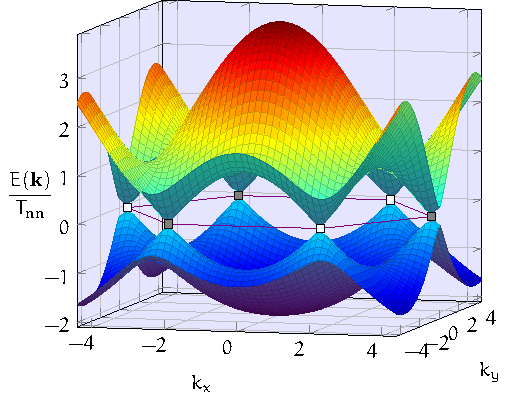
\includegraphics{./img/BandGraph.pdf}
	}\\
	\subcaptionbox[Detalle alrededor de un punto de Dirac]{Detalle alrededor de un punto de Dirac. Se observa la ausencia de una brecha energética entre las bandas, además de la forma de valle o cono de las mismas.\label{fig:diracVicinity}}[0.65\textwidth]{
		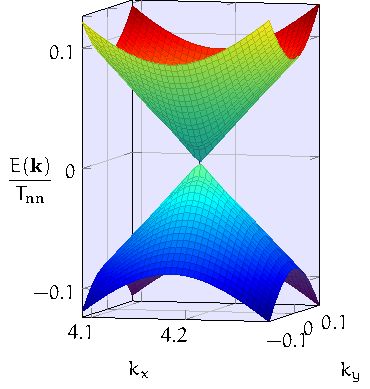
\includegraphics{./img/DiracValley.pdf}
	}
\caption{\label{fig:BandGraphs}Gráficos de la dispersión energética para los electrones $ \pi $ en el grafeno.}
\end{figure}

Debido a que cada átomo de carbono aporta únicamente un electrón $ \pi $ y cada 
electrón puede ocupar exclusivamente un estado de espín arriba o espín abajo, la 
banda baja $ \lambda=- $ se encuentra completamente llena de electrones (banda de 
valencia $ \pi $) y la banda alta $ \lambda=+ $ completamente vacía, o llena de 
huecos (banda de conducción $ \pi* $). De modo que el nivel de Fermi se ubica 
justamente donde las bandas se tocan entre sí.

Es interesante resaltar como las bandas no son simétricas, es decir que no presentan 
una simetría electrón-hueco, la cuál sí se presentaría para el caso en que $ 
T_{\mathtt{nnn}}' = 0 $ en la expresión \eqref{eq:firstapprox}, es decir que las 
correcciones de solapamiento \texttt{nn} y salto \texttt{nnn} son las responsables 
de que se presente este fenómeno.

Los puntos en los que las bandas coinciden se conocen como \emph{Puntos de Dirac} ($ 
D $) y se sitúan donde la dispersión energética \eqref{eq:firstapprox} es igual a 
cero $ E_\lambda(\kvect) = 0 $, lo cual implica que el factor de fase y por ende su 
módulo (y su módulo cuadrado) sean a su vez nulos.
\begin{align*}
	\abs{\alpha\qty(\vector{K^{D}})}^2 = 0 &= 1 + 4\cos(\tfrac{a\sqrt3}{2}k_x^D)\cos(\tfrac{3a}{2}k_y^D) + 4\cos[2](\tfrac{a\sqrt3}{2}k_x^D) \\
	\intertext{Para obtener una solución, escogemos el caso particular $ k_y^D = 0 $}
	\abs{\alpha\qty(\vector{K^{D}})}^2 = 0 &= 1 + 4\cos(\tfrac{a\sqrt3}{2}k_x^D) + 4\cos[2](\tfrac{a\sqrt3}{2}k_x^D) \\
	\abs{\alpha\qty(\vector{K^{D}})}^2 = 0 &= \bqty{1 + 2\cos(\tfrac{a\sqrt3}{2}k_x^D)}^2 \\ 
	\abs{\alpha\qty(\vector{k^{D}})} = 0 &= 1 + 2\cos(\tfrac{a\sqrt3}{2}k_x^D)
\end{align*}
\begin{equation*}
	\therefore -\frac{1}{2} = \cos(\tfrac{a\sqrt3}{2}k_x^D) \\
\end{equation*}
\begin{align*}
	\therefore
	\frac{a\sqrt3}{2}k_x^D &= \pm \frac{2\pi}{3} \\ 
	k_x^D &= \pm \frac{4\pi}{a3\sqrt3}
\end{align*}
\begin{equation}\label{eq:diracPoints}
\therefore \pm\vector{K^{D}} = \pm \frac{4\pi}{a3\sqrt3} \begin{bmatrix} 1 \\ 0 \end{bmatrix}
\end{equation}

De modo que existen dos inequivalentes Puntos de Dirac, $ D $ y $ D' $, que 
corresponden con los puntos cristalográficos $ K $ y $ K' $ \eqref{eq:KK'}. Es 
importante resaltar que estos puntos, aunque situados en el mismo lugar, son 
conceptualmente distintos.

Las bandas $ \pi $ y $ \pi* $ en la vecindad de estos puntos presentan una forma 
aproximable a conos, donde el cambio en la energía respecto a $ \kvect $ es lineal. 
Es debido a esto que se conocen como \emph{Valles de Dirac}. La asociación de esta 
región con Dirac viene dada ya que la aproximación lineal de la relación de 
dispersión alrededor de estos puntos, es similar a la descrita por la ecuación de 
Dirac para fermiones no-masivos (también conocida como la ecuación de Weyl).
	
\section{Propiedades características de los Valles de Dirac}
\subsection{Operador Hamiltoniano efectivo de enlace fuerte}

Partiendo de la matriz Hamiltoniana \eqref{eq:HamiltonianMatrix} se define un operador Hamiltoniano efectivo de enlace fuerte, que para el caso específico del grafeno, tenemos las consideraciones de que es posible fijar $ E_\nu(\kvect) \equiv 0 $ y sustituir entonces la matriz de solapamiento \eqref{eq:TdiagShort} y \eqref{eq:ToffdiagShort}.

\begin{align*}
	\widehat{H}^\mathrm{eff}(\kvect) &= \mathcal{T}(\kvect) \\ 
	\widehat{H}^\mathrm{eff}(\kvect) &= \begin{bmatrix}
	T_{\mathtt{nnn}}\big[\abs{\alpha(\kvect)}^2 - 3\big] & T_{\mathtt{nn}}\alpha^*(\kvect) \\ T_{\mathtt{nn}}\alpha(\kvect) & T_{\mathtt{nnn}}\big[\abs{\alpha(\kvect)}^2 - 3\big]
	\end{bmatrix} \\ 
	\widehat{H}^\mathrm{eff}(\kvect) &= T_{\mathtt{nnn}}\big[\abs{\alpha(\kvect)}^2 - 3\big] \underbrace{\begin{bmatrix}1&0\\0&1\end{bmatrix}}_{\mathbbm{1}} + T_{\mathtt{nn}}\begin{bmatrix} 0 & \alpha^*(\kvect) \\ \alpha(\kvect) & 0 \end{bmatrix}\numberthis\label{eq:TBEffHamiltonian}
\end{align*}

Para obtener los autoestados asociados a nuestro Hamiltoniano efectivo de enlace fuerte, definimos, para facilitar los cálculos, la amplitud de las integrales de salto como nula ($ T_\mathtt{nnn} = 0 $), esto sin perder nuestro resultado esperado ya que al ser proporcional a la matriz unitaria, no afecta significativamente. De forma similar se asume que a las integrales de salto efectivas como nulas ($ T'_\mathtt{nnn} = 0 $).

\begin{subequations}
	\begin{align*}
	\widehat{H}^\mathrm{eff}_{T_\mathtt{nnn}=0}\ket{\psi} (\kvect, \rvect) &= E_{\lambda, T'_\mathtt{nnn}=0} \ket{\psi}(\kvect, \rvect) \\
	\sum_{\nu=0}^{1}\widehat{H}^\mathrm{eff}_{T_\mathtt{nnn}=0}\ket{\Phi_{\nu}}\bra{\Phi_{\nu}}\ket{\psi} (\kvect, \rvect) &= E_{\lambda, T'_\mathtt{nnn}=0} \ket{\psi} (\kvect, \rvect) \\
	\intertext{Multiplicamos la ecuación por un vector compuesto por las funciones de onda \eqref{eq:blochsum} de cada electrón $ \pi $ en la celda unitaria, cuyos subíndices $ \mu =\{0, 1\} $ corresponden a cada subred dentro de la celda unitaria.}
	\sum_{\nu=0}^{1} \begin{bmatrix} \bra{\Phi_{0}}\widehat{H}^\mathrm{eff}_{T_\mathtt{nnn}=0}\ket{\Phi_{\nu}} \bra{\Phi_\nu}\ket{\psi} \\ \bra{\Phi_{1}}\widehat{H}^\mathrm{eff}_{T_\mathtt{nnn}=0}\ket{\Phi_{\nu}} \bra{\Phi_\nu}\ket{\psi} \end{bmatrix}
	(\kvect, \rvect) &= E_{\lambda, T'_\mathtt{nnn}=0}\begin{bmatrix}
	\bra{\Phi_{0}}\ket{\psi}\\\bra{\Phi_{1}}\ket{\psi}
	\end{bmatrix}
	(\kvect, \rvect) \\%\endgroup
	\intertext{Se aplica la sumatoria, sustituyendo los valores correspontiendes a la matrix Hamiltoniana efectiva \eqref{eq:TBEffHamiltonian} y se expande la expresión para la dispersión energética \eqref{eq:firstapprox}.}
	\cancelshade{T_\mathtt{nn}} \begin{bmatrix} \alpha a_1 \\ \alpha^* a_0 \end{bmatrix} (\kvect) &= \lambda \cancelshade{T_{\mathtt{nn}}}\abs{\alpha} \begin{bmatrix} a_0 \\ a_1 \end{bmatrix} (\kvect) \numberthis\label{eq:subRedAmpPre}
	\intertext{Por simplicidad en la notación, se define $ a_0(\kvect) \equiv a(\kvect) $ y $ a_1(\kvect) \equiv b(\kvect) $}
	\begin{bmatrix} 0 & \alpha(\kvect) \\ \alpha^*(\kvect) & 0 \end{bmatrix} \begin{bmatrix} a(\kvect) \\ b(\kvect) \end{bmatrix} &= \lambda \abs{\alpha(\kvect)} \begin{bmatrix} a(\kvect) \\ b(\kvect) \end{bmatrix}\numberthis\label{eq:eigenStatesEQ}
	\end{align*}
\end{subequations}

De modo que los autoestados vienen dados por el espinor
\begin{equation}\label{eq:eigenStates}
\ket{\Psi(\kvect)} = \begin{bmatrix} a(\kvect) \\ b(\kvect) \end{bmatrix}
\end{equation}

Asimismo, de la expresión \eqref{eq:subRedAmpPre} se puede deducir una relación entre las amplitudes de probabilidad de las funciones de ondas de Bloch en las dos sub-redes:

\begin{align*}
	\lambda\abs{\alpha(\kvect)} a(\kvect) &= \alpha(\kvect)b(\kvect) \\
	a_\lambda(\kvect) &= \lambda\frac{\alpha(\kvect)}{\abs{\alpha(\kvect)}} b_\lambda(\kvect) = \lambda\frac{ \cancelshade{\abs{\alpha(\kvect)}} }{ \cancelshade{\abs{\alpha(\kvect)}} } e^{i \operatorname{Arg}\qty(\alpha(\kvect))} b_\lambda(\kvect) \\ 
	a_\lambda(\kvect) &= \lambda e^{i \operatorname{Arg}\qty(\alpha(\kvect))} b_\lambda(\kvect) \numberthis\label{eq:subRedAmp}  
\end{align*}

\subsection{The Continuum Limit}\label{sec:ContinuumLimit}

Para estudiar excitaciones de los estados cuánticos en la proximidad de los puntos de Dirac (equivalente a estudiar excitaciones de bajas energías) es necesario expandir la dispersión energética al rededor de $ \pm\vector{K^{D}} $, de modo que el vector de onda se describe como $ \kvect = \pm\vector{K^{D}} + \qvect $, donde $ \abs{\qvect} \ll \abs{\vector{K^{D}}} \sim \frac{1}{a} $. De modo que el parámetro que gobierna la expansión de la dispersión energética es $ \abs{\qvect} \ll 1 $.

Es notorio que las expresiones de la dispersión energética \eqref{eq:firstapprox} y el Hamiltoniano efectivo \eqref{eq:TBEffHamiltonian}, que elemento necesario a ser expandido es la suma de los factores de fase $ \alpha(\kvect) $, distinguiendo las expansiones al rededor del punto $ D $ del punto $ D' $.

\begin{equation*}
	\alpha(\kvect) = \alpha\pqty{\pm \vector{K^{D}} + \qvect} \equiv \alpha_\pm(\qvect) = 1 + e^{i\pqty{\pm \vector{K^{D}} + \qvect} \cdot \avect1} + e^{i\pqty{\pm \vector{K^{D}} + \qvect} \cdot \avect2} \\
\end{equation*}
Expandiendo $ \vector{K^{D}} $ por \eqref{eq:diracPoints} y los vectores $ \avect1 $ y $ \avect2 $ según \eqref{eq:avectors}
\begin{align*}
	\alpha_\pm(\qvect) &= 1 + e^{\pm i \frac{2\pi\cancelshade{2a\sqrt3}}{3\cancelshade{2a\sqrt3}} \cancelshade{\begin{bsmallmatrix} 1&0 \end{bsmallmatrix} \begin{bsmallmatrix} 1\\\sqrt3 \end{bsmallmatrix}}} e^{i\qvect \cdot \avect1} + e^{\mp i \frac{2\pi\cancelshade{2a\sqrt3}}{3\cancelshade{2a\sqrt3}} \cancelshade{\begin{bsmallmatrix} 1&0 \end{bsmallmatrix} \begin{bsmallmatrix} 1\\-\sqrt3 \end{bsmallmatrix}}} e^{i\qvect \cdot \avect2} \\
	\alpha_\pm(\qvect) &= 1 + e^{\pm i\frac{2\pi}{3}} e^{i\qvect \cdot \avect1} + e^{\mp i\frac{2\pi}{3}} e^{i\qvect \cdot \avect2}\\
	\intertext{Se expanden las exponenciales en series de Taylor y se aproxima truncando las series en polinomios de segundo grado.}
	\alpha_\pm(\qvect) &\approx 1 + e^{\pm i\frac{2\pi}{3}} \bqty{1 + i \qvect \cdot \avect1 - \tfrac{1}{2} \pqty{\qvect \cdot \avect1}^2} + e^{\mp i\frac{2\pi}{3}} \bqty{1 + i \qvect \cdot \avect2 - \tfrac{1}{2} \pqty{\qvect \cdot \avect2}^2}\\\begin{split}
	\alpha_\pm(\qvect) &\approx \bqty{1 + e^{\pm i\frac{2\pi}{3}} + e^{\mp i\frac{2\pi}{3}}} + i \bqty{e^{\pm i\frac{2\pi}{3}} \pqty{\qvect \cdot \avect1} + e^{\mp i\frac{2\pi}{3}}\pqty{\qvect \cdot \avect2}} \\&\phantom\approx- \tfrac{1}{2} \bqty{ e^{\pm i\frac{2\pi}{3}}\pqty{\qvect \cdot \avect1}^2 + e^{\mp i\frac{2\pi}{3}}\pqty{\qvect \cdot \avect2}^2}\end{split}\\
	\alpha_\pm(\qvect) &\approx \alpha_\pm^{(0)}(\qvect) + \alpha_\pm^{(1)}(\qvect) + \alpha_\pm^{(2)}(\qvect) \numberthis\label{eq:expPhaseFactor}
\end{align*}

Analizando la expansión en el orden cero, no es más que la suma de los factores de fase evaluada en los puntos de Dirac, que por definición de los puntos de Dirac, es nulo $ \alpha_\pm^{(0)}(\qvect) = \alpha\qty(\pm \vector{K^{D}}) = 0 $. La expansión se va a limitar hasta el primer orden en $ \abs{\qvect}a $ que es suficiente para describir en su mayor parte las propiedades fundamentales del grafeno. Sin embargo se deja plasmada la posibilidad de extenderse hasta el segundo orden cuya importancia radica en la inclusión de las correcciones dadas por $ T_\mathtt{nnn} $ y contribuciones de segundo orden fuera de la diagonal de la expansión de $ \alpha(\kvect) $.

\subsubsection{Primer orden en $ \abs{\qvect}a $}
	El término de primer orden se desarrolla:
	\begin{align*}
		\alpha_\pm^{(1)}(\qvect) &= i\bqty{e^{\pm i\frac{2\pi}{3}} \pqty{ \frac{a\sqrt3}{2}\begin{bsmallmatrix}q_x&q_y\end{bsmallmatrix} \begin{bsmallmatrix}1\\\sqrt3\end{bsmallmatrix}} + e^{\mp i\frac{2\pi}{3}}\pqty{ \frac{a\sqrt3}{2}\begin{bsmallmatrix}q_x&q_y\end{bsmallmatrix} \begin{bsmallmatrix}-1\\\sqrt3\end{bsmallmatrix}}} \\ 
		&= i \frac{a\sqrt3}{2} \bqty{e^{\pm i\frac{2\pi}{3}} \pqty{q_x + q_y\sqrt3} + e^{\mp i\frac{2\pi}{3}} \pqty{ -q_x + q_y\sqrt3 }} \\ 
		&= i \frac{a\sqrt3}{2} \bqty{ \pqty{ e^{\pm i\frac{2\pi}{3}} - e^{\mp i\frac{2\pi}{3}}} q_x + \sqrt3\pqty{e^{\pm i\frac{2\pi}{3}} + e^{\mp i\frac{2\pi}{3}}} q_y} \\ 
		&= i \frac{a\sqrt3}{2} \bqty{\pqty{ \cancelshade{\cos(\tfrac{2\pi}{3})} \pm i\sin(\tfrac{2\pi}{3}) - \cancelshade{\cos(\tfrac{2\pi}{3})} \pm i\sin(\tfrac{2\pi}{3}) } q_x +  \sqrt3 \pqty{e^{\pm i\frac{2\pi}{3}} + e^{\mp i\frac{2\pi}{3}}} q_y} \\ 
		&= i \frac{a\sqrt3}{2} \bqty{\pm i2\sin(\tfrac{2\pi}{3})q_x + \sqrt3 \pqty{ \cos(\tfrac{2\pi}{3}) \pm \cancelshade{i\sin(\tfrac{2\pi}{3})} + \cos(\tfrac{2\pi}{3}) \mp \cancelshade{i\sin(\tfrac{2\pi}{3})} } q_y} \\ 
		&= i \frac{a\sqrt3}{2} \bqty{\pm i\frac{\cancelshade{2}\sqrt3}{\cancelshade{2}} q_x + 2\sqrt3\cos(\tfrac{2\pi}{3}) q_y } = \frac{3a}{2} \pqty{ \mp q_x - i \frac{\cancelshade{2}}{\cancelshade{2}} q_y } = \mp \frac{3a}{2} \pqty{q_x \pm i q_y} \\ 
		\alpha_\xi^{(1)}(\qvect) &= -\xi \frac{3a}{2} \pqty{q_x +\xi i q_y} \numberthis\label{eq:phaseFactorFirstOrder} 
	\end{align*}

Sustituyendo el resultado anterior en el Hamiltoniano efectivo de enlace fuerte \eqref{eq:TBEffHamiltonian} se obtiene que:

\begin{align*}
	\widehat{H}^{\mathrm{eff}}_\xi (\qvect) &= -\xi T_\mathtt{nn} \frac{3a}{2} \begin{bmatrix} 0 & q_x -\xi i q_y \\ q_x +\xi i q_y & 0 \end{bmatrix} \\
	\widehat{H}^{\mathrm{eff}}_\xi (\qvect) &= \xi \underbrace{\pqty{-\frac{T_\mathtt{nn} 3a}{2\hbar}}}_{v_F} \hbar \pqty{q_x \underbrace{\begin{bsmallmatrix} 0 & 1 \\ 1 & 0 \end{bsmallmatrix}}_{\smash{\sigma^x}} + \xi q_y \underbrace{\begin{bsmallmatrix} 0 & -i \\ i & 0 \end{bsmallmatrix}}_{\smash{\sigma^y}} } \\ 
	\widehat{H}^{\mathrm{eff}}_\xi (\qvect) &= \xi v_F \hbar \pqty{q_x \sigma^x + \xi q_y \sigma^y} \numberthis\label{eq:LowETBEffHamiltonian}
\end{align*}

En las expresiones anteriores se definieron: el \emph{isoespín de valle} $ \xi \equiv \pm $, donde el valor $ \xi = + $ corresponde al punto $ D $ ubicado en $ +\vector{K^D} $ y $ \xi = - $ al punto $ D' $ en $ -\vector{K^D} $, la \emph{velocidad de Fermi} $ v_F \equiv -\frac{T_\mathtt{nn} 3a}{2\hbar} = \frac{\abs{T_\mathtt{nn}} 3a}{2\hbar} $ y las \emph{matrices de Pauli} \[ \sigma^x \equiv \begin{bmatrix} 0 & 1 \\ 1 & 0 \end{bmatrix} \qquad \sigma_y \equiv \begin{bmatrix} 0 & -i \\ i & 0 \end{bmatrix} \]

Como se enunció en párrafos anteriores, el Hamiltoniano de enlace fuerte a bajas energías \eqref{eq:LowETBEffHamiltonian} coincide con la ecuación de Weyl-Dirac.

Sustituyendo \eqref{eq:phaseFactorFirstOrder} en la expresión de la dispersión energética \eqref{eq:firstapprox} con $ \abs{\alpha(\qvect)}^2 = 0 $ se expande:

\begin{align*}
	E_{\lambda, \xi} (\qvect) &= \lambda T_\mathtt{nn} \sqrt{ \alpha(\qvect) \alpha^*(\qvect)} \\ 
	E_{\lambda, \xi} (\qvect) &= \lambda T_\mathtt{nn} \sqrt{\bqty{-\xi \frac{3a}{2} \pqty{q_x +\xi i q_y}} \bqty{-\xi \frac{3a}{2} \pqty{q_x -\xi i q_y}} } \\ 
	E_{\lambda, \xi} (\qvect) &= \lambda T_\mathtt{nn} \frac{3a}{2} \sqrt{ \pqty{q_x +\xi i q_y} \pqty{q_x -\xi i q_y} } \\
	E_{\lambda, \xi} (\qvect) &= \lambda \abs{v_F} \hbar \sqrt{q_x^2 + q_y^2} =  \hbar \abs{\lambda v_F} \sqrt{\abs{\qvect}^2} \\ 
	E_{\lambda, \xi} (\qvect) &= \lambda \hbar \abs{v_F} \abs{\qvect} \numberthis\label{eq:LowEnergyDis}
\end{align*}

De modo que a bajas energías, la dispersión energética es independiente del isoespín 
de valle, que se interpreta como una degeneración doble de los valles; también 
presenta un carácter lineal, que visualmente se puede apreciar mediante un 
acercamiento a la gráfica de la dispersión \eqref{eq:firstapprox} al rededor de un 
punto $ D $ \figref{fig:diracVicinity}.

Finalmente, las amplitudes de probabilidad se expanden mediante la aproximación de 
primer orden
\begin{align*}
	a_{\lambda, \xi} (\qvect) &= \lambda e^{i \operatorname{Arg}\qty(\alpha^{(1)}_{\xi} (\qvect) )} b_{\lambda, \xi} (\qvect) \\ 
	a_{\lambda, \xi} (\qvect) &= \lambda e^{i \operatorname{Arg}\qty( -\xi q_x - i q_y )} b_{\lambda, \xi} (\qvect) \\
	a_{\lambda, \xi} (\qvect) &= - \lambda \xi e^{\xi i \varphi(\qvect)} b_{\lambda, \xi} (\qvect)		
\end{align*}
donde $ \varphi (\qvect) \equiv \angle(\qvect, \hat x) $ es el ángulo polar de $ \qvect $.

De modo que los autoestados, dados por los espinores \eqref{eq:eigenStates}, se 
escriben como
\begin{equation}\label{eq:lowEigenStates}
	\ket{\Psi_{\lambda, \xi} (\qvect)} = \frac{1}{\sqrt2} \begin{bmatrix} - \lambda \xi e^{\xi i \varphi} \\ 1 \end{bmatrix}
\end{equation}
	
% \section{Fenómenos de Transporte}

Para estudiar la dispersión intervalle en el grafeno es necesario revisar los 
principios que rigen los fenómenos de transporte en la escala deseada.

La \emph{ecuación de transporte de \textbf{Boltzmann}} describe el comportamiento estadístico de un sistema termodinámico en un estado fuera del equilibrio. La ecuación surge no por el análisis individual de las posiciones y momentos lineales de cada partícula del sistema, sino considerando una distribución de probabilidad para la posición y el momento lineal de una partícula típica, es decir, la probabilidad de que la partícula ocupe una infinitésima región del espacio de posiciones y momentos lineales en un instante de tiempo.

De esta manera se define entonces la función de densidad de probabilidad $ f(\rvect, \pvect, t) $ la cual cumple que 
\begin{equation}\label{eq:densityDistributionFunction}
\dd{N}  = f(\rvect, \pvect, t) \dd[3]{\rvect} \dd[3]{\pvect}
\end{equation}
donde $ N $ es el número de partículas que tienen posiciones dentro de el volumen $ \dd[3]\rvect $ alrededor de $ \rvect $ y momento lineal dentro del espacio de momento $ \dd[3]\pvect $ alrededor de $ \pvect $, en el instante de tiempo $ t $.

Así que la ecuación de transporte de Boltzmann describe la evolución temporal en el espacio de fase de la función de densidad de probabilidad para una partícula
\begin{equation}\label{eq:BTE}
\pdv{f}{t} + \dv{\rvect}{t} \cdot \grad_{\rvect}{f} + \dv{\pvect}{t} \cdot \nabla_{\pvect}{f} = \left\lgroup \pdv{f}{t} \right\rgroup_{\rlap{colisiones}}
\end{equation} 

El término en el segundo miembro, término dispersivo, corresponde a cambios debido a colisiones, y es la parte más compleja de la ecuación de Boltzmann, si embargo se puede desarrollar mediante teoría perturbacional en la cual aparecen las tasas de transición $ W_i^f $ que describen la probabilidad de que un sistema salte de un estado cuántico inicial $ i $ a un estado final $ f $, ambos accesibles de los sistemas de partículas originales. Esta tasa se define como:
\begin{equation}\label{eq:goldenRule}
W(i, f) = \frac{2\pi}{\hbar} \abs{\bra{i}\widehat{H}'\ket{f}}^2 \delta(E_i - E_f)
\end{equation}
Donde $ \widehat{H}' $ es una pequeña perturbación energética respecto a la energía estable no interactuante $ \widehat{H}_0 $ tal que la energía total del sistema es $ \widehat{H} = \widehat{H}_0 + \widehat{H}' $. Esta expresión para la tasa de transición se conoce como la \emph{regla dorada de \textbf{Fermi}}.

El término dispersivo de la ecuación de Boltzmann equivale a la ganancia neta de partículas en un estado cuántico, que consiste de dos componentes (las siguientes expresiones se trabajan en regímenes de vectores de ondas en lugar de energías o momentos lineales de forma equivalente):
\begin{enumerate}
	\item El incremento de la cantidad de partículas debido a la dispersión desde otros estados cuánticos $ \kvect' $ hacia el estado cuántico en consideración $ \kvect $ \[ + \sum_{\kvect'} f(\rvect, \kvect', t) W(\kvect',\kvect) \]
	\item El decremento de la cantidad de partículas debido a la dispersión desde el estado cuántico en consideración $ \kvect $ hacia otros estados cuánticos $ \kvect' $ \[ - \sum_{\kvect'} f(\rvect, \kvect, t) W(\kvect,\kvect') \]
\end{enumerate}

Si se asume que el sistema se rige por el \emph{principio de balance detallado} que establece que \textquote{En el equilibrio, cada proceso elemental debe ser equilibrado por su proceso inverso}, se tiene entonces que \[ W(i, f) = W(f, i) \]

Así que finalmente el término dispersivo se expresa como:
\begin{equation}\label{eq:BoltzmannColl}
\left\lgroup\pdv{t} f(\rvect, \kvect, t) \right\rgroup_{c} = \sum_{\kvect'} W(\kvect, \kvect') \bqty{ f(\rvect, \kvect', t) - f(\rvect, \kvect, t) }
\end{equation}

Sustituyendo esta expresión para el término dispersivo en la ecuación de Boltzmann, se tiene entonces la igualdad
\begin{equation}\label{eq:BTEexp}
\pdv{f}{t} + \dv{\rvect}{t} \cdot \grad_{\rvect}{f} + \dv{\pvect}{t} \cdot \nabla_{\pvect}{f} = \sum_{\kvect'} W_{\kvect}^{\kvect'} \bqty{ f(\rvect, \kvect', t) - f(\rvect, \kvect, t) }
\end{equation}

Es importante resaltar que la expresión obtenida actúa como base general modificable y escalable para diversas situaciones y condiciones.

\subsection{Aproximación de tiempo de relajación}

La sumatoria discreta sobre los vectores de onda del término dispersivo \eqref{eq:BoltzmannColl} se puede convertir en una integración continua sobre el espacio de fase, y al sustituir esto en la ecuación de Boltzmann \eqref{eq:BTE} se obtendría finalmente una ecuación integro-diferencial en $ f $.

Esta ecuación es muy difícil de resolver en general, por lo cuál la mayoría de las soluciones dependen en una drástica simplificación del término dispersivo mediante la aproximación de tiempo de relajación,
\begin{equation}\label{eq:RTapproximation}
\left\lgroup \pdv{f}{t} \right\rgroup_{c} = - \frac{f - f_0}{\tau} = -\pqty{ f - f_0 } \Gamma
\end{equation}
donde $ \tau $ es el \emph{\textbf{tiempo de relajación}}, $ \Gamma = \tau^{-1} $ es la \emph{tasa de relajación} y $ f_0 $ representa distribución en equilibrio de las partículas, tal como la distribución de Boltzmann, la de Fermi-Dirac, y la de Bose-Einstein.

Esta forma para el término dispersivo asegura que la función de densidad de probabilidad regrese a la distribución en equilibrio si se eliminan todas las fuerzas. Si no hay fuerzas externas ($ \dv{\pvect}{t} = 0 $) y las partículas están distribuidas uniformemente en el espacio ($ \grad_{\rvect}{f} = 0 $), entonces la ecuación de Boltzmann \eqref{eq:BTE} se convierte en:
\begin{align}\label{eq:freeForceBTE}
\pdv{f}{t} + \cancelshade{\dv{\rvect}{t} \cdot \grad_{\rvect}{f}} + \cancelshade{\dv{\pvect}{t} \cdot \nabla_{\pvect}{f}} &= - \frac{f(\kvect, t) - f_0(\kvect)}{\tau(\kvect)} \nonumber\\
\pdv{t} f(\kvect, t)  &= - \frac{f(\kvect, t) - f_0(\kvect)}{\tau(\kvect)}
\end{align}
cuya solución viene dada como
\begin{equation}\label{eq:RTsolution}
f(\kvect, t) = \bqty{f(\kvect, 0) - f_0(\kvect)}e^{-\frac{t}{\tau(\kvect)}} + f_0
\end{equation}
Esta ecuación describe un sistema que comienza en alguna función inicial de densidad de probabilidad fuera del equilibrio $ f(\kvect, 0) $ y vuelve al equilibrio en un tiempo de relajación $ \tau $.
	
	\appendix
\clearpage
\addappheadtotoc
\appendixpage

%\begin{appendices}
	%\chapter{Resolución de la integral de la expresión }
\label{ap:chebMomTraceInt}

La integral resultante de la traza \eqref{eq:chebMomTraceInt} se puede resolver caso por caso para distintas ligaduras sobre los índices $m$ y $n$ antes de escribirla en una expresión general.

\section{Para $ m = n = 0$}
La integral se reduce a 
\begin{equation*}\label{eq:mIsnIsZero}
	\smashoperator{\int_{0}^{2\pi}} \sin[2](x)\cos(mx)\cos(nx)dx = \smashoperator{\int_{0}^{2\pi}} \sin[2](x)dx,
\end{equation*}
en la cuál se aplica la propiedad $\sin[x](x) = \tfrac{1}{2}\bqty{1 - \cos(2x)}$, obteniendo
\begin{align*}
	\smashoperator{\int_{0}^{2\pi}} \sin[2](x)dx &= \tfrac{1}{2} \smashoperator{\int_{0}^{2\pi}} \bqty{1 - \cos(2x)} dx, \\
	\smashoperator{\int_{0}^{2\pi}} \sin[2](x)dx &= \tfrac{1}{2} \bqty{x\big|_{0}^{2\pi} - \tfrac{1}{2}\sin(2x)\big|_{0}^{2\pi}}, \\
	\smashoperator{\int_{0}^{2\pi}} \sin[2](x)dx &= \frac{2\pi}{2} = \pi. \label{eq:intSinsqrd}\numberthis
\end{align*}

\section{Para $ m \neq n = 0$}
Para desarrollar las siguientes integrales es necesario tener en cuenta la relación de ortogonalidad del coseno
\begin{equation}\label{eq:cosineOrthogonality}
	\smashoperator{\int_{0}^{2\pi}} \cos(mx)\cos(nx) dx = \pi \delta^m_n (1 + \delta^m_0).
\end{equation}

Bajo estas ligaduras la integral toma la expresión
\begin{equation*}\label{eq:mIsNotnIsZero}
	\smashoperator{\int_{0}^{2\pi}} \sin[2](x)\cos(mx)\cos(nx)dx = \smashoperator{\int_{0}^{2\pi}} \sin[2](x)\cos(mx)dx.
\end{equation*}
Desarrollando por integración por partes
\begin{align*}
	\smashoperator{\int_{0}^{2\pi}} \sin[2](x)\cos(mx)dx &= \frac{1}{m} \sin(mx)\sin[2](x)\Big|_{0}^{2\pi} - \frac{2}{m}\smashoperator{\int_{0}^{2\pi}} \cos(x)\sin(x)\sin(mx)dx, \\
	\intertext{la integral resultante se puede expandir mediante la propiedad trigonométrica \newline$\sin(\alpha)\sin(\beta) = \frac{1}{2}\bqty{\cos(\alpha - \beta) - \cos(\alpha + \beta)}$}
	\smashoperator{\int_{0}^{2\pi}} \sin[2](x)\cos(mx)dx &= 0 - \frac{1}{m}\smashoperator{\int_{0}^{2\pi}} \cos(x)\bqty{\cos((1 - m)x) - \cos((1 + m)x)}dx, \\
	\smashoperator{\int_{0}^{2\pi}} \sin[2](x)\cos(mx)dx &= -\frac{1}{m}\bqty{\smashoperator{\int_{0}^{2\pi}} \cos(x)\cos((1 - m)x) dx - \smashoperator{\int_{0}^{2\pi}} \cos(x)\cos((1 + m)x)dx}; \\
	\intertext{resolviendo las integrales mediante la relación de ortogonalidad \eqref{eq:cosineOrthogonality}}
	\smashoperator{\int_{0}^{2\pi}} \sin[2](x)\cos(mx)dx &= -\frac{\pi}{m}\bqty{\delta^1_{m-1}(\delta^1_0 + 1) - \delta^{m+1}_1(\delta^1_0 + 1)}. \\
	\intertext{La ligadura $ m \neq 0 \implies \delta^{m+1}_1 = 0 $ y $ \delta^{m-1}_1 = \delta^m_2 $, así que finalmente}
	\smashoperator{\int_{0}^{2\pi}} \sin[2](x)\cos(mx)dx &= -\tfrac{\pi}{2}\delta^m_2. \label{eq:intSinSqrdCosmx}\numberthis
\end{align*}

\section{Para $ m = n \neq 0 $}
Con esto, la integral queda como
\begin{equation*}\label{eq:mIsnIsNotzero}
	\smashoperator{\int_{0}^{2\pi}} \sin[2](x)\cos(mx)\cos(nx)dx = \smashoperator{\int_{0}^{2\pi}} \sin[2](x)\cos[2](mx) dx.
\end{equation*}
Para resolver, se aplica la propiedad trigonométrica $ \cos[2](x) = \frac{1}{2}\bqty{1 + \cos(2x)} $,
\begin{align*}
	\smashoperator{\int_{0}^{2\pi}} \sin[2](x)\cos[2](mx) dx &= \frac{1}{2}\smashoperator{\int_{0}^{2\pi}} \sin[2](x)\bqty{1 + \cos(2mx)} dx, \\ 
	\smashoperator{\int_{0}^{2\pi}} \sin[2](x)\cos[2](mx) dx &= \frac{1}{2}\bqty{\smashoperator{\int_{0}^{2\pi}} \sin[2](x) dx + \smashoperator{\int_{0}^{2\pi}} \sin[2](x)\cos(2mx) dx}, \\
	\intertext{Sustituyendo los valores para la primera y segunda integral por los resultados anteriores \eqref{eq:intSinsqrd} y \eqref{eq:intSinSqrdCosmx} respectivamente,}
	\smashoperator{\int_{0}^{2\pi}} \sin[2](x)\cos[2](mx) dx &= \tfrac{1}{2}\pqty{\pi - \tfrac{\pi}{2}\delta^{2m}_2},\\
	\intertext{lo cual resulta en}
	\smashoperator{\int_{0}^{2\pi}} \sin[2](x)\cos[2](mx) dx &= \tfrac{\pi}{2}\pqty{1 - \tfrac{1}{2}\delta^{m}_1}.\label{eq:intSinSqrdCosmxsqrd}\numberthis
\end{align*}

\section{Para $ m \neq n $}
Finalmente hay que resolver la integral
\begin{equation*}\label{eq:mIsNotn}
	\smashoperator{\int_{0}^{2\pi}} \sin[2](x)\cos(mx)\cos(nx)dx,
\end{equation*}
para ello aplicamos la propiedad trigonométrica $\cos(\alpha)\cos(\beta) = \frac{1}{2}\bqty{\cos(\alpha + \beta) + \cos(\alpha - \beta)}$, obteniendo
\begin{align*}
	\smashoperator{\int_{0}^{2\pi}} \sin[2](x)\cos(mx)\cos(nx)dx &= \frac{1}{2}\smashoperator{\int_{0}^{2\pi}} \sin[2](x)\bqty{\cos((m+n)x) + \cos((m-n)x)}dx, \\ 
	\smashoperator{\int_{0}^{2\pi}} \sin[2](x)\cos(mx)\cos(nx)dx &= \frac{1}{2}\bqty{\smashoperator{\int_{0}^{2\pi}} \sin[2](x)\cos((m+n)x) dx + \smashoperator{\int_{0}^{2\pi}} \sin[2](x) \cos((m-n)x)dx}, \\
	\intertext{sustituyendo lo obtenido de la integral \eqref{eq:intSinSqrdCosmx} tenemos que} 
	\smashoperator{\int_{0}^{2\pi}} \sin[2](x)\cos(mx)\cos(nx)dx &= \tfrac{1}{2}\pqty{-\tfrac{\pi}{2} \delta^2_{m+n} - \tfrac{\pi}{2} \delta^{\abs{m-n}}_2} = -\tfrac{\pi}{4}\pqty{\delta^{m+n}_2 + \delta^{\abs{m-n}}_2}. \label{eq:intSinSqrdCosmxCosnx} \numberthis
\end{align*}
Es sencillo confirmar que estableciendo la condición $ n = 0 $, se recupera lo obtenido en la integral \eqref{eq:intSinSqrdCosmx}.


	
	%\chapter[Conmutador $ \comm{\widehat{U}_0}{\hat{S}_i} $ para la cadena lineal]{Conmutador de los Operadores de Evolución Temporal de la Cadena Lineal y Espín}
\label{ap:commU0S}
	
\begin{align*}
	\comm{\widehat{U}_0}{\hat{S}_i} &= \frac{\hbar}{2}\comm{\exp(\frac{i\widehat{H}_0t}{\hbar})}{\sigma_i}, \\ 
	\comm{\widehat{U}_0}{\hat{S}_i} &= \frac{\hbar}{2}\left[\sum_k\ketbra{k}\exp(\frac{i\epsilon(k)t}{\hbar})\sigma_0\sigma_i - \sigma_i\sum_k\ketbra{k}\exp(\frac{i\epsilon(k)t}{\hbar})\sigma_0\right], \\ 
	\intertext{Recordando que $ \sigma_0 = \mathbbm1_{2\times2} $, entonces}
	\comm{\widehat{U}_0}{\hat{S}_i} &= \frac{\hbar}{2}\sum_k\ketbra{k}\left[\exp(\frac{i\epsilon(k)t}{\hbar})\sigma_i - \exp(\frac{i\epsilon(k)t}{\hbar})\sigma_i\sigma_0\right], \\ 
	\comm{\widehat{U}_0}{\hat{S}_i} &= 0. 
	\numberthis\label{eq:commU0S}
\end{align*}
	
	%\chapter{Operador de Rotación de Espín}
\label{ap:spinRotOP}

\begin{align*}
	\exp(\frac{i\widehat{H}_{\rm ex}t}{\hbar}) &= \exp(\frac{-iJ_{\rm ex}t}{\hbar} \sum_{s} \ketbra{s}{s'} (\hat{u}_{\vector{M}} \cdot \vector{\sigma})_{s, s'}), \\
	\intertext{definiendo $ \Theta(t) \equiv \frac{J_{\rm ex}t}{\hbar} $ y $ \sigma_{u} \equiv \hat{u}_{\vector{M}} \cdot \vector{\sigma} $} 
	\exp(\frac{i\widehat{H}_{\rm ex}t}{\hbar}) &= \exp(-i\Theta \sigma_{u}), \numberthis\label{eq:spinRotOP}\\
	\exp(\frac{i\widehat{H}_{\rm ex}t}{\hbar}) &= \exp(-i\frac{2\Theta}{\hbar} S_{u}),\\
	\exp(\frac{i\widehat{H}_{\rm ex}t}{\hbar}) &= \widehat{R}_u(2\Theta).
\end{align*}

(Tengo entendido que el operador de rotación de espín es $ \widehat{R}(\vector{\hat{n}}, \theta) = \exp(-i\frac{\theta}{\hbar}\vector{S}\cdot\vector{\hat{n}}) = \exp(-i\frac{\theta}{2} \vector{\sigma}\cdot\vector{\hat{n}}) $. Me causa curiosidad que cuando más arriba defines a $ \Theta $ incluyes el signo y no utilizas el factor de 2. Al final no sería muy distinto.)

La expresión \eqref{eq:spinRotOP} se puede reescribir mediante la ecuación de Euler
\begin{align*}
	\exp(-i\Theta \sigma_{u}) &= \cos(\Theta \sigma_{u}) - i\sin(\Theta \sigma_{u}), \\ 
	\intertext{Tomando en cuenta que las matrices de Pauli poseen autovalores $ s_u = \{+1, -1\} $, entonces}
	\exp(-i\Theta \sigma_{u}) &= \sum_{s_u} \ketbra{s_u} \cos(\Theta s_u) - i\sum_{s_u} \ketbra{s_u} \sin(\Theta s_{u}), \\ 
	\exp(-i\Theta \sigma_{u}) &= \sum_{s_u} \ketbra{s_u} \cos(\Theta) - i\sum_{s_u} \ketbra{s_u} s_u \sin(\Theta), \\ 
	\exp(-i\Theta \sigma_{u}) &= \sigma_0\cos(\Theta) - i\sigma_u \sin(\Theta).
\end{align*}
	
	\chapter{Operador de Proyección Cuántico para la Cadena Lineal}
\label{ap:gaussProjOP}

\begin{align*}
	\delta(\widehat{H} - E) &= \lim_{\sigma \to 0} \frac{1}{\sqrt{2\pi\sigma^2}}\exp(-\frac{(\widehat{H} - E)^2}{2\sigma^2}), \\ 
	\delta(\widehat{H} - E) &= \lim_{\sigma \to 0} \frac{1}{\sqrt{2\pi\sigma^2}}\exp(-\frac{(\widehat{H}_0 + \widehat{H}_{\rm ex} - E)^2}{2\sigma^2}), \\ 
	\delta(\widehat{H} - E) &= \lim_{\sigma \to 0} \frac{1}{\sqrt{2\pi\sigma^2}}\exp(-\frac{[(\varepsilon(k) - E)\sigma_0 - J_{\rm ex} \sigma_u ]^2}{2\sigma^2}), \\ 
	\delta(\widehat{H} - E) &= \lim_{\sigma \to 0} \frac{1}{\sqrt{2\pi\sigma^2}}\exp(-\frac{[(\varepsilon(k) - E)^2\sigma_0 - 2J_{\rm ex}(\varepsilon(k) - E) \sigma_u  + J_{\rm ex}^2 \sigma_u^2]}{2\sigma^2}), \\ 
	\intertext{Para las matrices de Pauli se cumple que $ \sigma_u^2 = \sigma_0 $}
	\delta(\widehat{H} - E) &= \lim_{\sigma \to 0} \frac{1}{\sqrt{2\pi\sigma^2}}\exp(-\frac{\left[(\varepsilon(k) - E)^2 + J_{\rm ex}^2 - 2J_{\rm ex}(\varepsilon(k) - E) \sigma_u \right]}{2\sigma^2}), \\ 
	\delta(\widehat{H} - E) &= \lim_{\sigma \to 0} \frac{1}{\sqrt{2\pi\sigma^2}}\exp(-\frac{(\varepsilon(k) - E)^2 + J_{\rm ex}^2}{2\sigma^2}) \exp(\frac{J_{\rm ex}(\varepsilon(k) - E) \sigma_u}{\sigma^2}). \numberthis\label{eq:gaussProjOP}
\end{align*}

Si asumimos el caso particular $ \hat{u}_{\vector M} = \hat{z} \implies \sigma_u = \sigma_z $, el operador de proyección toma la forma
\begin{align*}
	\delta(\widehat{H} - E) &= \lim_{\sigma \to 0} \frac{1}{\sqrt{2\pi\sigma^2}}\exp(-\frac{(\varepsilon(k) - E)^2 + J_{\rm ex}^2}{2\sigma^2}) \exp(\frac{J_{\rm ex}(\varepsilon(k) - E) \sigma_z}{\sigma^2}), \\
	\delta(\widehat{H} - E) &= \sum_s \ketbra{s}{s} \lim_{\sigma \to 0} \frac{1}{\sqrt{2\pi\sigma^2}}\exp(-\frac{(\varepsilon(k) - E)^2 + J_{\rm ex}^2}{2\sigma^2}) \exp(\frac{J_{\rm ex}(\varepsilon(k) - E) s}{\sigma^2}), \\
	\delta(\widehat{H} - E) &= \sum_s \ketbra{s}{s} \lim_{\sigma \to 0} \frac{1}{\sqrt{2\pi\sigma^2}}\exp(-\frac{(\varepsilon(k) - E)^2 - s2J_{\rm ex}(\varepsilon(k) - E) + J_{\rm ex}^2}{2\sigma^2}), \\
	\delta(\widehat{H} - E) &= \sum_s \ketbra{s}{s} \lim_{\sigma \to 0} \frac{1}{\sqrt{2\pi\sigma^2}}\exp(-\frac{(\varepsilon(k) - E - sJ_{\rm ex})^2}{2\sigma^2}), \\
	\delta(\widehat{H} - E) &= \sum_s \ketbra{s}{s} \delta(\varepsilon(k) - E - sJ_{\rm ex}). \numberthis\label{eq:magZProjOP}
\end{align*}

\begin{align*}
	\sum_{k, s} \delta(\varepsilon(k) - sJ_{\rm ex} - E) &= \frac{N}{2\pi} \sum_s \smashoperator{\int_0^{2\pi}} \delta(\varepsilon(ka) - sJ_{\rm ex} - E) d(ka), \\ 
	\sum_{k, s} \delta(\varepsilon(k) - sJ_{\rm ex} - E) &= \frac{N}{2\pi} \sum_s \smashoperator{\int_0^{2\pi}} \delta(-2t\cos(ka) - sJ_{\rm ex} - E) d(ka), \\ 
	\intertext{aplicando la propiedad de la integral de la delta de Dirac compuesta por una función $ f $, $ {\int_R} \delta(f(x)) dx = \sum_i \abs{f'(x_i)}^{-1} $, donde $ x_i $ son los ceros de la función $ f $ en la región $ R $, obtenemos entonces}
	\sum_{k, s} \delta(\varepsilon(k) - sJ_{\rm ex} - E) &= \frac{N}{2\pi} \sum_{s, i}  \abs{2ta\sin(k_ia)}^{-1}, \\ 
	\sum_{k, s} \delta(\varepsilon(k) - sJ_{\rm ex} - E) &= \frac{N}{4\pi\abs{t}a} \sum_{s}  \left[ \abs{\sin(\acos(\frac{E + sJ_{\rm ex}}{-2t}))}^{\rlap{$\scriptstyle -1$}} + \abs{\sin(2\pi - \acos(\frac{E + sJ_{\rm ex}}{-2t}))}^{-1} \right], \\ 
	\sum_{k, s} \delta(\varepsilon(k) - sJ_{\rm ex} - E) &= \frac{N}{2\pi\abs{t}a} \sum_{s} \abs{\sin(\acos(\frac{E + sJ_{\rm ex}}{-2t}))}^{-1}, \\ 
	\sum_{k, s} \delta(\varepsilon(k) - sJ_{\rm ex} - E) &= \frac{N}{2\pi\abs{t}a} \sum_{s} \left[1 - \frac{(E + sJ_{\rm ex})^2
	}{4t^2}\right]^{-1/2}, \\
	\sum_{k, s} \delta(\varepsilon(k) - sJ_{\rm ex} - E) &= \frac{N}{2\pi\abs{t}a} \sum_{s} \frac{2\abs{t}}{\sqrt{4t^2 - (E + sJ_{\rm ex})^2}}, \\
	\sum_{k, s} \delta(\varepsilon(k) - sJ_{\rm ex} - E) &= \frac{N}{\pi a} \left[\frac{1}{\sqrt{4t^2 - (E + J_{\rm ex})^2}} + \frac{1}{\sqrt{4t^2 - (E - J_{\rm ex})^2}} \right]
\end{align*}
	
	%\chapter{Operador de Espín para la Cadena Lineal Magnetizada en z}
\label{ap:S_EV:magZ}

Antes de desarrollar la expresión de la magnetización en $ \hat{\vector z} $ para inyecciones en $ x $ y $ \hat{\vector z} $, es de utilidad definir los elementos de matriz del vector de Pauli en la base de $ \sigma_z $,
\begin{align*}
	\matrixel{s}{ \hat{\vector{S}} }{s'} &= \matrixel{s}{\hat{S}_x}{s'} \hat{\vector x} + \matrixel{s}{\hat{S}_y}{s'} \hat{\vector y} + \matrixel{s}{\hat{S}_z}{s'} \hat{\vector z}, \\
	\matrixel{s}{ \hat{\vector{S}} }{s'} &= (1 - \delta^s_{s'}) \hat{\vector x} + s'i(1- \delta^s_{s'}) \hat{\vector y} + s\delta^s_{s'} \hat{\vector z}, \\ 
	\matrixel{s}{ \hat{\vector{S}} }{s'} &= (1 - \delta^s_{s'}) ( \hat{\vector x} + s'i \hat{\vector y}) + s\delta^s_{s'}\hat{\vector z}.
\end{align*}
Con esta cantidad definida, podemos reescribir cómodamente la expresión de el valor esperado para operador de espín dada una magnetización en $ \hat{\vector z} $ \eqref{eq:S_EV:magZpre}
\begin{equation*}
	\expval{\hat{\vector S}(E_{\rm{F}},t)} = \sum_{k, s} \exp(\frac{i J_{\rm ex }s t}{\hbar}) \bra{ s}\hat{\vector S} \exp(\frac{i\widehat{H}_{\rm ex}t}{\hbar})P(\gamma,\varphi) \delta\left (\varepsilon(k) -J_{\rm ex} \sigma_z  -E\right)P(\gamma,\varphi)\ket{s}.
\end{equation*}
Aplicando la relación de completitud en la base de $ \sigma_z $ y escribiendo la matriz de la delta de Dirac según \eqref{eq:magZProjOP},
\begin{multline}
	\expval{\hat{\vector S}(E_{\rm{F}},t)} = \smashoperator{\sum_{k, s, s'}} \exp(\frac{i J_{\rm ex } t (s - s')}{\hbar}) \matrixel{s}{ \hat{\vector{S}} }{s'} \\
	\bra{s'} P(\gamma, \varphi) \sum_{s''} \ket{s''} \delta\left(\varepsilon(k) - s''J_{\rm ex} -E \right) \bra{s''} P(\gamma, \varphi) \ket{s},\numberthis
\end{multline}
queda entonces una expresión general para las distintas inyecciones electrónicas definidas por $ (\gamma, \varphi) $.

\section{Inyección en $\hat{\vector z}$}
La inyección en $ \hat{\vector z} $ implica que $ P(0, 0) = \ketbra{+} $, por lo cual
\begin{align*}
	\begin{split}
	\expval{\hat{\vector{S}}(E_{\rm{F}},t)} &= \smashoperator{\sum_{k, s, s', s''}} \exp(\frac{i J_{\rm ex } t (s - s')}{\hbar}) \matrixel{s}{ \hat{\vector{S}} }{s'} \\
	&\hspace{13.5em}\braket{s'}{+} \braket{+}{s''} \delta\left(\varepsilon(k) - s''J_{\rm ex} -E \right) \braket{s''}{+} \braket{+}{s}, 
	\end{split}\\
	\begin{split}
	\expval{\hat{\vector{S}}(E_{\rm{F}},t)} &= \smashoperator{\sum_{k, s, s', s''}} \delta^s_+\delta^{s'}_+\delta^{s''}_+ \exp(\frac{i J_{\rm ex } t (s - s')}{\hbar}) \left[(1 - \delta^s_{s'}) ( \hat{\vector x} + s'i \hat{\vector y}) + s\delta^s_{s'}\hat{\vector z}\right] \\
	& \hspace{25em}\delta\left(\varepsilon(k) - s''J_{\rm ex} -E \right),
	\end{split}\\
	\expval{\hat{\vector{S}}(E_{\rm{F}},t)} &= \smashoperator{\sum_{k}} \delta\left(\varepsilon(k) - J_{\rm ex} -E \right) \hat{\vector z}. \numberthis
\end{align*}

\section{Inyección en $\hat{\vector x}$}
La inyección en $ \hat{\vector x} $ implica que $ P(\frac{\pi}{2}, 0) = \ketbra{+, \frac{\pi}{2}, 0} = \ketbra{+, \hat{\vector x}} $, por lo cual
\begin{multline*}
	\expval{\hat{\vector{S}}(E_{\rm{F}},t)} = \smashoperator{\sum_{k, s, s', s''}} \exp(\frac{i J_{\rm ex } t (s - s')}{\hbar}) \matrixel{s}{ \hat{\vector{S}} }{s'} \\ \braket{s'}{+, \hat{\vector x}} \braket{+, \hat{\vector x}}{s''} \delta\left(\varepsilon(k) - s''J_{\rm ex} -E \right) \braket{s''}{+, \hat{\vector x}} \braket{+, \hat{\vector x}}{s},
\end{multline*}
	para los autovectores de las matrices de Pauli, se tiene que $ \braket{s}{+, \hat{\vector x}} = \braket{+, \hat{\vector x}}{s} = \frac{1}{\sqrt2}$ por lo cuál la expresión anterior se reduce a
\begin{align*}
	\expval{\hat{\vector{S}}(E_{\rm{F}},t)} &= \frac{1}{4}\smashoperator{\sum_{k, s, s', s''}} \exp(\frac{i J_{\rm ex } t (s - s')}{\hbar}) \matrixel{s}{ \hat{\vector{S}} }{s'} \delta\left(\varepsilon(k) - s''J_{\rm ex} -E \right), \\
	\expval{\hat{\vector{S}}(E_{\rm{F}},t)} &= \frac{1}{4}\smashoperator{\sum_{k, s, s', s''}} \exp(\frac{i J_{\rm ex } t (s - s')}{\hbar}) \left[(1 - \delta^s_{s'}) ( \hat{\vector x} + s'i \hat{\vector y}) + s\delta^s_{s'}\hat{\vector z} \right] \delta\left(\varepsilon(k) - s''J_{\rm ex} -E \right), \\
	\expval{\hat{\vector{S}}(E_{\rm{F}},t)} &= \frac{1}{4}\smashoperator{\sum_{s}} \left[ \exp(\frac{s2i J_{\rm ex } t}{\hbar}) ( \hat{\vector x} - si \hat{\vector y}) + s\hat{\vector z} \right] \smashoperator{\sum_{k, s''}} \delta\left(\varepsilon(k) - s''J_{\rm ex} -E \right), \\
	\begin{split}
	\expval{\hat{\vector{S}}(E_{\rm{F}},t)} &= \frac{1}{4} \left[ \exp(\frac{2i J_{\rm ex } t}{\hbar}) ( \hat{\vector x} - i \hat{\vector y}) + \exp(\frac{-2i J_{\rm ex } t}{\hbar}) ( \hat{\vector x} + i \hat{\vector y}) + \hat{\vector z} - \hat{\vector z} \right] \\
	&\hspace{21.5em} \smashoperator{\sum_{k, s''}} \delta\left(\varepsilon(k) - s''J_{\rm ex} -E \right), 
	\end{split}\\
	\expval{\hat{\vector{S}}(E_{\rm{F}},t)} &= \frac{1}{2} \left[ \Re{\exp(\frac{2i J_{\rm ex } t}{\hbar})} \hat{\vector x} + \Im{\exp(\frac{2i J_{\rm ex } t}{\hbar})} \hat{\vector y} \right]  \smashoperator{\sum_{k, s}} \delta\left(\varepsilon(k) - sJ_{\rm ex} -E \right), \\
	\expval{\hat{\vector{S}}(E_{\rm{F}},t)} &= \frac{1}{2} \left[ \cos(\frac{2 J_{\rm ex } t}{\hbar}) \hat{\vector x} + \sin(\frac{2 J_{\rm ex } t}{\hbar}) \hat{\vector y} \right]  \smashoperator{\sum_{k, s}} \delta\left(\varepsilon(k) - sJ_{\rm ex} -E \right). \numberthis
\end{align*}
%\end{appendices}
	
	\backmatter
	
	\fancyhead[LE,RO]{}
%\nocite{*}
\addcontentsline{toc}{chapter}{Bibliografía}
\printbibliography
	
	\end{document}
